\documentclass[twoside]{book}

% Packages required by doxygen
\usepackage{fixltx2e}
\usepackage{calc}
\usepackage{doxygen}
\usepackage[export]{adjustbox} % also loads graphicx
\usepackage{graphicx}
\usepackage[utf8]{inputenc}
\usepackage{makeidx}
\usepackage{multicol}
\usepackage{multirow}
\PassOptionsToPackage{warn}{textcomp}
\usepackage{textcomp}
\usepackage[nointegrals]{wasysym}
\usepackage[table]{xcolor}

% NLS support packages
\usepackage[T2A]{fontenc}
\usepackage[russian]{babel}

% Font selection
\usepackage[T1]{fontenc}
\usepackage[scaled=.90]{helvet}
\usepackage{courier}
\usepackage{amssymb}
\usepackage{sectsty}
\renewcommand{\familydefault}{\sfdefault}
\allsectionsfont{%
  \fontseries{bc}\selectfont%
  \color{darkgray}%
}
\renewcommand{\DoxyLabelFont}{%
  \fontseries{bc}\selectfont%
  \color{darkgray}%
}
\newcommand{\+}{\discretionary{\mbox{\scriptsize$\hookleftarrow$}}{}{}}

% Page & text layout
\usepackage{geometry}
\geometry{%
  a4paper,%
  top=2.5cm,%
  bottom=2.5cm,%
  left=2.5cm,%
  right=2.5cm%
}
\tolerance=750
\hfuzz=15pt
\hbadness=750
\setlength{\emergencystretch}{15pt}
\setlength{\parindent}{0cm}
\setlength{\parskip}{3ex plus 2ex minus 2ex}
\makeatletter
\renewcommand{\paragraph}{%
  \@startsection{paragraph}{4}{0ex}{-1.0ex}{1.0ex}{%
    \normalfont\normalsize\bfseries\SS@parafont%
  }%
}
\renewcommand{\subparagraph}{%
  \@startsection{subparagraph}{5}{0ex}{-1.0ex}{1.0ex}{%
    \normalfont\normalsize\bfseries\SS@subparafont%
  }%
}
\makeatother

% Headers & footers
\usepackage{fancyhdr}
\pagestyle{fancyplain}
\fancyhead[LE]{\fancyplain{}{\bfseries\thepage}}
\fancyhead[CE]{\fancyplain{}{}}
\fancyhead[RE]{\fancyplain{}{\bfseries\leftmark}}
\fancyhead[LO]{\fancyplain{}{\bfseries\rightmark}}
\fancyhead[CO]{\fancyplain{}{}}
\fancyhead[RO]{\fancyplain{}{\bfseries\thepage}}
\fancyfoot[LE]{\fancyplain{}{}}
\fancyfoot[CE]{\fancyplain{}{}}
\fancyfoot[RE]{\fancyplain{}{\bfseries\scriptsize Создано системой Doxygen }}
\fancyfoot[LO]{\fancyplain{}{\bfseries\scriptsize Создано системой Doxygen }}
\fancyfoot[CO]{\fancyplain{}{}}
\fancyfoot[RO]{\fancyplain{}{}}
\renewcommand{\footrulewidth}{0.4pt}
\renewcommand{\chaptermark}[1]{%
  \markboth{#1}{}%
}
\renewcommand{\sectionmark}[1]{%
  \markright{\thesection\ #1}%
}

% Indices & bibliography
\usepackage{natbib}
\usepackage[titles]{tocloft}
\setcounter{tocdepth}{3}
\setcounter{secnumdepth}{5}
\makeindex

% Hyperlinks (required, but should be loaded last)
\usepackage{ifpdf}
\ifpdf
  \usepackage[pdftex,pagebackref=true]{hyperref}
\else
  \usepackage[ps2pdf,pagebackref=true]{hyperref}
\fi
\hypersetup{%
  colorlinks=true,%
  linkcolor=blue,%
  citecolor=blue,%
  unicode%
}

% Custom commands
\newcommand{\clearemptydoublepage}{%
  \newpage{\pagestyle{empty}\cleardoublepage}%
}

\usepackage{caption}
\captionsetup{labelsep=space,justification=centering,font={bf},singlelinecheck=off,skip=4pt,position=top}

%===== C O N T E N T S =====

\begin{document}

% Titlepage & ToC
\hypersetup{pageanchor=false,
             bookmarksnumbered=true,
             pdfencoding=unicode
            }
\pagenumbering{alph}
\begin{titlepage}
\vspace*{7cm}
\begin{center}%
{\Large Race game }\\
\vspace*{1cm}
{\large Создано системой Doxygen 1.8.13}\\
\end{center}
\end{titlepage}
\clearemptydoublepage
\pagenumbering{roman}
\tableofcontents
\clearemptydoublepage
\pagenumbering{arabic}
\hypersetup{pageanchor=true}

%--- Begin generated contents ---
\chapter{Игра \char`\"{}Забег\char`\"{}}
\label{index}\hypertarget{index}{}Программа -\/ это реализация игры \char`\"{}Забег\char`\"{}.

\subsection*{Информация}

Проект написан на языке C с использование библиотеки allegro. Unit-\/тесты были написаны с истользованием фреймворка Unity.

\subsubsection*{Скриншот}



\subsubsection*{Правила игры}

Ваша задача -\/ как можно быстрее пересечь финишную черту.

\subsubsection*{Управление}

Для старта игры небходимо нажать клавишу \char`\"{}\+Enter\char`\"{}.

После старта игры для увеличения скорости игрока нужно нажимать клавиши \char`\"{}стрелка влево\char`\"{} и \char`\"{}стрелка вправо\char`\"{}, чем чаще нажимать, тем выше скорость.

После финиширования для выхода из игры небоходимо нажать кливишу \char`\"{}\+Enter\char`\"{}.

\subsubsection*{Структура директории}

Файлы в директории лежат следующим образом\+:

\tabulinesep=1mm
\begin{longtabu} spread 0pt [c]{*{2}{|X[-1]}|}
\hline
\rowcolor{\tableheadbgcolor}\textbf{ Каталог }&\textbf{ Описание  }\\\cline{1-2}
\endfirsthead
\hline
\endfoot
\hline
\rowcolor{\tableheadbgcolor}\textbf{ Каталог }&\textbf{ Описание  }\\\cline{1-2}
\endhead
src/ &файлы исходного кода \\\cline{1-2}
src/res &ресурсы игры \\\cline{1-2}
src/test &unit-\/тесты \\\cline{1-2}
doc/ &документация \\\cline{1-2}
doc/res/ &ресурсы для документации \\\cline{1-2}
\end{longtabu}
\subsubsection*{Сборка}

Для того, чтобы собрать проект напишите следующее\+: 
\begin{DoxyCode}
make
\end{DoxyCode}
 Чтобы восстановить все с нуля, выполните следующее действие\+: 
\begin{DoxyCode}
make clean
\end{DoxyCode}
 Для запуска тестов необходимо ввести следующую команду\+: 
\begin{DoxyCode}
make D\_UNITY=../Unity check
\end{DoxyCode}
 Для сборки документации\+: 
\begin{DoxyCode}
make doxygen
\end{DoxyCode}
 Для сборки документации в формате P\+DF\+: 
\begin{DoxyCode}
make pdf
\end{DoxyCode}
 Для сборки документации в формате H\+T\+ML\+: 
\begin{DoxyCode}
make html
\end{DoxyCode}


\subsection*{Авторы}


\begin{DoxyItemize}
\item {\bfseries Пупкин Васий} -\/ \href{mailto:pupkin@mail.ru}{\tt pupkin@mail.\+ru}
\end{DoxyItemize}

\subsection*{Лицензия}

This project is licensed under the M\+IT License -\/ see the \mbox{[}L\+I\+C\+E\+N\+SE\mbox{]}(L\+I\+C\+E\+N\+SE) file for details 
\chapter{Алфавитный указатель структур данных}
\section{Структуры данных}
Структуры данных с их кратким описанием.\begin{DoxyCompactList}
\item\contentsline{section}{\hyperlink{structfield__view}{field\+\_\+view} \\*Структура, которая описывает отображение игрового поля }{\pageref{structfield__view}}{}
\item\contentsline{section}{\hyperlink{structgame__model}{game\+\_\+model} \\*Структура, которая описывает модель игры }{\pageref{structgame__model}}{}
\item\contentsline{section}{\hyperlink{structgame__view}{game\+\_\+view} \\*Структура, которая описывает отображение игры }{\pageref{structgame__view}}{}
\item\contentsline{section}{\hyperlink{structlabel__view}{label\+\_\+view} \\*Структура, которая описывает элемент интерфейса\+: \char`\"{}надпись\char`\"{} }{\pageref{structlabel__view}}{}
\item\contentsline{section}{\hyperlink{structplayer__model}{player\+\_\+model} \\*Структура, которая описывает модель игрока }{\pageref{structplayer__model}}{}
\item\contentsline{section}{\hyperlink{structplayer__view}{player\+\_\+view} \\*Структура, которая описывает отображение игрока }{\pageref{structplayer__view}}{}
\item\contentsline{section}{\hyperlink{structtimer__model}{timer\+\_\+model} \\*Структура, которая описывает модель таймеров }{\pageref{structtimer__model}}{}
\item\contentsline{section}{\hyperlink{structtimer__view}{timer\+\_\+view} \\*Структура, которая описывает отображение таймеров }{\pageref{structtimer__view}}{}
\end{DoxyCompactList}

\chapter{Список файлов}
\section{Файлы}
Полный список файлов.\begin{DoxyCompactList}
\item\contentsline{section}{src/\hyperlink{error__report_8c}{error\+\_\+report.\+c} \\*Файл, в котором реализованы функции логирования ошибок }{\pageref{error__report_8c}}{}
\item\contentsline{section}{src/\hyperlink{error__report_8h}{error\+\_\+report.\+h} \\*Файл, в котором опеределены функции логирования ошибок }{\pageref{error__report_8h}}{}
\item\contentsline{section}{src/\hyperlink{field__view_8c}{field\+\_\+view.\+c} \\*Файл, в котором реализованы функции для работы с отображением игрового поля }{\pageref{field__view_8c}}{}
\item\contentsline{section}{src/\hyperlink{field__view_8h}{field\+\_\+view.\+h} \\*Файл, в котором опеределены функции для работы с отображением игрового поля }{\pageref{field__view_8h}}{}
\item\contentsline{section}{src/\hyperlink{game__model_8c}{game\+\_\+model.\+c} }{\pageref{game__model_8c}}{}
\item\contentsline{section}{src/\hyperlink{game__model_8h}{game\+\_\+model.\+h} \\*Файл, в котором опеределены функции для работы с моделью игры }{\pageref{game__model_8h}}{}
\item\contentsline{section}{src/\hyperlink{game__view_8c}{game\+\_\+view.\+c} \\*Файл, в котором опеределены функции для работы с отображением игры }{\pageref{game__view_8c}}{}
\item\contentsline{section}{src/\hyperlink{game__view_8h}{game\+\_\+view.\+h} \\*Файл, в котором опеределены функции для работы с отображением игры }{\pageref{game__view_8h}}{}
\item\contentsline{section}{src/\hyperlink{label__view_8c}{label\+\_\+view.\+c} \\*Файл, в котором реализованы функции для работы с элементом интерфейса\+: \char`\"{}надпись\char`\"{} }{\pageref{label__view_8c}}{}
\item\contentsline{section}{src/\hyperlink{label__view_8h}{label\+\_\+view.\+h} \\*Файл, в котором опеределены функции для работы с элементом интерфейса\+: \char`\"{}надпись\char`\"{} }{\pageref{label__view_8h}}{}
\item\contentsline{section}{src/\hyperlink{main_8c}{main.\+c} \\*Файл, в котором создается и запускается игра }{\pageref{main_8c}}{}
\item\contentsline{section}{src/\hyperlink{player__model_8c}{player\+\_\+model.\+c} \\*Файл, в котором реализованы функции для работы с моделью игрока }{\pageref{player__model_8c}}{}
\item\contentsline{section}{src/\hyperlink{player__model_8h}{player\+\_\+model.\+h} \\*Файл, в котором опеределены функции для работы с моделью игрока }{\pageref{player__model_8h}}{}
\item\contentsline{section}{src/\hyperlink{player__view_8c}{player\+\_\+view.\+c} }{\pageref{player__view_8c}}{}
\item\contentsline{section}{src/\hyperlink{player__view_8h}{player\+\_\+view.\+h} \\*Файл, в котором опеределены функции для работы с отображением игрока }{\pageref{player__view_8h}}{}
\item\contentsline{section}{src/\hyperlink{rectangle__view_8c}{rectangle\+\_\+view.\+c} \\*Файл, в котором реализованы функции для работы с элементом интерфейса\+: \char`\"{}прямоугольник\char`\"{} }{\pageref{rectangle__view_8c}}{}
\item\contentsline{section}{src/\hyperlink{rectangle__view_8h}{rectangle\+\_\+view.\+h} \\*Файл, в котором опеределены функции для работы с элементом интерфейса\+: \char`\"{}прямоугольник\char`\"{} }{\pageref{rectangle__view_8h}}{}
\item\contentsline{section}{src/\hyperlink{timer__model_8c}{timer\+\_\+model.\+c} }{\pageref{timer__model_8c}}{}
\item\contentsline{section}{src/\hyperlink{timer__model_8h}{timer\+\_\+model.\+h} \\*Файл, в котором опеределены функции для работы с моделью таймеров }{\pageref{timer__model_8h}}{}
\item\contentsline{section}{src/\hyperlink{timer__view_8c}{timer\+\_\+view.\+c} \\*Файл, в котором реализованы функции для работы с отображением таймеров }{\pageref{timer__view_8c}}{}
\item\contentsline{section}{src/\hyperlink{timer__view_8h}{timer\+\_\+view.\+h} \\*Файл, в котором опеределены функции для работы с отображением таймеров }{\pageref{timer__view_8h}}{}
\item\contentsline{section}{src/test/\hyperlink{runner_8c}{runner.\+c} \\*Функция запуска всех тестов }{\pageref{runner_8c}}{}
\item\contentsline{section}{src/test/\hyperlink{test___game_model_8c}{test\+\_\+\+Game\+Model.\+c} \\*Файл тестирующий игровую модель }{\pageref{test___game_model_8c}}{}
\item\contentsline{section}{src/test/\hyperlink{test___player_model_8c}{test\+\_\+\+Player\+Model.\+c} \\*Файл тестирующий модель игрока }{\pageref{test___player_model_8c}}{}
\item\contentsline{section}{src/test/\hyperlink{test___timer_model_8c}{test\+\_\+\+Timer\+Model.\+c} \\*Файл тестирующий модель таймеров }{\pageref{test___timer_model_8c}}{}
\end{DoxyCompactList}

\chapter{Структуры данных}
\hypertarget{structfield__view}{}\section{Структура field\+\_\+view}
\label{structfield__view}\index{field\+\_\+view@{field\+\_\+view}}


Структура, которая описывает отображение игрового поля.  




{\ttfamily \#include $<$field\+\_\+view.\+h$>$}



Граф связей класса field\+\_\+view\+:\nopagebreak
\begin{figure}[H]
\begin{center}
\leavevmode
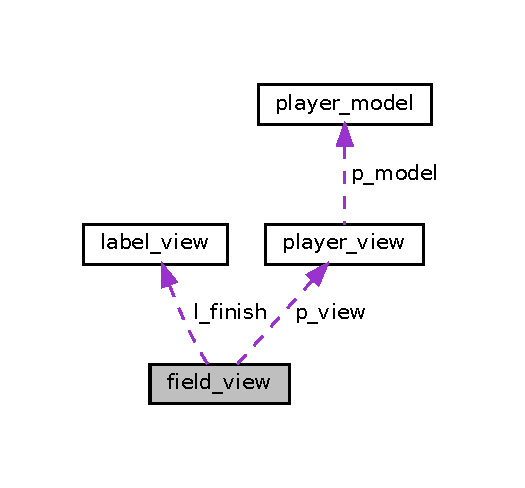
\includegraphics[width=252pt]{structfield__view__coll__graph}
\end{center}
\end{figure}
\subsection*{Поля данных}
\begin{DoxyCompactItemize}
\item 
A\+L\+L\+E\+G\+R\+O\+\_\+\+B\+I\+T\+M\+AP $\ast$ \hyperlink{structfield__view_ab53c9a1f28f08baf51ad715a0959d7bd}{r\+\_\+backgroud}
\begin{DoxyCompactList}\small\item\em Адрес прямоугольника фона. \end{DoxyCompactList}\item 
A\+L\+L\+E\+G\+R\+O\+\_\+\+B\+I\+T\+M\+AP $\ast$ \hyperlink{structfield__view_a55858cc4e1caeeea539ff16ddd1baa79}{r\+\_\+border}
\begin{DoxyCompactList}\small\item\em Адрес прямоугольника рамки. \end{DoxyCompactList}\item 
\hyperlink{structplayer__view}{player\+\_\+view} $\ast$ \hyperlink{structfield__view_ab3016ab1d95a4391f499cb754981d783}{p\+\_\+view}
\begin{DoxyCompactList}\small\item\em Адрес отображения игрока. \end{DoxyCompactList}\item 
\hyperlink{structlabel__view}{label\+\_\+view} $\ast$ \hyperlink{structfield__view_ab27a2b7d362ab502ba9430d59236f5ef}{l\+\_\+finish}
\begin{DoxyCompactList}\small\item\em Адрес надпси \char`\"{}\+Finish\char`\"{}. \end{DoxyCompactList}\end{DoxyCompactItemize}


\subsection{Подробное описание}
Структура, которая описывает отображение игрового поля. 

\subsection{Поля}
\mbox{\Hypertarget{structfield__view_ab27a2b7d362ab502ba9430d59236f5ef}\label{structfield__view_ab27a2b7d362ab502ba9430d59236f5ef}} 
\index{field\+\_\+view@{field\+\_\+view}!l\+\_\+finish@{l\+\_\+finish}}
\index{l\+\_\+finish@{l\+\_\+finish}!field\+\_\+view@{field\+\_\+view}}
\subsubsection{\texorpdfstring{l\+\_\+finish}{l\_finish}}
{\footnotesize\ttfamily \hyperlink{structlabel__view}{label\+\_\+view}$\ast$ field\+\_\+view\+::l\+\_\+finish}



Адрес надпси \char`\"{}\+Finish\char`\"{}. 

\mbox{\Hypertarget{structfield__view_ab3016ab1d95a4391f499cb754981d783}\label{structfield__view_ab3016ab1d95a4391f499cb754981d783}} 
\index{field\+\_\+view@{field\+\_\+view}!p\+\_\+view@{p\+\_\+view}}
\index{p\+\_\+view@{p\+\_\+view}!field\+\_\+view@{field\+\_\+view}}
\subsubsection{\texorpdfstring{p\+\_\+view}{p\_view}}
{\footnotesize\ttfamily \hyperlink{structplayer__view}{player\+\_\+view}$\ast$ field\+\_\+view\+::p\+\_\+view}



Адрес отображения игрока. 

\mbox{\Hypertarget{structfield__view_ab53c9a1f28f08baf51ad715a0959d7bd}\label{structfield__view_ab53c9a1f28f08baf51ad715a0959d7bd}} 
\index{field\+\_\+view@{field\+\_\+view}!r\+\_\+backgroud@{r\+\_\+backgroud}}
\index{r\+\_\+backgroud@{r\+\_\+backgroud}!field\+\_\+view@{field\+\_\+view}}
\subsubsection{\texorpdfstring{r\+\_\+backgroud}{r\_backgroud}}
{\footnotesize\ttfamily A\+L\+L\+E\+G\+R\+O\+\_\+\+B\+I\+T\+M\+AP$\ast$ field\+\_\+view\+::r\+\_\+backgroud}



Адрес прямоугольника фона. 

\mbox{\Hypertarget{structfield__view_a55858cc4e1caeeea539ff16ddd1baa79}\label{structfield__view_a55858cc4e1caeeea539ff16ddd1baa79}} 
\index{field\+\_\+view@{field\+\_\+view}!r\+\_\+border@{r\+\_\+border}}
\index{r\+\_\+border@{r\+\_\+border}!field\+\_\+view@{field\+\_\+view}}
\subsubsection{\texorpdfstring{r\+\_\+border}{r\_border}}
{\footnotesize\ttfamily A\+L\+L\+E\+G\+R\+O\+\_\+\+B\+I\+T\+M\+AP$\ast$ field\+\_\+view\+::r\+\_\+border}



Адрес прямоугольника рамки. 



Объявления и описания членов структуры находятся в файле\+:\begin{DoxyCompactItemize}
\item 
src/\hyperlink{field__view_8h}{field\+\_\+view.\+h}\end{DoxyCompactItemize}

\hypertarget{structgame__model}{}\section{Структура game\+\_\+model}
\label{structgame__model}\index{game\+\_\+model@{game\+\_\+model}}


Структура, которая описывает модель игры.  




{\ttfamily \#include $<$game\+\_\+model.\+h$>$}



Граф связей класса game\+\_\+model\+:\nopagebreak
\begin{figure}[H]
\begin{center}
\leavevmode
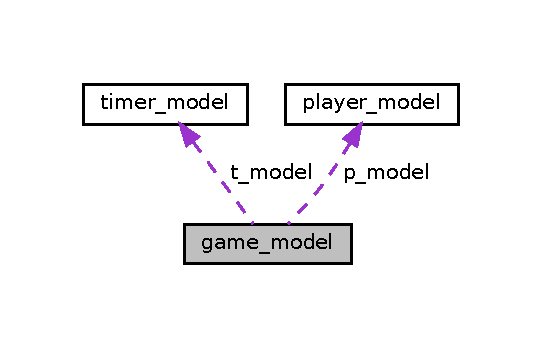
\includegraphics[width=260pt]{structgame__model__coll__graph}
\end{center}
\end{figure}
\subsection*{Поля данных}
\begin{DoxyCompactItemize}
\item 
\hyperlink{structplayer__model}{player\+\_\+model} $\ast$ \hyperlink{structgame__model_a3bcbf217f1b8c8f3e2407b852da268ed}{p\+\_\+model}
\begin{DoxyCompactList}\small\item\em Адрес модели игрока. \end{DoxyCompactList}\item 
\hyperlink{structtimer__model}{timer\+\_\+model} $\ast$ \hyperlink{structgame__model_aadcf1b0427739bb95070a015c4b43988}{t\+\_\+model}
\begin{DoxyCompactList}\small\item\em Адрес модели таймеров. \end{DoxyCompactList}\item 
unsigned int $\ast$ \hyperlink{structgame__model_abf2236d6bb182f60659d811a096ba0b3}{num\+\_\+push}
\begin{DoxyCompactList}\small\item\em Количество нажатий клавиш влево и вправо, в каждую секунду игры. \end{DoxyCompactList}\item 
\hyperlink{game__model_8h_ab56b05c2bb34d1168dc2576c83a1e287}{key\+\_\+type} \hyperlink{structgame__model_a33e6b79824419341cc8aa5246f0836d4}{last\+\_\+key}
\begin{DoxyCompactList}\small\item\em Тип клавиши нажатой в последний раз. \end{DoxyCompactList}\end{DoxyCompactItemize}


\subsection{Подробное описание}
Структура, которая описывает модель игры. 

\subsection{Поля}
\mbox{\Hypertarget{structgame__model_a33e6b79824419341cc8aa5246f0836d4}\label{structgame__model_a33e6b79824419341cc8aa5246f0836d4}} 
\index{game\+\_\+model@{game\+\_\+model}!last\+\_\+key@{last\+\_\+key}}
\index{last\+\_\+key@{last\+\_\+key}!game\+\_\+model@{game\+\_\+model}}
\subsubsection{\texorpdfstring{last\+\_\+key}{last\_key}}
{\footnotesize\ttfamily \hyperlink{game__model_8h_ab56b05c2bb34d1168dc2576c83a1e287}{key\+\_\+type} game\+\_\+model\+::last\+\_\+key}



Тип клавиши нажатой в последний раз. 

\mbox{\Hypertarget{structgame__model_abf2236d6bb182f60659d811a096ba0b3}\label{structgame__model_abf2236d6bb182f60659d811a096ba0b3}} 
\index{game\+\_\+model@{game\+\_\+model}!num\+\_\+push@{num\+\_\+push}}
\index{num\+\_\+push@{num\+\_\+push}!game\+\_\+model@{game\+\_\+model}}
\subsubsection{\texorpdfstring{num\+\_\+push}{num\_push}}
{\footnotesize\ttfamily unsigned int$\ast$ game\+\_\+model\+::num\+\_\+push}



Количество нажатий клавиш влево и вправо, в каждую секунду игры. 

\mbox{\Hypertarget{structgame__model_a3bcbf217f1b8c8f3e2407b852da268ed}\label{structgame__model_a3bcbf217f1b8c8f3e2407b852da268ed}} 
\index{game\+\_\+model@{game\+\_\+model}!p\+\_\+model@{p\+\_\+model}}
\index{p\+\_\+model@{p\+\_\+model}!game\+\_\+model@{game\+\_\+model}}
\subsubsection{\texorpdfstring{p\+\_\+model}{p\_model}}
{\footnotesize\ttfamily \hyperlink{structplayer__model}{player\+\_\+model}$\ast$ game\+\_\+model\+::p\+\_\+model}



Адрес модели игрока. 

\mbox{\Hypertarget{structgame__model_aadcf1b0427739bb95070a015c4b43988}\label{structgame__model_aadcf1b0427739bb95070a015c4b43988}} 
\index{game\+\_\+model@{game\+\_\+model}!t\+\_\+model@{t\+\_\+model}}
\index{t\+\_\+model@{t\+\_\+model}!game\+\_\+model@{game\+\_\+model}}
\subsubsection{\texorpdfstring{t\+\_\+model}{t\_model}}
{\footnotesize\ttfamily \hyperlink{structtimer__model}{timer\+\_\+model}$\ast$ game\+\_\+model\+::t\+\_\+model}



Адрес модели таймеров. 



Объявления и описания членов структуры находятся в файле\+:\begin{DoxyCompactItemize}
\item 
src/\hyperlink{game__model_8h}{game\+\_\+model.\+h}\end{DoxyCompactItemize}

\hypertarget{structgame__view}{}\section{Структура game\+\_\+view}
\label{structgame__view}\index{game\+\_\+view@{game\+\_\+view}}


Структура, которая описывает отображение игры.  




{\ttfamily \#include $<$game\+\_\+view.\+h$>$}



Граф связей класса game\+\_\+view\+:\nopagebreak
\begin{figure}[H]
\begin{center}
\leavevmode
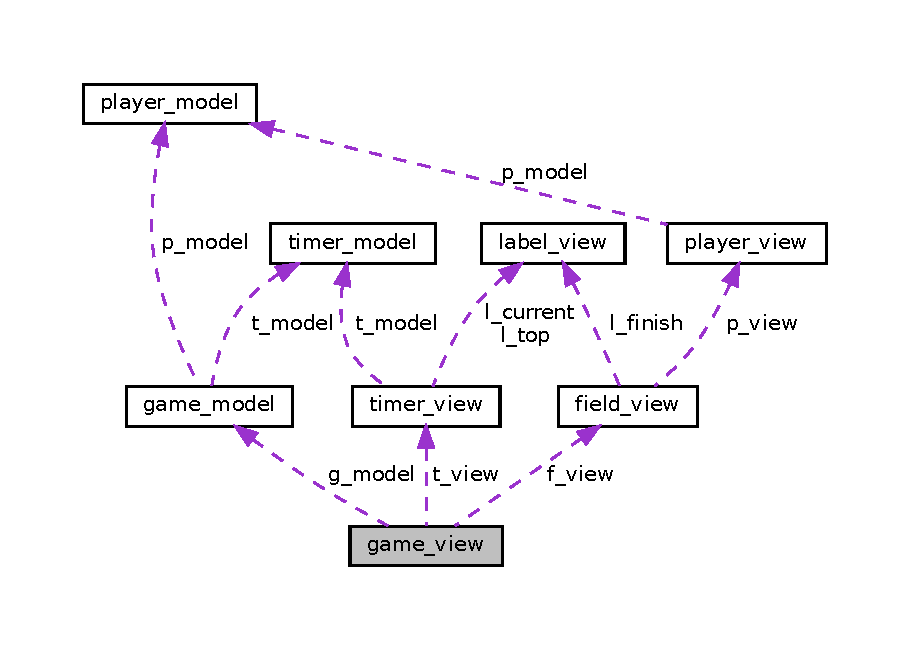
\includegraphics[width=350pt]{structgame__view__coll__graph}
\end{center}
\end{figure}
\subsection*{Поля данных}
\begin{DoxyCompactItemize}
\item 
\hyperlink{structgame__model}{game\+\_\+model} $\ast$ \hyperlink{structgame__view_a09b15cc54d9bc6ea5e6d67bd27639b47}{g\+\_\+model}
\begin{DoxyCompactList}\small\item\em Модель игры. \end{DoxyCompactList}\item 
\hyperlink{structtimer__view}{timer\+\_\+view} $\ast$ \hyperlink{structgame__view_a0490cc44940b39d3be15cb3d543988f2}{t\+\_\+view}
\begin{DoxyCompactList}\small\item\em Отображение таймеров. \end{DoxyCompactList}\item 
\hyperlink{structfield__view}{field\+\_\+view} $\ast$ \hyperlink{structgame__view_a1a070c6c14bf9c04398b2aab5609ec81}{f\+\_\+view}
\begin{DoxyCompactList}\small\item\em Отображение поля игры. \end{DoxyCompactList}\item 
A\+L\+L\+E\+G\+R\+O\+\_\+\+D\+I\+S\+P\+L\+AY $\ast$ \hyperlink{structgame__view_ae9721ac01fbc40ea44587bca447a71d3}{display}
\begin{DoxyCompactList}\small\item\em Адрес дисплея. \end{DoxyCompactList}\item 
A\+L\+L\+E\+G\+R\+O\+\_\+\+E\+V\+E\+N\+T\+\_\+\+Q\+U\+E\+UE $\ast$ \hyperlink{structgame__view_a2329d90e0f5234304cc7039e94e9ce33}{event\+\_\+queue}
\begin{DoxyCompactList}\small\item\em Адрес очереди событий. \end{DoxyCompactList}\item 
A\+L\+L\+E\+G\+R\+O\+\_\+\+T\+I\+M\+ER $\ast$ \hyperlink{structgame__view_a331f2383ff30abbee83ed4765cce229a}{timer}
\begin{DoxyCompactList}\small\item\em Адрес таймера A\+L\+L\+E\+G\+RO. \end{DoxyCompactList}\end{DoxyCompactItemize}


\subsection{Подробное описание}
Структура, которая описывает отображение игры. 

\subsection{Поля}
\mbox{\Hypertarget{structgame__view_ae9721ac01fbc40ea44587bca447a71d3}\label{structgame__view_ae9721ac01fbc40ea44587bca447a71d3}} 
\index{game\+\_\+view@{game\+\_\+view}!display@{display}}
\index{display@{display}!game\+\_\+view@{game\+\_\+view}}
\subsubsection{\texorpdfstring{display}{display}}
{\footnotesize\ttfamily A\+L\+L\+E\+G\+R\+O\+\_\+\+D\+I\+S\+P\+L\+AY$\ast$ game\+\_\+view\+::display}



Адрес дисплея. 

\mbox{\Hypertarget{structgame__view_a2329d90e0f5234304cc7039e94e9ce33}\label{structgame__view_a2329d90e0f5234304cc7039e94e9ce33}} 
\index{game\+\_\+view@{game\+\_\+view}!event\+\_\+queue@{event\+\_\+queue}}
\index{event\+\_\+queue@{event\+\_\+queue}!game\+\_\+view@{game\+\_\+view}}
\subsubsection{\texorpdfstring{event\+\_\+queue}{event\_queue}}
{\footnotesize\ttfamily A\+L\+L\+E\+G\+R\+O\+\_\+\+E\+V\+E\+N\+T\+\_\+\+Q\+U\+E\+UE$\ast$ game\+\_\+view\+::event\+\_\+queue}



Адрес очереди событий. 

\mbox{\Hypertarget{structgame__view_a1a070c6c14bf9c04398b2aab5609ec81}\label{structgame__view_a1a070c6c14bf9c04398b2aab5609ec81}} 
\index{game\+\_\+view@{game\+\_\+view}!f\+\_\+view@{f\+\_\+view}}
\index{f\+\_\+view@{f\+\_\+view}!game\+\_\+view@{game\+\_\+view}}
\subsubsection{\texorpdfstring{f\+\_\+view}{f\_view}}
{\footnotesize\ttfamily \hyperlink{structfield__view}{field\+\_\+view}$\ast$ game\+\_\+view\+::f\+\_\+view}



Отображение поля игры. 

\mbox{\Hypertarget{structgame__view_a09b15cc54d9bc6ea5e6d67bd27639b47}\label{structgame__view_a09b15cc54d9bc6ea5e6d67bd27639b47}} 
\index{game\+\_\+view@{game\+\_\+view}!g\+\_\+model@{g\+\_\+model}}
\index{g\+\_\+model@{g\+\_\+model}!game\+\_\+view@{game\+\_\+view}}
\subsubsection{\texorpdfstring{g\+\_\+model}{g\_model}}
{\footnotesize\ttfamily \hyperlink{structgame__model}{game\+\_\+model}$\ast$ game\+\_\+view\+::g\+\_\+model}



Модель игры. 

\mbox{\Hypertarget{structgame__view_a0490cc44940b39d3be15cb3d543988f2}\label{structgame__view_a0490cc44940b39d3be15cb3d543988f2}} 
\index{game\+\_\+view@{game\+\_\+view}!t\+\_\+view@{t\+\_\+view}}
\index{t\+\_\+view@{t\+\_\+view}!game\+\_\+view@{game\+\_\+view}}
\subsubsection{\texorpdfstring{t\+\_\+view}{t\_view}}
{\footnotesize\ttfamily \hyperlink{structtimer__view}{timer\+\_\+view}$\ast$ game\+\_\+view\+::t\+\_\+view}



Отображение таймеров. 

\mbox{\Hypertarget{structgame__view_a331f2383ff30abbee83ed4765cce229a}\label{structgame__view_a331f2383ff30abbee83ed4765cce229a}} 
\index{game\+\_\+view@{game\+\_\+view}!timer@{timer}}
\index{timer@{timer}!game\+\_\+view@{game\+\_\+view}}
\subsubsection{\texorpdfstring{timer}{timer}}
{\footnotesize\ttfamily A\+L\+L\+E\+G\+R\+O\+\_\+\+T\+I\+M\+ER$\ast$ game\+\_\+view\+::timer}



Адрес таймера A\+L\+L\+E\+G\+RO. 



Объявления и описания членов структуры находятся в файле\+:\begin{DoxyCompactItemize}
\item 
src/\hyperlink{game__view_8h}{game\+\_\+view.\+h}\end{DoxyCompactItemize}

\hypertarget{structlabel__view}{}\section{Структура label\+\_\+view}
\label{structlabel__view}\index{label\+\_\+view@{label\+\_\+view}}


Структура, которая описывает элемент интерфейса\+: \char`\"{}надпись\char`\"{}.  




{\ttfamily \#include $<$label\+\_\+view.\+h$>$}

\subsection*{Поля данных}
\begin{DoxyCompactItemize}
\item 
char \hyperlink{structlabel__view_aac3274885e82ec3281d3bcc54af3b70d}{text} \mbox{[}\hyperlink{label__view_8h_aae4d8e5464b3520e10b2215db631640b}{M\+A\+X\+\_\+\+L\+E\+N\+\_\+\+T\+E\+XT}\mbox{]}
\begin{DoxyCompactList}\small\item\em Текст. \end{DoxyCompactList}\item 
unsigned int \hyperlink{structlabel__view_a0a34717ef7509ba00b71fa70f0a65af8}{height}
\begin{DoxyCompactList}\small\item\em Высота. \end{DoxyCompactList}\item 
unsigned int \hyperlink{structlabel__view_a196519a4366ea711091a993276484d5e}{width}
\begin{DoxyCompactList}\small\item\em Ширина. \end{DoxyCompactList}\item 
A\+L\+L\+E\+G\+R\+O\+\_\+\+C\+O\+L\+OR \hyperlink{structlabel__view_a66fb75fd9e28ea81703dac8c82b244cb}{color\+\_\+text}
\begin{DoxyCompactList}\small\item\em Цвет текста. \end{DoxyCompactList}\item 
A\+L\+L\+E\+G\+R\+O\+\_\+\+B\+I\+T\+M\+AP $\ast$ \hyperlink{structlabel__view_aa6ff2c0bb9e1c6d5ef4fcd3d4f7ef438}{r\+\_\+background}
\begin{DoxyCompactList}\small\item\em Прямоугольник фона. \end{DoxyCompactList}\item 
A\+L\+L\+E\+G\+R\+O\+\_\+\+B\+I\+T\+M\+AP $\ast$ \hyperlink{structlabel__view_ad6815d541438d92064bfc49669d7dfda}{r\+\_\+border}
\begin{DoxyCompactList}\small\item\em Прямоугольник рамки. \end{DoxyCompactList}\end{DoxyCompactItemize}


\subsection{Подробное описание}
Структура, которая описывает элемент интерфейса\+: \char`\"{}надпись\char`\"{}. 

\subsection{Поля}
\mbox{\Hypertarget{structlabel__view_a66fb75fd9e28ea81703dac8c82b244cb}\label{structlabel__view_a66fb75fd9e28ea81703dac8c82b244cb}} 
\index{label\+\_\+view@{label\+\_\+view}!color\+\_\+text@{color\+\_\+text}}
\index{color\+\_\+text@{color\+\_\+text}!label\+\_\+view@{label\+\_\+view}}
\subsubsection{\texorpdfstring{color\+\_\+text}{color\_text}}
{\footnotesize\ttfamily A\+L\+L\+E\+G\+R\+O\+\_\+\+C\+O\+L\+OR label\+\_\+view\+::color\+\_\+text}



Цвет текста. 

\mbox{\Hypertarget{structlabel__view_a0a34717ef7509ba00b71fa70f0a65af8}\label{structlabel__view_a0a34717ef7509ba00b71fa70f0a65af8}} 
\index{label\+\_\+view@{label\+\_\+view}!height@{height}}
\index{height@{height}!label\+\_\+view@{label\+\_\+view}}
\subsubsection{\texorpdfstring{height}{height}}
{\footnotesize\ttfamily unsigned int label\+\_\+view\+::height}



Высота. 

\mbox{\Hypertarget{structlabel__view_aa6ff2c0bb9e1c6d5ef4fcd3d4f7ef438}\label{structlabel__view_aa6ff2c0bb9e1c6d5ef4fcd3d4f7ef438}} 
\index{label\+\_\+view@{label\+\_\+view}!r\+\_\+background@{r\+\_\+background}}
\index{r\+\_\+background@{r\+\_\+background}!label\+\_\+view@{label\+\_\+view}}
\subsubsection{\texorpdfstring{r\+\_\+background}{r\_background}}
{\footnotesize\ttfamily A\+L\+L\+E\+G\+R\+O\+\_\+\+B\+I\+T\+M\+AP$\ast$ label\+\_\+view\+::r\+\_\+background}



Прямоугольник фона. 

\mbox{\Hypertarget{structlabel__view_ad6815d541438d92064bfc49669d7dfda}\label{structlabel__view_ad6815d541438d92064bfc49669d7dfda}} 
\index{label\+\_\+view@{label\+\_\+view}!r\+\_\+border@{r\+\_\+border}}
\index{r\+\_\+border@{r\+\_\+border}!label\+\_\+view@{label\+\_\+view}}
\subsubsection{\texorpdfstring{r\+\_\+border}{r\_border}}
{\footnotesize\ttfamily A\+L\+L\+E\+G\+R\+O\+\_\+\+B\+I\+T\+M\+AP$\ast$ label\+\_\+view\+::r\+\_\+border}



Прямоугольник рамки. 

\mbox{\Hypertarget{structlabel__view_aac3274885e82ec3281d3bcc54af3b70d}\label{structlabel__view_aac3274885e82ec3281d3bcc54af3b70d}} 
\index{label\+\_\+view@{label\+\_\+view}!text@{text}}
\index{text@{text}!label\+\_\+view@{label\+\_\+view}}
\subsubsection{\texorpdfstring{text}{text}}
{\footnotesize\ttfamily char label\+\_\+view\+::text\mbox{[}\hyperlink{label__view_8h_aae4d8e5464b3520e10b2215db631640b}{M\+A\+X\+\_\+\+L\+E\+N\+\_\+\+T\+E\+XT}\mbox{]}}



Текст. 

\mbox{\Hypertarget{structlabel__view_a196519a4366ea711091a993276484d5e}\label{structlabel__view_a196519a4366ea711091a993276484d5e}} 
\index{label\+\_\+view@{label\+\_\+view}!width@{width}}
\index{width@{width}!label\+\_\+view@{label\+\_\+view}}
\subsubsection{\texorpdfstring{width}{width}}
{\footnotesize\ttfamily unsigned int label\+\_\+view\+::width}



Ширина. 



Объявления и описания членов структуры находятся в файле\+:\begin{DoxyCompactItemize}
\item 
src/\hyperlink{label__view_8h}{label\+\_\+view.\+h}\end{DoxyCompactItemize}

\hypertarget{structplayer__model}{}\section{Структура player\+\_\+model}
\label{structplayer__model}\index{player\+\_\+model@{player\+\_\+model}}


Структура, которая описывает модель игрока.  




{\ttfamily \#include $<$player\+\_\+model.\+h$>$}

\subsection*{Поля данных}
\begin{DoxyCompactItemize}
\item 
double \hyperlink{structplayer__model_a6364606a63d3b516cb5034c99a5bfa11}{pos}
\begin{DoxyCompactList}\small\item\em Текущая позиция игрока, от начала координат. \end{DoxyCompactList}\end{DoxyCompactItemize}


\subsection{Подробное описание}
Структура, которая описывает модель игрока. 

\subsection{Поля}
\mbox{\Hypertarget{structplayer__model_a6364606a63d3b516cb5034c99a5bfa11}\label{structplayer__model_a6364606a63d3b516cb5034c99a5bfa11}} 
\index{player\+\_\+model@{player\+\_\+model}!pos@{pos}}
\index{pos@{pos}!player\+\_\+model@{player\+\_\+model}}
\subsubsection{\texorpdfstring{pos}{pos}}
{\footnotesize\ttfamily double player\+\_\+model\+::pos}



Текущая позиция игрока, от начала координат. 



Объявления и описания членов структуры находятся в файле\+:\begin{DoxyCompactItemize}
\item 
src/\hyperlink{player__model_8h}{player\+\_\+model.\+h}\end{DoxyCompactItemize}

\hypertarget{structplayer__view}{}\section{Структура player\+\_\+view}
\label{structplayer__view}\index{player\+\_\+view@{player\+\_\+view}}


Структура, которая описывает отображение игрока.  




{\ttfamily \#include $<$player\+\_\+view.\+h$>$}



Граф связей класса player\+\_\+view\+:\nopagebreak
\begin{figure}[H]
\begin{center}
\leavevmode
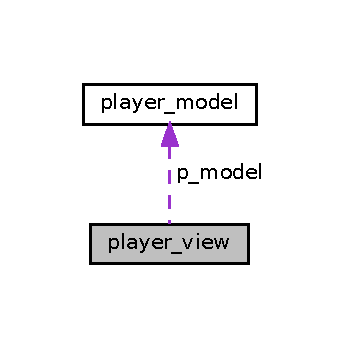
\includegraphics[width=168pt]{structplayer__view__coll__graph}
\end{center}
\end{figure}
\subsection*{Поля данных}
\begin{DoxyCompactItemize}
\item 
\hyperlink{structplayer__model}{player\+\_\+model} $\ast$ \hyperlink{structplayer__view_a8b8e41d687b369127d82d1271aca29ac}{p\+\_\+model}
\begin{DoxyCompactList}\small\item\em Адрес модели игрока. \end{DoxyCompactList}\item 
A\+L\+L\+E\+G\+R\+O\+\_\+\+B\+I\+T\+M\+AP $\ast$ \hyperlink{structplayer__view_adcfa5be54e3ef23cbd19acdcfef206c4}{p\+\_\+rect}
\begin{DoxyCompactList}\small\item\em Адрес прямоугольника, через который отображается игрока. \end{DoxyCompactList}\item 
unsigned int \hyperlink{structplayer__view_ae75fedba07d294d1f98716a0023641e6}{x\+\_\+start}
\begin{DoxyCompactList}\small\item\em Координата верхнего левого угла начальной позиции игрока по оси OX. \end{DoxyCompactList}\item 
unsigned int \hyperlink{structplayer__view_a35d236e445af2ed345f6b6147ea66aca}{y\+\_\+start}
\begin{DoxyCompactList}\small\item\em Координата верхнего левого угла начальной позиции игрока по оси OY. \end{DoxyCompactList}\item 
unsigned int \hyperlink{structplayer__view_ad5e7e7b6013080b75bb111b86634571d}{y\+\_\+finish}
\begin{DoxyCompactList}\small\item\em Координата верхнего левого угла конечно позиции игрока по оси OY. \end{DoxyCompactList}\end{DoxyCompactItemize}


\subsection{Подробное описание}
Структура, которая описывает отображение игрока. 

\subsection{Поля}
\mbox{\Hypertarget{structplayer__view_a8b8e41d687b369127d82d1271aca29ac}\label{structplayer__view_a8b8e41d687b369127d82d1271aca29ac}} 
\index{player\+\_\+view@{player\+\_\+view}!p\+\_\+model@{p\+\_\+model}}
\index{p\+\_\+model@{p\+\_\+model}!player\+\_\+view@{player\+\_\+view}}
\subsubsection{\texorpdfstring{p\+\_\+model}{p\_model}}
{\footnotesize\ttfamily \hyperlink{structplayer__model}{player\+\_\+model}$\ast$ player\+\_\+view\+::p\+\_\+model}



Адрес модели игрока. 

\mbox{\Hypertarget{structplayer__view_adcfa5be54e3ef23cbd19acdcfef206c4}\label{structplayer__view_adcfa5be54e3ef23cbd19acdcfef206c4}} 
\index{player\+\_\+view@{player\+\_\+view}!p\+\_\+rect@{p\+\_\+rect}}
\index{p\+\_\+rect@{p\+\_\+rect}!player\+\_\+view@{player\+\_\+view}}
\subsubsection{\texorpdfstring{p\+\_\+rect}{p\_rect}}
{\footnotesize\ttfamily A\+L\+L\+E\+G\+R\+O\+\_\+\+B\+I\+T\+M\+AP$\ast$ player\+\_\+view\+::p\+\_\+rect}



Адрес прямоугольника, через который отображается игрока. 

\mbox{\Hypertarget{structplayer__view_ae75fedba07d294d1f98716a0023641e6}\label{structplayer__view_ae75fedba07d294d1f98716a0023641e6}} 
\index{player\+\_\+view@{player\+\_\+view}!x\+\_\+start@{x\+\_\+start}}
\index{x\+\_\+start@{x\+\_\+start}!player\+\_\+view@{player\+\_\+view}}
\subsubsection{\texorpdfstring{x\+\_\+start}{x\_start}}
{\footnotesize\ttfamily unsigned int player\+\_\+view\+::x\+\_\+start}



Координата верхнего левого угла начальной позиции игрока по оси OX. 

\mbox{\Hypertarget{structplayer__view_ad5e7e7b6013080b75bb111b86634571d}\label{structplayer__view_ad5e7e7b6013080b75bb111b86634571d}} 
\index{player\+\_\+view@{player\+\_\+view}!y\+\_\+finish@{y\+\_\+finish}}
\index{y\+\_\+finish@{y\+\_\+finish}!player\+\_\+view@{player\+\_\+view}}
\subsubsection{\texorpdfstring{y\+\_\+finish}{y\_finish}}
{\footnotesize\ttfamily unsigned int player\+\_\+view\+::y\+\_\+finish}



Координата верхнего левого угла конечно позиции игрока по оси OY. 

\mbox{\Hypertarget{structplayer__view_a35d236e445af2ed345f6b6147ea66aca}\label{structplayer__view_a35d236e445af2ed345f6b6147ea66aca}} 
\index{player\+\_\+view@{player\+\_\+view}!y\+\_\+start@{y\+\_\+start}}
\index{y\+\_\+start@{y\+\_\+start}!player\+\_\+view@{player\+\_\+view}}
\subsubsection{\texorpdfstring{y\+\_\+start}{y\_start}}
{\footnotesize\ttfamily unsigned int player\+\_\+view\+::y\+\_\+start}



Координата верхнего левого угла начальной позиции игрока по оси OY. 



Объявления и описания членов структуры находятся в файле\+:\begin{DoxyCompactItemize}
\item 
src/\hyperlink{player__view_8h}{player\+\_\+view.\+h}\end{DoxyCompactItemize}

\hypertarget{structtimer__model}{}\section{Структура timer\+\_\+model}
\label{structtimer__model}\index{timer\+\_\+model@{timer\+\_\+model}}


Структура, которая описывает модель таймеров.  




{\ttfamily \#include $<$timer\+\_\+model.\+h$>$}

\subsection*{Поля данных}
\begin{DoxyCompactItemize}
\item 
char \hyperlink{structtimer__model_a02202197b7b11c2d3dde956d875a4c02}{top\+\_\+time} \mbox{[}\hyperlink{timer__model_8h_afb8e0513b4926ca94b38be5d60aaf125}{S\+I\+Z\+E\+\_\+\+T\+I\+M\+E\+\_\+\+S\+T\+R\+I\+NG}\mbox{]}
\begin{DoxyCompactList}\small\item\em Рекорное время. \end{DoxyCompactList}\item 
char \hyperlink{structtimer__model_afe9b325627d97aacb3c7952a788b003f}{current\+\_\+time} \mbox{[}\hyperlink{timer__model_8h_afb8e0513b4926ca94b38be5d60aaf125}{S\+I\+Z\+E\+\_\+\+T\+I\+M\+E\+\_\+\+S\+T\+R\+I\+NG}\mbox{]}
\begin{DoxyCompactList}\small\item\em Текущее время. \end{DoxyCompactList}\item 
time\+\_\+t \hyperlink{structtimer__model_aa78e974af2e5cde082a081c24c7fafc4}{start\+\_\+time}
\begin{DoxyCompactList}\small\item\em Время пуска таймера. \end{DoxyCompactList}\end{DoxyCompactItemize}


\subsection{Подробное описание}
Структура, которая описывает модель таймеров. 

\subsection{Поля}
\mbox{\Hypertarget{structtimer__model_afe9b325627d97aacb3c7952a788b003f}\label{structtimer__model_afe9b325627d97aacb3c7952a788b003f}} 
\index{timer\+\_\+model@{timer\+\_\+model}!current\+\_\+time@{current\+\_\+time}}
\index{current\+\_\+time@{current\+\_\+time}!timer\+\_\+model@{timer\+\_\+model}}
\subsubsection{\texorpdfstring{current\+\_\+time}{current\_time}}
{\footnotesize\ttfamily char timer\+\_\+model\+::current\+\_\+time\mbox{[}\hyperlink{timer__model_8h_afb8e0513b4926ca94b38be5d60aaf125}{S\+I\+Z\+E\+\_\+\+T\+I\+M\+E\+\_\+\+S\+T\+R\+I\+NG}\mbox{]}}



Текущее время. 

\mbox{\Hypertarget{structtimer__model_aa78e974af2e5cde082a081c24c7fafc4}\label{structtimer__model_aa78e974af2e5cde082a081c24c7fafc4}} 
\index{timer\+\_\+model@{timer\+\_\+model}!start\+\_\+time@{start\+\_\+time}}
\index{start\+\_\+time@{start\+\_\+time}!timer\+\_\+model@{timer\+\_\+model}}
\subsubsection{\texorpdfstring{start\+\_\+time}{start\_time}}
{\footnotesize\ttfamily time\+\_\+t timer\+\_\+model\+::start\+\_\+time}



Время пуска таймера. 

\mbox{\Hypertarget{structtimer__model_a02202197b7b11c2d3dde956d875a4c02}\label{structtimer__model_a02202197b7b11c2d3dde956d875a4c02}} 
\index{timer\+\_\+model@{timer\+\_\+model}!top\+\_\+time@{top\+\_\+time}}
\index{top\+\_\+time@{top\+\_\+time}!timer\+\_\+model@{timer\+\_\+model}}
\subsubsection{\texorpdfstring{top\+\_\+time}{top\_time}}
{\footnotesize\ttfamily char timer\+\_\+model\+::top\+\_\+time\mbox{[}\hyperlink{timer__model_8h_afb8e0513b4926ca94b38be5d60aaf125}{S\+I\+Z\+E\+\_\+\+T\+I\+M\+E\+\_\+\+S\+T\+R\+I\+NG}\mbox{]}}



Рекорное время. 



Объявления и описания членов структуры находятся в файле\+:\begin{DoxyCompactItemize}
\item 
src/\hyperlink{timer__model_8h}{timer\+\_\+model.\+h}\end{DoxyCompactItemize}

\hypertarget{structtimer__view}{}\section{Структура timer\+\_\+view}
\label{structtimer__view}\index{timer\+\_\+view@{timer\+\_\+view}}


Структура, которая описывает отображение таймеров.  




{\ttfamily \#include $<$timer\+\_\+view.\+h$>$}



Граф связей класса timer\+\_\+view\+:\nopagebreak
\begin{figure}[H]
\begin{center}
\leavevmode
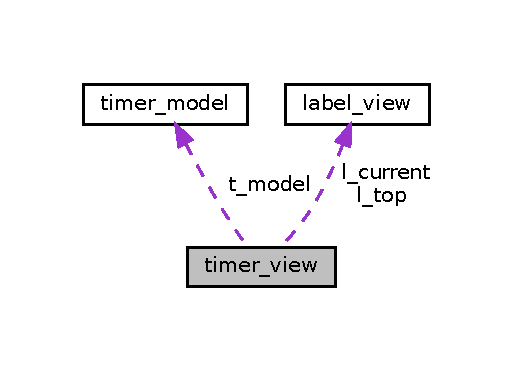
\includegraphics[width=247pt]{structtimer__view__coll__graph}
\end{center}
\end{figure}
\subsection*{Поля данных}
\begin{DoxyCompactItemize}
\item 
\hyperlink{structlabel__view}{label\+\_\+view} $\ast$ \hyperlink{structtimer__view_af1e48631c4b2eab39e49ac0ad7390b70}{l\+\_\+top}
\begin{DoxyCompactList}\small\item\em Адрес надписи с рекордным временем. \end{DoxyCompactList}\item 
\hyperlink{structlabel__view}{label\+\_\+view} $\ast$ \hyperlink{structtimer__view_a033b8a6e58675feb9c2c4b66fb56be9b}{l\+\_\+current}
\begin{DoxyCompactList}\small\item\em Адрес надписи с текущим временем. \end{DoxyCompactList}\item 
\hyperlink{structtimer__model}{timer\+\_\+model} $\ast$ \hyperlink{structtimer__view_a016f2b9a9c2d969b5a92f7d1a893bd3d}{t\+\_\+model}
\begin{DoxyCompactList}\small\item\em Адрес модели таймеров. \end{DoxyCompactList}\item 
unsigned int \hyperlink{structtimer__view_aae1b218e8d1526bd4abe54898de94a04}{shift\+\_\+x}
\begin{DoxyCompactList}\small\item\em Смещение позиций рисования таймеров по оси OX. \end{DoxyCompactList}\item 
unsigned int \hyperlink{structtimer__view_a52be0cc476c2242a46407d3d729ecbe4}{shift\+\_\+y}
\begin{DoxyCompactList}\small\item\em Смещение позиций рисования таймеров по оси OY. \end{DoxyCompactList}\end{DoxyCompactItemize}


\subsection{Подробное описание}
Структура, которая описывает отображение таймеров. 

\subsection{Поля}
\mbox{\Hypertarget{structtimer__view_a033b8a6e58675feb9c2c4b66fb56be9b}\label{structtimer__view_a033b8a6e58675feb9c2c4b66fb56be9b}} 
\index{timer\+\_\+view@{timer\+\_\+view}!l\+\_\+current@{l\+\_\+current}}
\index{l\+\_\+current@{l\+\_\+current}!timer\+\_\+view@{timer\+\_\+view}}
\subsubsection{\texorpdfstring{l\+\_\+current}{l\_current}}
{\footnotesize\ttfamily \hyperlink{structlabel__view}{label\+\_\+view}$\ast$ timer\+\_\+view\+::l\+\_\+current}



Адрес надписи с текущим временем. 

\mbox{\Hypertarget{structtimer__view_af1e48631c4b2eab39e49ac0ad7390b70}\label{structtimer__view_af1e48631c4b2eab39e49ac0ad7390b70}} 
\index{timer\+\_\+view@{timer\+\_\+view}!l\+\_\+top@{l\+\_\+top}}
\index{l\+\_\+top@{l\+\_\+top}!timer\+\_\+view@{timer\+\_\+view}}
\subsubsection{\texorpdfstring{l\+\_\+top}{l\_top}}
{\footnotesize\ttfamily \hyperlink{structlabel__view}{label\+\_\+view}$\ast$ timer\+\_\+view\+::l\+\_\+top}



Адрес надписи с рекордным временем. 

\mbox{\Hypertarget{structtimer__view_aae1b218e8d1526bd4abe54898de94a04}\label{structtimer__view_aae1b218e8d1526bd4abe54898de94a04}} 
\index{timer\+\_\+view@{timer\+\_\+view}!shift\+\_\+x@{shift\+\_\+x}}
\index{shift\+\_\+x@{shift\+\_\+x}!timer\+\_\+view@{timer\+\_\+view}}
\subsubsection{\texorpdfstring{shift\+\_\+x}{shift\_x}}
{\footnotesize\ttfamily unsigned int timer\+\_\+view\+::shift\+\_\+x}



Смещение позиций рисования таймеров по оси OX. 

\mbox{\Hypertarget{structtimer__view_a52be0cc476c2242a46407d3d729ecbe4}\label{structtimer__view_a52be0cc476c2242a46407d3d729ecbe4}} 
\index{timer\+\_\+view@{timer\+\_\+view}!shift\+\_\+y@{shift\+\_\+y}}
\index{shift\+\_\+y@{shift\+\_\+y}!timer\+\_\+view@{timer\+\_\+view}}
\subsubsection{\texorpdfstring{shift\+\_\+y}{shift\_y}}
{\footnotesize\ttfamily unsigned int timer\+\_\+view\+::shift\+\_\+y}



Смещение позиций рисования таймеров по оси OY. 

\mbox{\Hypertarget{structtimer__view_a016f2b9a9c2d969b5a92f7d1a893bd3d}\label{structtimer__view_a016f2b9a9c2d969b5a92f7d1a893bd3d}} 
\index{timer\+\_\+view@{timer\+\_\+view}!t\+\_\+model@{t\+\_\+model}}
\index{t\+\_\+model@{t\+\_\+model}!timer\+\_\+view@{timer\+\_\+view}}
\subsubsection{\texorpdfstring{t\+\_\+model}{t\_model}}
{\footnotesize\ttfamily \hyperlink{structtimer__model}{timer\+\_\+model}$\ast$ timer\+\_\+view\+::t\+\_\+model}



Адрес модели таймеров. 



Объявления и описания членов структуры находятся в файле\+:\begin{DoxyCompactItemize}
\item 
src/\hyperlink{timer__view_8h}{timer\+\_\+view.\+h}\end{DoxyCompactItemize}

\chapter{Файлы}
\hypertarget{_r_e_a_d_m_e_8md}{}\section{Файл R\+E\+A\+D\+M\+E.\+md}
\label{_r_e_a_d_m_e_8md}\index{R\+E\+A\+D\+M\+E.\+md@{R\+E\+A\+D\+M\+E.\+md}}

\hypertarget{error__report_8c}{}\section{Файл src/error\+\_\+report.c}
\label{error__report_8c}\index{src/error\+\_\+report.\+c@{src/error\+\_\+report.\+c}}


Файл, в котором реализованы функции логирования ошибок.  


{\ttfamily \#include \char`\"{}error\+\_\+report.\+h\char`\"{}}\newline
{\ttfamily \#include $<$stdio.\+h$>$}\newline
Граф включаемых заголовочных файлов для error\+\_\+report.\+c\+:\nopagebreak
\begin{figure}[H]
\begin{center}
\leavevmode
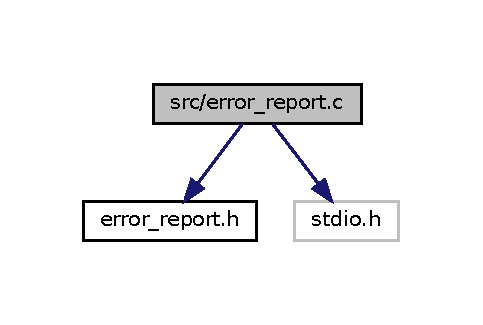
\includegraphics[width=232pt]{error__report_8c__incl}
\end{center}
\end{figure}
\subsection*{Функции}
\begin{DoxyCompactItemize}
\item 
void \hyperlink{error__report_8c_a1b4472f64c1bb3244ef7a031a0645ef9}{error\+\_\+report} (const char $\ast$fl\+\_\+name, const char $\ast$fn\+\_\+name, const char $\ast$mess)
\end{DoxyCompactItemize}


\subsection{Подробное описание}
Файл, в котором реализованы функции логирования ошибок. 



\subsection{Функции}
\mbox{\Hypertarget{error__report_8c_a1b4472f64c1bb3244ef7a031a0645ef9}\label{error__report_8c_a1b4472f64c1bb3244ef7a031a0645ef9}} 
\index{error\+\_\+report.\+c@{error\+\_\+report.\+c}!error\+\_\+report@{error\+\_\+report}}
\index{error\+\_\+report@{error\+\_\+report}!error\+\_\+report.\+c@{error\+\_\+report.\+c}}
\subsubsection{\texorpdfstring{error\+\_\+report()}{error\_report()}}
{\footnotesize\ttfamily void error\+\_\+report (\begin{DoxyParamCaption}\item[{const char $\ast$}]{fl\+\_\+name,  }\item[{const char $\ast$}]{fn\+\_\+name,  }\item[{const char $\ast$}]{mess }\end{DoxyParamCaption})}

Вывод сообщения об ошибки в поток stderr. 
\begin{DoxyParams}[1]{Аргументы}
\mbox{\tt in}  & {\em fl\+\_\+name} & -\/ имя файла, в котором возникла ошибка. \\
\hline
\mbox{\tt in}  & {\em fn\+\_\+name} & -\/ имя функции, в которой возникла ошибка. \\
\hline
\mbox{\tt in}  & {\em mess} & -\/ информационное сообщение, характеризующие ошибку. \\
\hline
\end{DoxyParams}

\hypertarget{error__report_8h}{}\section{Файл src/error\+\_\+report.h}
\label{error__report_8h}\index{src/error\+\_\+report.\+h@{src/error\+\_\+report.\+h}}


Файл, в котором опеределены функции логирования ошибок.  


Граф файлов, в которые включается этот файл\+:\nopagebreak
\begin{figure}[H]
\begin{center}
\leavevmode
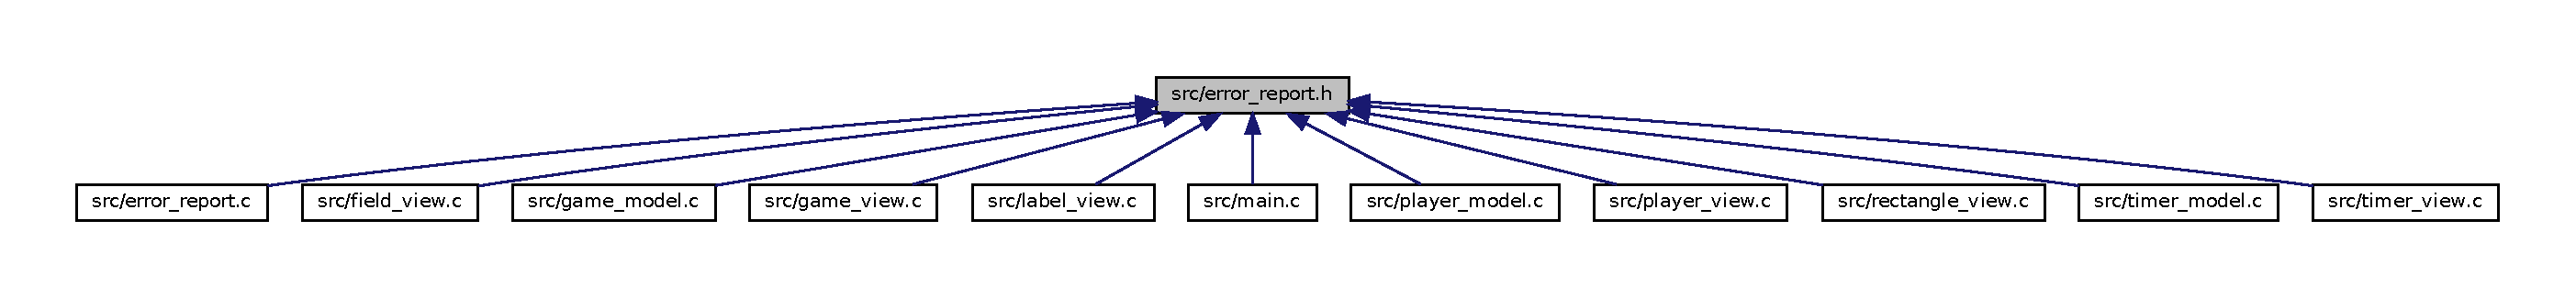
\includegraphics[width=350pt]{error__report_8h__dep__incl}
\end{center}
\end{figure}
\subsection*{Функции}
\begin{DoxyCompactItemize}
\item 
void \hyperlink{error__report_8h_a1b4472f64c1bb3244ef7a031a0645ef9}{error\+\_\+report} (const char $\ast$fl\+\_\+name, const char $\ast$fn\+\_\+name, const char $\ast$mess)
\end{DoxyCompactItemize}


\subsection{Подробное описание}
Файл, в котором опеределены функции логирования ошибок. 



\subsection{Функции}
\mbox{\Hypertarget{error__report_8h_a1b4472f64c1bb3244ef7a031a0645ef9}\label{error__report_8h_a1b4472f64c1bb3244ef7a031a0645ef9}} 
\index{error\+\_\+report.\+h@{error\+\_\+report.\+h}!error\+\_\+report@{error\+\_\+report}}
\index{error\+\_\+report@{error\+\_\+report}!error\+\_\+report.\+h@{error\+\_\+report.\+h}}
\subsubsection{\texorpdfstring{error\+\_\+report()}{error\_report()}}
{\footnotesize\ttfamily void error\+\_\+report (\begin{DoxyParamCaption}\item[{const char $\ast$}]{fl\+\_\+name,  }\item[{const char $\ast$}]{fn\+\_\+name,  }\item[{const char $\ast$}]{mess }\end{DoxyParamCaption})}

Вывод сообщения об ошибки в поток stderr. 
\begin{DoxyParams}[1]{Аргументы}
\mbox{\tt in}  & {\em fl\+\_\+name} & -\/ имя файла, в котором возникла ошибка. \\
\hline
\mbox{\tt in}  & {\em fn\+\_\+name} & -\/ имя функции, в которой возникла ошибка. \\
\hline
\mbox{\tt in}  & {\em mess} & -\/ информационное сообщение, характеризующие ошибку. \\
\hline
\end{DoxyParams}

\hypertarget{field__view_8c}{}\section{Файл src/field\+\_\+view.c}
\label{field__view_8c}\index{src/field\+\_\+view.\+c@{src/field\+\_\+view.\+c}}


Файл, в котором реализованы функции для работы с отображением игрового поля.  


{\ttfamily \#include \char`\"{}field\+\_\+view.\+h\char`\"{}}\newline
{\ttfamily \#include \char`\"{}rectangle\+\_\+view.\+h\char`\"{}}\newline
{\ttfamily \#include \char`\"{}error\+\_\+report.\+h\char`\"{}}\newline
{\ttfamily \#include $<$stdlib.\+h$>$}\newline
Граф включаемых заголовочных файлов для field\+\_\+view.\+c\+:\nopagebreak
\begin{figure}[H]
\begin{center}
\leavevmode
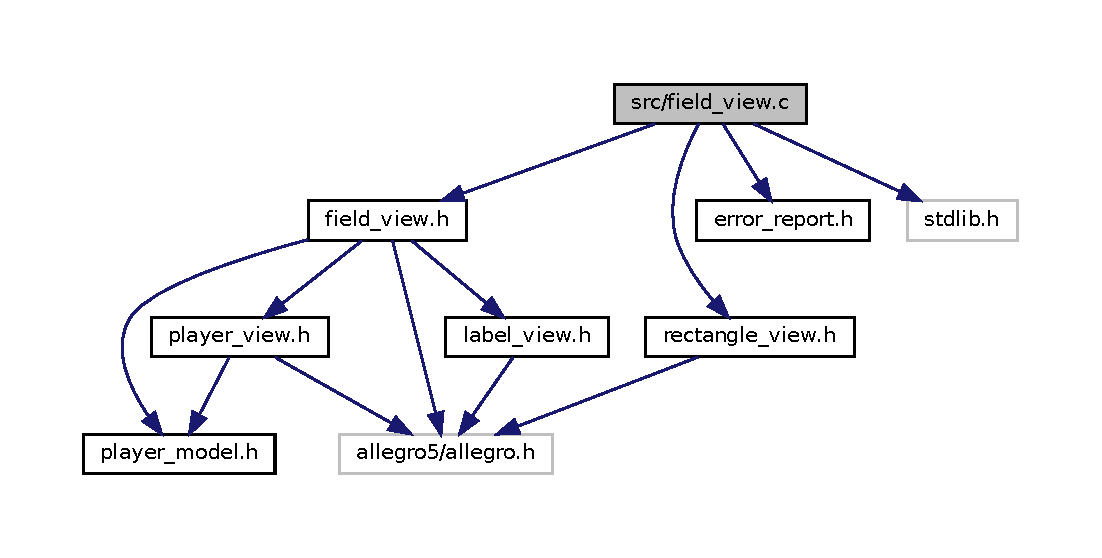
\includegraphics[width=350pt]{field__view_8c__incl}
\end{center}
\end{figure}
\subsection*{Макросы}
\begin{DoxyCompactItemize}
\item 
\#define \hyperlink{field__view_8c_ab117546549783a058d0321a287699579}{F\+I\+L\+E\+\_\+\+N\+A\+ME}~\char`\"{}field\+\_\+view.\+c\char`\"{}
\begin{DoxyCompactList}\small\item\em Текущие имя файла. \end{DoxyCompactList}\item 
\#define \hyperlink{field__view_8c_aba64ab31ac50908f7aa4125955fcf2ed}{F\+U\+N\+\_\+\+N\+A\+ME}~\char`\"{}field\+\_\+view\+\_\+create\char`\"{}
\begin{DoxyCompactList}\small\item\em Имя текущей функции. \end{DoxyCompactList}\item 
\#define \hyperlink{field__view_8c_aba64ab31ac50908f7aa4125955fcf2ed}{F\+U\+N\+\_\+\+N\+A\+ME}~\char`\"{}field\+\_\+view\+\_\+draw\char`\"{}
\begin{DoxyCompactList}\small\item\em Имя текущей функции. \end{DoxyCompactList}\item 
\#define \hyperlink{field__view_8c_aba64ab31ac50908f7aa4125955fcf2ed}{F\+U\+N\+\_\+\+N\+A\+ME}~\char`\"{}field\+\_\+view\+\_\+destroy\char`\"{}
\begin{DoxyCompactList}\small\item\em Имя текущей функции. \end{DoxyCompactList}\end{DoxyCompactItemize}
\subsection*{Функции}
\begin{DoxyCompactItemize}
\item 
\hyperlink{structfield__view}{field\+\_\+view} $\ast$ \hyperlink{field__view_8c_a21ada3aca6c3fffd7ebc7b12776cf443}{field\+\_\+view\+\_\+create} (\hyperlink{structplayer__model}{player\+\_\+model} $\ast$p\+\_\+model, unsigned int width, unsigned int height)
\item 
int \hyperlink{field__view_8c_a44aa3af68e8a6b237018bfe7cfb70c33}{field\+\_\+view\+\_\+draw} (\hyperlink{structfield__view}{field\+\_\+view} $\ast$f\+\_\+view)
\item 
int \hyperlink{field__view_8c_a3b5569e6513c7010fd537ea62876309f}{field\+\_\+view\+\_\+destroy} (\hyperlink{structfield__view}{field\+\_\+view} $\ast$f\+\_\+view)
\end{DoxyCompactItemize}


\subsection{Подробное описание}
Файл, в котором реализованы функции для работы с отображением игрового поля. 



\subsection{Макросы}
\mbox{\Hypertarget{field__view_8c_ab117546549783a058d0321a287699579}\label{field__view_8c_ab117546549783a058d0321a287699579}} 
\index{field\+\_\+view.\+c@{field\+\_\+view.\+c}!F\+I\+L\+E\+\_\+\+N\+A\+ME@{F\+I\+L\+E\+\_\+\+N\+A\+ME}}
\index{F\+I\+L\+E\+\_\+\+N\+A\+ME@{F\+I\+L\+E\+\_\+\+N\+A\+ME}!field\+\_\+view.\+c@{field\+\_\+view.\+c}}
\subsubsection{\texorpdfstring{F\+I\+L\+E\+\_\+\+N\+A\+ME}{FILE\_NAME}}
{\footnotesize\ttfamily \#define F\+I\+L\+E\+\_\+\+N\+A\+ME~\char`\"{}field\+\_\+view.\+c\char`\"{}}



Текущие имя файла. 

\mbox{\Hypertarget{field__view_8c_aba64ab31ac50908f7aa4125955fcf2ed}\label{field__view_8c_aba64ab31ac50908f7aa4125955fcf2ed}} 
\index{field\+\_\+view.\+c@{field\+\_\+view.\+c}!F\+U\+N\+\_\+\+N\+A\+ME@{F\+U\+N\+\_\+\+N\+A\+ME}}
\index{F\+U\+N\+\_\+\+N\+A\+ME@{F\+U\+N\+\_\+\+N\+A\+ME}!field\+\_\+view.\+c@{field\+\_\+view.\+c}}
\subsubsection{\texorpdfstring{F\+U\+N\+\_\+\+N\+A\+ME}{FUN\_NAME}\hspace{0.1cm}{\footnotesize\ttfamily [1/3]}}
{\footnotesize\ttfamily \#define F\+U\+N\+\_\+\+N\+A\+ME~\char`\"{}field\+\_\+view\+\_\+create\char`\"{}}



Имя текущей функции. 

\mbox{\Hypertarget{field__view_8c_aba64ab31ac50908f7aa4125955fcf2ed}\label{field__view_8c_aba64ab31ac50908f7aa4125955fcf2ed}} 
\index{field\+\_\+view.\+c@{field\+\_\+view.\+c}!F\+U\+N\+\_\+\+N\+A\+ME@{F\+U\+N\+\_\+\+N\+A\+ME}}
\index{F\+U\+N\+\_\+\+N\+A\+ME@{F\+U\+N\+\_\+\+N\+A\+ME}!field\+\_\+view.\+c@{field\+\_\+view.\+c}}
\subsubsection{\texorpdfstring{F\+U\+N\+\_\+\+N\+A\+ME}{FUN\_NAME}\hspace{0.1cm}{\footnotesize\ttfamily [2/3]}}
{\footnotesize\ttfamily \#define F\+U\+N\+\_\+\+N\+A\+ME~\char`\"{}field\+\_\+view\+\_\+draw\char`\"{}}



Имя текущей функции. 

\mbox{\Hypertarget{field__view_8c_aba64ab31ac50908f7aa4125955fcf2ed}\label{field__view_8c_aba64ab31ac50908f7aa4125955fcf2ed}} 
\index{field\+\_\+view.\+c@{field\+\_\+view.\+c}!F\+U\+N\+\_\+\+N\+A\+ME@{F\+U\+N\+\_\+\+N\+A\+ME}}
\index{F\+U\+N\+\_\+\+N\+A\+ME@{F\+U\+N\+\_\+\+N\+A\+ME}!field\+\_\+view.\+c@{field\+\_\+view.\+c}}
\subsubsection{\texorpdfstring{F\+U\+N\+\_\+\+N\+A\+ME}{FUN\_NAME}\hspace{0.1cm}{\footnotesize\ttfamily [3/3]}}
{\footnotesize\ttfamily \#define F\+U\+N\+\_\+\+N\+A\+ME~\char`\"{}field\+\_\+view\+\_\+destroy\char`\"{}}



Имя текущей функции. 



\subsection{Функции}
\mbox{\Hypertarget{field__view_8c_a21ada3aca6c3fffd7ebc7b12776cf443}\label{field__view_8c_a21ada3aca6c3fffd7ebc7b12776cf443}} 
\index{field\+\_\+view.\+c@{field\+\_\+view.\+c}!field\+\_\+view\+\_\+create@{field\+\_\+view\+\_\+create}}
\index{field\+\_\+view\+\_\+create@{field\+\_\+view\+\_\+create}!field\+\_\+view.\+c@{field\+\_\+view.\+c}}
\subsubsection{\texorpdfstring{field\+\_\+view\+\_\+create()}{field\_view\_create()}}
{\footnotesize\ttfamily \hyperlink{structfield__view}{field\+\_\+view}$\ast$ field\+\_\+view\+\_\+create (\begin{DoxyParamCaption}\item[{\hyperlink{structplayer__model}{player\+\_\+model} $\ast$}]{p\+\_\+model,  }\item[{unsigned int}]{width,  }\item[{unsigned int}]{height }\end{DoxyParamCaption})}

Создание отображения игрового поля. 
\begin{DoxyParams}[1]{Аргументы}
\mbox{\tt in}  & {\em p\+\_\+model} & -\/ модель игрока. \\
\hline
\mbox{\tt in}  & {\em width} & -\/ ширина поля. \\
\hline
\mbox{\tt in}  & {\em height} & -\/ высота поля. \\
\hline
\end{DoxyParams}
\begin{DoxyReturn}{Возвращает}
Адрес, созданного отображения игрового поля. ~\newline
 N\+U\+LL, если во время создания отображения игрового поля произошла ошибка. 
\end{DoxyReturn}
\mbox{\Hypertarget{field__view_8c_a3b5569e6513c7010fd537ea62876309f}\label{field__view_8c_a3b5569e6513c7010fd537ea62876309f}} 
\index{field\+\_\+view.\+c@{field\+\_\+view.\+c}!field\+\_\+view\+\_\+destroy@{field\+\_\+view\+\_\+destroy}}
\index{field\+\_\+view\+\_\+destroy@{field\+\_\+view\+\_\+destroy}!field\+\_\+view.\+c@{field\+\_\+view.\+c}}
\subsubsection{\texorpdfstring{field\+\_\+view\+\_\+destroy()}{field\_view\_destroy()}}
{\footnotesize\ttfamily int field\+\_\+view\+\_\+destroy (\begin{DoxyParamCaption}\item[{\hyperlink{structfield__view}{field\+\_\+view} $\ast$}]{f\+\_\+view }\end{DoxyParamCaption})}

Удаление отображения игрового поля. 
\begin{DoxyParams}[1]{Аргументы}
\mbox{\tt in}  & {\em f\+\_\+view} & -\/ адрес отображения игрового поля, которое нужно удалить. \\
\hline
\end{DoxyParams}
\begin{DoxyReturn}{Возвращает}
Ноль, если удаление прошло успешно. ~\newline
 Ненулевое число, если во время удаления произошла ошибка. 
\end{DoxyReturn}
\mbox{\Hypertarget{field__view_8c_a44aa3af68e8a6b237018bfe7cfb70c33}\label{field__view_8c_a44aa3af68e8a6b237018bfe7cfb70c33}} 
\index{field\+\_\+view.\+c@{field\+\_\+view.\+c}!field\+\_\+view\+\_\+draw@{field\+\_\+view\+\_\+draw}}
\index{field\+\_\+view\+\_\+draw@{field\+\_\+view\+\_\+draw}!field\+\_\+view.\+c@{field\+\_\+view.\+c}}
\subsubsection{\texorpdfstring{field\+\_\+view\+\_\+draw()}{field\_view\_draw()}}
{\footnotesize\ttfamily int field\+\_\+view\+\_\+draw (\begin{DoxyParamCaption}\item[{\hyperlink{structfield__view}{field\+\_\+view} $\ast$}]{f\+\_\+view }\end{DoxyParamCaption})}

Рисование отображения игрового поля. 
\begin{DoxyParams}[1]{Аргументы}
\mbox{\tt in}  & {\em f\+\_\+view} & -\/ адрес отображения игрового, которое нужно нарисовать. \\
\hline
\end{DoxyParams}
\begin{DoxyReturn}{Возвращает}
Ноль, если отображение было успешно отрисовано. ~\newline
 Ненулевое число, если во время рисования произошла ошибка. 
\end{DoxyReturn}

\hypertarget{field__view_8h}{}\section{Файл src/field\+\_\+view.h}
\label{field__view_8h}\index{src/field\+\_\+view.\+h@{src/field\+\_\+view.\+h}}


Файл, в котором опеределены функции для работы с отображением игрового поля.  


{\ttfamily \#include \char`\"{}player\+\_\+model.\+h\char`\"{}}\newline
{\ttfamily \#include \char`\"{}player\+\_\+view.\+h\char`\"{}}\newline
{\ttfamily \#include \char`\"{}label\+\_\+view.\+h\char`\"{}}\newline
{\ttfamily \#include $<$allegro5/allegro.\+h$>$}\newline
Граф включаемых заголовочных файлов для field\+\_\+view.\+h\+:\nopagebreak
\begin{figure}[H]
\begin{center}
\leavevmode
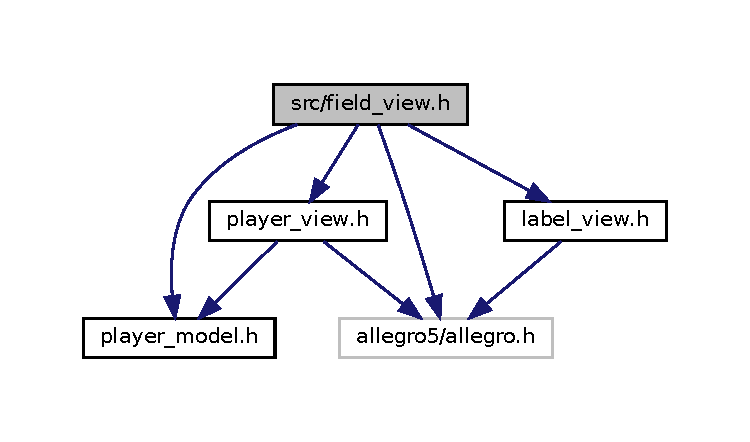
\includegraphics[width=350pt]{field__view_8h__incl}
\end{center}
\end{figure}
Граф файлов, в которые включается этот файл\+:\nopagebreak
\begin{figure}[H]
\begin{center}
\leavevmode
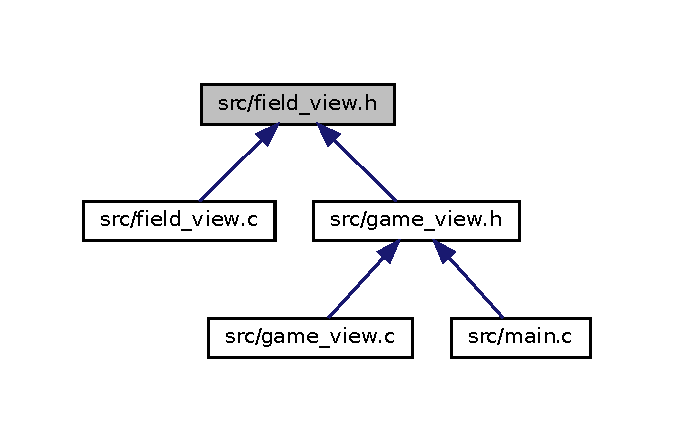
\includegraphics[width=324pt]{field__view_8h__dep__incl}
\end{center}
\end{figure}
\subsection*{Структуры данных}
\begin{DoxyCompactItemize}
\item 
struct \hyperlink{structfield__view}{field\+\_\+view}
\begin{DoxyCompactList}\small\item\em Структура, которая описывает отображение игрового поля. \end{DoxyCompactList}\end{DoxyCompactItemize}
\subsection*{Макросы}
\begin{DoxyCompactItemize}
\item 
\#define \hyperlink{field__view_8h_aec9655085e48e4fda789531146e9f1d0}{F\+I\+E\+L\+D\+\_\+\+B\+O\+R\+D\+E\+R\+\_\+\+S\+I\+ZE}~10
\begin{DoxyCompactList}\small\item\em Размер рамки. \end{DoxyCompactList}\item 
\#define \hyperlink{field__view_8h_ac8b40aa2e97ca893d0e2b289bcb47b71}{F\+I\+E\+L\+D\+\_\+\+H\+E\+G\+I\+H\+T\+\_\+\+F\+I\+N\+I\+SH}~70
\begin{DoxyCompactList}\small\item\em Высота надписи \char`\"{}\+Finish\char`\"{}. \end{DoxyCompactList}\item 
\#define \hyperlink{field__view_8h_acd7c051921458cc9c3a5ee750df2b0c3}{F\+I\+E\+L\+D\+\_\+\+B\+O\+R\+D\+E\+R\+\_\+\+C\+O\+L\+OR}~al\+\_\+map\+\_\+rgb(0, 0, 0)
\begin{DoxyCompactList}\small\item\em Цвет рамки. \end{DoxyCompactList}\item 
\#define \hyperlink{field__view_8h_a8a09f9e515afb676c783bb01e3a058f4}{F\+I\+E\+L\+D\+\_\+\+B\+A\+C\+K\+G\+R\+O\+U\+N\+D\+\_\+\+C\+O\+L\+OR}~al\+\_\+map\+\_\+rgb(255, 255, 255)
\begin{DoxyCompactList}\small\item\em Цвет фона. \end{DoxyCompactList}\item 
\#define \hyperlink{field__view_8h_ac7574d320ad8df89f500dedecb681b41}{F\+I\+E\+L\+D\+\_\+\+F\+I\+N\+I\+S\+H\+\_\+\+C\+O\+L\+OR}~al\+\_\+map\+\_\+rgb(255, 99, 71)
\begin{DoxyCompactList}\small\item\em Цвет надписи \char`\"{}\+Finish\char`\"{}. \end{DoxyCompactList}\end{DoxyCompactItemize}
\subsection*{Определения типов}
\begin{DoxyCompactItemize}
\item 
typedef struct \hyperlink{structfield__view}{field\+\_\+view} \hyperlink{field__view_8h_ae82b096186d36dc129037b5d35937f88}{field\+\_\+view}
\end{DoxyCompactItemize}
\subsection*{Функции}
\begin{DoxyCompactItemize}
\item 
\hyperlink{structfield__view}{field\+\_\+view} $\ast$ \hyperlink{field__view_8h_a21ada3aca6c3fffd7ebc7b12776cf443}{field\+\_\+view\+\_\+create} (\hyperlink{structplayer__model}{player\+\_\+model} $\ast$p\+\_\+model, unsigned int width, unsigned int height)
\item 
int \hyperlink{field__view_8h_a44aa3af68e8a6b237018bfe7cfb70c33}{field\+\_\+view\+\_\+draw} (\hyperlink{structfield__view}{field\+\_\+view} $\ast$f\+\_\+view)
\item 
int \hyperlink{field__view_8h_a3b5569e6513c7010fd537ea62876309f}{field\+\_\+view\+\_\+destroy} (\hyperlink{structfield__view}{field\+\_\+view} $\ast$f\+\_\+view)
\end{DoxyCompactItemize}


\subsection{Подробное описание}
Файл, в котором опеределены функции для работы с отображением игрового поля. 



\subsection{Макросы}
\mbox{\Hypertarget{field__view_8h_a8a09f9e515afb676c783bb01e3a058f4}\label{field__view_8h_a8a09f9e515afb676c783bb01e3a058f4}} 
\index{field\+\_\+view.\+h@{field\+\_\+view.\+h}!F\+I\+E\+L\+D\+\_\+\+B\+A\+C\+K\+G\+R\+O\+U\+N\+D\+\_\+\+C\+O\+L\+OR@{F\+I\+E\+L\+D\+\_\+\+B\+A\+C\+K\+G\+R\+O\+U\+N\+D\+\_\+\+C\+O\+L\+OR}}
\index{F\+I\+E\+L\+D\+\_\+\+B\+A\+C\+K\+G\+R\+O\+U\+N\+D\+\_\+\+C\+O\+L\+OR@{F\+I\+E\+L\+D\+\_\+\+B\+A\+C\+K\+G\+R\+O\+U\+N\+D\+\_\+\+C\+O\+L\+OR}!field\+\_\+view.\+h@{field\+\_\+view.\+h}}
\subsubsection{\texorpdfstring{F\+I\+E\+L\+D\+\_\+\+B\+A\+C\+K\+G\+R\+O\+U\+N\+D\+\_\+\+C\+O\+L\+OR}{FIELD\_BACKGROUND\_COLOR}}
{\footnotesize\ttfamily \#define F\+I\+E\+L\+D\+\_\+\+B\+A\+C\+K\+G\+R\+O\+U\+N\+D\+\_\+\+C\+O\+L\+OR~al\+\_\+map\+\_\+rgb(255, 255, 255)}



Цвет фона. 

\mbox{\Hypertarget{field__view_8h_acd7c051921458cc9c3a5ee750df2b0c3}\label{field__view_8h_acd7c051921458cc9c3a5ee750df2b0c3}} 
\index{field\+\_\+view.\+h@{field\+\_\+view.\+h}!F\+I\+E\+L\+D\+\_\+\+B\+O\+R\+D\+E\+R\+\_\+\+C\+O\+L\+OR@{F\+I\+E\+L\+D\+\_\+\+B\+O\+R\+D\+E\+R\+\_\+\+C\+O\+L\+OR}}
\index{F\+I\+E\+L\+D\+\_\+\+B\+O\+R\+D\+E\+R\+\_\+\+C\+O\+L\+OR@{F\+I\+E\+L\+D\+\_\+\+B\+O\+R\+D\+E\+R\+\_\+\+C\+O\+L\+OR}!field\+\_\+view.\+h@{field\+\_\+view.\+h}}
\subsubsection{\texorpdfstring{F\+I\+E\+L\+D\+\_\+\+B\+O\+R\+D\+E\+R\+\_\+\+C\+O\+L\+OR}{FIELD\_BORDER\_COLOR}}
{\footnotesize\ttfamily \#define F\+I\+E\+L\+D\+\_\+\+B\+O\+R\+D\+E\+R\+\_\+\+C\+O\+L\+OR~al\+\_\+map\+\_\+rgb(0, 0, 0)}



Цвет рамки. 

\mbox{\Hypertarget{field__view_8h_aec9655085e48e4fda789531146e9f1d0}\label{field__view_8h_aec9655085e48e4fda789531146e9f1d0}} 
\index{field\+\_\+view.\+h@{field\+\_\+view.\+h}!F\+I\+E\+L\+D\+\_\+\+B\+O\+R\+D\+E\+R\+\_\+\+S\+I\+ZE@{F\+I\+E\+L\+D\+\_\+\+B\+O\+R\+D\+E\+R\+\_\+\+S\+I\+ZE}}
\index{F\+I\+E\+L\+D\+\_\+\+B\+O\+R\+D\+E\+R\+\_\+\+S\+I\+ZE@{F\+I\+E\+L\+D\+\_\+\+B\+O\+R\+D\+E\+R\+\_\+\+S\+I\+ZE}!field\+\_\+view.\+h@{field\+\_\+view.\+h}}
\subsubsection{\texorpdfstring{F\+I\+E\+L\+D\+\_\+\+B\+O\+R\+D\+E\+R\+\_\+\+S\+I\+ZE}{FIELD\_BORDER\_SIZE}}
{\footnotesize\ttfamily \#define F\+I\+E\+L\+D\+\_\+\+B\+O\+R\+D\+E\+R\+\_\+\+S\+I\+ZE~10}



Размер рамки. 

\mbox{\Hypertarget{field__view_8h_ac7574d320ad8df89f500dedecb681b41}\label{field__view_8h_ac7574d320ad8df89f500dedecb681b41}} 
\index{field\+\_\+view.\+h@{field\+\_\+view.\+h}!F\+I\+E\+L\+D\+\_\+\+F\+I\+N\+I\+S\+H\+\_\+\+C\+O\+L\+OR@{F\+I\+E\+L\+D\+\_\+\+F\+I\+N\+I\+S\+H\+\_\+\+C\+O\+L\+OR}}
\index{F\+I\+E\+L\+D\+\_\+\+F\+I\+N\+I\+S\+H\+\_\+\+C\+O\+L\+OR@{F\+I\+E\+L\+D\+\_\+\+F\+I\+N\+I\+S\+H\+\_\+\+C\+O\+L\+OR}!field\+\_\+view.\+h@{field\+\_\+view.\+h}}
\subsubsection{\texorpdfstring{F\+I\+E\+L\+D\+\_\+\+F\+I\+N\+I\+S\+H\+\_\+\+C\+O\+L\+OR}{FIELD\_FINISH\_COLOR}}
{\footnotesize\ttfamily \#define F\+I\+E\+L\+D\+\_\+\+F\+I\+N\+I\+S\+H\+\_\+\+C\+O\+L\+OR~al\+\_\+map\+\_\+rgb(255, 99, 71)}



Цвет надписи \char`\"{}\+Finish\char`\"{}. 

\mbox{\Hypertarget{field__view_8h_ac8b40aa2e97ca893d0e2b289bcb47b71}\label{field__view_8h_ac8b40aa2e97ca893d0e2b289bcb47b71}} 
\index{field\+\_\+view.\+h@{field\+\_\+view.\+h}!F\+I\+E\+L\+D\+\_\+\+H\+E\+G\+I\+H\+T\+\_\+\+F\+I\+N\+I\+SH@{F\+I\+E\+L\+D\+\_\+\+H\+E\+G\+I\+H\+T\+\_\+\+F\+I\+N\+I\+SH}}
\index{F\+I\+E\+L\+D\+\_\+\+H\+E\+G\+I\+H\+T\+\_\+\+F\+I\+N\+I\+SH@{F\+I\+E\+L\+D\+\_\+\+H\+E\+G\+I\+H\+T\+\_\+\+F\+I\+N\+I\+SH}!field\+\_\+view.\+h@{field\+\_\+view.\+h}}
\subsubsection{\texorpdfstring{F\+I\+E\+L\+D\+\_\+\+H\+E\+G\+I\+H\+T\+\_\+\+F\+I\+N\+I\+SH}{FIELD\_HEGIHT\_FINISH}}
{\footnotesize\ttfamily \#define F\+I\+E\+L\+D\+\_\+\+H\+E\+G\+I\+H\+T\+\_\+\+F\+I\+N\+I\+SH~70}



Высота надписи \char`\"{}\+Finish\char`\"{}. 



\subsection{Типы}
\mbox{\Hypertarget{field__view_8h_ae82b096186d36dc129037b5d35937f88}\label{field__view_8h_ae82b096186d36dc129037b5d35937f88}} 
\index{field\+\_\+view.\+h@{field\+\_\+view.\+h}!field\+\_\+view@{field\+\_\+view}}
\index{field\+\_\+view@{field\+\_\+view}!field\+\_\+view.\+h@{field\+\_\+view.\+h}}
\subsubsection{\texorpdfstring{field\+\_\+view}{field\_view}}
{\footnotesize\ttfamily typedef struct \hyperlink{structfield__view}{field\+\_\+view} \hyperlink{structfield__view}{field\+\_\+view}}



\subsection{Функции}
\mbox{\Hypertarget{field__view_8h_a21ada3aca6c3fffd7ebc7b12776cf443}\label{field__view_8h_a21ada3aca6c3fffd7ebc7b12776cf443}} 
\index{field\+\_\+view.\+h@{field\+\_\+view.\+h}!field\+\_\+view\+\_\+create@{field\+\_\+view\+\_\+create}}
\index{field\+\_\+view\+\_\+create@{field\+\_\+view\+\_\+create}!field\+\_\+view.\+h@{field\+\_\+view.\+h}}
\subsubsection{\texorpdfstring{field\+\_\+view\+\_\+create()}{field\_view\_create()}}
{\footnotesize\ttfamily \hyperlink{structfield__view}{field\+\_\+view}$\ast$ field\+\_\+view\+\_\+create (\begin{DoxyParamCaption}\item[{\hyperlink{structplayer__model}{player\+\_\+model} $\ast$}]{p\+\_\+model,  }\item[{unsigned int}]{width,  }\item[{unsigned int}]{height }\end{DoxyParamCaption})}

Создание отображения игрового поля. 
\begin{DoxyParams}[1]{Аргументы}
\mbox{\tt in}  & {\em p\+\_\+model} & -\/ модель игрока. \\
\hline
\mbox{\tt in}  & {\em width} & -\/ ширина поля. \\
\hline
\mbox{\tt in}  & {\em height} & -\/ высота поля. \\
\hline
\end{DoxyParams}
\begin{DoxyReturn}{Возвращает}
Адрес, созданного отображения игрового поля. ~\newline
 N\+U\+LL, если во время создания отображения игрового поля произошла ошибка. 
\end{DoxyReturn}
\mbox{\Hypertarget{field__view_8h_a3b5569e6513c7010fd537ea62876309f}\label{field__view_8h_a3b5569e6513c7010fd537ea62876309f}} 
\index{field\+\_\+view.\+h@{field\+\_\+view.\+h}!field\+\_\+view\+\_\+destroy@{field\+\_\+view\+\_\+destroy}}
\index{field\+\_\+view\+\_\+destroy@{field\+\_\+view\+\_\+destroy}!field\+\_\+view.\+h@{field\+\_\+view.\+h}}
\subsubsection{\texorpdfstring{field\+\_\+view\+\_\+destroy()}{field\_view\_destroy()}}
{\footnotesize\ttfamily int field\+\_\+view\+\_\+destroy (\begin{DoxyParamCaption}\item[{\hyperlink{structfield__view}{field\+\_\+view} $\ast$}]{f\+\_\+view }\end{DoxyParamCaption})}

Удаление отображения игрового поля. 
\begin{DoxyParams}[1]{Аргументы}
\mbox{\tt in}  & {\em f\+\_\+view} & -\/ адрес отображения игрового поля, которое нужно удалить. \\
\hline
\end{DoxyParams}
\begin{DoxyReturn}{Возвращает}
Ноль, если удаление прошло успешно. ~\newline
 Ненулевое число, если во время удаления произошла ошибка. 
\end{DoxyReturn}
\mbox{\Hypertarget{field__view_8h_a44aa3af68e8a6b237018bfe7cfb70c33}\label{field__view_8h_a44aa3af68e8a6b237018bfe7cfb70c33}} 
\index{field\+\_\+view.\+h@{field\+\_\+view.\+h}!field\+\_\+view\+\_\+draw@{field\+\_\+view\+\_\+draw}}
\index{field\+\_\+view\+\_\+draw@{field\+\_\+view\+\_\+draw}!field\+\_\+view.\+h@{field\+\_\+view.\+h}}
\subsubsection{\texorpdfstring{field\+\_\+view\+\_\+draw()}{field\_view\_draw()}}
{\footnotesize\ttfamily int field\+\_\+view\+\_\+draw (\begin{DoxyParamCaption}\item[{\hyperlink{structfield__view}{field\+\_\+view} $\ast$}]{f\+\_\+view }\end{DoxyParamCaption})}

Рисование отображения игрового поля. 
\begin{DoxyParams}[1]{Аргументы}
\mbox{\tt in}  & {\em f\+\_\+view} & -\/ адрес отображения игрового, которое нужно нарисовать. \\
\hline
\end{DoxyParams}
\begin{DoxyReturn}{Возвращает}
Ноль, если отображение было успешно отрисовано. ~\newline
 Ненулевое число, если во время рисования произошла ошибка. 
\end{DoxyReturn}

\hypertarget{game__model_8c}{}\section{Файл src/game\+\_\+model.c}
\label{game__model_8c}\index{src/game\+\_\+model.\+c@{src/game\+\_\+model.\+c}}
{\ttfamily \#include \char`\"{}game\+\_\+model.\+h\char`\"{}}\newline
{\ttfamily \#include \char`\"{}error\+\_\+report.\+h\char`\"{}}\newline
{\ttfamily \#include $<$stdlib.\+h$>$}\newline
{\ttfamily \#include $<$math.\+h$>$}\newline
{\ttfamily \#include $<$stdbool.\+h$>$}\newline
Граф включаемых заголовочных файлов для game\+\_\+model.\+c\+:\nopagebreak
\begin{figure}[H]
\begin{center}
\leavevmode
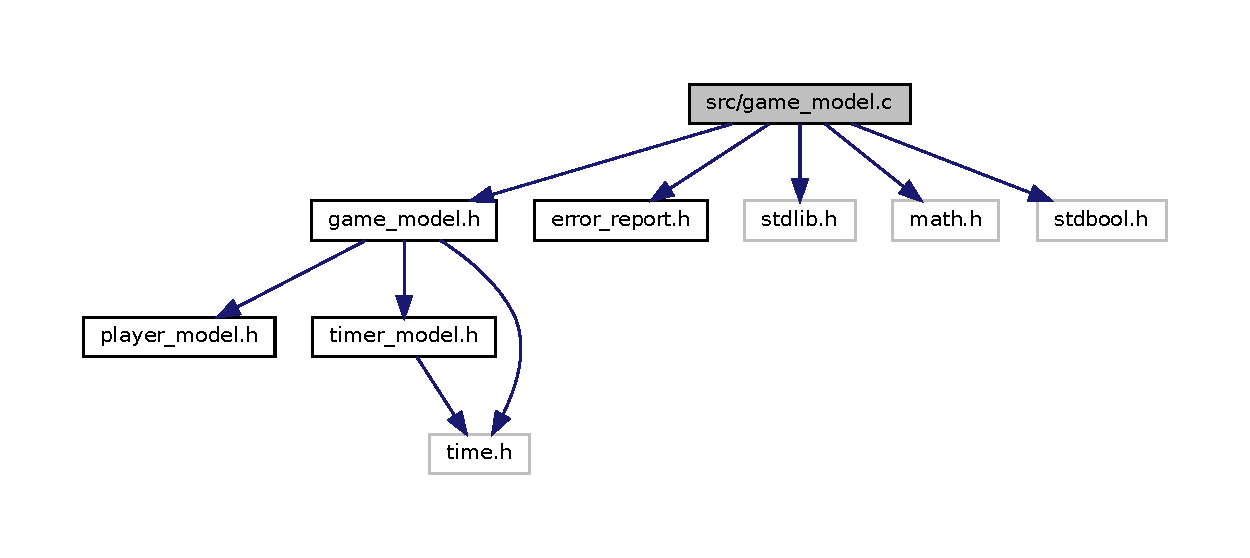
\includegraphics[width=350pt]{game__model_8c__incl}
\end{center}
\end{figure}
\subsection*{Макросы}
\begin{DoxyCompactItemize}
\item 
\#define \hyperlink{game__model_8c_ab117546549783a058d0321a287699579}{F\+I\+L\+E\+\_\+\+N\+A\+ME}~\char`\"{}game\+\_\+model.\+c\char`\"{}
\begin{DoxyCompactList}\small\item\em Имя текущего файла. \end{DoxyCompactList}\item 
\#define \hyperlink{game__model_8c_aba64ab31ac50908f7aa4125955fcf2ed}{F\+U\+N\+\_\+\+N\+A\+ME}~\char`\"{}game\+\_\+model\+\_\+create\char`\"{}
\begin{DoxyCompactList}\small\item\em Имя текущей функции. \end{DoxyCompactList}\item 
\#define \hyperlink{game__model_8c_aba64ab31ac50908f7aa4125955fcf2ed}{F\+U\+N\+\_\+\+N\+A\+ME}~\char`\"{}game\+\_\+model\+\_\+key\+\_\+down\char`\"{}
\begin{DoxyCompactList}\small\item\em Имя текущей функции. \end{DoxyCompactList}\item 
\#define \hyperlink{game__model_8c_aba64ab31ac50908f7aa4125955fcf2ed}{F\+U\+N\+\_\+\+N\+A\+ME}~\char`\"{}game\+\_\+model\+\_\+update\char`\"{}
\begin{DoxyCompactList}\small\item\em Имя текущей функции. \end{DoxyCompactList}\item 
\#define \hyperlink{game__model_8c_aba64ab31ac50908f7aa4125955fcf2ed}{F\+U\+N\+\_\+\+N\+A\+ME}~\char`\"{}game\+\_\+model\+\_\+start\char`\"{}
\begin{DoxyCompactList}\small\item\em Имя текущей функции. \end{DoxyCompactList}\item 
\#define \hyperlink{game__model_8c_aba64ab31ac50908f7aa4125955fcf2ed}{F\+U\+N\+\_\+\+N\+A\+ME}~\char`\"{}game\+\_\+model\+\_\+is\+\_\+end\char`\"{}
\begin{DoxyCompactList}\small\item\em Имя текущей функции. \end{DoxyCompactList}\item 
\#define \hyperlink{game__model_8c_aba64ab31ac50908f7aa4125955fcf2ed}{F\+U\+N\+\_\+\+N\+A\+ME}~\char`\"{}game\+\_\+model\+\_\+destroy\char`\"{}
\begin{DoxyCompactList}\small\item\em Имя текущей функции. \end{DoxyCompactList}\end{DoxyCompactItemize}
\subsection*{Функции}
\begin{DoxyCompactItemize}
\item 
\hyperlink{structgame__model}{game\+\_\+model} $\ast$ \hyperlink{game__model_8c_aaad3a76b7ba25cb7490c5830baa7432a}{game\+\_\+model\+\_\+create} ()
\item 
int \hyperlink{game__model_8c_a79ebd68f67408541b9783c84c3bbc0cd}{game\+\_\+model\+\_\+key\+\_\+down} (\hyperlink{structgame__model}{game\+\_\+model} $\ast$g\+\_\+model, \hyperlink{game__model_8h_ab56b05c2bb34d1168dc2576c83a1e287}{key\+\_\+type} k\+\_\+type)
\item 
int \hyperlink{game__model_8c_a7b376d7df735e44499029175f25d7dc2}{game\+\_\+model\+\_\+update} (\hyperlink{structgame__model}{game\+\_\+model} $\ast$g\+\_\+model)
\item 
int \hyperlink{game__model_8c_a664d5848306405c334826f6dd5a6de21}{game\+\_\+model\+\_\+start} (\hyperlink{structgame__model}{game\+\_\+model} $\ast$g\+\_\+model)
\item 
int \hyperlink{game__model_8c_a9b1e18809a52c5132f77e53fdae2edd6}{game\+\_\+model\+\_\+is\+\_\+end} (\hyperlink{structgame__model}{game\+\_\+model} $\ast$g\+\_\+model)
\item 
int \hyperlink{game__model_8c_ac392382451e375796a63240a776c270f}{game\+\_\+model\+\_\+destroy} (\hyperlink{structgame__model}{game\+\_\+model} $\ast$g\+\_\+model)
\end{DoxyCompactItemize}


\subsection{Макросы}
\mbox{\Hypertarget{game__model_8c_ab117546549783a058d0321a287699579}\label{game__model_8c_ab117546549783a058d0321a287699579}} 
\index{game\+\_\+model.\+c@{game\+\_\+model.\+c}!F\+I\+L\+E\+\_\+\+N\+A\+ME@{F\+I\+L\+E\+\_\+\+N\+A\+ME}}
\index{F\+I\+L\+E\+\_\+\+N\+A\+ME@{F\+I\+L\+E\+\_\+\+N\+A\+ME}!game\+\_\+model.\+c@{game\+\_\+model.\+c}}
\subsubsection{\texorpdfstring{F\+I\+L\+E\+\_\+\+N\+A\+ME}{FILE\_NAME}}
{\footnotesize\ttfamily \#define F\+I\+L\+E\+\_\+\+N\+A\+ME~\char`\"{}game\+\_\+model.\+c\char`\"{}}



Имя текущего файла. 

\mbox{\Hypertarget{game__model_8c_aba64ab31ac50908f7aa4125955fcf2ed}\label{game__model_8c_aba64ab31ac50908f7aa4125955fcf2ed}} 
\index{game\+\_\+model.\+c@{game\+\_\+model.\+c}!F\+U\+N\+\_\+\+N\+A\+ME@{F\+U\+N\+\_\+\+N\+A\+ME}}
\index{F\+U\+N\+\_\+\+N\+A\+ME@{F\+U\+N\+\_\+\+N\+A\+ME}!game\+\_\+model.\+c@{game\+\_\+model.\+c}}
\subsubsection{\texorpdfstring{F\+U\+N\+\_\+\+N\+A\+ME}{FUN\_NAME}\hspace{0.1cm}{\footnotesize\ttfamily [1/6]}}
{\footnotesize\ttfamily \#define F\+U\+N\+\_\+\+N\+A\+ME~\char`\"{}game\+\_\+model\+\_\+create\char`\"{}}



Имя текущей функции. 

\mbox{\Hypertarget{game__model_8c_aba64ab31ac50908f7aa4125955fcf2ed}\label{game__model_8c_aba64ab31ac50908f7aa4125955fcf2ed}} 
\index{game\+\_\+model.\+c@{game\+\_\+model.\+c}!F\+U\+N\+\_\+\+N\+A\+ME@{F\+U\+N\+\_\+\+N\+A\+ME}}
\index{F\+U\+N\+\_\+\+N\+A\+ME@{F\+U\+N\+\_\+\+N\+A\+ME}!game\+\_\+model.\+c@{game\+\_\+model.\+c}}
\subsubsection{\texorpdfstring{F\+U\+N\+\_\+\+N\+A\+ME}{FUN\_NAME}\hspace{0.1cm}{\footnotesize\ttfamily [2/6]}}
{\footnotesize\ttfamily \#define F\+U\+N\+\_\+\+N\+A\+ME~\char`\"{}game\+\_\+model\+\_\+key\+\_\+down\char`\"{}}



Имя текущей функции. 

\mbox{\Hypertarget{game__model_8c_aba64ab31ac50908f7aa4125955fcf2ed}\label{game__model_8c_aba64ab31ac50908f7aa4125955fcf2ed}} 
\index{game\+\_\+model.\+c@{game\+\_\+model.\+c}!F\+U\+N\+\_\+\+N\+A\+ME@{F\+U\+N\+\_\+\+N\+A\+ME}}
\index{F\+U\+N\+\_\+\+N\+A\+ME@{F\+U\+N\+\_\+\+N\+A\+ME}!game\+\_\+model.\+c@{game\+\_\+model.\+c}}
\subsubsection{\texorpdfstring{F\+U\+N\+\_\+\+N\+A\+ME}{FUN\_NAME}\hspace{0.1cm}{\footnotesize\ttfamily [3/6]}}
{\footnotesize\ttfamily \#define F\+U\+N\+\_\+\+N\+A\+ME~\char`\"{}game\+\_\+model\+\_\+update\char`\"{}}



Имя текущей функции. 

\mbox{\Hypertarget{game__model_8c_aba64ab31ac50908f7aa4125955fcf2ed}\label{game__model_8c_aba64ab31ac50908f7aa4125955fcf2ed}} 
\index{game\+\_\+model.\+c@{game\+\_\+model.\+c}!F\+U\+N\+\_\+\+N\+A\+ME@{F\+U\+N\+\_\+\+N\+A\+ME}}
\index{F\+U\+N\+\_\+\+N\+A\+ME@{F\+U\+N\+\_\+\+N\+A\+ME}!game\+\_\+model.\+c@{game\+\_\+model.\+c}}
\subsubsection{\texorpdfstring{F\+U\+N\+\_\+\+N\+A\+ME}{FUN\_NAME}\hspace{0.1cm}{\footnotesize\ttfamily [4/6]}}
{\footnotesize\ttfamily \#define F\+U\+N\+\_\+\+N\+A\+ME~\char`\"{}game\+\_\+model\+\_\+start\char`\"{}}



Имя текущей функции. 

\mbox{\Hypertarget{game__model_8c_aba64ab31ac50908f7aa4125955fcf2ed}\label{game__model_8c_aba64ab31ac50908f7aa4125955fcf2ed}} 
\index{game\+\_\+model.\+c@{game\+\_\+model.\+c}!F\+U\+N\+\_\+\+N\+A\+ME@{F\+U\+N\+\_\+\+N\+A\+ME}}
\index{F\+U\+N\+\_\+\+N\+A\+ME@{F\+U\+N\+\_\+\+N\+A\+ME}!game\+\_\+model.\+c@{game\+\_\+model.\+c}}
\subsubsection{\texorpdfstring{F\+U\+N\+\_\+\+N\+A\+ME}{FUN\_NAME}\hspace{0.1cm}{\footnotesize\ttfamily [5/6]}}
{\footnotesize\ttfamily \#define F\+U\+N\+\_\+\+N\+A\+ME~\char`\"{}game\+\_\+model\+\_\+is\+\_\+end\char`\"{}}



Имя текущей функции. 

\mbox{\Hypertarget{game__model_8c_aba64ab31ac50908f7aa4125955fcf2ed}\label{game__model_8c_aba64ab31ac50908f7aa4125955fcf2ed}} 
\index{game\+\_\+model.\+c@{game\+\_\+model.\+c}!F\+U\+N\+\_\+\+N\+A\+ME@{F\+U\+N\+\_\+\+N\+A\+ME}}
\index{F\+U\+N\+\_\+\+N\+A\+ME@{F\+U\+N\+\_\+\+N\+A\+ME}!game\+\_\+model.\+c@{game\+\_\+model.\+c}}
\subsubsection{\texorpdfstring{F\+U\+N\+\_\+\+N\+A\+ME}{FUN\_NAME}\hspace{0.1cm}{\footnotesize\ttfamily [6/6]}}
{\footnotesize\ttfamily \#define F\+U\+N\+\_\+\+N\+A\+ME~\char`\"{}game\+\_\+model\+\_\+destroy\char`\"{}}



Имя текущей функции. 



\subsection{Функции}
\mbox{\Hypertarget{game__model_8c_aaad3a76b7ba25cb7490c5830baa7432a}\label{game__model_8c_aaad3a76b7ba25cb7490c5830baa7432a}} 
\index{game\+\_\+model.\+c@{game\+\_\+model.\+c}!game\+\_\+model\+\_\+create@{game\+\_\+model\+\_\+create}}
\index{game\+\_\+model\+\_\+create@{game\+\_\+model\+\_\+create}!game\+\_\+model.\+c@{game\+\_\+model.\+c}}
\subsubsection{\texorpdfstring{game\+\_\+model\+\_\+create()}{game\_model\_create()}}
{\footnotesize\ttfamily \hyperlink{structgame__model}{game\+\_\+model}$\ast$ game\+\_\+model\+\_\+create (\begin{DoxyParamCaption}{ }\end{DoxyParamCaption})}

Создание модели игры. \begin{DoxyReturn}{Возвращает}
Адрес, созданной модели. ~\newline
 N\+U\+LL, если во время создания модели произошла ошибка. 
\end{DoxyReturn}
\mbox{\Hypertarget{game__model_8c_ac392382451e375796a63240a776c270f}\label{game__model_8c_ac392382451e375796a63240a776c270f}} 
\index{game\+\_\+model.\+c@{game\+\_\+model.\+c}!game\+\_\+model\+\_\+destroy@{game\+\_\+model\+\_\+destroy}}
\index{game\+\_\+model\+\_\+destroy@{game\+\_\+model\+\_\+destroy}!game\+\_\+model.\+c@{game\+\_\+model.\+c}}
\subsubsection{\texorpdfstring{game\+\_\+model\+\_\+destroy()}{game\_model\_destroy()}}
{\footnotesize\ttfamily int game\+\_\+model\+\_\+destroy (\begin{DoxyParamCaption}\item[{\hyperlink{structgame__model}{game\+\_\+model} $\ast$}]{g\+\_\+model }\end{DoxyParamCaption})}

Удаление модели игры. 
\begin{DoxyParams}[1]{Аргументы}
\mbox{\tt in}  & {\em g\+\_\+model} & -\/ адрес модели игры, которую нужно удалить. \\
\hline
\end{DoxyParams}
\begin{DoxyReturn}{Возвращает}
Ноль, если удаление прошло успешно. ~\newline
 Ненулевое число, если во время удаления произошла ошибка. 
\end{DoxyReturn}
\mbox{\Hypertarget{game__model_8c_a9b1e18809a52c5132f77e53fdae2edd6}\label{game__model_8c_a9b1e18809a52c5132f77e53fdae2edd6}} 
\index{game\+\_\+model.\+c@{game\+\_\+model.\+c}!game\+\_\+model\+\_\+is\+\_\+end@{game\+\_\+model\+\_\+is\+\_\+end}}
\index{game\+\_\+model\+\_\+is\+\_\+end@{game\+\_\+model\+\_\+is\+\_\+end}!game\+\_\+model.\+c@{game\+\_\+model.\+c}}
\subsubsection{\texorpdfstring{game\+\_\+model\+\_\+is\+\_\+end()}{game\_model\_is\_end()}}
{\footnotesize\ttfamily int game\+\_\+model\+\_\+is\+\_\+end (\begin{DoxyParamCaption}\item[{\hyperlink{structgame__model}{game\+\_\+model} $\ast$}]{g\+\_\+model }\end{DoxyParamCaption})}

Проверка окончания игры. 
\begin{DoxyParams}[1]{Аргументы}
\mbox{\tt in}  & {\em g\+\_\+model} & -\/ адрес модели игры, которую нужно проверить. \\
\hline
\end{DoxyParams}
\begin{DoxyReturn}{Возвращает}
Отрицательное число, если во время проверки произошла ошибка. ~\newline
 Ноль, если игра еще не закончилась. ~\newline
 Положительное число, если игра закончилась. 
\end{DoxyReturn}
\mbox{\Hypertarget{game__model_8c_a79ebd68f67408541b9783c84c3bbc0cd}\label{game__model_8c_a79ebd68f67408541b9783c84c3bbc0cd}} 
\index{game\+\_\+model.\+c@{game\+\_\+model.\+c}!game\+\_\+model\+\_\+key\+\_\+down@{game\+\_\+model\+\_\+key\+\_\+down}}
\index{game\+\_\+model\+\_\+key\+\_\+down@{game\+\_\+model\+\_\+key\+\_\+down}!game\+\_\+model.\+c@{game\+\_\+model.\+c}}
\subsubsection{\texorpdfstring{game\+\_\+model\+\_\+key\+\_\+down()}{game\_model\_key\_down()}}
{\footnotesize\ttfamily int game\+\_\+model\+\_\+key\+\_\+down (\begin{DoxyParamCaption}\item[{\hyperlink{structgame__model}{game\+\_\+model} $\ast$}]{g\+\_\+model,  }\item[{\hyperlink{game__model_8h_ab56b05c2bb34d1168dc2576c83a1e287}{key\+\_\+type}}]{k\+\_\+type }\end{DoxyParamCaption})}

Обработка нажатия клавиши. 
\begin{DoxyParams}[1]{Аргументы}
\mbox{\tt in,out}  & {\em g\+\_\+model} & -\/ адрес модели, для которой обрабатывает нажатие. \\
\hline
\mbox{\tt in}  & {\em k\+\_\+type} & -\/ тип нажатой клавиши. \\
\hline
\end{DoxyParams}
\begin{DoxyReturn}{Возвращает}
Ноль, если обработка прошла успешно. ~\newline
 Ненулевое число, если во время обработки произошла ошибка. 
\end{DoxyReturn}
\mbox{\Hypertarget{game__model_8c_a664d5848306405c334826f6dd5a6de21}\label{game__model_8c_a664d5848306405c334826f6dd5a6de21}} 
\index{game\+\_\+model.\+c@{game\+\_\+model.\+c}!game\+\_\+model\+\_\+start@{game\+\_\+model\+\_\+start}}
\index{game\+\_\+model\+\_\+start@{game\+\_\+model\+\_\+start}!game\+\_\+model.\+c@{game\+\_\+model.\+c}}
\subsubsection{\texorpdfstring{game\+\_\+model\+\_\+start()}{game\_model\_start()}}
{\footnotesize\ttfamily int game\+\_\+model\+\_\+start (\begin{DoxyParamCaption}\item[{\hyperlink{structgame__model}{game\+\_\+model} $\ast$}]{g\+\_\+model }\end{DoxyParamCaption})}

Старт игры. 
\begin{DoxyParams}[1]{Аргументы}
\mbox{\tt in,out}  & {\em g\+\_\+model} & -\/ адрес модели игры, которую нужно запустить. \\
\hline
\end{DoxyParams}
\begin{DoxyReturn}{Возвращает}
Ноль, если запуск прошёл успешно. ~\newline
 Ненулевое число, если во время запуска произошла ошибка. 
\end{DoxyReturn}
\mbox{\Hypertarget{game__model_8c_a7b376d7df735e44499029175f25d7dc2}\label{game__model_8c_a7b376d7df735e44499029175f25d7dc2}} 
\index{game\+\_\+model.\+c@{game\+\_\+model.\+c}!game\+\_\+model\+\_\+update@{game\+\_\+model\+\_\+update}}
\index{game\+\_\+model\+\_\+update@{game\+\_\+model\+\_\+update}!game\+\_\+model.\+c@{game\+\_\+model.\+c}}
\subsubsection{\texorpdfstring{game\+\_\+model\+\_\+update()}{game\_model\_update()}}
{\footnotesize\ttfamily int game\+\_\+model\+\_\+update (\begin{DoxyParamCaption}\item[{\hyperlink{structgame__model}{game\+\_\+model} $\ast$}]{g\+\_\+model }\end{DoxyParamCaption})}

Обновление данных модели игры 
\begin{DoxyParams}[1]{Аргументы}
\mbox{\tt in,out}  & {\em g\+\_\+model} & -\/ адрес модели игры, которую необходимо обновить. \\
\hline
\end{DoxyParams}
\begin{DoxyReturn}{Возвращает}
Ноль, если обновление прошло успешно. ~\newline
 Ненулевое число, если во время обновления произошла ошибка. 
\end{DoxyReturn}

\hypertarget{game__model_8h}{}\section{Файл src/game\+\_\+model.h}
\label{game__model_8h}\index{src/game\+\_\+model.\+h@{src/game\+\_\+model.\+h}}


Файл, в котором опеределены функции для работы с моделью игры.  


{\ttfamily \#include \char`\"{}player\+\_\+model.\+h\char`\"{}}\newline
{\ttfamily \#include \char`\"{}timer\+\_\+model.\+h\char`\"{}}\newline
{\ttfamily \#include $<$time.\+h$>$}\newline
Граф включаемых заголовочных файлов для game\+\_\+model.\+h\+:\nopagebreak
\begin{figure}[H]
\begin{center}
\leavevmode
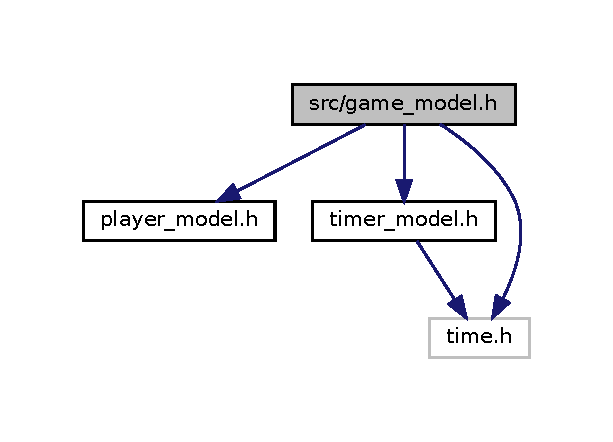
\includegraphics[width=294pt]{game__model_8h__incl}
\end{center}
\end{figure}
Граф файлов, в которые включается этот файл\+:\nopagebreak
\begin{figure}[H]
\begin{center}
\leavevmode
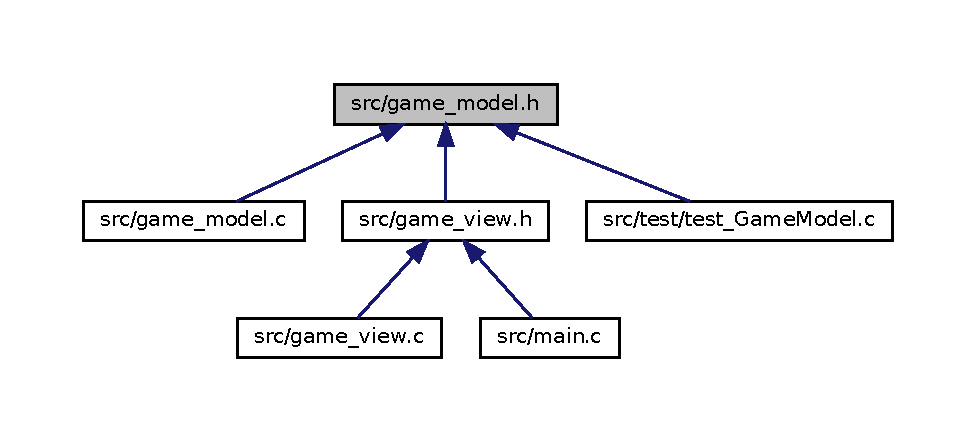
\includegraphics[width=350pt]{game__model_8h__dep__incl}
\end{center}
\end{figure}
\subsection*{Структуры данных}
\begin{DoxyCompactItemize}
\item 
struct \hyperlink{structgame__model}{game\+\_\+model}
\begin{DoxyCompactList}\small\item\em Структура, которая описывает модель игры. \end{DoxyCompactList}\end{DoxyCompactItemize}
\subsection*{Макросы}
\begin{DoxyCompactItemize}
\item 
\#define \hyperlink{game__model_8h_a04a62ceefc64de6e9f0b23e5ef8679cf}{N\+U\+M\+\_\+\+P\+U\+S\+H\+\_\+\+S\+I\+ZE}~(\hyperlink{timer__model_8h_a5ff1ef7bd6c1df2a650162766a2ddb76}{M\+A\+X\+\_\+\+MN} $\ast$ \hyperlink{timer__model_8h_ab96c94c7d4f72592fb0bd579675c89f2}{M\+A\+X\+\_\+\+S\+EC})
\begin{DoxyCompactList}\small\item\em Максимальная продолжительность игры в секундах. \end{DoxyCompactList}\item 
\#define \hyperlink{game__model_8h_aa6bd5b4fb706f2be4aa638b486e8b103}{S\+P\+E\+E\+D\+\_\+\+D\+O\+W\+N\+\_\+\+F\+A\+C\+T\+OR}~3
\begin{DoxyCompactList}\small\item\em Коэффициент расчета скорости №1. \end{DoxyCompactList}\item 
\#define \hyperlink{game__model_8h_a8dcfb0aedf29314da0c1f2d42f6e0856}{S\+P\+E\+E\+D\+\_\+\+D\+I\+V\+\_\+\+F\+A\+C\+T\+OR}~20
\begin{DoxyCompactList}\small\item\em Коэффициент расчета скорости №2. \end{DoxyCompactList}\end{DoxyCompactItemize}
\subsection*{Определения типов}
\begin{DoxyCompactItemize}
\item 
typedef enum \hyperlink{game__model_8h_ab56b05c2bb34d1168dc2576c83a1e287}{key\+\_\+type} \hyperlink{game__model_8h_aa59688e58fb86c8f53b8ff8cc992507f}{key\+\_\+type}
\item 
typedef struct \hyperlink{structgame__model}{game\+\_\+model} \hyperlink{game__model_8h_a5e0a3ee36570d19d482a26dcc6c9b0fb}{game\+\_\+model}
\end{DoxyCompactItemize}
\subsection*{Перечисления}
\begin{DoxyCompactItemize}
\item 
enum \hyperlink{game__model_8h_ab56b05c2bb34d1168dc2576c83a1e287}{key\+\_\+type} \{ \hyperlink{game__model_8h_ab56b05c2bb34d1168dc2576c83a1e287adb45120aafd37a973140edee24708065}{L\+E\+FT}, 
\hyperlink{game__model_8h_ab56b05c2bb34d1168dc2576c83a1e287aec8379af7490bb9eaaf579cf17876f38}{R\+I\+G\+HT}, 
\hyperlink{game__model_8h_ab56b05c2bb34d1168dc2576c83a1e287adbf1dee1b8cd7ea3c82661943c7b74f4}{O\+T\+H\+ER}
 \}\begin{DoxyCompactList}\small\item\em Тип нажимаемой клавиши. \end{DoxyCompactList}
\end{DoxyCompactItemize}
\subsection*{Функции}
\begin{DoxyCompactItemize}
\item 
\hyperlink{structgame__model}{game\+\_\+model} $\ast$ \hyperlink{game__model_8h_aaad3a76b7ba25cb7490c5830baa7432a}{game\+\_\+model\+\_\+create} ()
\item 
int \hyperlink{game__model_8h_a79ebd68f67408541b9783c84c3bbc0cd}{game\+\_\+model\+\_\+key\+\_\+down} (\hyperlink{structgame__model}{game\+\_\+model} $\ast$g\+\_\+model, \hyperlink{game__model_8h_ab56b05c2bb34d1168dc2576c83a1e287}{key\+\_\+type} k\+\_\+type)
\item 
int \hyperlink{game__model_8h_a7b376d7df735e44499029175f25d7dc2}{game\+\_\+model\+\_\+update} (\hyperlink{structgame__model}{game\+\_\+model} $\ast$g\+\_\+model)
\item 
int \hyperlink{game__model_8h_a664d5848306405c334826f6dd5a6de21}{game\+\_\+model\+\_\+start} (\hyperlink{structgame__model}{game\+\_\+model} $\ast$g\+\_\+model)
\item 
int \hyperlink{game__model_8h_a9b1e18809a52c5132f77e53fdae2edd6}{game\+\_\+model\+\_\+is\+\_\+end} (\hyperlink{structgame__model}{game\+\_\+model} $\ast$g\+\_\+model)
\item 
int \hyperlink{game__model_8h_ac392382451e375796a63240a776c270f}{game\+\_\+model\+\_\+destroy} (\hyperlink{structgame__model}{game\+\_\+model} $\ast$g\+\_\+model)
\end{DoxyCompactItemize}


\subsection{Подробное описание}
Файл, в котором опеределены функции для работы с моделью игры. 



\subsection{Макросы}
\mbox{\Hypertarget{game__model_8h_a04a62ceefc64de6e9f0b23e5ef8679cf}\label{game__model_8h_a04a62ceefc64de6e9f0b23e5ef8679cf}} 
\index{game\+\_\+model.\+h@{game\+\_\+model.\+h}!N\+U\+M\+\_\+\+P\+U\+S\+H\+\_\+\+S\+I\+ZE@{N\+U\+M\+\_\+\+P\+U\+S\+H\+\_\+\+S\+I\+ZE}}
\index{N\+U\+M\+\_\+\+P\+U\+S\+H\+\_\+\+S\+I\+ZE@{N\+U\+M\+\_\+\+P\+U\+S\+H\+\_\+\+S\+I\+ZE}!game\+\_\+model.\+h@{game\+\_\+model.\+h}}
\subsubsection{\texorpdfstring{N\+U\+M\+\_\+\+P\+U\+S\+H\+\_\+\+S\+I\+ZE}{NUM\_PUSH\_SIZE}}
{\footnotesize\ttfamily \#define N\+U\+M\+\_\+\+P\+U\+S\+H\+\_\+\+S\+I\+ZE~(\hyperlink{timer__model_8h_a5ff1ef7bd6c1df2a650162766a2ddb76}{M\+A\+X\+\_\+\+MN} $\ast$ \hyperlink{timer__model_8h_ab96c94c7d4f72592fb0bd579675c89f2}{M\+A\+X\+\_\+\+S\+EC})}



Максимальная продолжительность игры в секундах. 

\mbox{\Hypertarget{game__model_8h_a8dcfb0aedf29314da0c1f2d42f6e0856}\label{game__model_8h_a8dcfb0aedf29314da0c1f2d42f6e0856}} 
\index{game\+\_\+model.\+h@{game\+\_\+model.\+h}!S\+P\+E\+E\+D\+\_\+\+D\+I\+V\+\_\+\+F\+A\+C\+T\+OR@{S\+P\+E\+E\+D\+\_\+\+D\+I\+V\+\_\+\+F\+A\+C\+T\+OR}}
\index{S\+P\+E\+E\+D\+\_\+\+D\+I\+V\+\_\+\+F\+A\+C\+T\+OR@{S\+P\+E\+E\+D\+\_\+\+D\+I\+V\+\_\+\+F\+A\+C\+T\+OR}!game\+\_\+model.\+h@{game\+\_\+model.\+h}}
\subsubsection{\texorpdfstring{S\+P\+E\+E\+D\+\_\+\+D\+I\+V\+\_\+\+F\+A\+C\+T\+OR}{SPEED\_DIV\_FACTOR}}
{\footnotesize\ttfamily \#define S\+P\+E\+E\+D\+\_\+\+D\+I\+V\+\_\+\+F\+A\+C\+T\+OR~20}



Коэффициент расчета скорости №2. 

\mbox{\Hypertarget{game__model_8h_aa6bd5b4fb706f2be4aa638b486e8b103}\label{game__model_8h_aa6bd5b4fb706f2be4aa638b486e8b103}} 
\index{game\+\_\+model.\+h@{game\+\_\+model.\+h}!S\+P\+E\+E\+D\+\_\+\+D\+O\+W\+N\+\_\+\+F\+A\+C\+T\+OR@{S\+P\+E\+E\+D\+\_\+\+D\+O\+W\+N\+\_\+\+F\+A\+C\+T\+OR}}
\index{S\+P\+E\+E\+D\+\_\+\+D\+O\+W\+N\+\_\+\+F\+A\+C\+T\+OR@{S\+P\+E\+E\+D\+\_\+\+D\+O\+W\+N\+\_\+\+F\+A\+C\+T\+OR}!game\+\_\+model.\+h@{game\+\_\+model.\+h}}
\subsubsection{\texorpdfstring{S\+P\+E\+E\+D\+\_\+\+D\+O\+W\+N\+\_\+\+F\+A\+C\+T\+OR}{SPEED\_DOWN\_FACTOR}}
{\footnotesize\ttfamily \#define S\+P\+E\+E\+D\+\_\+\+D\+O\+W\+N\+\_\+\+F\+A\+C\+T\+OR~3}



Коэффициент расчета скорости №1. 



\subsection{Типы}
\mbox{\Hypertarget{game__model_8h_a5e0a3ee36570d19d482a26dcc6c9b0fb}\label{game__model_8h_a5e0a3ee36570d19d482a26dcc6c9b0fb}} 
\index{game\+\_\+model.\+h@{game\+\_\+model.\+h}!game\+\_\+model@{game\+\_\+model}}
\index{game\+\_\+model@{game\+\_\+model}!game\+\_\+model.\+h@{game\+\_\+model.\+h}}
\subsubsection{\texorpdfstring{game\+\_\+model}{game\_model}}
{\footnotesize\ttfamily typedef struct \hyperlink{structgame__model}{game\+\_\+model} \hyperlink{structgame__model}{game\+\_\+model}}

\mbox{\Hypertarget{game__model_8h_aa59688e58fb86c8f53b8ff8cc992507f}\label{game__model_8h_aa59688e58fb86c8f53b8ff8cc992507f}} 
\index{game\+\_\+model.\+h@{game\+\_\+model.\+h}!key\+\_\+type@{key\+\_\+type}}
\index{key\+\_\+type@{key\+\_\+type}!game\+\_\+model.\+h@{game\+\_\+model.\+h}}
\subsubsection{\texorpdfstring{key\+\_\+type}{key\_type}}
{\footnotesize\ttfamily typedef enum \hyperlink{game__model_8h_ab56b05c2bb34d1168dc2576c83a1e287}{key\+\_\+type} \hyperlink{game__model_8h_ab56b05c2bb34d1168dc2576c83a1e287}{key\+\_\+type}}



\subsection{Перечисления}
\mbox{\Hypertarget{game__model_8h_ab56b05c2bb34d1168dc2576c83a1e287}\label{game__model_8h_ab56b05c2bb34d1168dc2576c83a1e287}} 
\index{game\+\_\+model.\+h@{game\+\_\+model.\+h}!key\+\_\+type@{key\+\_\+type}}
\index{key\+\_\+type@{key\+\_\+type}!game\+\_\+model.\+h@{game\+\_\+model.\+h}}
\subsubsection{\texorpdfstring{key\+\_\+type}{key\_type}}
{\footnotesize\ttfamily enum \hyperlink{game__model_8h_ab56b05c2bb34d1168dc2576c83a1e287}{key\+\_\+type}}



Тип нажимаемой клавиши. 

\begin{DoxyEnumFields}{Элементы перечислений}
\raisebox{\heightof{T}}[0pt][0pt]{\index{L\+E\+FT@{L\+E\+FT}!game\+\_\+model.\+h@{game\+\_\+model.\+h}}\index{game\+\_\+model.\+h@{game\+\_\+model.\+h}!L\+E\+FT@{L\+E\+FT}}}\mbox{\Hypertarget{game__model_8h_ab56b05c2bb34d1168dc2576c83a1e287adb45120aafd37a973140edee24708065}\label{game__model_8h_ab56b05c2bb34d1168dc2576c83a1e287adb45120aafd37a973140edee24708065}} 
L\+E\+FT&Стрелка влево. \\
\hline

\raisebox{\heightof{T}}[0pt][0pt]{\index{R\+I\+G\+HT@{R\+I\+G\+HT}!game\+\_\+model.\+h@{game\+\_\+model.\+h}}\index{game\+\_\+model.\+h@{game\+\_\+model.\+h}!R\+I\+G\+HT@{R\+I\+G\+HT}}}\mbox{\Hypertarget{game__model_8h_ab56b05c2bb34d1168dc2576c83a1e287aec8379af7490bb9eaaf579cf17876f38}\label{game__model_8h_ab56b05c2bb34d1168dc2576c83a1e287aec8379af7490bb9eaaf579cf17876f38}} 
R\+I\+G\+HT&Стрелка вправо. \\
\hline

\raisebox{\heightof{T}}[0pt][0pt]{\index{O\+T\+H\+ER@{O\+T\+H\+ER}!game\+\_\+model.\+h@{game\+\_\+model.\+h}}\index{game\+\_\+model.\+h@{game\+\_\+model.\+h}!O\+T\+H\+ER@{O\+T\+H\+ER}}}\mbox{\Hypertarget{game__model_8h_ab56b05c2bb34d1168dc2576c83a1e287adbf1dee1b8cd7ea3c82661943c7b74f4}\label{game__model_8h_ab56b05c2bb34d1168dc2576c83a1e287adbf1dee1b8cd7ea3c82661943c7b74f4}} 
O\+T\+H\+ER&Другая клавиша. \\
\hline

\end{DoxyEnumFields}


\subsection{Функции}
\mbox{\Hypertarget{game__model_8h_aaad3a76b7ba25cb7490c5830baa7432a}\label{game__model_8h_aaad3a76b7ba25cb7490c5830baa7432a}} 
\index{game\+\_\+model.\+h@{game\+\_\+model.\+h}!game\+\_\+model\+\_\+create@{game\+\_\+model\+\_\+create}}
\index{game\+\_\+model\+\_\+create@{game\+\_\+model\+\_\+create}!game\+\_\+model.\+h@{game\+\_\+model.\+h}}
\subsubsection{\texorpdfstring{game\+\_\+model\+\_\+create()}{game\_model\_create()}}
{\footnotesize\ttfamily \hyperlink{structgame__model}{game\+\_\+model}$\ast$ game\+\_\+model\+\_\+create (\begin{DoxyParamCaption}{ }\end{DoxyParamCaption})}

Создание модели игры. \begin{DoxyReturn}{Возвращает}
Адрес, созданной модели. ~\newline
 N\+U\+LL, если во время создания модели произошла ошибка. 
\end{DoxyReturn}
\mbox{\Hypertarget{game__model_8h_ac392382451e375796a63240a776c270f}\label{game__model_8h_ac392382451e375796a63240a776c270f}} 
\index{game\+\_\+model.\+h@{game\+\_\+model.\+h}!game\+\_\+model\+\_\+destroy@{game\+\_\+model\+\_\+destroy}}
\index{game\+\_\+model\+\_\+destroy@{game\+\_\+model\+\_\+destroy}!game\+\_\+model.\+h@{game\+\_\+model.\+h}}
\subsubsection{\texorpdfstring{game\+\_\+model\+\_\+destroy()}{game\_model\_destroy()}}
{\footnotesize\ttfamily int game\+\_\+model\+\_\+destroy (\begin{DoxyParamCaption}\item[{\hyperlink{structgame__model}{game\+\_\+model} $\ast$}]{g\+\_\+model }\end{DoxyParamCaption})}

Удаление модели игры. 
\begin{DoxyParams}[1]{Аргументы}
\mbox{\tt in}  & {\em g\+\_\+model} & -\/ адрес модели игры, которую нужно удалить. \\
\hline
\end{DoxyParams}
\begin{DoxyReturn}{Возвращает}
Ноль, если удаление прошло успешно. ~\newline
 Ненулевое число, если во время удаления произошла ошибка. 
\end{DoxyReturn}
\mbox{\Hypertarget{game__model_8h_a9b1e18809a52c5132f77e53fdae2edd6}\label{game__model_8h_a9b1e18809a52c5132f77e53fdae2edd6}} 
\index{game\+\_\+model.\+h@{game\+\_\+model.\+h}!game\+\_\+model\+\_\+is\+\_\+end@{game\+\_\+model\+\_\+is\+\_\+end}}
\index{game\+\_\+model\+\_\+is\+\_\+end@{game\+\_\+model\+\_\+is\+\_\+end}!game\+\_\+model.\+h@{game\+\_\+model.\+h}}
\subsubsection{\texorpdfstring{game\+\_\+model\+\_\+is\+\_\+end()}{game\_model\_is\_end()}}
{\footnotesize\ttfamily int game\+\_\+model\+\_\+is\+\_\+end (\begin{DoxyParamCaption}\item[{\hyperlink{structgame__model}{game\+\_\+model} $\ast$}]{g\+\_\+model }\end{DoxyParamCaption})}

Проверка окончания игры. 
\begin{DoxyParams}[1]{Аргументы}
\mbox{\tt in}  & {\em g\+\_\+model} & -\/ адрес модели игры, которую нужно проверить. \\
\hline
\end{DoxyParams}
\begin{DoxyReturn}{Возвращает}
Отрицательное число, если во время проверки произошла ошибка. ~\newline
 Ноль, если игра еще не закончилась. ~\newline
 Положительное число, если игра закончилась. 
\end{DoxyReturn}
\mbox{\Hypertarget{game__model_8h_a79ebd68f67408541b9783c84c3bbc0cd}\label{game__model_8h_a79ebd68f67408541b9783c84c3bbc0cd}} 
\index{game\+\_\+model.\+h@{game\+\_\+model.\+h}!game\+\_\+model\+\_\+key\+\_\+down@{game\+\_\+model\+\_\+key\+\_\+down}}
\index{game\+\_\+model\+\_\+key\+\_\+down@{game\+\_\+model\+\_\+key\+\_\+down}!game\+\_\+model.\+h@{game\+\_\+model.\+h}}
\subsubsection{\texorpdfstring{game\+\_\+model\+\_\+key\+\_\+down()}{game\_model\_key\_down()}}
{\footnotesize\ttfamily int game\+\_\+model\+\_\+key\+\_\+down (\begin{DoxyParamCaption}\item[{\hyperlink{structgame__model}{game\+\_\+model} $\ast$}]{g\+\_\+model,  }\item[{\hyperlink{game__model_8h_ab56b05c2bb34d1168dc2576c83a1e287}{key\+\_\+type}}]{k\+\_\+type }\end{DoxyParamCaption})}

Обработка нажатия клавиши. 
\begin{DoxyParams}[1]{Аргументы}
\mbox{\tt in,out}  & {\em g\+\_\+model} & -\/ адрес модели, для которой обрабатывает нажатие. \\
\hline
\mbox{\tt in}  & {\em k\+\_\+type} & -\/ тип нажатой клавиши. \\
\hline
\end{DoxyParams}
\begin{DoxyReturn}{Возвращает}
Ноль, если обработка прошла успешно. ~\newline
 Ненулевое число, если во время обработки произошла ошибка. 
\end{DoxyReturn}
\mbox{\Hypertarget{game__model_8h_a664d5848306405c334826f6dd5a6de21}\label{game__model_8h_a664d5848306405c334826f6dd5a6de21}} 
\index{game\+\_\+model.\+h@{game\+\_\+model.\+h}!game\+\_\+model\+\_\+start@{game\+\_\+model\+\_\+start}}
\index{game\+\_\+model\+\_\+start@{game\+\_\+model\+\_\+start}!game\+\_\+model.\+h@{game\+\_\+model.\+h}}
\subsubsection{\texorpdfstring{game\+\_\+model\+\_\+start()}{game\_model\_start()}}
{\footnotesize\ttfamily int game\+\_\+model\+\_\+start (\begin{DoxyParamCaption}\item[{\hyperlink{structgame__model}{game\+\_\+model} $\ast$}]{g\+\_\+model }\end{DoxyParamCaption})}

Старт игры. 
\begin{DoxyParams}[1]{Аргументы}
\mbox{\tt in,out}  & {\em g\+\_\+model} & -\/ адрес модели игры, которую нужно запустить. \\
\hline
\end{DoxyParams}
\begin{DoxyReturn}{Возвращает}
Ноль, если запуск прошёл успешно. ~\newline
 Ненулевое число, если во время запуска произошла ошибка. 
\end{DoxyReturn}
\mbox{\Hypertarget{game__model_8h_a7b376d7df735e44499029175f25d7dc2}\label{game__model_8h_a7b376d7df735e44499029175f25d7dc2}} 
\index{game\+\_\+model.\+h@{game\+\_\+model.\+h}!game\+\_\+model\+\_\+update@{game\+\_\+model\+\_\+update}}
\index{game\+\_\+model\+\_\+update@{game\+\_\+model\+\_\+update}!game\+\_\+model.\+h@{game\+\_\+model.\+h}}
\subsubsection{\texorpdfstring{game\+\_\+model\+\_\+update()}{game\_model\_update()}}
{\footnotesize\ttfamily int game\+\_\+model\+\_\+update (\begin{DoxyParamCaption}\item[{\hyperlink{structgame__model}{game\+\_\+model} $\ast$}]{g\+\_\+model }\end{DoxyParamCaption})}

Обновление данных модели игры 
\begin{DoxyParams}[1]{Аргументы}
\mbox{\tt in,out}  & {\em g\+\_\+model} & -\/ адрес модели игры, которую необходимо обновить. \\
\hline
\end{DoxyParams}
\begin{DoxyReturn}{Возвращает}
Ноль, если обновление прошло успешно. ~\newline
 Ненулевое число, если во время обновления произошла ошибка. 
\end{DoxyReturn}

\hypertarget{game__view_8c}{}\section{Файл src/game\+\_\+view.c}
\label{game__view_8c}\index{src/game\+\_\+view.\+c@{src/game\+\_\+view.\+c}}


Файл, в котором опеределены функции для работы с отображением игры.  


{\ttfamily \#include \char`\"{}game\+\_\+view.\+h\char`\"{}}\newline
{\ttfamily \#include \char`\"{}error\+\_\+report.\+h\char`\"{}}\newline
{\ttfamily \#include $<$stdlib.\+h$>$}\newline
{\ttfamily \#include $<$stdbool.\+h$>$}\newline
Граф включаемых заголовочных файлов для game\+\_\+view.\+c\+:\nopagebreak
\begin{figure}[H]
\begin{center}
\leavevmode
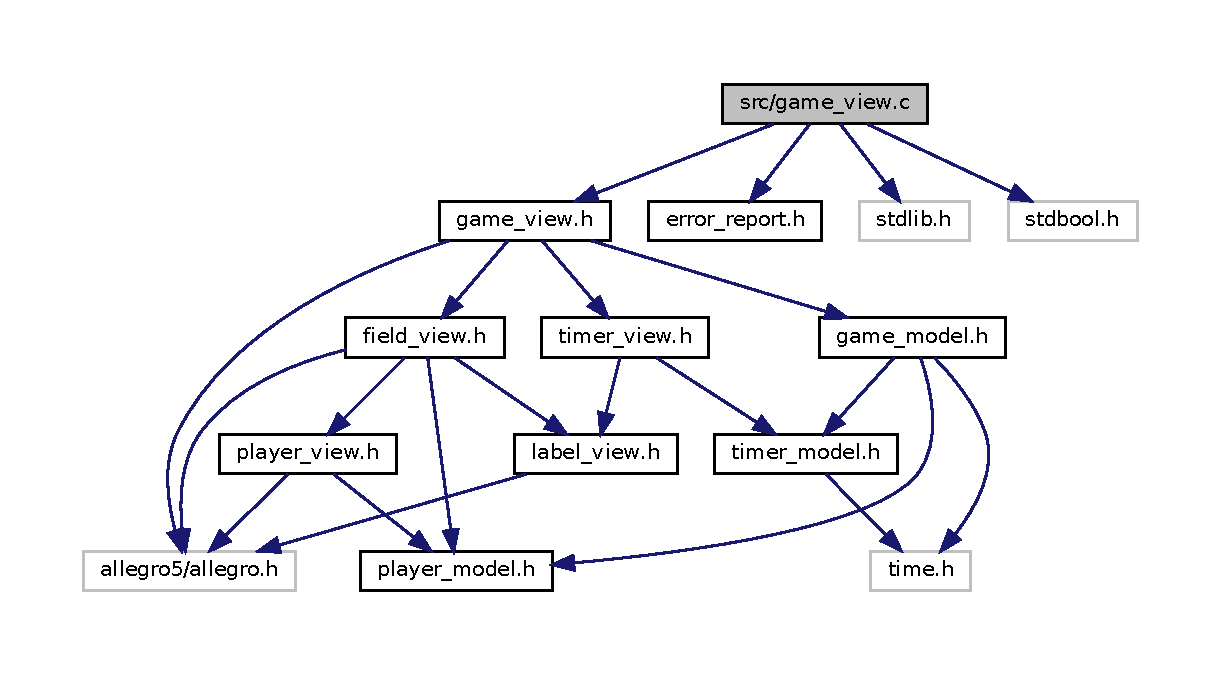
\includegraphics[width=350pt]{game__view_8c__incl}
\end{center}
\end{figure}
\subsection*{Макросы}
\begin{DoxyCompactItemize}
\item 
\#define \hyperlink{game__view_8c_ab117546549783a058d0321a287699579}{F\+I\+L\+E\+\_\+\+N\+A\+ME}~\char`\"{}game\+\_\+view.\+c\char`\"{}
\begin{DoxyCompactList}\small\item\em Имя текущего файла. \end{DoxyCompactList}\item 
\#define \hyperlink{game__view_8c_aba64ab31ac50908f7aa4125955fcf2ed}{F\+U\+N\+\_\+\+N\+A\+ME}~\char`\"{}init\+\_\+allegro\+\_\+field\char`\"{}
\begin{DoxyCompactList}\small\item\em Имя текущей функции. \end{DoxyCompactList}\item 
\#define \hyperlink{game__view_8c_aba64ab31ac50908f7aa4125955fcf2ed}{F\+U\+N\+\_\+\+N\+A\+ME}~\char`\"{}init\+\_\+view\+\_\+and\+\_\+model\+\_\+field\char`\"{}
\begin{DoxyCompactList}\small\item\em Имя текущей функции. \end{DoxyCompactList}\item 
\#define \hyperlink{game__view_8c_aba64ab31ac50908f7aa4125955fcf2ed}{F\+U\+N\+\_\+\+N\+A\+ME}~\char`\"{}game\+\_\+view\+\_\+create\char`\"{}
\begin{DoxyCompactList}\small\item\em Имя текущей функции. \end{DoxyCompactList}\end{DoxyCompactItemize}
\subsection*{Функции}
\begin{DoxyCompactItemize}
\item 
\hyperlink{structgame__view}{game\+\_\+view} $\ast$ \hyperlink{game__view_8c_a5d31da96dc1fcded5af87b110ea1cd98}{game\+\_\+view\+\_\+create} ()
\item 
int \hyperlink{game__view_8c_a58c54dcc496dca3fe69803f83b89a877}{game\+\_\+view\+\_\+start} (\hyperlink{structgame__view}{game\+\_\+view} $\ast$g\+\_\+view)
\item 
int \hyperlink{game__view_8c_abc345bb97069dd789b670fe8f1f23a4d}{game\+\_\+view\+\_\+destroy} (\hyperlink{structgame__view}{game\+\_\+view} $\ast$g\+\_\+view)
\end{DoxyCompactItemize}


\subsection{Подробное описание}
Файл, в котором опеределены функции для работы с отображением игры. 



\subsection{Макросы}
\mbox{\Hypertarget{game__view_8c_ab117546549783a058d0321a287699579}\label{game__view_8c_ab117546549783a058d0321a287699579}} 
\index{game\+\_\+view.\+c@{game\+\_\+view.\+c}!F\+I\+L\+E\+\_\+\+N\+A\+ME@{F\+I\+L\+E\+\_\+\+N\+A\+ME}}
\index{F\+I\+L\+E\+\_\+\+N\+A\+ME@{F\+I\+L\+E\+\_\+\+N\+A\+ME}!game\+\_\+view.\+c@{game\+\_\+view.\+c}}
\subsubsection{\texorpdfstring{F\+I\+L\+E\+\_\+\+N\+A\+ME}{FILE\_NAME}}
{\footnotesize\ttfamily \#define F\+I\+L\+E\+\_\+\+N\+A\+ME~\char`\"{}game\+\_\+view.\+c\char`\"{}}



Имя текущего файла. 

\mbox{\Hypertarget{game__view_8c_aba64ab31ac50908f7aa4125955fcf2ed}\label{game__view_8c_aba64ab31ac50908f7aa4125955fcf2ed}} 
\index{game\+\_\+view.\+c@{game\+\_\+view.\+c}!F\+U\+N\+\_\+\+N\+A\+ME@{F\+U\+N\+\_\+\+N\+A\+ME}}
\index{F\+U\+N\+\_\+\+N\+A\+ME@{F\+U\+N\+\_\+\+N\+A\+ME}!game\+\_\+view.\+c@{game\+\_\+view.\+c}}
\subsubsection{\texorpdfstring{F\+U\+N\+\_\+\+N\+A\+ME}{FUN\_NAME}\hspace{0.1cm}{\footnotesize\ttfamily [1/3]}}
{\footnotesize\ttfamily \#define F\+U\+N\+\_\+\+N\+A\+ME~\char`\"{}init\+\_\+allegro\+\_\+field\char`\"{}}



Имя текущей функции. 

\mbox{\Hypertarget{game__view_8c_aba64ab31ac50908f7aa4125955fcf2ed}\label{game__view_8c_aba64ab31ac50908f7aa4125955fcf2ed}} 
\index{game\+\_\+view.\+c@{game\+\_\+view.\+c}!F\+U\+N\+\_\+\+N\+A\+ME@{F\+U\+N\+\_\+\+N\+A\+ME}}
\index{F\+U\+N\+\_\+\+N\+A\+ME@{F\+U\+N\+\_\+\+N\+A\+ME}!game\+\_\+view.\+c@{game\+\_\+view.\+c}}
\subsubsection{\texorpdfstring{F\+U\+N\+\_\+\+N\+A\+ME}{FUN\_NAME}\hspace{0.1cm}{\footnotesize\ttfamily [2/3]}}
{\footnotesize\ttfamily \#define F\+U\+N\+\_\+\+N\+A\+ME~\char`\"{}init\+\_\+view\+\_\+and\+\_\+model\+\_\+field\char`\"{}}



Имя текущей функции. 

\mbox{\Hypertarget{game__view_8c_aba64ab31ac50908f7aa4125955fcf2ed}\label{game__view_8c_aba64ab31ac50908f7aa4125955fcf2ed}} 
\index{game\+\_\+view.\+c@{game\+\_\+view.\+c}!F\+U\+N\+\_\+\+N\+A\+ME@{F\+U\+N\+\_\+\+N\+A\+ME}}
\index{F\+U\+N\+\_\+\+N\+A\+ME@{F\+U\+N\+\_\+\+N\+A\+ME}!game\+\_\+view.\+c@{game\+\_\+view.\+c}}
\subsubsection{\texorpdfstring{F\+U\+N\+\_\+\+N\+A\+ME}{FUN\_NAME}\hspace{0.1cm}{\footnotesize\ttfamily [3/3]}}
{\footnotesize\ttfamily \#define F\+U\+N\+\_\+\+N\+A\+ME~\char`\"{}game\+\_\+view\+\_\+create\char`\"{}}



Имя текущей функции. 



\subsection{Функции}
\mbox{\Hypertarget{game__view_8c_a5d31da96dc1fcded5af87b110ea1cd98}\label{game__view_8c_a5d31da96dc1fcded5af87b110ea1cd98}} 
\index{game\+\_\+view.\+c@{game\+\_\+view.\+c}!game\+\_\+view\+\_\+create@{game\+\_\+view\+\_\+create}}
\index{game\+\_\+view\+\_\+create@{game\+\_\+view\+\_\+create}!game\+\_\+view.\+c@{game\+\_\+view.\+c}}
\subsubsection{\texorpdfstring{game\+\_\+view\+\_\+create()}{game\_view\_create()}}
{\footnotesize\ttfamily \hyperlink{structgame__view}{game\+\_\+view}$\ast$ game\+\_\+view\+\_\+create (\begin{DoxyParamCaption}{ }\end{DoxyParamCaption})}

Создание отображения игры. \begin{DoxyReturn}{Возвращает}
Адрес, созданного отображения игры. ~\newline
 N\+U\+LL, если во время создания отображения игры произошла ошибка. 
\end{DoxyReturn}
\mbox{\Hypertarget{game__view_8c_abc345bb97069dd789b670fe8f1f23a4d}\label{game__view_8c_abc345bb97069dd789b670fe8f1f23a4d}} 
\index{game\+\_\+view.\+c@{game\+\_\+view.\+c}!game\+\_\+view\+\_\+destroy@{game\+\_\+view\+\_\+destroy}}
\index{game\+\_\+view\+\_\+destroy@{game\+\_\+view\+\_\+destroy}!game\+\_\+view.\+c@{game\+\_\+view.\+c}}
\subsubsection{\texorpdfstring{game\+\_\+view\+\_\+destroy()}{game\_view\_destroy()}}
{\footnotesize\ttfamily int game\+\_\+view\+\_\+destroy (\begin{DoxyParamCaption}\item[{\hyperlink{structgame__view}{game\+\_\+view} $\ast$}]{g\+\_\+view }\end{DoxyParamCaption})}

Удаление отображения игры. 
\begin{DoxyParams}[1]{Аргументы}
\mbox{\tt in}  & {\em g\+\_\+view} & -\/ адрес отображения игры, которое нужно удалить. \\
\hline
\end{DoxyParams}
\begin{DoxyReturn}{Возвращает}
Ноль, если удаление прошло успешно. ~\newline
 Ненулевое число, если во время удаления произошла ошибка. 
\end{DoxyReturn}
\mbox{\Hypertarget{game__view_8c_a58c54dcc496dca3fe69803f83b89a877}\label{game__view_8c_a58c54dcc496dca3fe69803f83b89a877}} 
\index{game\+\_\+view.\+c@{game\+\_\+view.\+c}!game\+\_\+view\+\_\+start@{game\+\_\+view\+\_\+start}}
\index{game\+\_\+view\+\_\+start@{game\+\_\+view\+\_\+start}!game\+\_\+view.\+c@{game\+\_\+view.\+c}}
\subsubsection{\texorpdfstring{game\+\_\+view\+\_\+start()}{game\_view\_start()}}
{\footnotesize\ttfamily int game\+\_\+view\+\_\+start (\begin{DoxyParamCaption}\item[{\hyperlink{structgame__view}{game\+\_\+view} $\ast$}]{g\+\_\+view }\end{DoxyParamCaption})}

Старт игры. 
\begin{DoxyParams}[1]{Аргументы}
\mbox{\tt in,out}  & {\em g\+\_\+view} & -\/ адрес отображения игры, которую нужно начать. \\
\hline
\end{DoxyParams}
\begin{DoxyReturn}{Возвращает}
Ноль, если игра успешно закончилась. ~\newline
 Ненулево число, если игра было преджевременно прекращена. 
\end{DoxyReturn}

\hypertarget{game__view_8h}{}\section{Файл src/game\+\_\+view.h}
\label{game__view_8h}\index{src/game\+\_\+view.\+h@{src/game\+\_\+view.\+h}}


Файл, в котором опеределены функции для работы с отображением игры.  


{\ttfamily \#include \char`\"{}game\+\_\+model.\+h\char`\"{}}\newline
{\ttfamily \#include \char`\"{}field\+\_\+view.\+h\char`\"{}}\newline
{\ttfamily \#include \char`\"{}timer\+\_\+view.\+h\char`\"{}}\newline
{\ttfamily \#include $<$allegro5/allegro.\+h$>$}\newline
Граф включаемых заголовочных файлов для game\+\_\+view.\+h\+:\nopagebreak
\begin{figure}[H]
\begin{center}
\leavevmode
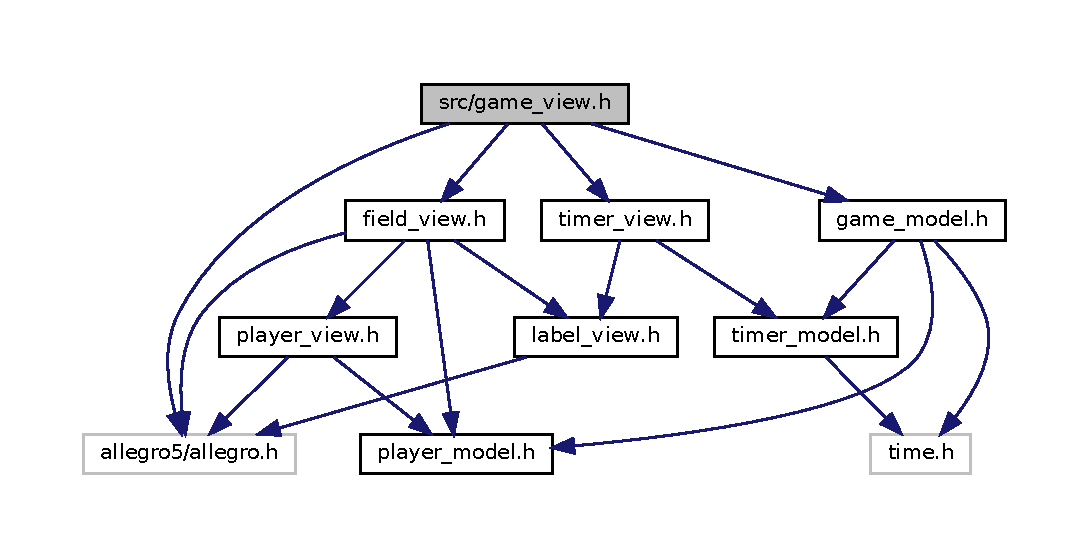
\includegraphics[width=350pt]{game__view_8h__incl}
\end{center}
\end{figure}
Граф файлов, в которые включается этот файл\+:\nopagebreak
\begin{figure}[H]
\begin{center}
\leavevmode
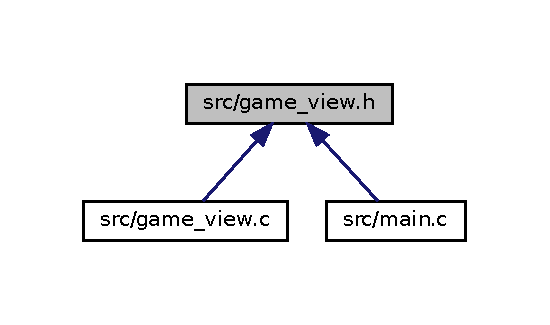
\includegraphics[width=264pt]{game__view_8h__dep__incl}
\end{center}
\end{figure}
\subsection*{Структуры данных}
\begin{DoxyCompactItemize}
\item 
struct \hyperlink{structgame__view}{game\+\_\+view}
\begin{DoxyCompactList}\small\item\em Структура, которая описывает отображение игры. \end{DoxyCompactList}\end{DoxyCompactItemize}
\subsection*{Макросы}
\begin{DoxyCompactItemize}
\item 
\#define \hyperlink{game__view_8h_ac92ca5ab87034a348decad7ee8d4bd1b}{F\+PS}~60
\begin{DoxyCompactList}\small\item\em Частота обновления кадров в секунду. \end{DoxyCompactList}\item 
\#define \hyperlink{game__view_8h_a2cd109632a6dcccaa80b43561b1ab700}{S\+C\+R\+E\+E\+N\+\_\+\+W\+I\+D\+TH}~800
\begin{DoxyCompactList}\small\item\em Ширина экрана. \end{DoxyCompactList}\item 
\#define \hyperlink{game__view_8h_a6974d08a74da681b3957b2fead2608b8}{S\+C\+R\+E\+E\+N\+\_\+\+H\+E\+I\+G\+HT}~600
\begin{DoxyCompactList}\small\item\em Высота экрана. \end{DoxyCompactList}\item 
\#define \hyperlink{game__view_8h_a1c621d1e6010992bc7f6f9f0472495cc}{G\+A\+M\+E\+\_\+\+V\+\_\+\+B\+A\+C\+K\+G\+R\+O\+U\+ND}~al\+\_\+map\+\_\+rgb(255, 255, 255)
\begin{DoxyCompactList}\small\item\em Цвет фона. \end{DoxyCompactList}\end{DoxyCompactItemize}
\subsection*{Определения типов}
\begin{DoxyCompactItemize}
\item 
typedef struct \hyperlink{structgame__view}{game\+\_\+view} \hyperlink{game__view_8h_a65989b0931b52a73cb13d10fd2ae77dd}{game\+\_\+view}
\end{DoxyCompactItemize}
\subsection*{Функции}
\begin{DoxyCompactItemize}
\item 
\hyperlink{structgame__view}{game\+\_\+view} $\ast$ \hyperlink{game__view_8h_a5d31da96dc1fcded5af87b110ea1cd98}{game\+\_\+view\+\_\+create} ()
\item 
int \hyperlink{game__view_8h_a58c54dcc496dca3fe69803f83b89a877}{game\+\_\+view\+\_\+start} (\hyperlink{structgame__view}{game\+\_\+view} $\ast$g\+\_\+view)
\item 
int \hyperlink{game__view_8h_abc345bb97069dd789b670fe8f1f23a4d}{game\+\_\+view\+\_\+destroy} (\hyperlink{structgame__view}{game\+\_\+view} $\ast$g\+\_\+view)
\end{DoxyCompactItemize}


\subsection{Подробное описание}
Файл, в котором опеределены функции для работы с отображением игры. 



\subsection{Макросы}
\mbox{\Hypertarget{game__view_8h_ac92ca5ab87034a348decad7ee8d4bd1b}\label{game__view_8h_ac92ca5ab87034a348decad7ee8d4bd1b}} 
\index{game\+\_\+view.\+h@{game\+\_\+view.\+h}!F\+PS@{F\+PS}}
\index{F\+PS@{F\+PS}!game\+\_\+view.\+h@{game\+\_\+view.\+h}}
\subsubsection{\texorpdfstring{F\+PS}{FPS}}
{\footnotesize\ttfamily \#define F\+PS~60}



Частота обновления кадров в секунду. 

\mbox{\Hypertarget{game__view_8h_a1c621d1e6010992bc7f6f9f0472495cc}\label{game__view_8h_a1c621d1e6010992bc7f6f9f0472495cc}} 
\index{game\+\_\+view.\+h@{game\+\_\+view.\+h}!G\+A\+M\+E\+\_\+\+V\+\_\+\+B\+A\+C\+K\+G\+R\+O\+U\+ND@{G\+A\+M\+E\+\_\+\+V\+\_\+\+B\+A\+C\+K\+G\+R\+O\+U\+ND}}
\index{G\+A\+M\+E\+\_\+\+V\+\_\+\+B\+A\+C\+K\+G\+R\+O\+U\+ND@{G\+A\+M\+E\+\_\+\+V\+\_\+\+B\+A\+C\+K\+G\+R\+O\+U\+ND}!game\+\_\+view.\+h@{game\+\_\+view.\+h}}
\subsubsection{\texorpdfstring{G\+A\+M\+E\+\_\+\+V\+\_\+\+B\+A\+C\+K\+G\+R\+O\+U\+ND}{GAME\_V\_BACKGROUND}}
{\footnotesize\ttfamily \#define G\+A\+M\+E\+\_\+\+V\+\_\+\+B\+A\+C\+K\+G\+R\+O\+U\+ND~al\+\_\+map\+\_\+rgb(255, 255, 255)}



Цвет фона. 

\mbox{\Hypertarget{game__view_8h_a6974d08a74da681b3957b2fead2608b8}\label{game__view_8h_a6974d08a74da681b3957b2fead2608b8}} 
\index{game\+\_\+view.\+h@{game\+\_\+view.\+h}!S\+C\+R\+E\+E\+N\+\_\+\+H\+E\+I\+G\+HT@{S\+C\+R\+E\+E\+N\+\_\+\+H\+E\+I\+G\+HT}}
\index{S\+C\+R\+E\+E\+N\+\_\+\+H\+E\+I\+G\+HT@{S\+C\+R\+E\+E\+N\+\_\+\+H\+E\+I\+G\+HT}!game\+\_\+view.\+h@{game\+\_\+view.\+h}}
\subsubsection{\texorpdfstring{S\+C\+R\+E\+E\+N\+\_\+\+H\+E\+I\+G\+HT}{SCREEN\_HEIGHT}}
{\footnotesize\ttfamily \#define S\+C\+R\+E\+E\+N\+\_\+\+H\+E\+I\+G\+HT~600}



Высота экрана. 

\mbox{\Hypertarget{game__view_8h_a2cd109632a6dcccaa80b43561b1ab700}\label{game__view_8h_a2cd109632a6dcccaa80b43561b1ab700}} 
\index{game\+\_\+view.\+h@{game\+\_\+view.\+h}!S\+C\+R\+E\+E\+N\+\_\+\+W\+I\+D\+TH@{S\+C\+R\+E\+E\+N\+\_\+\+W\+I\+D\+TH}}
\index{S\+C\+R\+E\+E\+N\+\_\+\+W\+I\+D\+TH@{S\+C\+R\+E\+E\+N\+\_\+\+W\+I\+D\+TH}!game\+\_\+view.\+h@{game\+\_\+view.\+h}}
\subsubsection{\texorpdfstring{S\+C\+R\+E\+E\+N\+\_\+\+W\+I\+D\+TH}{SCREEN\_WIDTH}}
{\footnotesize\ttfamily \#define S\+C\+R\+E\+E\+N\+\_\+\+W\+I\+D\+TH~800}



Ширина экрана. 



\subsection{Типы}
\mbox{\Hypertarget{game__view_8h_a65989b0931b52a73cb13d10fd2ae77dd}\label{game__view_8h_a65989b0931b52a73cb13d10fd2ae77dd}} 
\index{game\+\_\+view.\+h@{game\+\_\+view.\+h}!game\+\_\+view@{game\+\_\+view}}
\index{game\+\_\+view@{game\+\_\+view}!game\+\_\+view.\+h@{game\+\_\+view.\+h}}
\subsubsection{\texorpdfstring{game\+\_\+view}{game\_view}}
{\footnotesize\ttfamily typedef struct \hyperlink{structgame__view}{game\+\_\+view} \hyperlink{structgame__view}{game\+\_\+view}}



\subsection{Функции}
\mbox{\Hypertarget{game__view_8h_a5d31da96dc1fcded5af87b110ea1cd98}\label{game__view_8h_a5d31da96dc1fcded5af87b110ea1cd98}} 
\index{game\+\_\+view.\+h@{game\+\_\+view.\+h}!game\+\_\+view\+\_\+create@{game\+\_\+view\+\_\+create}}
\index{game\+\_\+view\+\_\+create@{game\+\_\+view\+\_\+create}!game\+\_\+view.\+h@{game\+\_\+view.\+h}}
\subsubsection{\texorpdfstring{game\+\_\+view\+\_\+create()}{game\_view\_create()}}
{\footnotesize\ttfamily \hyperlink{structgame__view}{game\+\_\+view}$\ast$ game\+\_\+view\+\_\+create (\begin{DoxyParamCaption}{ }\end{DoxyParamCaption})}

Создание отображения игры. \begin{DoxyReturn}{Возвращает}
Адрес, созданного отображения игры. ~\newline
 N\+U\+LL, если во время создания отображения игры произошла ошибка. 
\end{DoxyReturn}
\mbox{\Hypertarget{game__view_8h_abc345bb97069dd789b670fe8f1f23a4d}\label{game__view_8h_abc345bb97069dd789b670fe8f1f23a4d}} 
\index{game\+\_\+view.\+h@{game\+\_\+view.\+h}!game\+\_\+view\+\_\+destroy@{game\+\_\+view\+\_\+destroy}}
\index{game\+\_\+view\+\_\+destroy@{game\+\_\+view\+\_\+destroy}!game\+\_\+view.\+h@{game\+\_\+view.\+h}}
\subsubsection{\texorpdfstring{game\+\_\+view\+\_\+destroy()}{game\_view\_destroy()}}
{\footnotesize\ttfamily int game\+\_\+view\+\_\+destroy (\begin{DoxyParamCaption}\item[{\hyperlink{structgame__view}{game\+\_\+view} $\ast$}]{g\+\_\+view }\end{DoxyParamCaption})}

Удаление отображения игры. 
\begin{DoxyParams}[1]{Аргументы}
\mbox{\tt in}  & {\em g\+\_\+view} & -\/ адрес отображения игры, которое нужно удалить. \\
\hline
\end{DoxyParams}
\begin{DoxyReturn}{Возвращает}
Ноль, если удаление прошло успешно. ~\newline
 Ненулевое число, если во время удаления произошла ошибка. 
\end{DoxyReturn}
\mbox{\Hypertarget{game__view_8h_a58c54dcc496dca3fe69803f83b89a877}\label{game__view_8h_a58c54dcc496dca3fe69803f83b89a877}} 
\index{game\+\_\+view.\+h@{game\+\_\+view.\+h}!game\+\_\+view\+\_\+start@{game\+\_\+view\+\_\+start}}
\index{game\+\_\+view\+\_\+start@{game\+\_\+view\+\_\+start}!game\+\_\+view.\+h@{game\+\_\+view.\+h}}
\subsubsection{\texorpdfstring{game\+\_\+view\+\_\+start()}{game\_view\_start()}}
{\footnotesize\ttfamily int game\+\_\+view\+\_\+start (\begin{DoxyParamCaption}\item[{\hyperlink{structgame__view}{game\+\_\+view} $\ast$}]{g\+\_\+view }\end{DoxyParamCaption})}

Старт игры. 
\begin{DoxyParams}[1]{Аргументы}
\mbox{\tt in,out}  & {\em g\+\_\+view} & -\/ адрес отображения игры, которую нужно начать. \\
\hline
\end{DoxyParams}
\begin{DoxyReturn}{Возвращает}
Ноль, если игра успешно закончилась. ~\newline
 Ненулево число, если игра было преджевременно прекращена. 
\end{DoxyReturn}

\hypertarget{label__view_8c}{}\section{Файл src/label\+\_\+view.c}
\label{label__view_8c}\index{src/label\+\_\+view.\+c@{src/label\+\_\+view.\+c}}


Файл, в котором реализованы функции для работы с элементом интерфейса\+: \char`\"{}надпись\char`\"{}.  


{\ttfamily \#include \char`\"{}label\+\_\+view.\+h\char`\"{}}\newline
{\ttfamily \#include \char`\"{}rectangle\+\_\+view.\+h\char`\"{}}\newline
{\ttfamily \#include \char`\"{}error\+\_\+report.\+h\char`\"{}}\newline
{\ttfamily \#include $<$stdlib.\+h$>$}\newline
{\ttfamily \#include $<$string.\+h$>$}\newline
{\ttfamily \#include $<$allegro5/allegro\+\_\+font.\+h$>$}\newline
{\ttfamily \#include $<$allegro5/allegro\+\_\+ttf.\+h$>$}\newline
Граф включаемых заголовочных файлов для label\+\_\+view.\+c\+:\nopagebreak
\begin{figure}[H]
\begin{center}
\leavevmode
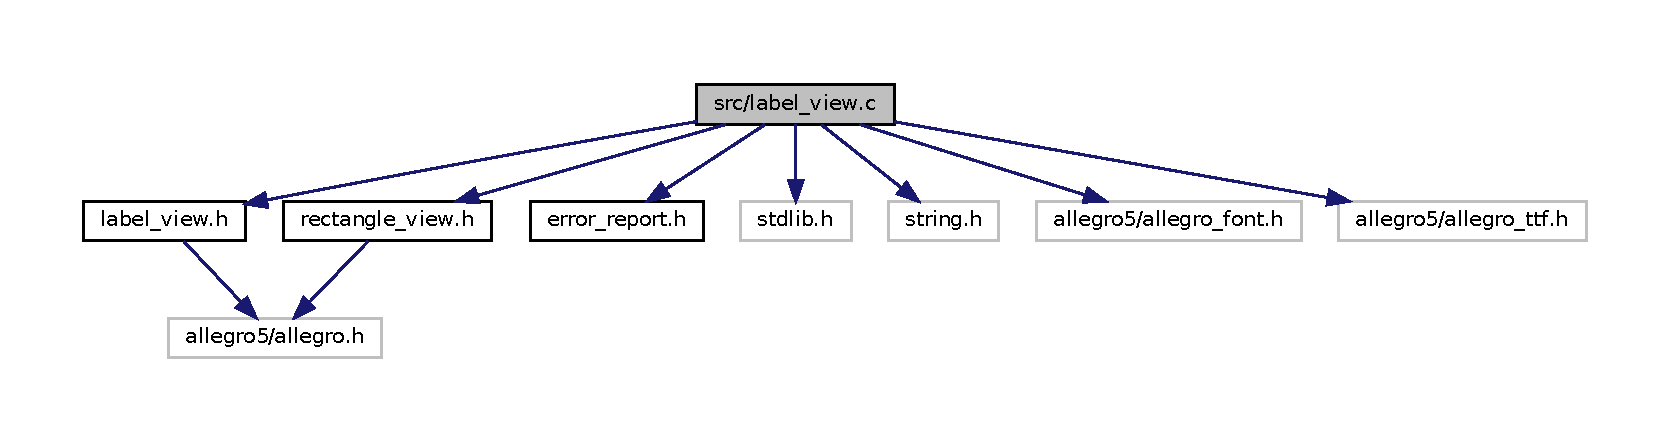
\includegraphics[width=350pt]{label__view_8c__incl}
\end{center}
\end{figure}
\subsection*{Макросы}
\begin{DoxyCompactItemize}
\item 
\#define \hyperlink{label__view_8c_a2c53d2bdf06b28382a374abb3bd92e63}{L\+A\+B\+E\+L\+\_\+\+B\+O\+R\+D\+E\+R\+\_\+\+S\+I\+ZE}~10
\begin{DoxyCompactList}\small\item\em Размер рамки. \end{DoxyCompactList}\item 
\#define \hyperlink{label__view_8c_a1610a21b358c3531db64b3208fa70e5b}{M\+I\+N\+\_\+\+H\+E\+I\+G\+HT}~(\hyperlink{label__view_8c_a2c53d2bdf06b28382a374abb3bd92e63}{L\+A\+B\+E\+L\+\_\+\+B\+O\+R\+D\+E\+R\+\_\+\+S\+I\+ZE} $\ast$ 2 + 10)
\begin{DoxyCompactList}\small\item\em Минимальная высота надписи. \end{DoxyCompactList}\item 
\#define \hyperlink{label__view_8c_ad3ee0cc681d736cb6d41c4ebb04c0ae4}{M\+I\+N\+\_\+\+W\+I\+D\+TH}~(\hyperlink{label__view_8c_a2c53d2bdf06b28382a374abb3bd92e63}{L\+A\+B\+E\+L\+\_\+\+B\+O\+R\+D\+E\+R\+\_\+\+S\+I\+ZE} $\ast$ 2 + 45)
\begin{DoxyCompactList}\small\item\em Минимальная ширина надписи. \end{DoxyCompactList}\item 
\#define \hyperlink{label__view_8c_a806c5e8aebd09085d3d46107c7283e71}{P\+A\+T\+H\+\_\+\+F\+O\+NT}~\char`\"{}res/Very\+Convincing.\+ttf\char`\"{}
\begin{DoxyCompactList}\small\item\em Путь к файлу со шрифтом. \end{DoxyCompactList}\item 
\#define \hyperlink{label__view_8c_ab117546549783a058d0321a287699579}{F\+I\+L\+E\+\_\+\+N\+A\+ME}~\char`\"{}label\+\_\+view.\+c\char`\"{}
\begin{DoxyCompactList}\small\item\em Имя текущего файла. \end{DoxyCompactList}\item 
\#define \hyperlink{label__view_8c_aba64ab31ac50908f7aa4125955fcf2ed}{F\+U\+N\+\_\+\+N\+A\+ME}~\char`\"{}label\+\_\+view\+\_\+init\+\_\+font\char`\"{}
\begin{DoxyCompactList}\small\item\em Имя текущей функции. \end{DoxyCompactList}\item 
\#define \hyperlink{label__view_8c_aba64ab31ac50908f7aa4125955fcf2ed}{F\+U\+N\+\_\+\+N\+A\+ME}~\char`\"{}label\+\_\+view\+\_\+create\char`\"{}
\begin{DoxyCompactList}\small\item\em Имя текущей функции. \end{DoxyCompactList}\item 
\#define \hyperlink{label__view_8c_aba64ab31ac50908f7aa4125955fcf2ed}{F\+U\+N\+\_\+\+N\+A\+ME}~\char`\"{}label\+\_\+view\+\_\+draw\char`\"{}
\begin{DoxyCompactList}\small\item\em Имя текущей функции. \end{DoxyCompactList}\item 
\#define \hyperlink{label__view_8c_aba64ab31ac50908f7aa4125955fcf2ed}{F\+U\+N\+\_\+\+N\+A\+ME}~\char`\"{}label\+\_\+view\+\_\+set\+\_\+text\char`\"{}
\begin{DoxyCompactList}\small\item\em Имя текущей функции. \end{DoxyCompactList}\item 
\#define \hyperlink{label__view_8c_aba64ab31ac50908f7aa4125955fcf2ed}{F\+U\+N\+\_\+\+N\+A\+ME}~\char`\"{}label\+\_\+view\+\_\+destroy\char`\"{}
\begin{DoxyCompactList}\small\item\em Имя текущей функции. \end{DoxyCompactList}\end{DoxyCompactItemize}
\subsection*{Функции}
\begin{DoxyCompactItemize}
\item 
int \hyperlink{label__view_8c_aa0b2902b394029608b3f1cc1bc088f8c}{label\+\_\+view\+\_\+init\+\_\+font} ()
\item 
int \hyperlink{label__view_8c_a22a1e7fc4834fa2f0b0e572889b36ba7}{label\+\_\+view\+\_\+destroy\+\_\+font} ()
\item 
\hyperlink{structlabel__view}{label\+\_\+view} $\ast$ \hyperlink{label__view_8c_a9c2dc97d9adda28c54c27ab98204d82d}{label\+\_\+view\+\_\+create} (const char $\ast$text, unsigned int width, unsigned int height, A\+L\+L\+E\+G\+R\+O\+\_\+\+C\+O\+L\+OR color\+\_\+text, A\+L\+L\+E\+G\+R\+O\+\_\+\+C\+O\+L\+OR color\+\_\+background, A\+L\+L\+E\+G\+R\+O\+\_\+\+C\+O\+L\+OR color\+\_\+border)
\item 
int \hyperlink{label__view_8c_a9e7cb527cf441612379104d571dcfa03}{label\+\_\+view\+\_\+draw} (\hyperlink{structlabel__view}{label\+\_\+view} $\ast$l\+\_\+view, unsigned int x, unsigned int y)
\item 
int \hyperlink{label__view_8c_af2631fe70fdcba7a10ce366577d7c285}{label\+\_\+view\+\_\+set\+\_\+text} (\hyperlink{structlabel__view}{label\+\_\+view} $\ast$l\+\_\+view, const char $\ast$text)
\item 
int \hyperlink{label__view_8c_ad95c787547beb9badc89438681b0b7f4}{label\+\_\+view\+\_\+destroy} (\hyperlink{structlabel__view}{label\+\_\+view} $\ast$l\+\_\+view)
\end{DoxyCompactItemize}
\subsection*{Переменные}
\begin{DoxyCompactItemize}
\item 
A\+L\+L\+E\+G\+R\+O\+\_\+\+F\+O\+NT $\ast$ \hyperlink{label__view_8c_ae4254615de94af5fc74d43e8b676dcf9}{font} = N\+U\+LL
\begin{DoxyCompactList}\small\item\em Адрес объекта со шрифтом. \end{DoxyCompactList}\end{DoxyCompactItemize}


\subsection{Подробное описание}
Файл, в котором реализованы функции для работы с элементом интерфейса\+: \char`\"{}надпись\char`\"{}. 



\subsection{Макросы}
\mbox{\Hypertarget{label__view_8c_ab117546549783a058d0321a287699579}\label{label__view_8c_ab117546549783a058d0321a287699579}} 
\index{label\+\_\+view.\+c@{label\+\_\+view.\+c}!F\+I\+L\+E\+\_\+\+N\+A\+ME@{F\+I\+L\+E\+\_\+\+N\+A\+ME}}
\index{F\+I\+L\+E\+\_\+\+N\+A\+ME@{F\+I\+L\+E\+\_\+\+N\+A\+ME}!label\+\_\+view.\+c@{label\+\_\+view.\+c}}
\subsubsection{\texorpdfstring{F\+I\+L\+E\+\_\+\+N\+A\+ME}{FILE\_NAME}}
{\footnotesize\ttfamily \#define F\+I\+L\+E\+\_\+\+N\+A\+ME~\char`\"{}label\+\_\+view.\+c\char`\"{}}



Имя текущего файла. 

\mbox{\Hypertarget{label__view_8c_aba64ab31ac50908f7aa4125955fcf2ed}\label{label__view_8c_aba64ab31ac50908f7aa4125955fcf2ed}} 
\index{label\+\_\+view.\+c@{label\+\_\+view.\+c}!F\+U\+N\+\_\+\+N\+A\+ME@{F\+U\+N\+\_\+\+N\+A\+ME}}
\index{F\+U\+N\+\_\+\+N\+A\+ME@{F\+U\+N\+\_\+\+N\+A\+ME}!label\+\_\+view.\+c@{label\+\_\+view.\+c}}
\subsubsection{\texorpdfstring{F\+U\+N\+\_\+\+N\+A\+ME}{FUN\_NAME}\hspace{0.1cm}{\footnotesize\ttfamily [1/5]}}
{\footnotesize\ttfamily \#define F\+U\+N\+\_\+\+N\+A\+ME~\char`\"{}label\+\_\+view\+\_\+init\+\_\+font\char`\"{}}



Имя текущей функции. 

\mbox{\Hypertarget{label__view_8c_aba64ab31ac50908f7aa4125955fcf2ed}\label{label__view_8c_aba64ab31ac50908f7aa4125955fcf2ed}} 
\index{label\+\_\+view.\+c@{label\+\_\+view.\+c}!F\+U\+N\+\_\+\+N\+A\+ME@{F\+U\+N\+\_\+\+N\+A\+ME}}
\index{F\+U\+N\+\_\+\+N\+A\+ME@{F\+U\+N\+\_\+\+N\+A\+ME}!label\+\_\+view.\+c@{label\+\_\+view.\+c}}
\subsubsection{\texorpdfstring{F\+U\+N\+\_\+\+N\+A\+ME}{FUN\_NAME}\hspace{0.1cm}{\footnotesize\ttfamily [2/5]}}
{\footnotesize\ttfamily \#define F\+U\+N\+\_\+\+N\+A\+ME~\char`\"{}label\+\_\+view\+\_\+create\char`\"{}}



Имя текущей функции. 

\mbox{\Hypertarget{label__view_8c_aba64ab31ac50908f7aa4125955fcf2ed}\label{label__view_8c_aba64ab31ac50908f7aa4125955fcf2ed}} 
\index{label\+\_\+view.\+c@{label\+\_\+view.\+c}!F\+U\+N\+\_\+\+N\+A\+ME@{F\+U\+N\+\_\+\+N\+A\+ME}}
\index{F\+U\+N\+\_\+\+N\+A\+ME@{F\+U\+N\+\_\+\+N\+A\+ME}!label\+\_\+view.\+c@{label\+\_\+view.\+c}}
\subsubsection{\texorpdfstring{F\+U\+N\+\_\+\+N\+A\+ME}{FUN\_NAME}\hspace{0.1cm}{\footnotesize\ttfamily [3/5]}}
{\footnotesize\ttfamily \#define F\+U\+N\+\_\+\+N\+A\+ME~\char`\"{}label\+\_\+view\+\_\+draw\char`\"{}}



Имя текущей функции. 

\mbox{\Hypertarget{label__view_8c_aba64ab31ac50908f7aa4125955fcf2ed}\label{label__view_8c_aba64ab31ac50908f7aa4125955fcf2ed}} 
\index{label\+\_\+view.\+c@{label\+\_\+view.\+c}!F\+U\+N\+\_\+\+N\+A\+ME@{F\+U\+N\+\_\+\+N\+A\+ME}}
\index{F\+U\+N\+\_\+\+N\+A\+ME@{F\+U\+N\+\_\+\+N\+A\+ME}!label\+\_\+view.\+c@{label\+\_\+view.\+c}}
\subsubsection{\texorpdfstring{F\+U\+N\+\_\+\+N\+A\+ME}{FUN\_NAME}\hspace{0.1cm}{\footnotesize\ttfamily [4/5]}}
{\footnotesize\ttfamily \#define F\+U\+N\+\_\+\+N\+A\+ME~\char`\"{}label\+\_\+view\+\_\+set\+\_\+text\char`\"{}}



Имя текущей функции. 

\mbox{\Hypertarget{label__view_8c_aba64ab31ac50908f7aa4125955fcf2ed}\label{label__view_8c_aba64ab31ac50908f7aa4125955fcf2ed}} 
\index{label\+\_\+view.\+c@{label\+\_\+view.\+c}!F\+U\+N\+\_\+\+N\+A\+ME@{F\+U\+N\+\_\+\+N\+A\+ME}}
\index{F\+U\+N\+\_\+\+N\+A\+ME@{F\+U\+N\+\_\+\+N\+A\+ME}!label\+\_\+view.\+c@{label\+\_\+view.\+c}}
\subsubsection{\texorpdfstring{F\+U\+N\+\_\+\+N\+A\+ME}{FUN\_NAME}\hspace{0.1cm}{\footnotesize\ttfamily [5/5]}}
{\footnotesize\ttfamily \#define F\+U\+N\+\_\+\+N\+A\+ME~\char`\"{}label\+\_\+view\+\_\+destroy\char`\"{}}



Имя текущей функции. 

\mbox{\Hypertarget{label__view_8c_a2c53d2bdf06b28382a374abb3bd92e63}\label{label__view_8c_a2c53d2bdf06b28382a374abb3bd92e63}} 
\index{label\+\_\+view.\+c@{label\+\_\+view.\+c}!L\+A\+B\+E\+L\+\_\+\+B\+O\+R\+D\+E\+R\+\_\+\+S\+I\+ZE@{L\+A\+B\+E\+L\+\_\+\+B\+O\+R\+D\+E\+R\+\_\+\+S\+I\+ZE}}
\index{L\+A\+B\+E\+L\+\_\+\+B\+O\+R\+D\+E\+R\+\_\+\+S\+I\+ZE@{L\+A\+B\+E\+L\+\_\+\+B\+O\+R\+D\+E\+R\+\_\+\+S\+I\+ZE}!label\+\_\+view.\+c@{label\+\_\+view.\+c}}
\subsubsection{\texorpdfstring{L\+A\+B\+E\+L\+\_\+\+B\+O\+R\+D\+E\+R\+\_\+\+S\+I\+ZE}{LABEL\_BORDER\_SIZE}}
{\footnotesize\ttfamily \#define L\+A\+B\+E\+L\+\_\+\+B\+O\+R\+D\+E\+R\+\_\+\+S\+I\+ZE~10}



Размер рамки. 

\mbox{\Hypertarget{label__view_8c_a1610a21b358c3531db64b3208fa70e5b}\label{label__view_8c_a1610a21b358c3531db64b3208fa70e5b}} 
\index{label\+\_\+view.\+c@{label\+\_\+view.\+c}!M\+I\+N\+\_\+\+H\+E\+I\+G\+HT@{M\+I\+N\+\_\+\+H\+E\+I\+G\+HT}}
\index{M\+I\+N\+\_\+\+H\+E\+I\+G\+HT@{M\+I\+N\+\_\+\+H\+E\+I\+G\+HT}!label\+\_\+view.\+c@{label\+\_\+view.\+c}}
\subsubsection{\texorpdfstring{M\+I\+N\+\_\+\+H\+E\+I\+G\+HT}{MIN\_HEIGHT}}
{\footnotesize\ttfamily \#define M\+I\+N\+\_\+\+H\+E\+I\+G\+HT~(\hyperlink{label__view_8c_a2c53d2bdf06b28382a374abb3bd92e63}{L\+A\+B\+E\+L\+\_\+\+B\+O\+R\+D\+E\+R\+\_\+\+S\+I\+ZE} $\ast$ 2 + 10)}



Минимальная высота надписи. 

\mbox{\Hypertarget{label__view_8c_ad3ee0cc681d736cb6d41c4ebb04c0ae4}\label{label__view_8c_ad3ee0cc681d736cb6d41c4ebb04c0ae4}} 
\index{label\+\_\+view.\+c@{label\+\_\+view.\+c}!M\+I\+N\+\_\+\+W\+I\+D\+TH@{M\+I\+N\+\_\+\+W\+I\+D\+TH}}
\index{M\+I\+N\+\_\+\+W\+I\+D\+TH@{M\+I\+N\+\_\+\+W\+I\+D\+TH}!label\+\_\+view.\+c@{label\+\_\+view.\+c}}
\subsubsection{\texorpdfstring{M\+I\+N\+\_\+\+W\+I\+D\+TH}{MIN\_WIDTH}}
{\footnotesize\ttfamily \#define M\+I\+N\+\_\+\+W\+I\+D\+TH~(\hyperlink{label__view_8c_a2c53d2bdf06b28382a374abb3bd92e63}{L\+A\+B\+E\+L\+\_\+\+B\+O\+R\+D\+E\+R\+\_\+\+S\+I\+ZE} $\ast$ 2 + 45)}



Минимальная ширина надписи. 

\mbox{\Hypertarget{label__view_8c_a806c5e8aebd09085d3d46107c7283e71}\label{label__view_8c_a806c5e8aebd09085d3d46107c7283e71}} 
\index{label\+\_\+view.\+c@{label\+\_\+view.\+c}!P\+A\+T\+H\+\_\+\+F\+O\+NT@{P\+A\+T\+H\+\_\+\+F\+O\+NT}}
\index{P\+A\+T\+H\+\_\+\+F\+O\+NT@{P\+A\+T\+H\+\_\+\+F\+O\+NT}!label\+\_\+view.\+c@{label\+\_\+view.\+c}}
\subsubsection{\texorpdfstring{P\+A\+T\+H\+\_\+\+F\+O\+NT}{PATH\_FONT}}
{\footnotesize\ttfamily \#define P\+A\+T\+H\+\_\+\+F\+O\+NT~\char`\"{}res/Very\+Convincing.\+ttf\char`\"{}}



Путь к файлу со шрифтом. 



\subsection{Функции}
\mbox{\Hypertarget{label__view_8c_a9c2dc97d9adda28c54c27ab98204d82d}\label{label__view_8c_a9c2dc97d9adda28c54c27ab98204d82d}} 
\index{label\+\_\+view.\+c@{label\+\_\+view.\+c}!label\+\_\+view\+\_\+create@{label\+\_\+view\+\_\+create}}
\index{label\+\_\+view\+\_\+create@{label\+\_\+view\+\_\+create}!label\+\_\+view.\+c@{label\+\_\+view.\+c}}
\subsubsection{\texorpdfstring{label\+\_\+view\+\_\+create()}{label\_view\_create()}}
{\footnotesize\ttfamily \hyperlink{structlabel__view}{label\+\_\+view}$\ast$ label\+\_\+view\+\_\+create (\begin{DoxyParamCaption}\item[{const char $\ast$}]{text,  }\item[{unsigned int}]{width,  }\item[{unsigned int}]{height,  }\item[{A\+L\+L\+E\+G\+R\+O\+\_\+\+C\+O\+L\+OR}]{color\+\_\+text,  }\item[{A\+L\+L\+E\+G\+R\+O\+\_\+\+C\+O\+L\+OR}]{color\+\_\+background,  }\item[{A\+L\+L\+E\+G\+R\+O\+\_\+\+C\+O\+L\+OR}]{color\+\_\+border }\end{DoxyParamCaption})}

Создание надписи. 
\begin{DoxyParams}[1]{Аргументы}
\mbox{\tt in}  & {\em text} & -\/ текст. \\
\hline
\mbox{\tt in}  & {\em width} & -\/ ширина. \\
\hline
\mbox{\tt in}  & {\em height} & -\/ высота. \\
\hline
\mbox{\tt in}  & {\em color\+\_\+text} & -\/ цвет текста. \\
\hline
\mbox{\tt in}  & {\em color\+\_\+background} & -\/ цвет фона. \\
\hline
\mbox{\tt in}  & {\em color\+\_\+border} & -\/ цвет рамки. \\
\hline
\end{DoxyParams}
\begin{DoxyReturn}{Возвращает}
Адрес, созданной надписи. ~\newline
 N\+U\+LL, если во время создания надписи произошла ошибка. 
\end{DoxyReturn}
\mbox{\Hypertarget{label__view_8c_ad95c787547beb9badc89438681b0b7f4}\label{label__view_8c_ad95c787547beb9badc89438681b0b7f4}} 
\index{label\+\_\+view.\+c@{label\+\_\+view.\+c}!label\+\_\+view\+\_\+destroy@{label\+\_\+view\+\_\+destroy}}
\index{label\+\_\+view\+\_\+destroy@{label\+\_\+view\+\_\+destroy}!label\+\_\+view.\+c@{label\+\_\+view.\+c}}
\subsubsection{\texorpdfstring{label\+\_\+view\+\_\+destroy()}{label\_view\_destroy()}}
{\footnotesize\ttfamily int label\+\_\+view\+\_\+destroy (\begin{DoxyParamCaption}\item[{\hyperlink{structlabel__view}{label\+\_\+view} $\ast$}]{l\+\_\+view }\end{DoxyParamCaption})}

Удаление надписи. 
\begin{DoxyParams}[1]{Аргументы}
\mbox{\tt in}  & {\em l\+\_\+view} & -\/ адрес надписи, которую нужно удалить. \\
\hline
\end{DoxyParams}
\begin{DoxyReturn}{Возвращает}
Ноль, если удаление прошло успешно. ~\newline
 Ненулевое число, если во время удаления произошла ошибка. 
\end{DoxyReturn}
\mbox{\Hypertarget{label__view_8c_a22a1e7fc4834fa2f0b0e572889b36ba7}\label{label__view_8c_a22a1e7fc4834fa2f0b0e572889b36ba7}} 
\index{label\+\_\+view.\+c@{label\+\_\+view.\+c}!label\+\_\+view\+\_\+destroy\+\_\+font@{label\+\_\+view\+\_\+destroy\+\_\+font}}
\index{label\+\_\+view\+\_\+destroy\+\_\+font@{label\+\_\+view\+\_\+destroy\+\_\+font}!label\+\_\+view.\+c@{label\+\_\+view.\+c}}
\subsubsection{\texorpdfstring{label\+\_\+view\+\_\+destroy\+\_\+font()}{label\_view\_destroy\_font()}}
{\footnotesize\ttfamily int label\+\_\+view\+\_\+destroy\+\_\+font (\begin{DoxyParamCaption}{ }\end{DoxyParamCaption})}

Удаление шрифта. \begin{DoxyReturn}{Возвращает}
Ноль, если удаление прошло успешно. ~\newline
 Ненулевое число, если во время удаления произошла ошибка.
\end{DoxyReturn}
\begin{DoxyWarning}{Предупреждения}
Эту функцию обязательно нужно вызвать после удаления всех элементов интерфейса \char`\"{}надпись\char`\"{}. 
\end{DoxyWarning}
\mbox{\Hypertarget{label__view_8c_a9e7cb527cf441612379104d571dcfa03}\label{label__view_8c_a9e7cb527cf441612379104d571dcfa03}} 
\index{label\+\_\+view.\+c@{label\+\_\+view.\+c}!label\+\_\+view\+\_\+draw@{label\+\_\+view\+\_\+draw}}
\index{label\+\_\+view\+\_\+draw@{label\+\_\+view\+\_\+draw}!label\+\_\+view.\+c@{label\+\_\+view.\+c}}
\subsubsection{\texorpdfstring{label\+\_\+view\+\_\+draw()}{label\_view\_draw()}}
{\footnotesize\ttfamily int label\+\_\+view\+\_\+draw (\begin{DoxyParamCaption}\item[{\hyperlink{structlabel__view}{label\+\_\+view} $\ast$}]{l\+\_\+view,  }\item[{unsigned int}]{x,  }\item[{unsigned int}]{y }\end{DoxyParamCaption})}

Рисование надписи. 
\begin{DoxyParams}[1]{Аргументы}
\mbox{\tt in}  & {\em l\+\_\+view} & -\/ адрес надписи, которую нужно нарисовать. \\
\hline
\mbox{\tt in}  & {\em x} & -\/ координата рисования верхнего левого угла надписи по оси OX. \\
\hline
\mbox{\tt in}  & {\em y} & -\/ координата рисования верхнего левого угла надписи по оси OY. \\
\hline
\end{DoxyParams}
\begin{DoxyReturn}{Возвращает}
Ноль, если надпись была успешно отрисована. ~\newline
 Ненулевое число, если во время рисования произошла ошибка. 
\end{DoxyReturn}
\mbox{\Hypertarget{label__view_8c_aa0b2902b394029608b3f1cc1bc088f8c}\label{label__view_8c_aa0b2902b394029608b3f1cc1bc088f8c}} 
\index{label\+\_\+view.\+c@{label\+\_\+view.\+c}!label\+\_\+view\+\_\+init\+\_\+font@{label\+\_\+view\+\_\+init\+\_\+font}}
\index{label\+\_\+view\+\_\+init\+\_\+font@{label\+\_\+view\+\_\+init\+\_\+font}!label\+\_\+view.\+c@{label\+\_\+view.\+c}}
\subsubsection{\texorpdfstring{label\+\_\+view\+\_\+init\+\_\+font()}{label\_view\_init\_font()}}
{\footnotesize\ttfamily int label\+\_\+view\+\_\+init\+\_\+font (\begin{DoxyParamCaption}{ }\end{DoxyParamCaption})}

Инициализация шрифта текстов надписей. \begin{DoxyReturn}{Возвращает}
Ноль, если инифиализация прошла успешно. ~\newline
 Ненулевое число, если во время инициализации произошла ошибка.
\end{DoxyReturn}
\begin{DoxyWarning}{Предупреждения}
Эту функцию обязательно нужно вызвать до создания элементов интерфейса \char`\"{}надпись\char`\"{}. 
\end{DoxyWarning}
\mbox{\Hypertarget{label__view_8c_af2631fe70fdcba7a10ce366577d7c285}\label{label__view_8c_af2631fe70fdcba7a10ce366577d7c285}} 
\index{label\+\_\+view.\+c@{label\+\_\+view.\+c}!label\+\_\+view\+\_\+set\+\_\+text@{label\+\_\+view\+\_\+set\+\_\+text}}
\index{label\+\_\+view\+\_\+set\+\_\+text@{label\+\_\+view\+\_\+set\+\_\+text}!label\+\_\+view.\+c@{label\+\_\+view.\+c}}
\subsubsection{\texorpdfstring{label\+\_\+view\+\_\+set\+\_\+text()}{label\_view\_set\_text()}}
{\footnotesize\ttfamily int label\+\_\+view\+\_\+set\+\_\+text (\begin{DoxyParamCaption}\item[{\hyperlink{structlabel__view}{label\+\_\+view} $\ast$}]{l\+\_\+view,  }\item[{const char $\ast$}]{text }\end{DoxyParamCaption})}

Изменение текста надписи. 
\begin{DoxyParams}[1]{Аргументы}
\mbox{\tt in,out}  & {\em l\+\_\+view} & -\/ адрес надписи, текст которой нужно изменить. \\
\hline
\mbox{\tt in}  & {\em text} & -\/ новый текст надписи. \\
\hline
\end{DoxyParams}
\begin{DoxyReturn}{Возвращает}
Ноль, если текст надписи был успешно изменен. ~\newline
 Ненулевое число, если во время изменения текста произошла ошибка. 
\end{DoxyReturn}


\subsection{Переменные}
\mbox{\Hypertarget{label__view_8c_ae4254615de94af5fc74d43e8b676dcf9}\label{label__view_8c_ae4254615de94af5fc74d43e8b676dcf9}} 
\index{label\+\_\+view.\+c@{label\+\_\+view.\+c}!font@{font}}
\index{font@{font}!label\+\_\+view.\+c@{label\+\_\+view.\+c}}
\subsubsection{\texorpdfstring{font}{font}}
{\footnotesize\ttfamily A\+L\+L\+E\+G\+R\+O\+\_\+\+F\+O\+NT$\ast$ font = N\+U\+LL}



Адрес объекта со шрифтом. 


\hypertarget{label__view_8h}{}\section{Файл src/label\+\_\+view.h}
\label{label__view_8h}\index{src/label\+\_\+view.\+h@{src/label\+\_\+view.\+h}}


Файл, в котором опеределены функции для работы с элементом интерфейса\+: \char`\"{}надпись\char`\"{}.  


{\ttfamily \#include $<$allegro5/allegro.\+h$>$}\newline
Граф включаемых заголовочных файлов для label\+\_\+view.\+h\+:\nopagebreak
\begin{figure}[H]
\begin{center}
\leavevmode
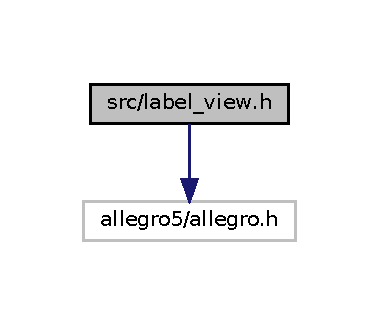
\includegraphics[width=182pt]{label__view_8h__incl}
\end{center}
\end{figure}
Граф файлов, в которые включается этот файл\+:\nopagebreak
\begin{figure}[H]
\begin{center}
\leavevmode
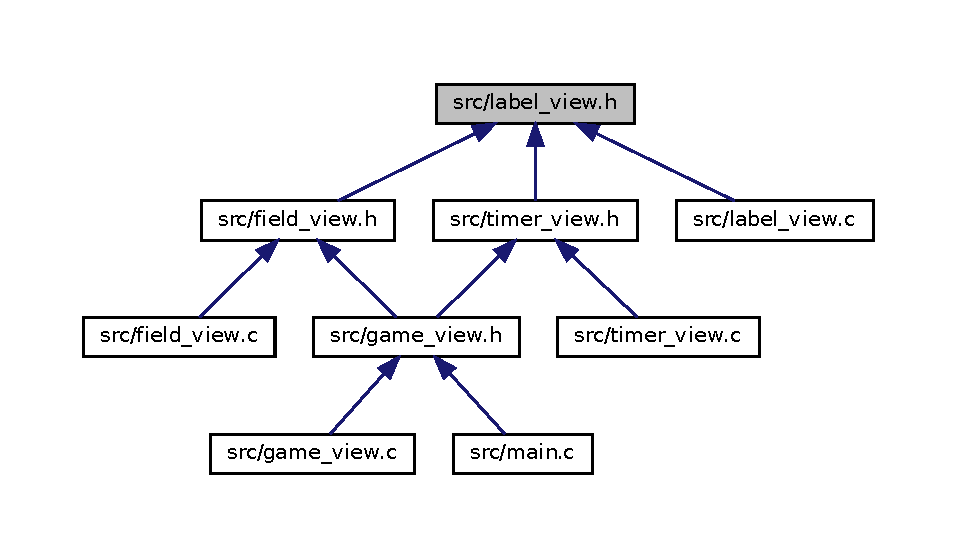
\includegraphics[width=350pt]{label__view_8h__dep__incl}
\end{center}
\end{figure}
\subsection*{Структуры данных}
\begin{DoxyCompactItemize}
\item 
struct \hyperlink{structlabel__view}{label\+\_\+view}
\begin{DoxyCompactList}\small\item\em Структура, которая описывает элемент интерфейса\+: \char`\"{}надпись\char`\"{}. \end{DoxyCompactList}\end{DoxyCompactItemize}
\subsection*{Макросы}
\begin{DoxyCompactItemize}
\item 
\#define \hyperlink{label__view_8h_aae4d8e5464b3520e10b2215db631640b}{M\+A\+X\+\_\+\+L\+E\+N\+\_\+\+T\+E\+XT}~20
\begin{DoxyCompactList}\small\item\em Максимальное количество символов в надписи. \end{DoxyCompactList}\end{DoxyCompactItemize}
\subsection*{Определения типов}
\begin{DoxyCompactItemize}
\item 
typedef struct \hyperlink{structlabel__view}{label\+\_\+view} \hyperlink{label__view_8h_aeeecd1f069a146fc16c68bd327ed09f1}{label\+\_\+view}
\end{DoxyCompactItemize}
\subsection*{Функции}
\begin{DoxyCompactItemize}
\item 
int \hyperlink{label__view_8h_aa0b2902b394029608b3f1cc1bc088f8c}{label\+\_\+view\+\_\+init\+\_\+font} ()
\item 
int \hyperlink{label__view_8h_a22a1e7fc4834fa2f0b0e572889b36ba7}{label\+\_\+view\+\_\+destroy\+\_\+font} ()
\item 
\hyperlink{structlabel__view}{label\+\_\+view} $\ast$ \hyperlink{label__view_8h_a9c2dc97d9adda28c54c27ab98204d82d}{label\+\_\+view\+\_\+create} (const char $\ast$text, unsigned int width, unsigned int height, A\+L\+L\+E\+G\+R\+O\+\_\+\+C\+O\+L\+OR color\+\_\+text, A\+L\+L\+E\+G\+R\+O\+\_\+\+C\+O\+L\+OR color\+\_\+background, A\+L\+L\+E\+G\+R\+O\+\_\+\+C\+O\+L\+OR color\+\_\+border)
\item 
int \hyperlink{label__view_8h_a9e7cb527cf441612379104d571dcfa03}{label\+\_\+view\+\_\+draw} (\hyperlink{structlabel__view}{label\+\_\+view} $\ast$l\+\_\+view, unsigned int x, unsigned int y)
\item 
int \hyperlink{label__view_8h_af2631fe70fdcba7a10ce366577d7c285}{label\+\_\+view\+\_\+set\+\_\+text} (\hyperlink{structlabel__view}{label\+\_\+view} $\ast$l\+\_\+view, const char $\ast$text)
\item 
int \hyperlink{label__view_8h_ad95c787547beb9badc89438681b0b7f4}{label\+\_\+view\+\_\+destroy} (\hyperlink{structlabel__view}{label\+\_\+view} $\ast$l\+\_\+view)
\end{DoxyCompactItemize}


\subsection{Подробное описание}
Файл, в котором опеределены функции для работы с элементом интерфейса\+: \char`\"{}надпись\char`\"{}. 



\subsection{Макросы}
\mbox{\Hypertarget{label__view_8h_aae4d8e5464b3520e10b2215db631640b}\label{label__view_8h_aae4d8e5464b3520e10b2215db631640b}} 
\index{label\+\_\+view.\+h@{label\+\_\+view.\+h}!M\+A\+X\+\_\+\+L\+E\+N\+\_\+\+T\+E\+XT@{M\+A\+X\+\_\+\+L\+E\+N\+\_\+\+T\+E\+XT}}
\index{M\+A\+X\+\_\+\+L\+E\+N\+\_\+\+T\+E\+XT@{M\+A\+X\+\_\+\+L\+E\+N\+\_\+\+T\+E\+XT}!label\+\_\+view.\+h@{label\+\_\+view.\+h}}
\subsubsection{\texorpdfstring{M\+A\+X\+\_\+\+L\+E\+N\+\_\+\+T\+E\+XT}{MAX\_LEN\_TEXT}}
{\footnotesize\ttfamily \#define M\+A\+X\+\_\+\+L\+E\+N\+\_\+\+T\+E\+XT~20}



Максимальное количество символов в надписи. 



\subsection{Типы}
\mbox{\Hypertarget{label__view_8h_aeeecd1f069a146fc16c68bd327ed09f1}\label{label__view_8h_aeeecd1f069a146fc16c68bd327ed09f1}} 
\index{label\+\_\+view.\+h@{label\+\_\+view.\+h}!label\+\_\+view@{label\+\_\+view}}
\index{label\+\_\+view@{label\+\_\+view}!label\+\_\+view.\+h@{label\+\_\+view.\+h}}
\subsubsection{\texorpdfstring{label\+\_\+view}{label\_view}}
{\footnotesize\ttfamily typedef struct \hyperlink{structlabel__view}{label\+\_\+view} \hyperlink{structlabel__view}{label\+\_\+view}}



\subsection{Функции}
\mbox{\Hypertarget{label__view_8h_a9c2dc97d9adda28c54c27ab98204d82d}\label{label__view_8h_a9c2dc97d9adda28c54c27ab98204d82d}} 
\index{label\+\_\+view.\+h@{label\+\_\+view.\+h}!label\+\_\+view\+\_\+create@{label\+\_\+view\+\_\+create}}
\index{label\+\_\+view\+\_\+create@{label\+\_\+view\+\_\+create}!label\+\_\+view.\+h@{label\+\_\+view.\+h}}
\subsubsection{\texorpdfstring{label\+\_\+view\+\_\+create()}{label\_view\_create()}}
{\footnotesize\ttfamily \hyperlink{structlabel__view}{label\+\_\+view}$\ast$ label\+\_\+view\+\_\+create (\begin{DoxyParamCaption}\item[{const char $\ast$}]{text,  }\item[{unsigned int}]{width,  }\item[{unsigned int}]{height,  }\item[{A\+L\+L\+E\+G\+R\+O\+\_\+\+C\+O\+L\+OR}]{color\+\_\+text,  }\item[{A\+L\+L\+E\+G\+R\+O\+\_\+\+C\+O\+L\+OR}]{color\+\_\+background,  }\item[{A\+L\+L\+E\+G\+R\+O\+\_\+\+C\+O\+L\+OR}]{color\+\_\+border }\end{DoxyParamCaption})}

Создание надписи. 
\begin{DoxyParams}[1]{Аргументы}
\mbox{\tt in}  & {\em text} & -\/ текст. \\
\hline
\mbox{\tt in}  & {\em width} & -\/ ширина. \\
\hline
\mbox{\tt in}  & {\em height} & -\/ высота. \\
\hline
\mbox{\tt in}  & {\em color\+\_\+text} & -\/ цвет текста. \\
\hline
\mbox{\tt in}  & {\em color\+\_\+background} & -\/ цвет фона. \\
\hline
\mbox{\tt in}  & {\em color\+\_\+border} & -\/ цвет рамки. \\
\hline
\end{DoxyParams}
\begin{DoxyReturn}{Возвращает}
Адрес, созданной надписи. ~\newline
 N\+U\+LL, если во время создания надписи произошла ошибка. 
\end{DoxyReturn}
\mbox{\Hypertarget{label__view_8h_ad95c787547beb9badc89438681b0b7f4}\label{label__view_8h_ad95c787547beb9badc89438681b0b7f4}} 
\index{label\+\_\+view.\+h@{label\+\_\+view.\+h}!label\+\_\+view\+\_\+destroy@{label\+\_\+view\+\_\+destroy}}
\index{label\+\_\+view\+\_\+destroy@{label\+\_\+view\+\_\+destroy}!label\+\_\+view.\+h@{label\+\_\+view.\+h}}
\subsubsection{\texorpdfstring{label\+\_\+view\+\_\+destroy()}{label\_view\_destroy()}}
{\footnotesize\ttfamily int label\+\_\+view\+\_\+destroy (\begin{DoxyParamCaption}\item[{\hyperlink{structlabel__view}{label\+\_\+view} $\ast$}]{l\+\_\+view }\end{DoxyParamCaption})}

Удаление надписи. 
\begin{DoxyParams}[1]{Аргументы}
\mbox{\tt in}  & {\em l\+\_\+view} & -\/ адрес надписи, которую нужно удалить. \\
\hline
\end{DoxyParams}
\begin{DoxyReturn}{Возвращает}
Ноль, если удаление прошло успешно. ~\newline
 Ненулевое число, если во время удаления произошла ошибка. 
\end{DoxyReturn}
\mbox{\Hypertarget{label__view_8h_a22a1e7fc4834fa2f0b0e572889b36ba7}\label{label__view_8h_a22a1e7fc4834fa2f0b0e572889b36ba7}} 
\index{label\+\_\+view.\+h@{label\+\_\+view.\+h}!label\+\_\+view\+\_\+destroy\+\_\+font@{label\+\_\+view\+\_\+destroy\+\_\+font}}
\index{label\+\_\+view\+\_\+destroy\+\_\+font@{label\+\_\+view\+\_\+destroy\+\_\+font}!label\+\_\+view.\+h@{label\+\_\+view.\+h}}
\subsubsection{\texorpdfstring{label\+\_\+view\+\_\+destroy\+\_\+font()}{label\_view\_destroy\_font()}}
{\footnotesize\ttfamily int label\+\_\+view\+\_\+destroy\+\_\+font (\begin{DoxyParamCaption}{ }\end{DoxyParamCaption})}

Удаление шрифта. \begin{DoxyReturn}{Возвращает}
Ноль, если удаление прошло успешно. ~\newline
 Ненулевое число, если во время удаления произошла ошибка.
\end{DoxyReturn}
\begin{DoxyWarning}{Предупреждения}
Эту функцию обязательно нужно вызвать после удаления всех элементов интерфейса \char`\"{}надпись\char`\"{}. 
\end{DoxyWarning}
\mbox{\Hypertarget{label__view_8h_a9e7cb527cf441612379104d571dcfa03}\label{label__view_8h_a9e7cb527cf441612379104d571dcfa03}} 
\index{label\+\_\+view.\+h@{label\+\_\+view.\+h}!label\+\_\+view\+\_\+draw@{label\+\_\+view\+\_\+draw}}
\index{label\+\_\+view\+\_\+draw@{label\+\_\+view\+\_\+draw}!label\+\_\+view.\+h@{label\+\_\+view.\+h}}
\subsubsection{\texorpdfstring{label\+\_\+view\+\_\+draw()}{label\_view\_draw()}}
{\footnotesize\ttfamily int label\+\_\+view\+\_\+draw (\begin{DoxyParamCaption}\item[{\hyperlink{structlabel__view}{label\+\_\+view} $\ast$}]{l\+\_\+view,  }\item[{unsigned int}]{x,  }\item[{unsigned int}]{y }\end{DoxyParamCaption})}

Рисование надписи. 
\begin{DoxyParams}[1]{Аргументы}
\mbox{\tt in}  & {\em l\+\_\+view} & -\/ адрес надписи, которую нужно нарисовать. \\
\hline
\mbox{\tt in}  & {\em x} & -\/ координата рисования верхнего левого угла надписи по оси OX. \\
\hline
\mbox{\tt in}  & {\em y} & -\/ координата рисования верхнего левого угла надписи по оси OY. \\
\hline
\end{DoxyParams}
\begin{DoxyReturn}{Возвращает}
Ноль, если надпись была успешно отрисована. ~\newline
 Ненулевое число, если во время рисования произошла ошибка. 
\end{DoxyReturn}
\mbox{\Hypertarget{label__view_8h_aa0b2902b394029608b3f1cc1bc088f8c}\label{label__view_8h_aa0b2902b394029608b3f1cc1bc088f8c}} 
\index{label\+\_\+view.\+h@{label\+\_\+view.\+h}!label\+\_\+view\+\_\+init\+\_\+font@{label\+\_\+view\+\_\+init\+\_\+font}}
\index{label\+\_\+view\+\_\+init\+\_\+font@{label\+\_\+view\+\_\+init\+\_\+font}!label\+\_\+view.\+h@{label\+\_\+view.\+h}}
\subsubsection{\texorpdfstring{label\+\_\+view\+\_\+init\+\_\+font()}{label\_view\_init\_font()}}
{\footnotesize\ttfamily int label\+\_\+view\+\_\+init\+\_\+font (\begin{DoxyParamCaption}{ }\end{DoxyParamCaption})}

Инициализация шрифта текстов надписей. \begin{DoxyReturn}{Возвращает}
Ноль, если инифиализация прошла успешно. ~\newline
 Ненулевое число, если во время инициализации произошла ошибка.
\end{DoxyReturn}
\begin{DoxyWarning}{Предупреждения}
Эту функцию обязательно нужно вызвать до создания элементов интерфейса \char`\"{}надпись\char`\"{}. 
\end{DoxyWarning}
\mbox{\Hypertarget{label__view_8h_af2631fe70fdcba7a10ce366577d7c285}\label{label__view_8h_af2631fe70fdcba7a10ce366577d7c285}} 
\index{label\+\_\+view.\+h@{label\+\_\+view.\+h}!label\+\_\+view\+\_\+set\+\_\+text@{label\+\_\+view\+\_\+set\+\_\+text}}
\index{label\+\_\+view\+\_\+set\+\_\+text@{label\+\_\+view\+\_\+set\+\_\+text}!label\+\_\+view.\+h@{label\+\_\+view.\+h}}
\subsubsection{\texorpdfstring{label\+\_\+view\+\_\+set\+\_\+text()}{label\_view\_set\_text()}}
{\footnotesize\ttfamily int label\+\_\+view\+\_\+set\+\_\+text (\begin{DoxyParamCaption}\item[{\hyperlink{structlabel__view}{label\+\_\+view} $\ast$}]{l\+\_\+view,  }\item[{const char $\ast$}]{text }\end{DoxyParamCaption})}

Изменение текста надписи. 
\begin{DoxyParams}[1]{Аргументы}
\mbox{\tt in,out}  & {\em l\+\_\+view} & -\/ адрес надписи, текст которой нужно изменить. \\
\hline
\mbox{\tt in}  & {\em text} & -\/ новый текст надписи. \\
\hline
\end{DoxyParams}
\begin{DoxyReturn}{Возвращает}
Ноль, если текст надписи был успешно изменен. ~\newline
 Ненулевое число, если во время изменения текста произошла ошибка. 
\end{DoxyReturn}

\hypertarget{main_8c}{}\section{Файл src/main.c}
\label{main_8c}\index{src/main.\+c@{src/main.\+c}}


Файл, в котором создается и запускается игра.  


{\ttfamily \#include \char`\"{}game\+\_\+view.\+h\char`\"{}}\newline
{\ttfamily \#include \char`\"{}error\+\_\+report.\+h\char`\"{}}\newline
{\ttfamily \#include $<$allegro5/allegro.\+h$>$}\newline
Граф включаемых заголовочных файлов для main.\+c\+:\nopagebreak
\begin{figure}[H]
\begin{center}
\leavevmode
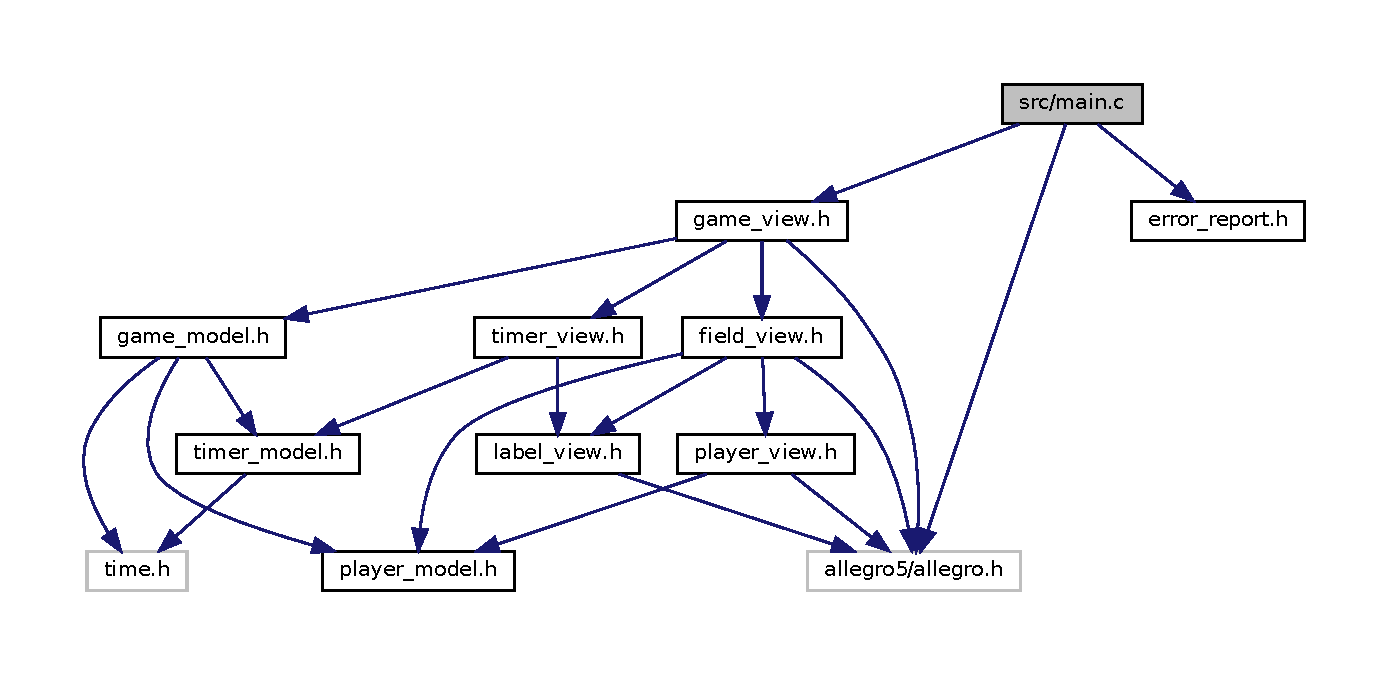
\includegraphics[width=350pt]{main_8c__incl}
\end{center}
\end{figure}
\subsection*{Макросы}
\begin{DoxyCompactItemize}
\item 
\#define \hyperlink{main_8c_ab117546549783a058d0321a287699579}{F\+I\+L\+E\+\_\+\+N\+A\+ME}~\char`\"{}main.\+c\char`\"{}
\begin{DoxyCompactList}\small\item\em Текущие имя файла. \end{DoxyCompactList}\item 
\#define \hyperlink{main_8c_aba64ab31ac50908f7aa4125955fcf2ed}{F\+U\+N\+\_\+\+N\+A\+ME}~\char`\"{}main\char`\"{}
\begin{DoxyCompactList}\small\item\em Имя текущей функции. \end{DoxyCompactList}\end{DoxyCompactItemize}
\subsection*{Функции}
\begin{DoxyCompactItemize}
\item 
int \hyperlink{main_8c_ae66f6b31b5ad750f1fe042a706a4e3d4}{main} ()
\end{DoxyCompactItemize}


\subsection{Подробное описание}
Файл, в котором создается и запускается игра. 



\subsection{Макросы}
\mbox{\Hypertarget{main_8c_ab117546549783a058d0321a287699579}\label{main_8c_ab117546549783a058d0321a287699579}} 
\index{main.\+c@{main.\+c}!F\+I\+L\+E\+\_\+\+N\+A\+ME@{F\+I\+L\+E\+\_\+\+N\+A\+ME}}
\index{F\+I\+L\+E\+\_\+\+N\+A\+ME@{F\+I\+L\+E\+\_\+\+N\+A\+ME}!main.\+c@{main.\+c}}
\subsubsection{\texorpdfstring{F\+I\+L\+E\+\_\+\+N\+A\+ME}{FILE\_NAME}}
{\footnotesize\ttfamily \#define F\+I\+L\+E\+\_\+\+N\+A\+ME~\char`\"{}main.\+c\char`\"{}}



Текущие имя файла. 

\mbox{\Hypertarget{main_8c_aba64ab31ac50908f7aa4125955fcf2ed}\label{main_8c_aba64ab31ac50908f7aa4125955fcf2ed}} 
\index{main.\+c@{main.\+c}!F\+U\+N\+\_\+\+N\+A\+ME@{F\+U\+N\+\_\+\+N\+A\+ME}}
\index{F\+U\+N\+\_\+\+N\+A\+ME@{F\+U\+N\+\_\+\+N\+A\+ME}!main.\+c@{main.\+c}}
\subsubsection{\texorpdfstring{F\+U\+N\+\_\+\+N\+A\+ME}{FUN\_NAME}}
{\footnotesize\ttfamily \#define F\+U\+N\+\_\+\+N\+A\+ME~\char`\"{}main\char`\"{}}



Имя текущей функции. 



\subsection{Функции}
\mbox{\Hypertarget{main_8c_ae66f6b31b5ad750f1fe042a706a4e3d4}\label{main_8c_ae66f6b31b5ad750f1fe042a706a4e3d4}} 
\index{main.\+c@{main.\+c}!main@{main}}
\index{main@{main}!main.\+c@{main.\+c}}
\subsubsection{\texorpdfstring{main()}{main()}}
{\footnotesize\ttfamily int main (\begin{DoxyParamCaption}{ }\end{DoxyParamCaption})}

Точка входа в программу. \begin{DoxyReturn}{Возвращает}
Ноль, если программа успешно завершилась. ~\newline
 Ненулевое число, если в ходе выполнения программы возникла ошибка. 
\end{DoxyReturn}

\hypertarget{player__model_8c}{}\section{Файл src/player\+\_\+model.c}
\label{player__model_8c}\index{src/player\+\_\+model.\+c@{src/player\+\_\+model.\+c}}


Файл, в котором реализованы функции для работы с моделью игрока.  


{\ttfamily \#include \char`\"{}player\+\_\+model.\+h\char`\"{}}\newline
{\ttfamily \#include \char`\"{}error\+\_\+report.\+h\char`\"{}}\newline
{\ttfamily \#include $<$stdlib.\+h$>$}\newline
{\ttfamily \#include $<$math.\+h$>$}\newline
Граф включаемых заголовочных файлов для player\+\_\+model.\+c\+:\nopagebreak
\begin{figure}[H]
\begin{center}
\leavevmode
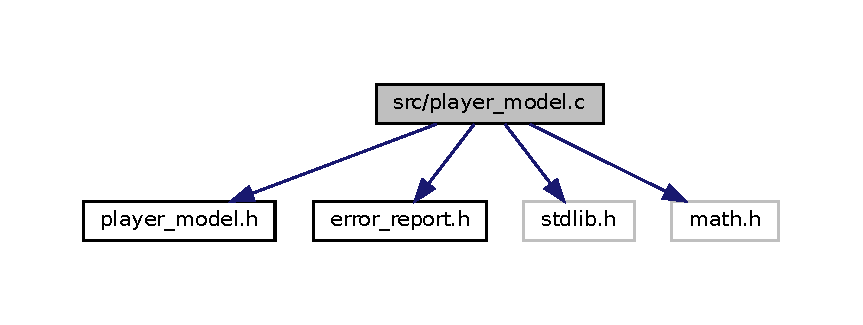
\includegraphics[width=350pt]{player__model_8c__incl}
\end{center}
\end{figure}
\subsection*{Макросы}
\begin{DoxyCompactItemize}
\item 
\#define \hyperlink{player__model_8c_ab117546549783a058d0321a287699579}{F\+I\+L\+E\+\_\+\+N\+A\+ME}~\char`\"{}player\+\_\+model.\+c\char`\"{}
\begin{DoxyCompactList}\small\item\em Имя текущего файла. \end{DoxyCompactList}\item 
\#define \hyperlink{player__model_8c_a6ebf6899d6c1c8b7b9d09be872c05aae}{E\+PS}~1e-\/15
\begin{DoxyCompactList}\small\item\em Точность сравнения вещественных чисел. \end{DoxyCompactList}\item 
\#define \hyperlink{player__model_8c_aba64ab31ac50908f7aa4125955fcf2ed}{F\+U\+N\+\_\+\+N\+A\+ME}~\char`\"{}player\+\_\+model\+\_\+create\char`\"{}
\begin{DoxyCompactList}\small\item\em Имя текущей функции. \end{DoxyCompactList}\item 
\#define \hyperlink{player__model_8c_aba64ab31ac50908f7aa4125955fcf2ed}{F\+U\+N\+\_\+\+N\+A\+ME}~\char`\"{}player\+\_\+model\+\_\+update\char`\"{}
\begin{DoxyCompactList}\small\item\em Имя текущей функции. \end{DoxyCompactList}\item 
\#define \hyperlink{player__model_8c_aba64ab31ac50908f7aa4125955fcf2ed}{F\+U\+N\+\_\+\+N\+A\+ME}~\char`\"{}player\+\_\+model\+\_\+destroy\char`\"{}
\begin{DoxyCompactList}\small\item\em Имя текущей функции. \end{DoxyCompactList}\item 
\#define \hyperlink{player__model_8c_aba64ab31ac50908f7aa4125955fcf2ed}{F\+U\+N\+\_\+\+N\+A\+ME}~\char`\"{}player\+\_\+model\+\_\+is\+\_\+end\char`\"{}
\begin{DoxyCompactList}\small\item\em Имя текущей функции. \end{DoxyCompactList}\end{DoxyCompactItemize}
\subsection*{Функции}
\begin{DoxyCompactItemize}
\item 
\hyperlink{structplayer__model}{player\+\_\+model} $\ast$ \hyperlink{player__model_8c_ab8a395b12df2d231e0b2a4c36f686290}{player\+\_\+model\+\_\+create} ()
\item 
int \hyperlink{player__model_8c_a56743d09659282cdc60c27f16028036e}{player\+\_\+model\+\_\+update} (\hyperlink{structplayer__model}{player\+\_\+model} $\ast$p\+\_\+model, double speed)
\item 
int \hyperlink{player__model_8c_aab36afe2a7a3311da59ee784ecc7548f}{player\+\_\+model\+\_\+destroy} (\hyperlink{structplayer__model}{player\+\_\+model} $\ast$p\+\_\+model)
\item 
int \hyperlink{player__model_8c_a9014984955be35c6de7f854c5c439980}{player\+\_\+model\+\_\+is\+\_\+end} (\hyperlink{structplayer__model}{player\+\_\+model} $\ast$p\+\_\+model)
\end{DoxyCompactItemize}


\subsection{Подробное описание}
Файл, в котором реализованы функции для работы с моделью игрока. 



\subsection{Макросы}
\mbox{\Hypertarget{player__model_8c_a6ebf6899d6c1c8b7b9d09be872c05aae}\label{player__model_8c_a6ebf6899d6c1c8b7b9d09be872c05aae}} 
\index{player\+\_\+model.\+c@{player\+\_\+model.\+c}!E\+PS@{E\+PS}}
\index{E\+PS@{E\+PS}!player\+\_\+model.\+c@{player\+\_\+model.\+c}}
\subsubsection{\texorpdfstring{E\+PS}{EPS}}
{\footnotesize\ttfamily \#define E\+PS~1e-\/15}



Точность сравнения вещественных чисел. 

\mbox{\Hypertarget{player__model_8c_ab117546549783a058d0321a287699579}\label{player__model_8c_ab117546549783a058d0321a287699579}} 
\index{player\+\_\+model.\+c@{player\+\_\+model.\+c}!F\+I\+L\+E\+\_\+\+N\+A\+ME@{F\+I\+L\+E\+\_\+\+N\+A\+ME}}
\index{F\+I\+L\+E\+\_\+\+N\+A\+ME@{F\+I\+L\+E\+\_\+\+N\+A\+ME}!player\+\_\+model.\+c@{player\+\_\+model.\+c}}
\subsubsection{\texorpdfstring{F\+I\+L\+E\+\_\+\+N\+A\+ME}{FILE\_NAME}}
{\footnotesize\ttfamily \#define F\+I\+L\+E\+\_\+\+N\+A\+ME~\char`\"{}player\+\_\+model.\+c\char`\"{}}



Имя текущего файла. 

\mbox{\Hypertarget{player__model_8c_aba64ab31ac50908f7aa4125955fcf2ed}\label{player__model_8c_aba64ab31ac50908f7aa4125955fcf2ed}} 
\index{player\+\_\+model.\+c@{player\+\_\+model.\+c}!F\+U\+N\+\_\+\+N\+A\+ME@{F\+U\+N\+\_\+\+N\+A\+ME}}
\index{F\+U\+N\+\_\+\+N\+A\+ME@{F\+U\+N\+\_\+\+N\+A\+ME}!player\+\_\+model.\+c@{player\+\_\+model.\+c}}
\subsubsection{\texorpdfstring{F\+U\+N\+\_\+\+N\+A\+ME}{FUN\_NAME}\hspace{0.1cm}{\footnotesize\ttfamily [1/4]}}
{\footnotesize\ttfamily \#define F\+U\+N\+\_\+\+N\+A\+ME~\char`\"{}player\+\_\+model\+\_\+create\char`\"{}}



Имя текущей функции. 

\mbox{\Hypertarget{player__model_8c_aba64ab31ac50908f7aa4125955fcf2ed}\label{player__model_8c_aba64ab31ac50908f7aa4125955fcf2ed}} 
\index{player\+\_\+model.\+c@{player\+\_\+model.\+c}!F\+U\+N\+\_\+\+N\+A\+ME@{F\+U\+N\+\_\+\+N\+A\+ME}}
\index{F\+U\+N\+\_\+\+N\+A\+ME@{F\+U\+N\+\_\+\+N\+A\+ME}!player\+\_\+model.\+c@{player\+\_\+model.\+c}}
\subsubsection{\texorpdfstring{F\+U\+N\+\_\+\+N\+A\+ME}{FUN\_NAME}\hspace{0.1cm}{\footnotesize\ttfamily [2/4]}}
{\footnotesize\ttfamily \#define F\+U\+N\+\_\+\+N\+A\+ME~\char`\"{}player\+\_\+model\+\_\+update\char`\"{}}



Имя текущей функции. 

\mbox{\Hypertarget{player__model_8c_aba64ab31ac50908f7aa4125955fcf2ed}\label{player__model_8c_aba64ab31ac50908f7aa4125955fcf2ed}} 
\index{player\+\_\+model.\+c@{player\+\_\+model.\+c}!F\+U\+N\+\_\+\+N\+A\+ME@{F\+U\+N\+\_\+\+N\+A\+ME}}
\index{F\+U\+N\+\_\+\+N\+A\+ME@{F\+U\+N\+\_\+\+N\+A\+ME}!player\+\_\+model.\+c@{player\+\_\+model.\+c}}
\subsubsection{\texorpdfstring{F\+U\+N\+\_\+\+N\+A\+ME}{FUN\_NAME}\hspace{0.1cm}{\footnotesize\ttfamily [3/4]}}
{\footnotesize\ttfamily \#define F\+U\+N\+\_\+\+N\+A\+ME~\char`\"{}player\+\_\+model\+\_\+destroy\char`\"{}}



Имя текущей функции. 

\mbox{\Hypertarget{player__model_8c_aba64ab31ac50908f7aa4125955fcf2ed}\label{player__model_8c_aba64ab31ac50908f7aa4125955fcf2ed}} 
\index{player\+\_\+model.\+c@{player\+\_\+model.\+c}!F\+U\+N\+\_\+\+N\+A\+ME@{F\+U\+N\+\_\+\+N\+A\+ME}}
\index{F\+U\+N\+\_\+\+N\+A\+ME@{F\+U\+N\+\_\+\+N\+A\+ME}!player\+\_\+model.\+c@{player\+\_\+model.\+c}}
\subsubsection{\texorpdfstring{F\+U\+N\+\_\+\+N\+A\+ME}{FUN\_NAME}\hspace{0.1cm}{\footnotesize\ttfamily [4/4]}}
{\footnotesize\ttfamily \#define F\+U\+N\+\_\+\+N\+A\+ME~\char`\"{}player\+\_\+model\+\_\+is\+\_\+end\char`\"{}}



Имя текущей функции. 



\subsection{Функции}
\mbox{\Hypertarget{player__model_8c_ab8a395b12df2d231e0b2a4c36f686290}\label{player__model_8c_ab8a395b12df2d231e0b2a4c36f686290}} 
\index{player\+\_\+model.\+c@{player\+\_\+model.\+c}!player\+\_\+model\+\_\+create@{player\+\_\+model\+\_\+create}}
\index{player\+\_\+model\+\_\+create@{player\+\_\+model\+\_\+create}!player\+\_\+model.\+c@{player\+\_\+model.\+c}}
\subsubsection{\texorpdfstring{player\+\_\+model\+\_\+create()}{player\_model\_create()}}
{\footnotesize\ttfamily \hyperlink{structplayer__model}{player\+\_\+model}$\ast$ player\+\_\+model\+\_\+create (\begin{DoxyParamCaption}{ }\end{DoxyParamCaption})}

Создание модели игрока. \begin{DoxyReturn}{Возвращает}
Адрес, созданной модели. ~\newline
 N\+U\+LL, если во время создания модели произошла ошибка. 
\end{DoxyReturn}
\mbox{\Hypertarget{player__model_8c_aab36afe2a7a3311da59ee784ecc7548f}\label{player__model_8c_aab36afe2a7a3311da59ee784ecc7548f}} 
\index{player\+\_\+model.\+c@{player\+\_\+model.\+c}!player\+\_\+model\+\_\+destroy@{player\+\_\+model\+\_\+destroy}}
\index{player\+\_\+model\+\_\+destroy@{player\+\_\+model\+\_\+destroy}!player\+\_\+model.\+c@{player\+\_\+model.\+c}}
\subsubsection{\texorpdfstring{player\+\_\+model\+\_\+destroy()}{player\_model\_destroy()}}
{\footnotesize\ttfamily int player\+\_\+model\+\_\+destroy (\begin{DoxyParamCaption}\item[{\hyperlink{structplayer__model}{player\+\_\+model} $\ast$}]{p\+\_\+model }\end{DoxyParamCaption})}

Удаление модели игрока. 
\begin{DoxyParams}[1]{Аргументы}
\mbox{\tt in,out}  & {\em p\+\_\+model} & -\/ адрес модели игрока, которую необходимо удалить. \\
\hline
\end{DoxyParams}
\begin{DoxyReturn}{Возвращает}
Ноль, если удаление прошло успешно. ~\newline
 Ненулевое число, если во время удаления произошла ошибка. 
\end{DoxyReturn}
\mbox{\Hypertarget{player__model_8c_a9014984955be35c6de7f854c5c439980}\label{player__model_8c_a9014984955be35c6de7f854c5c439980}} 
\index{player\+\_\+model.\+c@{player\+\_\+model.\+c}!player\+\_\+model\+\_\+is\+\_\+end@{player\+\_\+model\+\_\+is\+\_\+end}}
\index{player\+\_\+model\+\_\+is\+\_\+end@{player\+\_\+model\+\_\+is\+\_\+end}!player\+\_\+model.\+c@{player\+\_\+model.\+c}}
\subsubsection{\texorpdfstring{player\+\_\+model\+\_\+is\+\_\+end()}{player\_model\_is\_end()}}
{\footnotesize\ttfamily int player\+\_\+model\+\_\+is\+\_\+end (\begin{DoxyParamCaption}\item[{\hyperlink{structplayer__model}{player\+\_\+model} $\ast$}]{p\+\_\+model }\end{DoxyParamCaption})}

Проверка прохождения игроком всей дистанции. 
\begin{DoxyParams}[1]{Аргументы}
\mbox{\tt in}  & {\em p\+\_\+model} & -\/ адрес модели игрока, данные которой небходимо проверить. \\
\hline
\end{DoxyParams}
\begin{DoxyReturn}{Возвращает}
Отрицательное число, если во время проверки произошла ошибка. ~\newline
 Ноль, если игрок не прошел дистанцию. ~\newline
 Положительное число, если игрок прошел дистанцию. 
\end{DoxyReturn}
\mbox{\Hypertarget{player__model_8c_a56743d09659282cdc60c27f16028036e}\label{player__model_8c_a56743d09659282cdc60c27f16028036e}} 
\index{player\+\_\+model.\+c@{player\+\_\+model.\+c}!player\+\_\+model\+\_\+update@{player\+\_\+model\+\_\+update}}
\index{player\+\_\+model\+\_\+update@{player\+\_\+model\+\_\+update}!player\+\_\+model.\+c@{player\+\_\+model.\+c}}
\subsubsection{\texorpdfstring{player\+\_\+model\+\_\+update()}{player\_model\_update()}}
{\footnotesize\ttfamily int player\+\_\+model\+\_\+update (\begin{DoxyParamCaption}\item[{\hyperlink{structplayer__model}{player\+\_\+model} $\ast$}]{p\+\_\+model,  }\item[{double}]{speed }\end{DoxyParamCaption})}

Обновление данных модели игрока. 
\begin{DoxyParams}[1]{Аргументы}
\mbox{\tt in,out}  & {\em p\+\_\+model} & -\/ адрес модели игрока, которую необходимо обновить. \\
\hline
\mbox{\tt in}  & {\em speed} & -\/ текущая скорость игрока. \\
\hline
\end{DoxyParams}
\begin{DoxyReturn}{Возвращает}
Ноль, если обновление прошло успешно. ~\newline
 Ненулевое число, если во время обновления произошла ошибка. 
\end{DoxyReturn}

\hypertarget{player__model_8h}{}\section{Файл src/player\+\_\+model.h}
\label{player__model_8h}\index{src/player\+\_\+model.\+h@{src/player\+\_\+model.\+h}}


Файл, в котором опеределены функции для работы с моделью игрока.  


Граф файлов, в которые включается этот файл\+:\nopagebreak
\begin{figure}[H]
\begin{center}
\leavevmode
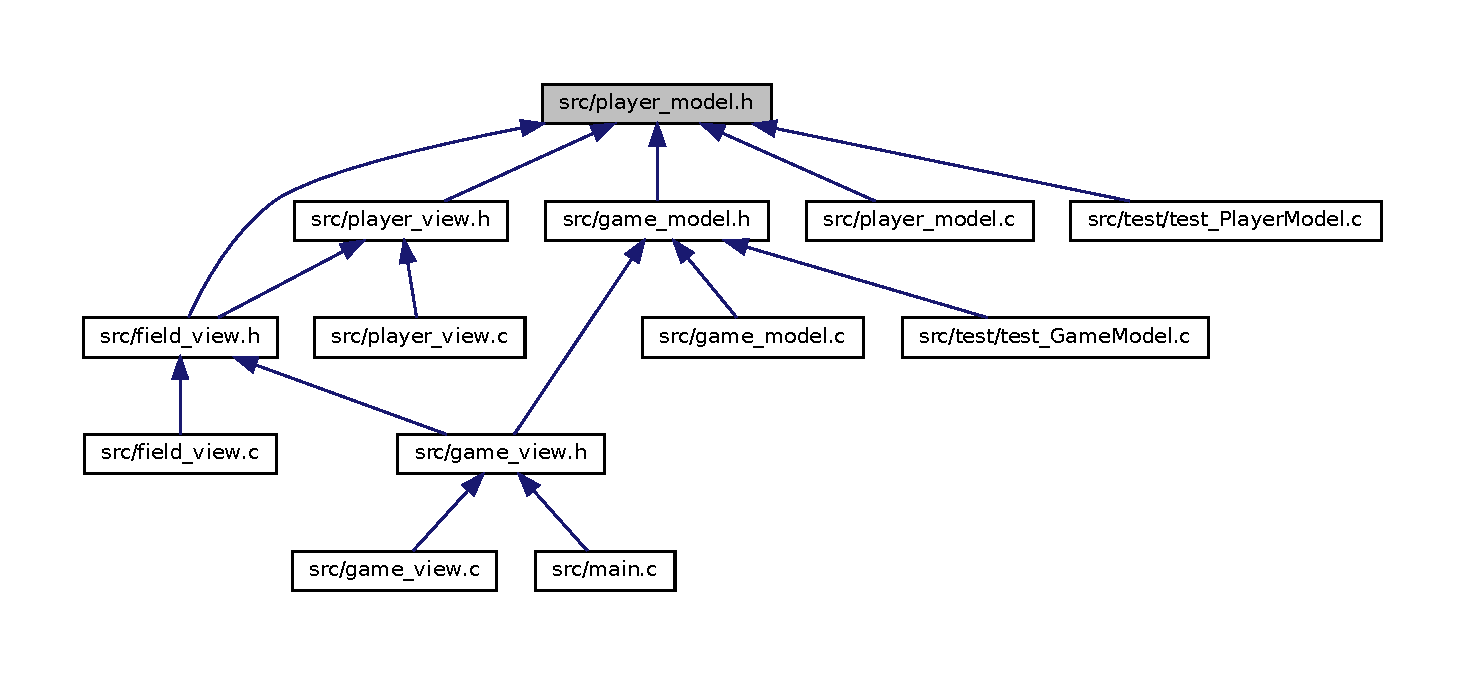
\includegraphics[width=350pt]{player__model_8h__dep__incl}
\end{center}
\end{figure}
\subsection*{Структуры данных}
\begin{DoxyCompactItemize}
\item 
struct \hyperlink{structplayer__model}{player\+\_\+model}
\begin{DoxyCompactList}\small\item\em Структура, которая описывает модель игрока. \end{DoxyCompactList}\end{DoxyCompactItemize}
\subsection*{Макросы}
\begin{DoxyCompactItemize}
\item 
\#define \hyperlink{player__model_8h_a48e09d724ad8d412d3b973902199d372}{D\+I\+S\+T\+A\+N\+C\+E\+\_\+\+L\+E\+N\+G\+TH}~1000
\begin{DoxyCompactList}\small\item\em Дистанция, которую должен пройти игрок. \end{DoxyCompactList}\item 
\#define \hyperlink{player__model_8h_ac2cd96d53dd3ba6407db6766c3d92b26}{M\+A\+X\+\_\+\+S\+P\+E\+ED}~1000
\begin{DoxyCompactList}\small\item\em Максимальная скорость игрока. \end{DoxyCompactList}\end{DoxyCompactItemize}
\subsection*{Определения типов}
\begin{DoxyCompactItemize}
\item 
typedef struct \hyperlink{structplayer__model}{player\+\_\+model} \hyperlink{player__model_8h_a2fe32cb1845e33e3d98460f114486323}{player\+\_\+model}
\end{DoxyCompactItemize}
\subsection*{Функции}
\begin{DoxyCompactItemize}
\item 
\hyperlink{structplayer__model}{player\+\_\+model} $\ast$ \hyperlink{player__model_8h_ab8a395b12df2d231e0b2a4c36f686290}{player\+\_\+model\+\_\+create} ()
\item 
int \hyperlink{player__model_8h_a56743d09659282cdc60c27f16028036e}{player\+\_\+model\+\_\+update} (\hyperlink{structplayer__model}{player\+\_\+model} $\ast$p\+\_\+model, double speed)
\item 
int \hyperlink{player__model_8h_aab36afe2a7a3311da59ee784ecc7548f}{player\+\_\+model\+\_\+destroy} (\hyperlink{structplayer__model}{player\+\_\+model} $\ast$p\+\_\+model)
\item 
int \hyperlink{player__model_8h_a9014984955be35c6de7f854c5c439980}{player\+\_\+model\+\_\+is\+\_\+end} (\hyperlink{structplayer__model}{player\+\_\+model} $\ast$p\+\_\+model)
\end{DoxyCompactItemize}


\subsection{Подробное описание}
Файл, в котором опеределены функции для работы с моделью игрока. 



\subsection{Макросы}
\mbox{\Hypertarget{player__model_8h_a48e09d724ad8d412d3b973902199d372}\label{player__model_8h_a48e09d724ad8d412d3b973902199d372}} 
\index{player\+\_\+model.\+h@{player\+\_\+model.\+h}!D\+I\+S\+T\+A\+N\+C\+E\+\_\+\+L\+E\+N\+G\+TH@{D\+I\+S\+T\+A\+N\+C\+E\+\_\+\+L\+E\+N\+G\+TH}}
\index{D\+I\+S\+T\+A\+N\+C\+E\+\_\+\+L\+E\+N\+G\+TH@{D\+I\+S\+T\+A\+N\+C\+E\+\_\+\+L\+E\+N\+G\+TH}!player\+\_\+model.\+h@{player\+\_\+model.\+h}}
\subsubsection{\texorpdfstring{D\+I\+S\+T\+A\+N\+C\+E\+\_\+\+L\+E\+N\+G\+TH}{DISTANCE\_LENGTH}}
{\footnotesize\ttfamily \#define D\+I\+S\+T\+A\+N\+C\+E\+\_\+\+L\+E\+N\+G\+TH~1000}



Дистанция, которую должен пройти игрок. 

\mbox{\Hypertarget{player__model_8h_ac2cd96d53dd3ba6407db6766c3d92b26}\label{player__model_8h_ac2cd96d53dd3ba6407db6766c3d92b26}} 
\index{player\+\_\+model.\+h@{player\+\_\+model.\+h}!M\+A\+X\+\_\+\+S\+P\+E\+ED@{M\+A\+X\+\_\+\+S\+P\+E\+ED}}
\index{M\+A\+X\+\_\+\+S\+P\+E\+ED@{M\+A\+X\+\_\+\+S\+P\+E\+ED}!player\+\_\+model.\+h@{player\+\_\+model.\+h}}
\subsubsection{\texorpdfstring{M\+A\+X\+\_\+\+S\+P\+E\+ED}{MAX\_SPEED}}
{\footnotesize\ttfamily \#define M\+A\+X\+\_\+\+S\+P\+E\+ED~1000}



Максимальная скорость игрока. 



\subsection{Типы}
\mbox{\Hypertarget{player__model_8h_a2fe32cb1845e33e3d98460f114486323}\label{player__model_8h_a2fe32cb1845e33e3d98460f114486323}} 
\index{player\+\_\+model.\+h@{player\+\_\+model.\+h}!player\+\_\+model@{player\+\_\+model}}
\index{player\+\_\+model@{player\+\_\+model}!player\+\_\+model.\+h@{player\+\_\+model.\+h}}
\subsubsection{\texorpdfstring{player\+\_\+model}{player\_model}}
{\footnotesize\ttfamily typedef struct \hyperlink{structplayer__model}{player\+\_\+model} \hyperlink{structplayer__model}{player\+\_\+model}}



\subsection{Функции}
\mbox{\Hypertarget{player__model_8h_ab8a395b12df2d231e0b2a4c36f686290}\label{player__model_8h_ab8a395b12df2d231e0b2a4c36f686290}} 
\index{player\+\_\+model.\+h@{player\+\_\+model.\+h}!player\+\_\+model\+\_\+create@{player\+\_\+model\+\_\+create}}
\index{player\+\_\+model\+\_\+create@{player\+\_\+model\+\_\+create}!player\+\_\+model.\+h@{player\+\_\+model.\+h}}
\subsubsection{\texorpdfstring{player\+\_\+model\+\_\+create()}{player\_model\_create()}}
{\footnotesize\ttfamily \hyperlink{structplayer__model}{player\+\_\+model}$\ast$ player\+\_\+model\+\_\+create (\begin{DoxyParamCaption}{ }\end{DoxyParamCaption})}

Создание модели игрока. \begin{DoxyReturn}{Возвращает}
Адрес, созданной модели. ~\newline
 N\+U\+LL, если во время создания модели произошла ошибка. 
\end{DoxyReturn}
\mbox{\Hypertarget{player__model_8h_aab36afe2a7a3311da59ee784ecc7548f}\label{player__model_8h_aab36afe2a7a3311da59ee784ecc7548f}} 
\index{player\+\_\+model.\+h@{player\+\_\+model.\+h}!player\+\_\+model\+\_\+destroy@{player\+\_\+model\+\_\+destroy}}
\index{player\+\_\+model\+\_\+destroy@{player\+\_\+model\+\_\+destroy}!player\+\_\+model.\+h@{player\+\_\+model.\+h}}
\subsubsection{\texorpdfstring{player\+\_\+model\+\_\+destroy()}{player\_model\_destroy()}}
{\footnotesize\ttfamily int player\+\_\+model\+\_\+destroy (\begin{DoxyParamCaption}\item[{\hyperlink{structplayer__model}{player\+\_\+model} $\ast$}]{p\+\_\+model }\end{DoxyParamCaption})}

Удаление модели игрока. 
\begin{DoxyParams}[1]{Аргументы}
\mbox{\tt in,out}  & {\em p\+\_\+model} & -\/ адрес модели игрока, которую необходимо удалить. \\
\hline
\end{DoxyParams}
\begin{DoxyReturn}{Возвращает}
Ноль, если удаление прошло успешно. ~\newline
 Ненулевое число, если во время удаления произошла ошибка. 
\end{DoxyReturn}
\mbox{\Hypertarget{player__model_8h_a9014984955be35c6de7f854c5c439980}\label{player__model_8h_a9014984955be35c6de7f854c5c439980}} 
\index{player\+\_\+model.\+h@{player\+\_\+model.\+h}!player\+\_\+model\+\_\+is\+\_\+end@{player\+\_\+model\+\_\+is\+\_\+end}}
\index{player\+\_\+model\+\_\+is\+\_\+end@{player\+\_\+model\+\_\+is\+\_\+end}!player\+\_\+model.\+h@{player\+\_\+model.\+h}}
\subsubsection{\texorpdfstring{player\+\_\+model\+\_\+is\+\_\+end()}{player\_model\_is\_end()}}
{\footnotesize\ttfamily int player\+\_\+model\+\_\+is\+\_\+end (\begin{DoxyParamCaption}\item[{\hyperlink{structplayer__model}{player\+\_\+model} $\ast$}]{p\+\_\+model }\end{DoxyParamCaption})}

Проверка прохождения игроком всей дистанции. 
\begin{DoxyParams}[1]{Аргументы}
\mbox{\tt in}  & {\em p\+\_\+model} & -\/ адрес модели игрока, данные которой небходимо проверить. \\
\hline
\end{DoxyParams}
\begin{DoxyReturn}{Возвращает}
Отрицательное число, если во время проверки произошла ошибка. ~\newline
 Ноль, если игрок не прошел дистанцию. ~\newline
 Положительное число, если игрок прошел дистанцию. 
\end{DoxyReturn}
\mbox{\Hypertarget{player__model_8h_a56743d09659282cdc60c27f16028036e}\label{player__model_8h_a56743d09659282cdc60c27f16028036e}} 
\index{player\+\_\+model.\+h@{player\+\_\+model.\+h}!player\+\_\+model\+\_\+update@{player\+\_\+model\+\_\+update}}
\index{player\+\_\+model\+\_\+update@{player\+\_\+model\+\_\+update}!player\+\_\+model.\+h@{player\+\_\+model.\+h}}
\subsubsection{\texorpdfstring{player\+\_\+model\+\_\+update()}{player\_model\_update()}}
{\footnotesize\ttfamily int player\+\_\+model\+\_\+update (\begin{DoxyParamCaption}\item[{\hyperlink{structplayer__model}{player\+\_\+model} $\ast$}]{p\+\_\+model,  }\item[{double}]{speed }\end{DoxyParamCaption})}

Обновление данных модели игрока. 
\begin{DoxyParams}[1]{Аргументы}
\mbox{\tt in,out}  & {\em p\+\_\+model} & -\/ адрес модели игрока, которую необходимо обновить. \\
\hline
\mbox{\tt in}  & {\em speed} & -\/ текущая скорость игрока. \\
\hline
\end{DoxyParams}
\begin{DoxyReturn}{Возвращает}
Ноль, если обновление прошло успешно. ~\newline
 Ненулевое число, если во время обновления произошла ошибка. 
\end{DoxyReturn}

\hypertarget{player__view_8c}{}\section{Файл src/player\+\_\+view.c}
\label{player__view_8c}\index{src/player\+\_\+view.\+c@{src/player\+\_\+view.\+c}}
{\ttfamily \#include \char`\"{}player\+\_\+view.\+h\char`\"{}}\newline
{\ttfamily \#include \char`\"{}rectangle\+\_\+view.\+h\char`\"{}}\newline
{\ttfamily \#include \char`\"{}error\+\_\+report.\+h\char`\"{}}\newline
{\ttfamily \#include $<$stdlib.\+h$>$}\newline
Граф включаемых заголовочных файлов для player\+\_\+view.\+c\+:\nopagebreak
\begin{figure}[H]
\begin{center}
\leavevmode
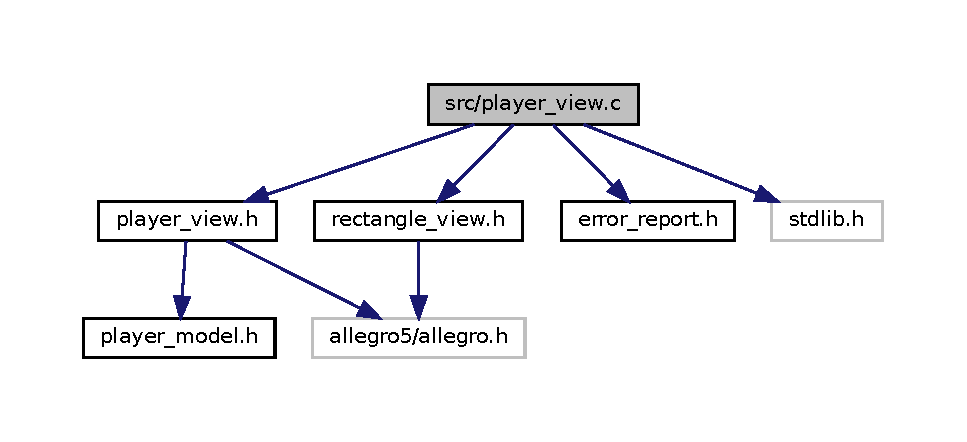
\includegraphics[width=350pt]{player__view_8c__incl}
\end{center}
\end{figure}
\subsection*{Макросы}
\begin{DoxyCompactItemize}
\item 
\#define \hyperlink{player__view_8c_ab117546549783a058d0321a287699579}{F\+I\+L\+E\+\_\+\+N\+A\+ME}~\char`\"{}player\+\_\+view.\+c\char`\"{}
\begin{DoxyCompactList}\small\item\em Имя текущего файла. \end{DoxyCompactList}\item 
\#define \hyperlink{player__view_8c_a6a010865b10e541735fa2da8f3cd062d}{abs}(a)~(((a) $>$ 0) ? (a) \+: (-\/(a)))
\begin{DoxyCompactList}\small\item\em Макрос для нахождение модуля аргумента. \end{DoxyCompactList}\item 
\#define \hyperlink{player__view_8c_aba64ab31ac50908f7aa4125955fcf2ed}{F\+U\+N\+\_\+\+N\+A\+ME}~\char`\"{}player\+\_\+view\+\_\+create\char`\"{}
\begin{DoxyCompactList}\small\item\em Имя текущей функции. \end{DoxyCompactList}\item 
\#define \hyperlink{player__view_8c_aba64ab31ac50908f7aa4125955fcf2ed}{F\+U\+N\+\_\+\+N\+A\+ME}~\char`\"{}player\+\_\+view\+\_\+draw\char`\"{}
\begin{DoxyCompactList}\small\item\em Имя текущей функции. \end{DoxyCompactList}\item 
\#define \hyperlink{player__view_8c_aba64ab31ac50908f7aa4125955fcf2ed}{F\+U\+N\+\_\+\+N\+A\+ME}~\char`\"{}player\+\_\+view\+\_\+destroy\char`\"{}
\begin{DoxyCompactList}\small\item\em Имя текущей функции. \end{DoxyCompactList}\end{DoxyCompactItemize}
\subsection*{Функции}
\begin{DoxyCompactItemize}
\item 
\hyperlink{structplayer__view}{player\+\_\+view} $\ast$ \hyperlink{player__view_8c_ad29d725f51acc28e6b284f0e124be650}{player\+\_\+view\+\_\+create} (\hyperlink{structplayer__model}{player\+\_\+model} $\ast$p\+\_\+model, unsigned int x\+\_\+start, unsigned int y\+\_\+start, unsigned int y\+\_\+finish)
\item 
int \hyperlink{player__view_8c_aabc16f780865d02b2f8a4f7719616cf1}{player\+\_\+view\+\_\+draw} (\hyperlink{structplayer__view}{player\+\_\+view} $\ast$p\+\_\+view)
\item 
int \hyperlink{player__view_8c_a8e15be2eea78a0500de34ac3773a1ed8}{player\+\_\+view\+\_\+destroy} (\hyperlink{structplayer__view}{player\+\_\+view} $\ast$p\+\_\+view)
\end{DoxyCompactItemize}


\subsection{Макросы}
\mbox{\Hypertarget{player__view_8c_a6a010865b10e541735fa2da8f3cd062d}\label{player__view_8c_a6a010865b10e541735fa2da8f3cd062d}} 
\index{player\+\_\+view.\+c@{player\+\_\+view.\+c}!abs@{abs}}
\index{abs@{abs}!player\+\_\+view.\+c@{player\+\_\+view.\+c}}
\subsubsection{\texorpdfstring{abs}{abs}}
{\footnotesize\ttfamily \#define abs(\begin{DoxyParamCaption}\item[{}]{a }\end{DoxyParamCaption})~(((a) $>$ 0) ? (a) \+: (-\/(a)))}



Макрос для нахождение модуля аргумента. 

\mbox{\Hypertarget{player__view_8c_ab117546549783a058d0321a287699579}\label{player__view_8c_ab117546549783a058d0321a287699579}} 
\index{player\+\_\+view.\+c@{player\+\_\+view.\+c}!F\+I\+L\+E\+\_\+\+N\+A\+ME@{F\+I\+L\+E\+\_\+\+N\+A\+ME}}
\index{F\+I\+L\+E\+\_\+\+N\+A\+ME@{F\+I\+L\+E\+\_\+\+N\+A\+ME}!player\+\_\+view.\+c@{player\+\_\+view.\+c}}
\subsubsection{\texorpdfstring{F\+I\+L\+E\+\_\+\+N\+A\+ME}{FILE\_NAME}}
{\footnotesize\ttfamily \#define F\+I\+L\+E\+\_\+\+N\+A\+ME~\char`\"{}player\+\_\+view.\+c\char`\"{}}



Имя текущего файла. 

\mbox{\Hypertarget{player__view_8c_aba64ab31ac50908f7aa4125955fcf2ed}\label{player__view_8c_aba64ab31ac50908f7aa4125955fcf2ed}} 
\index{player\+\_\+view.\+c@{player\+\_\+view.\+c}!F\+U\+N\+\_\+\+N\+A\+ME@{F\+U\+N\+\_\+\+N\+A\+ME}}
\index{F\+U\+N\+\_\+\+N\+A\+ME@{F\+U\+N\+\_\+\+N\+A\+ME}!player\+\_\+view.\+c@{player\+\_\+view.\+c}}
\subsubsection{\texorpdfstring{F\+U\+N\+\_\+\+N\+A\+ME}{FUN\_NAME}\hspace{0.1cm}{\footnotesize\ttfamily [1/3]}}
{\footnotesize\ttfamily \#define F\+U\+N\+\_\+\+N\+A\+ME~\char`\"{}player\+\_\+view\+\_\+create\char`\"{}}



Имя текущей функции. 

\mbox{\Hypertarget{player__view_8c_aba64ab31ac50908f7aa4125955fcf2ed}\label{player__view_8c_aba64ab31ac50908f7aa4125955fcf2ed}} 
\index{player\+\_\+view.\+c@{player\+\_\+view.\+c}!F\+U\+N\+\_\+\+N\+A\+ME@{F\+U\+N\+\_\+\+N\+A\+ME}}
\index{F\+U\+N\+\_\+\+N\+A\+ME@{F\+U\+N\+\_\+\+N\+A\+ME}!player\+\_\+view.\+c@{player\+\_\+view.\+c}}
\subsubsection{\texorpdfstring{F\+U\+N\+\_\+\+N\+A\+ME}{FUN\_NAME}\hspace{0.1cm}{\footnotesize\ttfamily [2/3]}}
{\footnotesize\ttfamily \#define F\+U\+N\+\_\+\+N\+A\+ME~\char`\"{}player\+\_\+view\+\_\+draw\char`\"{}}



Имя текущей функции. 

\mbox{\Hypertarget{player__view_8c_aba64ab31ac50908f7aa4125955fcf2ed}\label{player__view_8c_aba64ab31ac50908f7aa4125955fcf2ed}} 
\index{player\+\_\+view.\+c@{player\+\_\+view.\+c}!F\+U\+N\+\_\+\+N\+A\+ME@{F\+U\+N\+\_\+\+N\+A\+ME}}
\index{F\+U\+N\+\_\+\+N\+A\+ME@{F\+U\+N\+\_\+\+N\+A\+ME}!player\+\_\+view.\+c@{player\+\_\+view.\+c}}
\subsubsection{\texorpdfstring{F\+U\+N\+\_\+\+N\+A\+ME}{FUN\_NAME}\hspace{0.1cm}{\footnotesize\ttfamily [3/3]}}
{\footnotesize\ttfamily \#define F\+U\+N\+\_\+\+N\+A\+ME~\char`\"{}player\+\_\+view\+\_\+destroy\char`\"{}}



Имя текущей функции. 



\subsection{Функции}
\mbox{\Hypertarget{player__view_8c_ad29d725f51acc28e6b284f0e124be650}\label{player__view_8c_ad29d725f51acc28e6b284f0e124be650}} 
\index{player\+\_\+view.\+c@{player\+\_\+view.\+c}!player\+\_\+view\+\_\+create@{player\+\_\+view\+\_\+create}}
\index{player\+\_\+view\+\_\+create@{player\+\_\+view\+\_\+create}!player\+\_\+view.\+c@{player\+\_\+view.\+c}}
\subsubsection{\texorpdfstring{player\+\_\+view\+\_\+create()}{player\_view\_create()}}
{\footnotesize\ttfamily \hyperlink{structplayer__view}{player\+\_\+view}$\ast$ player\+\_\+view\+\_\+create (\begin{DoxyParamCaption}\item[{\hyperlink{structplayer__model}{player\+\_\+model} $\ast$}]{p\+\_\+model,  }\item[{unsigned int}]{x\+\_\+start,  }\item[{unsigned int}]{y\+\_\+start,  }\item[{unsigned int}]{y\+\_\+finish }\end{DoxyParamCaption})}

Создание отображения игрока. 
\begin{DoxyParams}[1]{Аргументы}
\mbox{\tt in}  & {\em p\+\_\+model} & -\/ адрес модели игрока. \\
\hline
\mbox{\tt in}  & {\em x\+\_\+start} & -\/ координата верхнего левого угла начальной позиции игрока по оси OX. \\
\hline
\mbox{\tt in}  & {\em y\+\_\+start} & -\/ координата верхнего левого угла начальной позиции игрока по оси OY. \\
\hline
\mbox{\tt in}  & {\em y\+\_\+finish} & -\/ координата верхнего левого угла конечно позиции игрока по оси OY. \\
\hline
\end{DoxyParams}
\begin{DoxyReturn}{Возвращает}
Адрес, созданного отображения игрока. ~\newline
 N\+U\+LL, если во время создания отображения игрока произошла ошибка. 
\end{DoxyReturn}
\mbox{\Hypertarget{player__view_8c_a8e15be2eea78a0500de34ac3773a1ed8}\label{player__view_8c_a8e15be2eea78a0500de34ac3773a1ed8}} 
\index{player\+\_\+view.\+c@{player\+\_\+view.\+c}!player\+\_\+view\+\_\+destroy@{player\+\_\+view\+\_\+destroy}}
\index{player\+\_\+view\+\_\+destroy@{player\+\_\+view\+\_\+destroy}!player\+\_\+view.\+c@{player\+\_\+view.\+c}}
\subsubsection{\texorpdfstring{player\+\_\+view\+\_\+destroy()}{player\_view\_destroy()}}
{\footnotesize\ttfamily int player\+\_\+view\+\_\+destroy (\begin{DoxyParamCaption}\item[{\hyperlink{structplayer__view}{player\+\_\+view} $\ast$}]{p\+\_\+view }\end{DoxyParamCaption})}

Удаление отображения игрока. 
\begin{DoxyParams}[1]{Аргументы}
\mbox{\tt in}  & {\em p\+\_\+view} & -\/ адрес отображения игрока, которое нужно удалить. \\
\hline
\end{DoxyParams}
\begin{DoxyReturn}{Возвращает}
Ноль, если удаление прошло успешно. ~\newline
 Ненулевое число, если во время удаления произошла ошибка. 
\end{DoxyReturn}
\mbox{\Hypertarget{player__view_8c_aabc16f780865d02b2f8a4f7719616cf1}\label{player__view_8c_aabc16f780865d02b2f8a4f7719616cf1}} 
\index{player\+\_\+view.\+c@{player\+\_\+view.\+c}!player\+\_\+view\+\_\+draw@{player\+\_\+view\+\_\+draw}}
\index{player\+\_\+view\+\_\+draw@{player\+\_\+view\+\_\+draw}!player\+\_\+view.\+c@{player\+\_\+view.\+c}}
\subsubsection{\texorpdfstring{player\+\_\+view\+\_\+draw()}{player\_view\_draw()}}
{\footnotesize\ttfamily int player\+\_\+view\+\_\+draw (\begin{DoxyParamCaption}\item[{\hyperlink{structplayer__view}{player\+\_\+view} $\ast$}]{p\+\_\+view }\end{DoxyParamCaption})}

Рисование отображения игрока. 
\begin{DoxyParams}[1]{Аргументы}
\mbox{\tt in}  & {\em p\+\_\+view} & -\/ адрес отображения игрока, которое нужно нарисовать. \\
\hline
\end{DoxyParams}
\begin{DoxyReturn}{Возвращает}
Ноль, если отображение было успешно отрисовано. ~\newline
 Ненулевое число, если во время рисования произошла ошибка. 
\end{DoxyReturn}

\hypertarget{player__view_8h}{}\section{Файл src/player\+\_\+view.h}
\label{player__view_8h}\index{src/player\+\_\+view.\+h@{src/player\+\_\+view.\+h}}


Файл, в котором опеределены функции для работы с отображением игрока.  


{\ttfamily \#include \char`\"{}player\+\_\+model.\+h\char`\"{}}\newline
{\ttfamily \#include $<$allegro5/allegro.\+h$>$}\newline
Граф включаемых заголовочных файлов для player\+\_\+view.\+h\+:\nopagebreak
\begin{figure}[H]
\begin{center}
\leavevmode
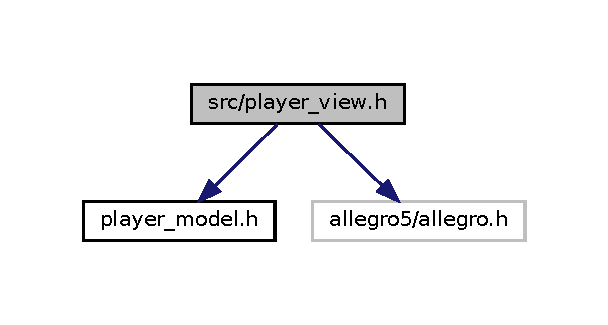
\includegraphics[width=292pt]{player__view_8h__incl}
\end{center}
\end{figure}
Граф файлов, в которые включается этот файл\+:\nopagebreak
\begin{figure}[H]
\begin{center}
\leavevmode
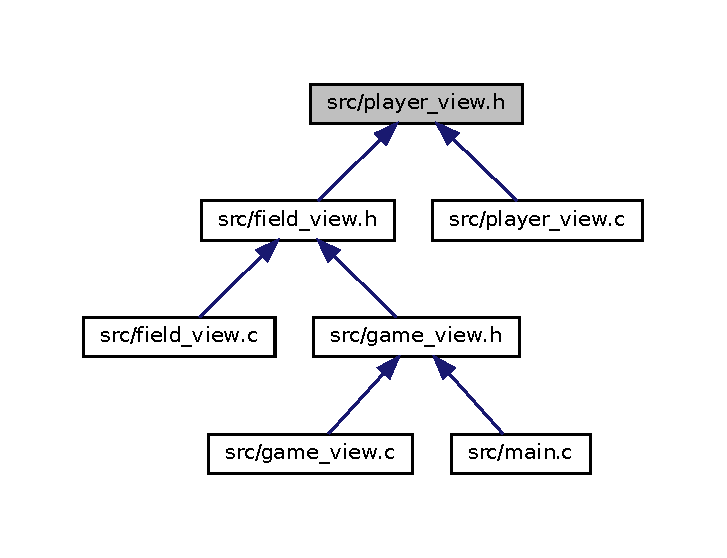
\includegraphics[width=349pt]{player__view_8h__dep__incl}
\end{center}
\end{figure}
\subsection*{Структуры данных}
\begin{DoxyCompactItemize}
\item 
struct \hyperlink{structplayer__view}{player\+\_\+view}
\begin{DoxyCompactList}\small\item\em Структура, которая описывает отображение игрока. \end{DoxyCompactList}\end{DoxyCompactItemize}
\subsection*{Макросы}
\begin{DoxyCompactItemize}
\item 
\#define \hyperlink{player__view_8h_a5fac8f2cc29ea5bde30c8fa4a4daa306}{P\+L\+A\+Y\+E\+R\+\_\+\+S\+I\+ZE}~50
\begin{DoxyCompactList}\small\item\em Размер игрока. \end{DoxyCompactList}\item 
\#define \hyperlink{player__view_8h_a28d88d882f8dc097928beffc901cc133}{P\+L\+A\+Y\+E\+R\+\_\+\+C\+O\+L\+OR}~al\+\_\+map\+\_\+rgb(30, 144, 255)
\begin{DoxyCompactList}\small\item\em Цвет игрока. \end{DoxyCompactList}\end{DoxyCompactItemize}
\subsection*{Определения типов}
\begin{DoxyCompactItemize}
\item 
typedef struct \hyperlink{structplayer__view}{player\+\_\+view} \hyperlink{player__view_8h_a2eb9f49a422f9ddd66caa41cd4033be8}{player\+\_\+view}
\end{DoxyCompactItemize}
\subsection*{Функции}
\begin{DoxyCompactItemize}
\item 
\hyperlink{structplayer__view}{player\+\_\+view} $\ast$ \hyperlink{player__view_8h_ad29d725f51acc28e6b284f0e124be650}{player\+\_\+view\+\_\+create} (\hyperlink{structplayer__model}{player\+\_\+model} $\ast$p\+\_\+model, unsigned int x\+\_\+start, unsigned int y\+\_\+start, unsigned int y\+\_\+finish)
\item 
int \hyperlink{player__view_8h_aabc16f780865d02b2f8a4f7719616cf1}{player\+\_\+view\+\_\+draw} (\hyperlink{structplayer__view}{player\+\_\+view} $\ast$p\+\_\+view)
\item 
int \hyperlink{player__view_8h_a8e15be2eea78a0500de34ac3773a1ed8}{player\+\_\+view\+\_\+destroy} (\hyperlink{structplayer__view}{player\+\_\+view} $\ast$p\+\_\+view)
\end{DoxyCompactItemize}


\subsection{Подробное описание}
Файл, в котором опеределены функции для работы с отображением игрока. 



\subsection{Макросы}
\mbox{\Hypertarget{player__view_8h_a28d88d882f8dc097928beffc901cc133}\label{player__view_8h_a28d88d882f8dc097928beffc901cc133}} 
\index{player\+\_\+view.\+h@{player\+\_\+view.\+h}!P\+L\+A\+Y\+E\+R\+\_\+\+C\+O\+L\+OR@{P\+L\+A\+Y\+E\+R\+\_\+\+C\+O\+L\+OR}}
\index{P\+L\+A\+Y\+E\+R\+\_\+\+C\+O\+L\+OR@{P\+L\+A\+Y\+E\+R\+\_\+\+C\+O\+L\+OR}!player\+\_\+view.\+h@{player\+\_\+view.\+h}}
\subsubsection{\texorpdfstring{P\+L\+A\+Y\+E\+R\+\_\+\+C\+O\+L\+OR}{PLAYER\_COLOR}}
{\footnotesize\ttfamily \#define P\+L\+A\+Y\+E\+R\+\_\+\+C\+O\+L\+OR~al\+\_\+map\+\_\+rgb(30, 144, 255)}



Цвет игрока. 

\mbox{\Hypertarget{player__view_8h_a5fac8f2cc29ea5bde30c8fa4a4daa306}\label{player__view_8h_a5fac8f2cc29ea5bde30c8fa4a4daa306}} 
\index{player\+\_\+view.\+h@{player\+\_\+view.\+h}!P\+L\+A\+Y\+E\+R\+\_\+\+S\+I\+ZE@{P\+L\+A\+Y\+E\+R\+\_\+\+S\+I\+ZE}}
\index{P\+L\+A\+Y\+E\+R\+\_\+\+S\+I\+ZE@{P\+L\+A\+Y\+E\+R\+\_\+\+S\+I\+ZE}!player\+\_\+view.\+h@{player\+\_\+view.\+h}}
\subsubsection{\texorpdfstring{P\+L\+A\+Y\+E\+R\+\_\+\+S\+I\+ZE}{PLAYER\_SIZE}}
{\footnotesize\ttfamily \#define P\+L\+A\+Y\+E\+R\+\_\+\+S\+I\+ZE~50}



Размер игрока. 



\subsection{Типы}
\mbox{\Hypertarget{player__view_8h_a2eb9f49a422f9ddd66caa41cd4033be8}\label{player__view_8h_a2eb9f49a422f9ddd66caa41cd4033be8}} 
\index{player\+\_\+view.\+h@{player\+\_\+view.\+h}!player\+\_\+view@{player\+\_\+view}}
\index{player\+\_\+view@{player\+\_\+view}!player\+\_\+view.\+h@{player\+\_\+view.\+h}}
\subsubsection{\texorpdfstring{player\+\_\+view}{player\_view}}
{\footnotesize\ttfamily typedef struct \hyperlink{structplayer__view}{player\+\_\+view} \hyperlink{structplayer__view}{player\+\_\+view}}



\subsection{Функции}
\mbox{\Hypertarget{player__view_8h_ad29d725f51acc28e6b284f0e124be650}\label{player__view_8h_ad29d725f51acc28e6b284f0e124be650}} 
\index{player\+\_\+view.\+h@{player\+\_\+view.\+h}!player\+\_\+view\+\_\+create@{player\+\_\+view\+\_\+create}}
\index{player\+\_\+view\+\_\+create@{player\+\_\+view\+\_\+create}!player\+\_\+view.\+h@{player\+\_\+view.\+h}}
\subsubsection{\texorpdfstring{player\+\_\+view\+\_\+create()}{player\_view\_create()}}
{\footnotesize\ttfamily \hyperlink{structplayer__view}{player\+\_\+view}$\ast$ player\+\_\+view\+\_\+create (\begin{DoxyParamCaption}\item[{\hyperlink{structplayer__model}{player\+\_\+model} $\ast$}]{p\+\_\+model,  }\item[{unsigned int}]{x\+\_\+start,  }\item[{unsigned int}]{y\+\_\+start,  }\item[{unsigned int}]{y\+\_\+finish }\end{DoxyParamCaption})}

Создание отображения игрока. 
\begin{DoxyParams}[1]{Аргументы}
\mbox{\tt in}  & {\em p\+\_\+model} & -\/ адрес модели игрока. \\
\hline
\mbox{\tt in}  & {\em x\+\_\+start} & -\/ координата верхнего левого угла начальной позиции игрока по оси OX. \\
\hline
\mbox{\tt in}  & {\em y\+\_\+start} & -\/ координата верхнего левого угла начальной позиции игрока по оси OY. \\
\hline
\mbox{\tt in}  & {\em y\+\_\+finish} & -\/ координата верхнего левого угла конечно позиции игрока по оси OY. \\
\hline
\end{DoxyParams}
\begin{DoxyReturn}{Возвращает}
Адрес, созданного отображения игрока. ~\newline
 N\+U\+LL, если во время создания отображения игрока произошла ошибка. 
\end{DoxyReturn}
\mbox{\Hypertarget{player__view_8h_a8e15be2eea78a0500de34ac3773a1ed8}\label{player__view_8h_a8e15be2eea78a0500de34ac3773a1ed8}} 
\index{player\+\_\+view.\+h@{player\+\_\+view.\+h}!player\+\_\+view\+\_\+destroy@{player\+\_\+view\+\_\+destroy}}
\index{player\+\_\+view\+\_\+destroy@{player\+\_\+view\+\_\+destroy}!player\+\_\+view.\+h@{player\+\_\+view.\+h}}
\subsubsection{\texorpdfstring{player\+\_\+view\+\_\+destroy()}{player\_view\_destroy()}}
{\footnotesize\ttfamily int player\+\_\+view\+\_\+destroy (\begin{DoxyParamCaption}\item[{\hyperlink{structplayer__view}{player\+\_\+view} $\ast$}]{p\+\_\+view }\end{DoxyParamCaption})}

Удаление отображения игрока. 
\begin{DoxyParams}[1]{Аргументы}
\mbox{\tt in}  & {\em p\+\_\+view} & -\/ адрес отображения игрока, которое нужно удалить. \\
\hline
\end{DoxyParams}
\begin{DoxyReturn}{Возвращает}
Ноль, если удаление прошло успешно. ~\newline
 Ненулевое число, если во время удаления произошла ошибка. 
\end{DoxyReturn}
\mbox{\Hypertarget{player__view_8h_aabc16f780865d02b2f8a4f7719616cf1}\label{player__view_8h_aabc16f780865d02b2f8a4f7719616cf1}} 
\index{player\+\_\+view.\+h@{player\+\_\+view.\+h}!player\+\_\+view\+\_\+draw@{player\+\_\+view\+\_\+draw}}
\index{player\+\_\+view\+\_\+draw@{player\+\_\+view\+\_\+draw}!player\+\_\+view.\+h@{player\+\_\+view.\+h}}
\subsubsection{\texorpdfstring{player\+\_\+view\+\_\+draw()}{player\_view\_draw()}}
{\footnotesize\ttfamily int player\+\_\+view\+\_\+draw (\begin{DoxyParamCaption}\item[{\hyperlink{structplayer__view}{player\+\_\+view} $\ast$}]{p\+\_\+view }\end{DoxyParamCaption})}

Рисование отображения игрока. 
\begin{DoxyParams}[1]{Аргументы}
\mbox{\tt in}  & {\em p\+\_\+view} & -\/ адрес отображения игрока, которое нужно нарисовать. \\
\hline
\end{DoxyParams}
\begin{DoxyReturn}{Возвращает}
Ноль, если отображение было успешно отрисовано. ~\newline
 Ненулевое число, если во время рисования произошла ошибка. 
\end{DoxyReturn}

\hypertarget{rectangle__view_8c}{}\section{Файл src/rectangle\+\_\+view.c}
\label{rectangle__view_8c}\index{src/rectangle\+\_\+view.\+c@{src/rectangle\+\_\+view.\+c}}


Файл, в котором реализованы функции для работы с элементом интерфейса\+: \char`\"{}прямоугольник\char`\"{}.  


{\ttfamily \#include \char`\"{}rectangle\+\_\+view.\+h\char`\"{}}\newline
{\ttfamily \#include \char`\"{}error\+\_\+report.\+h\char`\"{}}\newline
Граф включаемых заголовочных файлов для rectangle\+\_\+view.\+c\+:\nopagebreak
\begin{figure}[H]
\begin{center}
\leavevmode
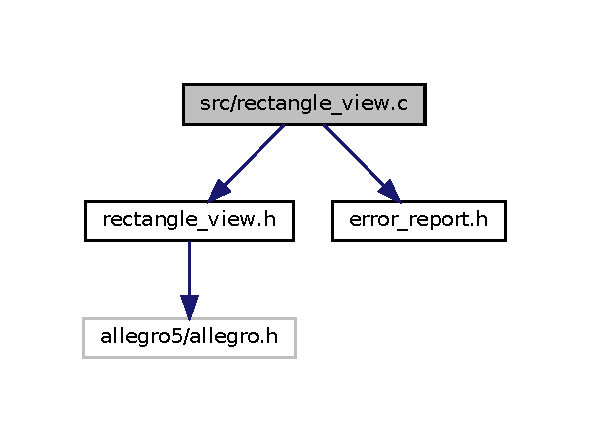
\includegraphics[width=283pt]{rectangle__view_8c__incl}
\end{center}
\end{figure}
\subsection*{Макросы}
\begin{DoxyCompactItemize}
\item 
\#define \hyperlink{rectangle__view_8c_ab117546549783a058d0321a287699579}{F\+I\+L\+E\+\_\+\+N\+A\+ME}~\char`\"{}rectangle\+\_\+view.\+c\char`\"{}
\begin{DoxyCompactList}\small\item\em Имя текущего файла. \end{DoxyCompactList}\item 
\#define \hyperlink{rectangle__view_8c_aba64ab31ac50908f7aa4125955fcf2ed}{F\+U\+N\+\_\+\+N\+A\+ME}~\char`\"{}rectangle\+\_\+view\+\_\+create\char`\"{}
\begin{DoxyCompactList}\small\item\em Имя текущей функции. \end{DoxyCompactList}\item 
\#define \hyperlink{rectangle__view_8c_aba64ab31ac50908f7aa4125955fcf2ed}{F\+U\+N\+\_\+\+N\+A\+ME}~\char`\"{}rectangle\+\_\+view\+\_\+draw\char`\"{}
\begin{DoxyCompactList}\small\item\em Имя текущей функции. \end{DoxyCompactList}\item 
\#define \hyperlink{rectangle__view_8c_aba64ab31ac50908f7aa4125955fcf2ed}{F\+U\+N\+\_\+\+N\+A\+ME}~\char`\"{}rectangle\+\_\+view\+\_\+destroy\char`\"{}
\begin{DoxyCompactList}\small\item\em Имя текущей функции. \end{DoxyCompactList}\end{DoxyCompactItemize}
\subsection*{Функции}
\begin{DoxyCompactItemize}
\item 
A\+L\+L\+E\+G\+R\+O\+\_\+\+B\+I\+T\+M\+AP $\ast$ \hyperlink{rectangle__view_8c_a31aa7ce2b4597a3b54945c36643c0e95}{rectangle\+\_\+view\+\_\+create} (A\+L\+L\+E\+G\+R\+O\+\_\+\+C\+O\+L\+OR color, unsigned int width, unsigned int height)
\item 
int \hyperlink{rectangle__view_8c_a5f254db4555257c9ed8562c4a2218539}{rectangle\+\_\+view\+\_\+draw} (A\+L\+L\+E\+G\+R\+O\+\_\+\+B\+I\+T\+M\+AP $\ast$r\+\_\+view, unsigned int x, unsigned int y)
\item 
int \hyperlink{rectangle__view_8c_a7cda47d97264b19f8529cac366da339f}{rectangle\+\_\+view\+\_\+destroy} (A\+L\+L\+E\+G\+R\+O\+\_\+\+B\+I\+T\+M\+AP $\ast$r\+\_\+view)
\end{DoxyCompactItemize}


\subsection{Подробное описание}
Файл, в котором реализованы функции для работы с элементом интерфейса\+: \char`\"{}прямоугольник\char`\"{}. 



\subsection{Макросы}
\mbox{\Hypertarget{rectangle__view_8c_ab117546549783a058d0321a287699579}\label{rectangle__view_8c_ab117546549783a058d0321a287699579}} 
\index{rectangle\+\_\+view.\+c@{rectangle\+\_\+view.\+c}!F\+I\+L\+E\+\_\+\+N\+A\+ME@{F\+I\+L\+E\+\_\+\+N\+A\+ME}}
\index{F\+I\+L\+E\+\_\+\+N\+A\+ME@{F\+I\+L\+E\+\_\+\+N\+A\+ME}!rectangle\+\_\+view.\+c@{rectangle\+\_\+view.\+c}}
\subsubsection{\texorpdfstring{F\+I\+L\+E\+\_\+\+N\+A\+ME}{FILE\_NAME}}
{\footnotesize\ttfamily \#define F\+I\+L\+E\+\_\+\+N\+A\+ME~\char`\"{}rectangle\+\_\+view.\+c\char`\"{}}



Имя текущего файла. 

\mbox{\Hypertarget{rectangle__view_8c_aba64ab31ac50908f7aa4125955fcf2ed}\label{rectangle__view_8c_aba64ab31ac50908f7aa4125955fcf2ed}} 
\index{rectangle\+\_\+view.\+c@{rectangle\+\_\+view.\+c}!F\+U\+N\+\_\+\+N\+A\+ME@{F\+U\+N\+\_\+\+N\+A\+ME}}
\index{F\+U\+N\+\_\+\+N\+A\+ME@{F\+U\+N\+\_\+\+N\+A\+ME}!rectangle\+\_\+view.\+c@{rectangle\+\_\+view.\+c}}
\subsubsection{\texorpdfstring{F\+U\+N\+\_\+\+N\+A\+ME}{FUN\_NAME}\hspace{0.1cm}{\footnotesize\ttfamily [1/3]}}
{\footnotesize\ttfamily \#define F\+U\+N\+\_\+\+N\+A\+ME~\char`\"{}rectangle\+\_\+view\+\_\+create\char`\"{}}



Имя текущей функции. 

\mbox{\Hypertarget{rectangle__view_8c_aba64ab31ac50908f7aa4125955fcf2ed}\label{rectangle__view_8c_aba64ab31ac50908f7aa4125955fcf2ed}} 
\index{rectangle\+\_\+view.\+c@{rectangle\+\_\+view.\+c}!F\+U\+N\+\_\+\+N\+A\+ME@{F\+U\+N\+\_\+\+N\+A\+ME}}
\index{F\+U\+N\+\_\+\+N\+A\+ME@{F\+U\+N\+\_\+\+N\+A\+ME}!rectangle\+\_\+view.\+c@{rectangle\+\_\+view.\+c}}
\subsubsection{\texorpdfstring{F\+U\+N\+\_\+\+N\+A\+ME}{FUN\_NAME}\hspace{0.1cm}{\footnotesize\ttfamily [2/3]}}
{\footnotesize\ttfamily \#define F\+U\+N\+\_\+\+N\+A\+ME~\char`\"{}rectangle\+\_\+view\+\_\+draw\char`\"{}}



Имя текущей функции. 

\mbox{\Hypertarget{rectangle__view_8c_aba64ab31ac50908f7aa4125955fcf2ed}\label{rectangle__view_8c_aba64ab31ac50908f7aa4125955fcf2ed}} 
\index{rectangle\+\_\+view.\+c@{rectangle\+\_\+view.\+c}!F\+U\+N\+\_\+\+N\+A\+ME@{F\+U\+N\+\_\+\+N\+A\+ME}}
\index{F\+U\+N\+\_\+\+N\+A\+ME@{F\+U\+N\+\_\+\+N\+A\+ME}!rectangle\+\_\+view.\+c@{rectangle\+\_\+view.\+c}}
\subsubsection{\texorpdfstring{F\+U\+N\+\_\+\+N\+A\+ME}{FUN\_NAME}\hspace{0.1cm}{\footnotesize\ttfamily [3/3]}}
{\footnotesize\ttfamily \#define F\+U\+N\+\_\+\+N\+A\+ME~\char`\"{}rectangle\+\_\+view\+\_\+destroy\char`\"{}}



Имя текущей функции. 



\subsection{Функции}
\mbox{\Hypertarget{rectangle__view_8c_a31aa7ce2b4597a3b54945c36643c0e95}\label{rectangle__view_8c_a31aa7ce2b4597a3b54945c36643c0e95}} 
\index{rectangle\+\_\+view.\+c@{rectangle\+\_\+view.\+c}!rectangle\+\_\+view\+\_\+create@{rectangle\+\_\+view\+\_\+create}}
\index{rectangle\+\_\+view\+\_\+create@{rectangle\+\_\+view\+\_\+create}!rectangle\+\_\+view.\+c@{rectangle\+\_\+view.\+c}}
\subsubsection{\texorpdfstring{rectangle\+\_\+view\+\_\+create()}{rectangle\_view\_create()}}
{\footnotesize\ttfamily A\+L\+L\+E\+G\+R\+O\+\_\+\+B\+I\+T\+M\+AP$\ast$ rectangle\+\_\+view\+\_\+create (\begin{DoxyParamCaption}\item[{A\+L\+L\+E\+G\+R\+O\+\_\+\+C\+O\+L\+OR}]{color,  }\item[{unsigned int}]{width,  }\item[{unsigned int}]{height }\end{DoxyParamCaption})}

Создание прямоугольника. 
\begin{DoxyParams}[1]{Аргументы}
\mbox{\tt in}  & {\em color} & -\/ цвет. \\
\hline
\mbox{\tt in}  & {\em width} & -\/ ширина. \\
\hline
\mbox{\tt in}  & {\em height} & -\/ высота. \\
\hline
\end{DoxyParams}
\begin{DoxyReturn}{Возвращает}
Адрес, созданного прямоугольника. ~\newline
 N\+U\+LL, если во время создания прямоугольника произошла ошибка. 
\end{DoxyReturn}
\mbox{\Hypertarget{rectangle__view_8c_a7cda47d97264b19f8529cac366da339f}\label{rectangle__view_8c_a7cda47d97264b19f8529cac366da339f}} 
\index{rectangle\+\_\+view.\+c@{rectangle\+\_\+view.\+c}!rectangle\+\_\+view\+\_\+destroy@{rectangle\+\_\+view\+\_\+destroy}}
\index{rectangle\+\_\+view\+\_\+destroy@{rectangle\+\_\+view\+\_\+destroy}!rectangle\+\_\+view.\+c@{rectangle\+\_\+view.\+c}}
\subsubsection{\texorpdfstring{rectangle\+\_\+view\+\_\+destroy()}{rectangle\_view\_destroy()}}
{\footnotesize\ttfamily int rectangle\+\_\+view\+\_\+destroy (\begin{DoxyParamCaption}\item[{A\+L\+L\+E\+G\+R\+O\+\_\+\+B\+I\+T\+M\+AP $\ast$}]{r\+\_\+view }\end{DoxyParamCaption})}

Удаление прямоугольника. 
\begin{DoxyParams}[1]{Аргументы}
\mbox{\tt in}  & {\em r\+\_\+view} & -\/ адрес прямоугольника, который нужно удалить. \\
\hline
\end{DoxyParams}
\begin{DoxyReturn}{Возвращает}
Ноль, если удаление прошло успешно. ~\newline
 Ненулевое число, если во время удаления произошла ошибка. 
\end{DoxyReturn}
\mbox{\Hypertarget{rectangle__view_8c_a5f254db4555257c9ed8562c4a2218539}\label{rectangle__view_8c_a5f254db4555257c9ed8562c4a2218539}} 
\index{rectangle\+\_\+view.\+c@{rectangle\+\_\+view.\+c}!rectangle\+\_\+view\+\_\+draw@{rectangle\+\_\+view\+\_\+draw}}
\index{rectangle\+\_\+view\+\_\+draw@{rectangle\+\_\+view\+\_\+draw}!rectangle\+\_\+view.\+c@{rectangle\+\_\+view.\+c}}
\subsubsection{\texorpdfstring{rectangle\+\_\+view\+\_\+draw()}{rectangle\_view\_draw()}}
{\footnotesize\ttfamily int rectangle\+\_\+view\+\_\+draw (\begin{DoxyParamCaption}\item[{A\+L\+L\+E\+G\+R\+O\+\_\+\+B\+I\+T\+M\+AP $\ast$}]{r\+\_\+view,  }\item[{unsigned int}]{x,  }\item[{unsigned int}]{y }\end{DoxyParamCaption})}

Рисование треугольника. 
\begin{DoxyParams}[1]{Аргументы}
\mbox{\tt in}  & {\em r\+\_\+view} & -\/ адрес прямоугольника, который нужно нарисовать. \\
\hline
\mbox{\tt in}  & {\em x} & -\/ координата рисования верхнего левого угла прямоугольника по оси OX. \\
\hline
\mbox{\tt in}  & {\em y} & -\/ координата рисования верхнего левого угла прямоугольника по оси OY. \\
\hline
\end{DoxyParams}
\begin{DoxyReturn}{Возвращает}
Ноль, если прямоугольник был успешно отрисован. ~\newline
 Ненулевое число, если во время рисования произошла ошибка. 
\end{DoxyReturn}

\hypertarget{rectangle__view_8h}{}\section{Файл src/rectangle\+\_\+view.h}
\label{rectangle__view_8h}\index{src/rectangle\+\_\+view.\+h@{src/rectangle\+\_\+view.\+h}}


Файл, в котором опеределены функции для работы с элементом интерфейса\+: \char`\"{}прямоугольник\char`\"{}.  


{\ttfamily \#include $<$allegro5/allegro.\+h$>$}\newline
Граф включаемых заголовочных файлов для rectangle\+\_\+view.\+h\+:\nopagebreak
\begin{figure}[H]
\begin{center}
\leavevmode
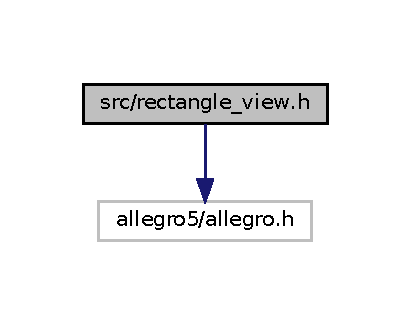
\includegraphics[width=197pt]{rectangle__view_8h__incl}
\end{center}
\end{figure}
Граф файлов, в которые включается этот файл\+:\nopagebreak
\begin{figure}[H]
\begin{center}
\leavevmode
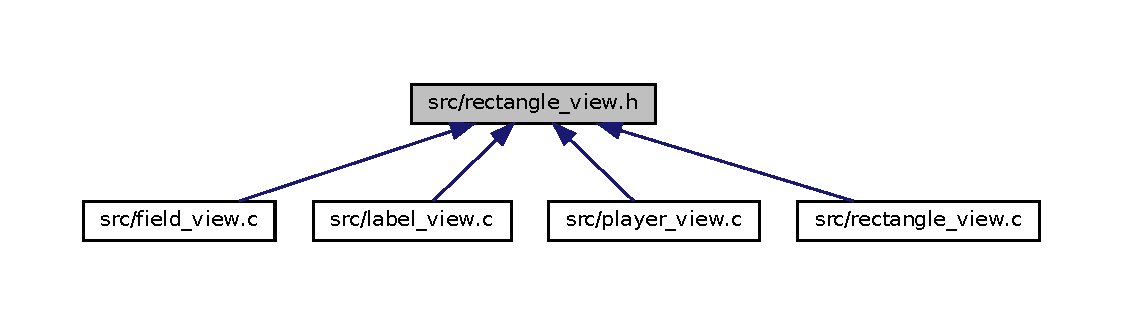
\includegraphics[width=350pt]{rectangle__view_8h__dep__incl}
\end{center}
\end{figure}
\subsection*{Функции}
\begin{DoxyCompactItemize}
\item 
A\+L\+L\+E\+G\+R\+O\+\_\+\+B\+I\+T\+M\+AP $\ast$ \hyperlink{rectangle__view_8h_a31aa7ce2b4597a3b54945c36643c0e95}{rectangle\+\_\+view\+\_\+create} (A\+L\+L\+E\+G\+R\+O\+\_\+\+C\+O\+L\+OR color, unsigned int width, unsigned int height)
\item 
int \hyperlink{rectangle__view_8h_a5f254db4555257c9ed8562c4a2218539}{rectangle\+\_\+view\+\_\+draw} (A\+L\+L\+E\+G\+R\+O\+\_\+\+B\+I\+T\+M\+AP $\ast$r\+\_\+view, unsigned int x, unsigned int y)
\item 
int \hyperlink{rectangle__view_8h_a7cda47d97264b19f8529cac366da339f}{rectangle\+\_\+view\+\_\+destroy} (A\+L\+L\+E\+G\+R\+O\+\_\+\+B\+I\+T\+M\+AP $\ast$r\+\_\+view)
\end{DoxyCompactItemize}


\subsection{Подробное описание}
Файл, в котором опеределены функции для работы с элементом интерфейса\+: \char`\"{}прямоугольник\char`\"{}. 



\subsection{Функции}
\mbox{\Hypertarget{rectangle__view_8h_a31aa7ce2b4597a3b54945c36643c0e95}\label{rectangle__view_8h_a31aa7ce2b4597a3b54945c36643c0e95}} 
\index{rectangle\+\_\+view.\+h@{rectangle\+\_\+view.\+h}!rectangle\+\_\+view\+\_\+create@{rectangle\+\_\+view\+\_\+create}}
\index{rectangle\+\_\+view\+\_\+create@{rectangle\+\_\+view\+\_\+create}!rectangle\+\_\+view.\+h@{rectangle\+\_\+view.\+h}}
\subsubsection{\texorpdfstring{rectangle\+\_\+view\+\_\+create()}{rectangle\_view\_create()}}
{\footnotesize\ttfamily A\+L\+L\+E\+G\+R\+O\+\_\+\+B\+I\+T\+M\+AP$\ast$ rectangle\+\_\+view\+\_\+create (\begin{DoxyParamCaption}\item[{A\+L\+L\+E\+G\+R\+O\+\_\+\+C\+O\+L\+OR}]{color,  }\item[{unsigned int}]{width,  }\item[{unsigned int}]{height }\end{DoxyParamCaption})}

Создание прямоугольника. 
\begin{DoxyParams}[1]{Аргументы}
\mbox{\tt in}  & {\em color} & -\/ цвет. \\
\hline
\mbox{\tt in}  & {\em width} & -\/ ширина. \\
\hline
\mbox{\tt in}  & {\em height} & -\/ высота. \\
\hline
\end{DoxyParams}
\begin{DoxyReturn}{Возвращает}
Адрес, созданного прямоугольника. ~\newline
 N\+U\+LL, если во время создания прямоугольника произошла ошибка. 
\end{DoxyReturn}
\mbox{\Hypertarget{rectangle__view_8h_a7cda47d97264b19f8529cac366da339f}\label{rectangle__view_8h_a7cda47d97264b19f8529cac366da339f}} 
\index{rectangle\+\_\+view.\+h@{rectangle\+\_\+view.\+h}!rectangle\+\_\+view\+\_\+destroy@{rectangle\+\_\+view\+\_\+destroy}}
\index{rectangle\+\_\+view\+\_\+destroy@{rectangle\+\_\+view\+\_\+destroy}!rectangle\+\_\+view.\+h@{rectangle\+\_\+view.\+h}}
\subsubsection{\texorpdfstring{rectangle\+\_\+view\+\_\+destroy()}{rectangle\_view\_destroy()}}
{\footnotesize\ttfamily int rectangle\+\_\+view\+\_\+destroy (\begin{DoxyParamCaption}\item[{A\+L\+L\+E\+G\+R\+O\+\_\+\+B\+I\+T\+M\+AP $\ast$}]{r\+\_\+view }\end{DoxyParamCaption})}

Удаление прямоугольника. 
\begin{DoxyParams}[1]{Аргументы}
\mbox{\tt in}  & {\em r\+\_\+view} & -\/ адрес прямоугольника, который нужно удалить. \\
\hline
\end{DoxyParams}
\begin{DoxyReturn}{Возвращает}
Ноль, если удаление прошло успешно. ~\newline
 Ненулевое число, если во время удаления произошла ошибка. 
\end{DoxyReturn}
\mbox{\Hypertarget{rectangle__view_8h_a5f254db4555257c9ed8562c4a2218539}\label{rectangle__view_8h_a5f254db4555257c9ed8562c4a2218539}} 
\index{rectangle\+\_\+view.\+h@{rectangle\+\_\+view.\+h}!rectangle\+\_\+view\+\_\+draw@{rectangle\+\_\+view\+\_\+draw}}
\index{rectangle\+\_\+view\+\_\+draw@{rectangle\+\_\+view\+\_\+draw}!rectangle\+\_\+view.\+h@{rectangle\+\_\+view.\+h}}
\subsubsection{\texorpdfstring{rectangle\+\_\+view\+\_\+draw()}{rectangle\_view\_draw()}}
{\footnotesize\ttfamily int rectangle\+\_\+view\+\_\+draw (\begin{DoxyParamCaption}\item[{A\+L\+L\+E\+G\+R\+O\+\_\+\+B\+I\+T\+M\+AP $\ast$}]{r\+\_\+view,  }\item[{unsigned int}]{x,  }\item[{unsigned int}]{y }\end{DoxyParamCaption})}

Рисование треугольника. 
\begin{DoxyParams}[1]{Аргументы}
\mbox{\tt in}  & {\em r\+\_\+view} & -\/ адрес прямоугольника, который нужно нарисовать. \\
\hline
\mbox{\tt in}  & {\em x} & -\/ координата рисования верхнего левого угла прямоугольника по оси OX. \\
\hline
\mbox{\tt in}  & {\em y} & -\/ координата рисования верхнего левого угла прямоугольника по оси OY. \\
\hline
\end{DoxyParams}
\begin{DoxyReturn}{Возвращает}
Ноль, если прямоугольник был успешно отрисован. ~\newline
 Ненулевое число, если во время рисования произошла ошибка. 
\end{DoxyReturn}

\hypertarget{runner_8c}{}\section{Файл src/test/runner.c}
\label{runner_8c}\index{src/test/runner.\+c@{src/test/runner.\+c}}


Функция запуска всех тестов.  


{\ttfamily \#include \char`\"{}unity.\+h\char`\"{}}\newline
{\ttfamily \#include \char`\"{}unity\+\_\+fixture.\+h\char`\"{}}\newline
Граф включаемых заголовочных файлов для runner.\+c\+:\nopagebreak
\begin{figure}[H]
\begin{center}
\leavevmode
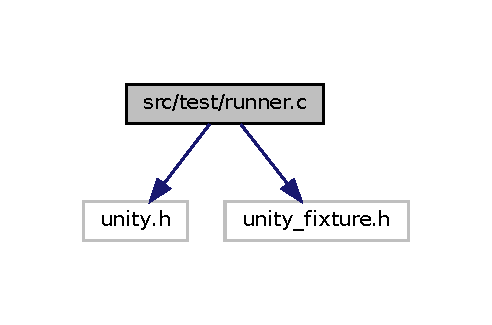
\includegraphics[width=236pt]{runner_8c__incl}
\end{center}
\end{figure}
\subsection*{Функции}
\begin{DoxyCompactItemize}
\item 
int \hyperlink{runner_8c_ac0f2228420376f4db7e1274f2b41667c}{main} (int argc, const char $\ast$argv\mbox{[}$\,$\mbox{]})
\end{DoxyCompactItemize}


\subsection{Подробное описание}
Функция запуска всех тестов. 



\subsection{Функции}
\mbox{\Hypertarget{runner_8c_ac0f2228420376f4db7e1274f2b41667c}\label{runner_8c_ac0f2228420376f4db7e1274f2b41667c}} 
\index{runner.\+c@{runner.\+c}!main@{main}}
\index{main@{main}!runner.\+c@{runner.\+c}}
\subsubsection{\texorpdfstring{main()}{main()}}
{\footnotesize\ttfamily int main (\begin{DoxyParamCaption}\item[{int}]{argc,  }\item[{const char $\ast$}]{argv\mbox{[}$\,$\mbox{]} }\end{DoxyParamCaption})}


\hypertarget{test___game_model_8c}{}\section{Файл src/test/test\+\_\+\+Game\+Model.c}
\label{test___game_model_8c}\index{src/test/test\+\_\+\+Game\+Model.\+c@{src/test/test\+\_\+\+Game\+Model.\+c}}


Файл тестирующий игровую модель.  


{\ttfamily \#include \char`\"{}unity.\+h\char`\"{}}\newline
{\ttfamily \#include \char`\"{}unity\+\_\+fixture.\+h\char`\"{}}\newline
{\ttfamily \#include \char`\"{}game\+\_\+model.\+h\char`\"{}}\newline
{\ttfamily \#include $<$stdlib.\+h$>$}\newline
Граф включаемых заголовочных файлов для test\+\_\+\+Game\+Model.\+c\+:\nopagebreak
\begin{figure}[H]
\begin{center}
\leavevmode
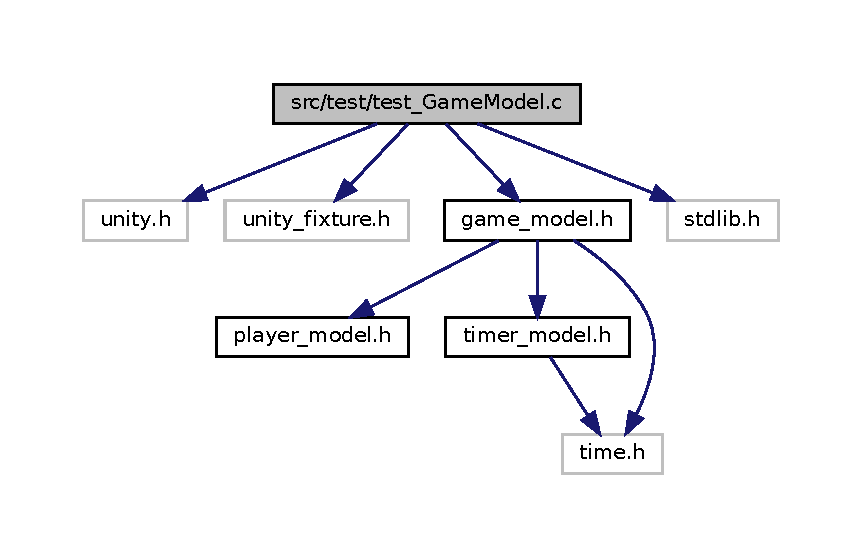
\includegraphics[width=350pt]{test___game_model_8c__incl}
\end{center}
\end{figure}
\subsection*{Функции}
\begin{DoxyCompactItemize}
\item 
\hyperlink{test___game_model_8c_a66ab246bd3e1b561c51303f68beab387}{T\+E\+S\+T\+\_\+\+G\+R\+O\+UP} (Test\+Game\+Model)
\item 
\hyperlink{test___game_model_8c_a89456d952119016de84cad6aaeae5d3a}{T\+E\+S\+T\+\_\+\+G\+R\+O\+U\+P\+\_\+\+R\+U\+N\+N\+ER} (Test\+Game\+Model)
\item 
\hyperlink{test___game_model_8c_a844ef9378bfe7eef9159770c9f9feb31}{T\+E\+S\+T\+\_\+\+S\+E\+T\+UP} (Test\+Game\+Model)
\item 
\hyperlink{test___game_model_8c_ac1153ea1095cca39509ec02e4648fc5b}{T\+E\+S\+T\+\_\+\+T\+E\+A\+R\+\_\+\+D\+O\+WN} (Test\+Game\+Model)
\item 
\hyperlink{test___game_model_8c_a6e2ad3fe1dbe35631faf0f709494b913}{T\+E\+ST} (Test\+Game\+Model, Function\+Create)
\item 
\hyperlink{test___game_model_8c_aeb7eceb745521f1b15e3c408d09482b9}{T\+E\+ST} (Test\+Game\+Model, Function\+Destroy)
\item 
\hyperlink{test___game_model_8c_a0c847b6a0c8476b3fad60a5a3d272017}{T\+E\+ST} (Test\+Game\+Model, Function\+Is\+End)
\item 
\hyperlink{test___game_model_8c_a4d3dce20e427824085f9760e4b4557e0}{T\+E\+ST} (Test\+Game\+Model, Function\+Key\+Down)
\item 
\hyperlink{test___game_model_8c_a59e67813db998fa1b832b5053617224f}{T\+E\+ST} (Test\+Game\+Model, Function\+Start)
\item 
\hyperlink{test___game_model_8c_a528d0add3ebe74f17da7013d382c3a8d}{T\+E\+ST} (Test\+Game\+Model, Function\+Update)
\end{DoxyCompactItemize}


\subsection{Подробное описание}
Файл тестирующий игровую модель. 



\subsection{Функции}
\mbox{\Hypertarget{test___game_model_8c_a6e2ad3fe1dbe35631faf0f709494b913}\label{test___game_model_8c_a6e2ad3fe1dbe35631faf0f709494b913}} 
\index{test\+\_\+\+Game\+Model.\+c@{test\+\_\+\+Game\+Model.\+c}!T\+E\+ST@{T\+E\+ST}}
\index{T\+E\+ST@{T\+E\+ST}!test\+\_\+\+Game\+Model.\+c@{test\+\_\+\+Game\+Model.\+c}}
\subsubsection{\texorpdfstring{T\+E\+S\+T()}{TEST()}\hspace{0.1cm}{\footnotesize\ttfamily [1/6]}}
{\footnotesize\ttfamily T\+E\+ST (\begin{DoxyParamCaption}\item[{Test\+Game\+Model}]{,  }\item[{Function\+Create}]{ }\end{DoxyParamCaption})}

Функция, которая тестирует функцию game\+\_\+model\+\_\+create. \mbox{\Hypertarget{test___game_model_8c_aeb7eceb745521f1b15e3c408d09482b9}\label{test___game_model_8c_aeb7eceb745521f1b15e3c408d09482b9}} 
\index{test\+\_\+\+Game\+Model.\+c@{test\+\_\+\+Game\+Model.\+c}!T\+E\+ST@{T\+E\+ST}}
\index{T\+E\+ST@{T\+E\+ST}!test\+\_\+\+Game\+Model.\+c@{test\+\_\+\+Game\+Model.\+c}}
\subsubsection{\texorpdfstring{T\+E\+S\+T()}{TEST()}\hspace{0.1cm}{\footnotesize\ttfamily [2/6]}}
{\footnotesize\ttfamily T\+E\+ST (\begin{DoxyParamCaption}\item[{Test\+Game\+Model}]{,  }\item[{Function\+Destroy}]{ }\end{DoxyParamCaption})}

Функция, которая тестирует функцию game\+\_\+model\+\_\+destroy. \mbox{\Hypertarget{test___game_model_8c_a0c847b6a0c8476b3fad60a5a3d272017}\label{test___game_model_8c_a0c847b6a0c8476b3fad60a5a3d272017}} 
\index{test\+\_\+\+Game\+Model.\+c@{test\+\_\+\+Game\+Model.\+c}!T\+E\+ST@{T\+E\+ST}}
\index{T\+E\+ST@{T\+E\+ST}!test\+\_\+\+Game\+Model.\+c@{test\+\_\+\+Game\+Model.\+c}}
\subsubsection{\texorpdfstring{T\+E\+S\+T()}{TEST()}\hspace{0.1cm}{\footnotesize\ttfamily [3/6]}}
{\footnotesize\ttfamily T\+E\+ST (\begin{DoxyParamCaption}\item[{Test\+Game\+Model}]{,  }\item[{Function\+Is\+End}]{ }\end{DoxyParamCaption})}

Функция, которая тестирует функцию game\+\_\+model\+\_\+is\+\_\+end. \mbox{\Hypertarget{test___game_model_8c_a4d3dce20e427824085f9760e4b4557e0}\label{test___game_model_8c_a4d3dce20e427824085f9760e4b4557e0}} 
\index{test\+\_\+\+Game\+Model.\+c@{test\+\_\+\+Game\+Model.\+c}!T\+E\+ST@{T\+E\+ST}}
\index{T\+E\+ST@{T\+E\+ST}!test\+\_\+\+Game\+Model.\+c@{test\+\_\+\+Game\+Model.\+c}}
\subsubsection{\texorpdfstring{T\+E\+S\+T()}{TEST()}\hspace{0.1cm}{\footnotesize\ttfamily [4/6]}}
{\footnotesize\ttfamily T\+E\+ST (\begin{DoxyParamCaption}\item[{Test\+Game\+Model}]{,  }\item[{Function\+Key\+Down}]{ }\end{DoxyParamCaption})}

Функция, которая тестирует функцию game\+\_\+model\+\_\+key\+\_\+down. \mbox{\Hypertarget{test___game_model_8c_a59e67813db998fa1b832b5053617224f}\label{test___game_model_8c_a59e67813db998fa1b832b5053617224f}} 
\index{test\+\_\+\+Game\+Model.\+c@{test\+\_\+\+Game\+Model.\+c}!T\+E\+ST@{T\+E\+ST}}
\index{T\+E\+ST@{T\+E\+ST}!test\+\_\+\+Game\+Model.\+c@{test\+\_\+\+Game\+Model.\+c}}
\subsubsection{\texorpdfstring{T\+E\+S\+T()}{TEST()}\hspace{0.1cm}{\footnotesize\ttfamily [5/6]}}
{\footnotesize\ttfamily T\+E\+ST (\begin{DoxyParamCaption}\item[{Test\+Game\+Model}]{,  }\item[{Function\+Start}]{ }\end{DoxyParamCaption})}

Функция, которая тестирует функцию game\+\_\+model\+\_\+start. \mbox{\Hypertarget{test___game_model_8c_a528d0add3ebe74f17da7013d382c3a8d}\label{test___game_model_8c_a528d0add3ebe74f17da7013d382c3a8d}} 
\index{test\+\_\+\+Game\+Model.\+c@{test\+\_\+\+Game\+Model.\+c}!T\+E\+ST@{T\+E\+ST}}
\index{T\+E\+ST@{T\+E\+ST}!test\+\_\+\+Game\+Model.\+c@{test\+\_\+\+Game\+Model.\+c}}
\subsubsection{\texorpdfstring{T\+E\+S\+T()}{TEST()}\hspace{0.1cm}{\footnotesize\ttfamily [6/6]}}
{\footnotesize\ttfamily T\+E\+ST (\begin{DoxyParamCaption}\item[{Test\+Game\+Model}]{,  }\item[{Function\+Update}]{ }\end{DoxyParamCaption})}

Функция, которая тестирует функцию game\+\_\+model\+\_\+update. \mbox{\Hypertarget{test___game_model_8c_a66ab246bd3e1b561c51303f68beab387}\label{test___game_model_8c_a66ab246bd3e1b561c51303f68beab387}} 
\index{test\+\_\+\+Game\+Model.\+c@{test\+\_\+\+Game\+Model.\+c}!T\+E\+S\+T\+\_\+\+G\+R\+O\+UP@{T\+E\+S\+T\+\_\+\+G\+R\+O\+UP}}
\index{T\+E\+S\+T\+\_\+\+G\+R\+O\+UP@{T\+E\+S\+T\+\_\+\+G\+R\+O\+UP}!test\+\_\+\+Game\+Model.\+c@{test\+\_\+\+Game\+Model.\+c}}
\subsubsection{\texorpdfstring{T\+E\+S\+T\+\_\+\+G\+R\+O\+U\+P()}{TEST\_GROUP()}}
{\footnotesize\ttfamily T\+E\+S\+T\+\_\+\+G\+R\+O\+UP (\begin{DoxyParamCaption}\item[{Test\+Game\+Model}]{ }\end{DoxyParamCaption})}

\mbox{\Hypertarget{test___game_model_8c_a89456d952119016de84cad6aaeae5d3a}\label{test___game_model_8c_a89456d952119016de84cad6aaeae5d3a}} 
\index{test\+\_\+\+Game\+Model.\+c@{test\+\_\+\+Game\+Model.\+c}!T\+E\+S\+T\+\_\+\+G\+R\+O\+U\+P\+\_\+\+R\+U\+N\+N\+ER@{T\+E\+S\+T\+\_\+\+G\+R\+O\+U\+P\+\_\+\+R\+U\+N\+N\+ER}}
\index{T\+E\+S\+T\+\_\+\+G\+R\+O\+U\+P\+\_\+\+R\+U\+N\+N\+ER@{T\+E\+S\+T\+\_\+\+G\+R\+O\+U\+P\+\_\+\+R\+U\+N\+N\+ER}!test\+\_\+\+Game\+Model.\+c@{test\+\_\+\+Game\+Model.\+c}}
\subsubsection{\texorpdfstring{T\+E\+S\+T\+\_\+\+G\+R\+O\+U\+P\+\_\+\+R\+U\+N\+N\+E\+R()}{TEST\_GROUP\_RUNNER()}}
{\footnotesize\ttfamily T\+E\+S\+T\+\_\+\+G\+R\+O\+U\+P\+\_\+\+R\+U\+N\+N\+ER (\begin{DoxyParamCaption}\item[{Test\+Game\+Model}]{ }\end{DoxyParamCaption})}

\mbox{\Hypertarget{test___game_model_8c_a844ef9378bfe7eef9159770c9f9feb31}\label{test___game_model_8c_a844ef9378bfe7eef9159770c9f9feb31}} 
\index{test\+\_\+\+Game\+Model.\+c@{test\+\_\+\+Game\+Model.\+c}!T\+E\+S\+T\+\_\+\+S\+E\+T\+UP@{T\+E\+S\+T\+\_\+\+S\+E\+T\+UP}}
\index{T\+E\+S\+T\+\_\+\+S\+E\+T\+UP@{T\+E\+S\+T\+\_\+\+S\+E\+T\+UP}!test\+\_\+\+Game\+Model.\+c@{test\+\_\+\+Game\+Model.\+c}}
\subsubsection{\texorpdfstring{T\+E\+S\+T\+\_\+\+S\+E\+T\+U\+P()}{TEST\_SETUP()}}
{\footnotesize\ttfamily T\+E\+S\+T\+\_\+\+S\+E\+T\+UP (\begin{DoxyParamCaption}\item[{Test\+Game\+Model}]{ }\end{DoxyParamCaption})}

\mbox{\Hypertarget{test___game_model_8c_ac1153ea1095cca39509ec02e4648fc5b}\label{test___game_model_8c_ac1153ea1095cca39509ec02e4648fc5b}} 
\index{test\+\_\+\+Game\+Model.\+c@{test\+\_\+\+Game\+Model.\+c}!T\+E\+S\+T\+\_\+\+T\+E\+A\+R\+\_\+\+D\+O\+WN@{T\+E\+S\+T\+\_\+\+T\+E\+A\+R\+\_\+\+D\+O\+WN}}
\index{T\+E\+S\+T\+\_\+\+T\+E\+A\+R\+\_\+\+D\+O\+WN@{T\+E\+S\+T\+\_\+\+T\+E\+A\+R\+\_\+\+D\+O\+WN}!test\+\_\+\+Game\+Model.\+c@{test\+\_\+\+Game\+Model.\+c}}
\subsubsection{\texorpdfstring{T\+E\+S\+T\+\_\+\+T\+E\+A\+R\+\_\+\+D\+O\+W\+N()}{TEST\_TEAR\_DOWN()}}
{\footnotesize\ttfamily T\+E\+S\+T\+\_\+\+T\+E\+A\+R\+\_\+\+D\+O\+WN (\begin{DoxyParamCaption}\item[{Test\+Game\+Model}]{ }\end{DoxyParamCaption})}


\hypertarget{test___player_model_8c}{}\section{Файл src/test/test\+\_\+\+Player\+Model.c}
\label{test___player_model_8c}\index{src/test/test\+\_\+\+Player\+Model.\+c@{src/test/test\+\_\+\+Player\+Model.\+c}}


Файл тестирующий модель игрока.  


{\ttfamily \#include \char`\"{}unity.\+h\char`\"{}}\newline
{\ttfamily \#include \char`\"{}unity\+\_\+fixture.\+h\char`\"{}}\newline
{\ttfamily \#include \char`\"{}player\+\_\+model.\+h\char`\"{}}\newline
{\ttfamily \#include $<$stdlib.\+h$>$}\newline
Граф включаемых заголовочных файлов для test\+\_\+\+Player\+Model.\+c\+:\nopagebreak
\begin{figure}[H]
\begin{center}
\leavevmode
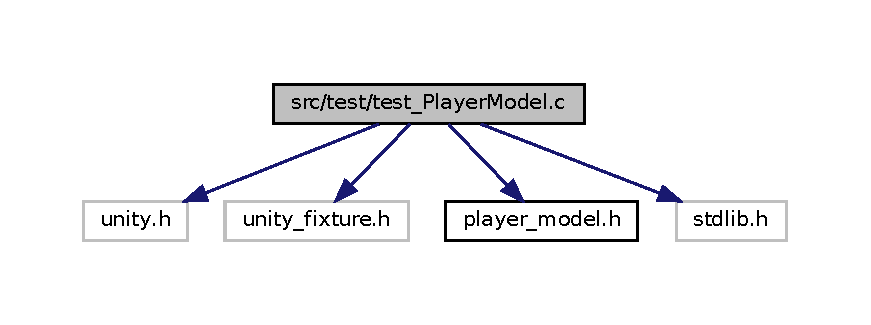
\includegraphics[width=350pt]{test___player_model_8c__incl}
\end{center}
\end{figure}
\subsection*{Функции}
\begin{DoxyCompactItemize}
\item 
\hyperlink{test___player_model_8c_a163cd6e6a9cda4077f25ccfb162d2760}{T\+E\+S\+T\+\_\+\+G\+R\+O\+UP} (Test\+Player\+Model)
\item 
\hyperlink{test___player_model_8c_afa67110d682b8c515d99a4ac759a57d5}{T\+E\+S\+T\+\_\+\+G\+R\+O\+U\+P\+\_\+\+R\+U\+N\+N\+ER} (Test\+Player\+Model)
\item 
\hyperlink{test___player_model_8c_a013fccd573444d295b40b15a32446732}{T\+E\+S\+T\+\_\+\+S\+E\+T\+UP} (Test\+Player\+Model)
\item 
\hyperlink{test___player_model_8c_ab07964c389197fb2c9cfc1cade0deeef}{T\+E\+S\+T\+\_\+\+T\+E\+A\+R\+\_\+\+D\+O\+WN} (Test\+Player\+Model)
\item 
\hyperlink{test___player_model_8c_a4fcd03abac7ce264ca6319b30c192d5c}{T\+E\+ST} (Test\+Player\+Model, Function\+Create)
\item 
\hyperlink{test___player_model_8c_ab5250e4e760f0d00f95b6a49a8a9113a}{T\+E\+ST} (Test\+Player\+Model, Function\+Destroy)
\item 
\hyperlink{test___player_model_8c_a9dd8220c20a79787a900ff291686bb28}{T\+E\+ST} (Test\+Player\+Model, Function\+Update)
\item 
\hyperlink{test___player_model_8c_a061c75e154030317aa9156cf268cc33e}{T\+E\+ST} (Test\+Player\+Model, Function\+Is\+End)
\end{DoxyCompactItemize}


\subsection{Подробное описание}
Файл тестирующий модель игрока. 



\subsection{Функции}
\mbox{\Hypertarget{test___player_model_8c_a4fcd03abac7ce264ca6319b30c192d5c}\label{test___player_model_8c_a4fcd03abac7ce264ca6319b30c192d5c}} 
\index{test\+\_\+\+Player\+Model.\+c@{test\+\_\+\+Player\+Model.\+c}!T\+E\+ST@{T\+E\+ST}}
\index{T\+E\+ST@{T\+E\+ST}!test\+\_\+\+Player\+Model.\+c@{test\+\_\+\+Player\+Model.\+c}}
\subsubsection{\texorpdfstring{T\+E\+S\+T()}{TEST()}\hspace{0.1cm}{\footnotesize\ttfamily [1/4]}}
{\footnotesize\ttfamily T\+E\+ST (\begin{DoxyParamCaption}\item[{Test\+Player\+Model}]{,  }\item[{Function\+Create}]{ }\end{DoxyParamCaption})}

Функция, которая тестирует функцию player\+\_\+model\+\_\+create. \mbox{\Hypertarget{test___player_model_8c_ab5250e4e760f0d00f95b6a49a8a9113a}\label{test___player_model_8c_ab5250e4e760f0d00f95b6a49a8a9113a}} 
\index{test\+\_\+\+Player\+Model.\+c@{test\+\_\+\+Player\+Model.\+c}!T\+E\+ST@{T\+E\+ST}}
\index{T\+E\+ST@{T\+E\+ST}!test\+\_\+\+Player\+Model.\+c@{test\+\_\+\+Player\+Model.\+c}}
\subsubsection{\texorpdfstring{T\+E\+S\+T()}{TEST()}\hspace{0.1cm}{\footnotesize\ttfamily [2/4]}}
{\footnotesize\ttfamily T\+E\+ST (\begin{DoxyParamCaption}\item[{Test\+Player\+Model}]{,  }\item[{Function\+Destroy}]{ }\end{DoxyParamCaption})}

Функция, которая тестирует функцию player\+\_\+model\+\_\+destroy. \mbox{\Hypertarget{test___player_model_8c_a9dd8220c20a79787a900ff291686bb28}\label{test___player_model_8c_a9dd8220c20a79787a900ff291686bb28}} 
\index{test\+\_\+\+Player\+Model.\+c@{test\+\_\+\+Player\+Model.\+c}!T\+E\+ST@{T\+E\+ST}}
\index{T\+E\+ST@{T\+E\+ST}!test\+\_\+\+Player\+Model.\+c@{test\+\_\+\+Player\+Model.\+c}}
\subsubsection{\texorpdfstring{T\+E\+S\+T()}{TEST()}\hspace{0.1cm}{\footnotesize\ttfamily [3/4]}}
{\footnotesize\ttfamily T\+E\+ST (\begin{DoxyParamCaption}\item[{Test\+Player\+Model}]{,  }\item[{Function\+Update}]{ }\end{DoxyParamCaption})}

Функция, которая тестирует функцию player\+\_\+model\+\_\+update. \mbox{\Hypertarget{test___player_model_8c_a061c75e154030317aa9156cf268cc33e}\label{test___player_model_8c_a061c75e154030317aa9156cf268cc33e}} 
\index{test\+\_\+\+Player\+Model.\+c@{test\+\_\+\+Player\+Model.\+c}!T\+E\+ST@{T\+E\+ST}}
\index{T\+E\+ST@{T\+E\+ST}!test\+\_\+\+Player\+Model.\+c@{test\+\_\+\+Player\+Model.\+c}}
\subsubsection{\texorpdfstring{T\+E\+S\+T()}{TEST()}\hspace{0.1cm}{\footnotesize\ttfamily [4/4]}}
{\footnotesize\ttfamily T\+E\+ST (\begin{DoxyParamCaption}\item[{Test\+Player\+Model}]{,  }\item[{Function\+Is\+End}]{ }\end{DoxyParamCaption})}

Функция, которая тестирует функцию player\+\_\+model\+\_\+is\+\_\+end. \mbox{\Hypertarget{test___player_model_8c_a163cd6e6a9cda4077f25ccfb162d2760}\label{test___player_model_8c_a163cd6e6a9cda4077f25ccfb162d2760}} 
\index{test\+\_\+\+Player\+Model.\+c@{test\+\_\+\+Player\+Model.\+c}!T\+E\+S\+T\+\_\+\+G\+R\+O\+UP@{T\+E\+S\+T\+\_\+\+G\+R\+O\+UP}}
\index{T\+E\+S\+T\+\_\+\+G\+R\+O\+UP@{T\+E\+S\+T\+\_\+\+G\+R\+O\+UP}!test\+\_\+\+Player\+Model.\+c@{test\+\_\+\+Player\+Model.\+c}}
\subsubsection{\texorpdfstring{T\+E\+S\+T\+\_\+\+G\+R\+O\+U\+P()}{TEST\_GROUP()}}
{\footnotesize\ttfamily T\+E\+S\+T\+\_\+\+G\+R\+O\+UP (\begin{DoxyParamCaption}\item[{Test\+Player\+Model}]{ }\end{DoxyParamCaption})}

\mbox{\Hypertarget{test___player_model_8c_afa67110d682b8c515d99a4ac759a57d5}\label{test___player_model_8c_afa67110d682b8c515d99a4ac759a57d5}} 
\index{test\+\_\+\+Player\+Model.\+c@{test\+\_\+\+Player\+Model.\+c}!T\+E\+S\+T\+\_\+\+G\+R\+O\+U\+P\+\_\+\+R\+U\+N\+N\+ER@{T\+E\+S\+T\+\_\+\+G\+R\+O\+U\+P\+\_\+\+R\+U\+N\+N\+ER}}
\index{T\+E\+S\+T\+\_\+\+G\+R\+O\+U\+P\+\_\+\+R\+U\+N\+N\+ER@{T\+E\+S\+T\+\_\+\+G\+R\+O\+U\+P\+\_\+\+R\+U\+N\+N\+ER}!test\+\_\+\+Player\+Model.\+c@{test\+\_\+\+Player\+Model.\+c}}
\subsubsection{\texorpdfstring{T\+E\+S\+T\+\_\+\+G\+R\+O\+U\+P\+\_\+\+R\+U\+N\+N\+E\+R()}{TEST\_GROUP\_RUNNER()}}
{\footnotesize\ttfamily T\+E\+S\+T\+\_\+\+G\+R\+O\+U\+P\+\_\+\+R\+U\+N\+N\+ER (\begin{DoxyParamCaption}\item[{Test\+Player\+Model}]{ }\end{DoxyParamCaption})}

\mbox{\Hypertarget{test___player_model_8c_a013fccd573444d295b40b15a32446732}\label{test___player_model_8c_a013fccd573444d295b40b15a32446732}} 
\index{test\+\_\+\+Player\+Model.\+c@{test\+\_\+\+Player\+Model.\+c}!T\+E\+S\+T\+\_\+\+S\+E\+T\+UP@{T\+E\+S\+T\+\_\+\+S\+E\+T\+UP}}
\index{T\+E\+S\+T\+\_\+\+S\+E\+T\+UP@{T\+E\+S\+T\+\_\+\+S\+E\+T\+UP}!test\+\_\+\+Player\+Model.\+c@{test\+\_\+\+Player\+Model.\+c}}
\subsubsection{\texorpdfstring{T\+E\+S\+T\+\_\+\+S\+E\+T\+U\+P()}{TEST\_SETUP()}}
{\footnotesize\ttfamily T\+E\+S\+T\+\_\+\+S\+E\+T\+UP (\begin{DoxyParamCaption}\item[{Test\+Player\+Model}]{ }\end{DoxyParamCaption})}

\mbox{\Hypertarget{test___player_model_8c_ab07964c389197fb2c9cfc1cade0deeef}\label{test___player_model_8c_ab07964c389197fb2c9cfc1cade0deeef}} 
\index{test\+\_\+\+Player\+Model.\+c@{test\+\_\+\+Player\+Model.\+c}!T\+E\+S\+T\+\_\+\+T\+E\+A\+R\+\_\+\+D\+O\+WN@{T\+E\+S\+T\+\_\+\+T\+E\+A\+R\+\_\+\+D\+O\+WN}}
\index{T\+E\+S\+T\+\_\+\+T\+E\+A\+R\+\_\+\+D\+O\+WN@{T\+E\+S\+T\+\_\+\+T\+E\+A\+R\+\_\+\+D\+O\+WN}!test\+\_\+\+Player\+Model.\+c@{test\+\_\+\+Player\+Model.\+c}}
\subsubsection{\texorpdfstring{T\+E\+S\+T\+\_\+\+T\+E\+A\+R\+\_\+\+D\+O\+W\+N()}{TEST\_TEAR\_DOWN()}}
{\footnotesize\ttfamily T\+E\+S\+T\+\_\+\+T\+E\+A\+R\+\_\+\+D\+O\+WN (\begin{DoxyParamCaption}\item[{Test\+Player\+Model}]{ }\end{DoxyParamCaption})}


\hypertarget{test___timer_model_8c}{}\section{Файл src/test/test\+\_\+\+Timer\+Model.c}
\label{test___timer_model_8c}\index{src/test/test\+\_\+\+Timer\+Model.\+c@{src/test/test\+\_\+\+Timer\+Model.\+c}}


Файл тестирующий модель таймеров.  


{\ttfamily \#include \char`\"{}unity.\+h\char`\"{}}\newline
{\ttfamily \#include \char`\"{}unity\+\_\+fixture.\+h\char`\"{}}\newline
{\ttfamily \#include \char`\"{}timer\+\_\+model.\+h\char`\"{}}\newline
{\ttfamily \#include $<$time.\+h$>$}\newline
{\ttfamily \#include $<$stdlib.\+h$>$}\newline
{\ttfamily \#include $<$string.\+h$>$}\newline
{\ttfamily \#include $<$stdio.\+h$>$}\newline
Граф включаемых заголовочных файлов для test\+\_\+\+Timer\+Model.\+c\+:\nopagebreak
\begin{figure}[H]
\begin{center}
\leavevmode
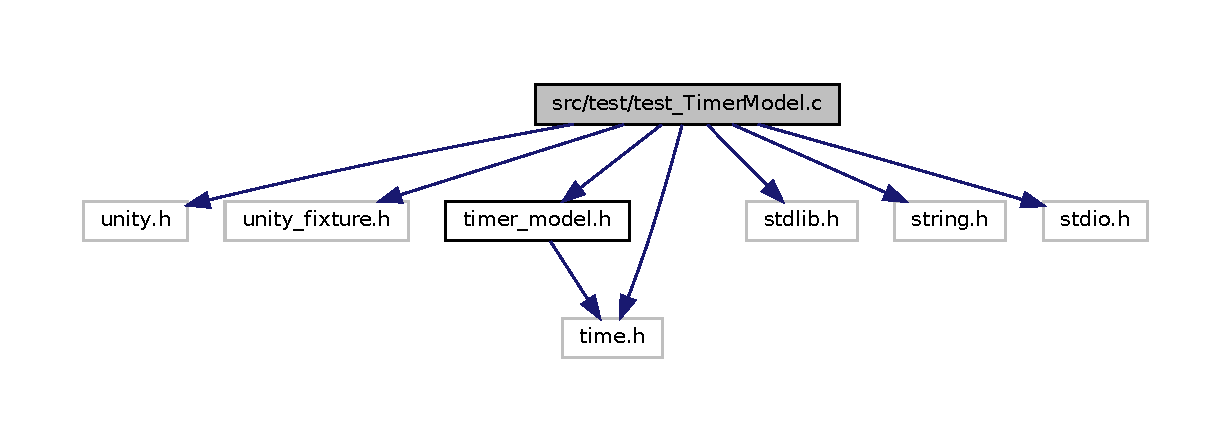
\includegraphics[width=350pt]{test___timer_model_8c__incl}
\end{center}
\end{figure}
\subsection*{Функции}
\begin{DoxyCompactItemize}
\item 
\hyperlink{test___timer_model_8c_a126b01855adcee8a844ee11fcaf4dcb6}{T\+E\+S\+T\+\_\+\+G\+R\+O\+UP} (Test\+Timer\+Model)
\item 
\hyperlink{test___timer_model_8c_a9982d79a153fbc924b2029a1ff98793a}{T\+E\+S\+T\+\_\+\+G\+R\+O\+U\+P\+\_\+\+R\+U\+N\+N\+ER} (Test\+Timer\+Model)
\item 
\hyperlink{test___timer_model_8c_a2d1870b45ddd742650dc88602ffebf21}{T\+E\+S\+T\+\_\+\+S\+E\+T\+UP} (Test\+Timer\+Model)
\item 
\hyperlink{test___timer_model_8c_a0832b54a28c88cf857e2545c5ecbc0e8}{T\+E\+S\+T\+\_\+\+T\+E\+A\+R\+\_\+\+D\+O\+WN} (Test\+Timer\+Model)
\item 
\hyperlink{test___timer_model_8c_a5581ee8b95b7fd50a75e9f24d9aa6128}{T\+E\+ST} (Test\+Timer\+Model, Function\+Create)
\item 
\hyperlink{test___timer_model_8c_a739da8b33240b2e88eea93934fa7e97f}{T\+E\+ST} (Test\+Timer\+Model, Function\+Destroy)
\item 
\hyperlink{test___timer_model_8c_aac89e7cf6d36068a231813ac438c6917}{T\+E\+ST} (Test\+Timer\+Model, Function\+Is\+Start)
\item 
\hyperlink{test___timer_model_8c_a2e8ae6a5bc73e1084329140614facdc4}{T\+E\+ST} (Test\+Timer\+Model, Function\+Save\+Result)
\item 
\hyperlink{test___timer_model_8c_a5b826321b9241a69175c5e368b7993e8}{T\+E\+ST} (Test\+Timer\+Model, Function\+Start)
\item 
\hyperlink{test___timer_model_8c_a0264e684f265cd2ccaa066b2941bf33a}{T\+E\+ST} (Test\+Timer\+Model, Function\+Update)
\end{DoxyCompactItemize}


\subsection{Подробное описание}
Файл тестирующий модель таймеров. 



\subsection{Функции}
\mbox{\Hypertarget{test___timer_model_8c_a5581ee8b95b7fd50a75e9f24d9aa6128}\label{test___timer_model_8c_a5581ee8b95b7fd50a75e9f24d9aa6128}} 
\index{test\+\_\+\+Timer\+Model.\+c@{test\+\_\+\+Timer\+Model.\+c}!T\+E\+ST@{T\+E\+ST}}
\index{T\+E\+ST@{T\+E\+ST}!test\+\_\+\+Timer\+Model.\+c@{test\+\_\+\+Timer\+Model.\+c}}
\subsubsection{\texorpdfstring{T\+E\+S\+T()}{TEST()}\hspace{0.1cm}{\footnotesize\ttfamily [1/6]}}
{\footnotesize\ttfamily T\+E\+ST (\begin{DoxyParamCaption}\item[{Test\+Timer\+Model}]{,  }\item[{Function\+Create}]{ }\end{DoxyParamCaption})}

Функция, которая тестирует функцию timer\+\_\+model\+\_\+create. \mbox{\Hypertarget{test___timer_model_8c_a739da8b33240b2e88eea93934fa7e97f}\label{test___timer_model_8c_a739da8b33240b2e88eea93934fa7e97f}} 
\index{test\+\_\+\+Timer\+Model.\+c@{test\+\_\+\+Timer\+Model.\+c}!T\+E\+ST@{T\+E\+ST}}
\index{T\+E\+ST@{T\+E\+ST}!test\+\_\+\+Timer\+Model.\+c@{test\+\_\+\+Timer\+Model.\+c}}
\subsubsection{\texorpdfstring{T\+E\+S\+T()}{TEST()}\hspace{0.1cm}{\footnotesize\ttfamily [2/6]}}
{\footnotesize\ttfamily T\+E\+ST (\begin{DoxyParamCaption}\item[{Test\+Timer\+Model}]{,  }\item[{Function\+Destroy}]{ }\end{DoxyParamCaption})}

Функция, которая тестирует функцию timer\+\_\+model\+\_\+create. \mbox{\Hypertarget{test___timer_model_8c_aac89e7cf6d36068a231813ac438c6917}\label{test___timer_model_8c_aac89e7cf6d36068a231813ac438c6917}} 
\index{test\+\_\+\+Timer\+Model.\+c@{test\+\_\+\+Timer\+Model.\+c}!T\+E\+ST@{T\+E\+ST}}
\index{T\+E\+ST@{T\+E\+ST}!test\+\_\+\+Timer\+Model.\+c@{test\+\_\+\+Timer\+Model.\+c}}
\subsubsection{\texorpdfstring{T\+E\+S\+T()}{TEST()}\hspace{0.1cm}{\footnotesize\ttfamily [3/6]}}
{\footnotesize\ttfamily T\+E\+ST (\begin{DoxyParamCaption}\item[{Test\+Timer\+Model}]{,  }\item[{Function\+Is\+Start}]{ }\end{DoxyParamCaption})}

Функция, которая тестирует функцию timer\+\_\+model\+\_\+destroy. \mbox{\Hypertarget{test___timer_model_8c_a2e8ae6a5bc73e1084329140614facdc4}\label{test___timer_model_8c_a2e8ae6a5bc73e1084329140614facdc4}} 
\index{test\+\_\+\+Timer\+Model.\+c@{test\+\_\+\+Timer\+Model.\+c}!T\+E\+ST@{T\+E\+ST}}
\index{T\+E\+ST@{T\+E\+ST}!test\+\_\+\+Timer\+Model.\+c@{test\+\_\+\+Timer\+Model.\+c}}
\subsubsection{\texorpdfstring{T\+E\+S\+T()}{TEST()}\hspace{0.1cm}{\footnotesize\ttfamily [4/6]}}
{\footnotesize\ttfamily T\+E\+ST (\begin{DoxyParamCaption}\item[{Test\+Timer\+Model}]{,  }\item[{Function\+Save\+Result}]{ }\end{DoxyParamCaption})}

Функция, которая тестирует функцию timer\+\_\+model\+\_\+save\+\_\+result. \mbox{\Hypertarget{test___timer_model_8c_a5b826321b9241a69175c5e368b7993e8}\label{test___timer_model_8c_a5b826321b9241a69175c5e368b7993e8}} 
\index{test\+\_\+\+Timer\+Model.\+c@{test\+\_\+\+Timer\+Model.\+c}!T\+E\+ST@{T\+E\+ST}}
\index{T\+E\+ST@{T\+E\+ST}!test\+\_\+\+Timer\+Model.\+c@{test\+\_\+\+Timer\+Model.\+c}}
\subsubsection{\texorpdfstring{T\+E\+S\+T()}{TEST()}\hspace{0.1cm}{\footnotesize\ttfamily [5/6]}}
{\footnotesize\ttfamily T\+E\+ST (\begin{DoxyParamCaption}\item[{Test\+Timer\+Model}]{,  }\item[{Function\+Start}]{ }\end{DoxyParamCaption})}

Функция, которая тестирует функцию timer\+\_\+model\+\_\+start. \mbox{\Hypertarget{test___timer_model_8c_a0264e684f265cd2ccaa066b2941bf33a}\label{test___timer_model_8c_a0264e684f265cd2ccaa066b2941bf33a}} 
\index{test\+\_\+\+Timer\+Model.\+c@{test\+\_\+\+Timer\+Model.\+c}!T\+E\+ST@{T\+E\+ST}}
\index{T\+E\+ST@{T\+E\+ST}!test\+\_\+\+Timer\+Model.\+c@{test\+\_\+\+Timer\+Model.\+c}}
\subsubsection{\texorpdfstring{T\+E\+S\+T()}{TEST()}\hspace{0.1cm}{\footnotesize\ttfamily [6/6]}}
{\footnotesize\ttfamily T\+E\+ST (\begin{DoxyParamCaption}\item[{Test\+Timer\+Model}]{,  }\item[{Function\+Update}]{ }\end{DoxyParamCaption})}

Функция, которая тестирует функцию timer\+\_\+model\+\_\+update. \mbox{\Hypertarget{test___timer_model_8c_a126b01855adcee8a844ee11fcaf4dcb6}\label{test___timer_model_8c_a126b01855adcee8a844ee11fcaf4dcb6}} 
\index{test\+\_\+\+Timer\+Model.\+c@{test\+\_\+\+Timer\+Model.\+c}!T\+E\+S\+T\+\_\+\+G\+R\+O\+UP@{T\+E\+S\+T\+\_\+\+G\+R\+O\+UP}}
\index{T\+E\+S\+T\+\_\+\+G\+R\+O\+UP@{T\+E\+S\+T\+\_\+\+G\+R\+O\+UP}!test\+\_\+\+Timer\+Model.\+c@{test\+\_\+\+Timer\+Model.\+c}}
\subsubsection{\texorpdfstring{T\+E\+S\+T\+\_\+\+G\+R\+O\+U\+P()}{TEST\_GROUP()}}
{\footnotesize\ttfamily T\+E\+S\+T\+\_\+\+G\+R\+O\+UP (\begin{DoxyParamCaption}\item[{Test\+Timer\+Model}]{ }\end{DoxyParamCaption})}

\mbox{\Hypertarget{test___timer_model_8c_a9982d79a153fbc924b2029a1ff98793a}\label{test___timer_model_8c_a9982d79a153fbc924b2029a1ff98793a}} 
\index{test\+\_\+\+Timer\+Model.\+c@{test\+\_\+\+Timer\+Model.\+c}!T\+E\+S\+T\+\_\+\+G\+R\+O\+U\+P\+\_\+\+R\+U\+N\+N\+ER@{T\+E\+S\+T\+\_\+\+G\+R\+O\+U\+P\+\_\+\+R\+U\+N\+N\+ER}}
\index{T\+E\+S\+T\+\_\+\+G\+R\+O\+U\+P\+\_\+\+R\+U\+N\+N\+ER@{T\+E\+S\+T\+\_\+\+G\+R\+O\+U\+P\+\_\+\+R\+U\+N\+N\+ER}!test\+\_\+\+Timer\+Model.\+c@{test\+\_\+\+Timer\+Model.\+c}}
\subsubsection{\texorpdfstring{T\+E\+S\+T\+\_\+\+G\+R\+O\+U\+P\+\_\+\+R\+U\+N\+N\+E\+R()}{TEST\_GROUP\_RUNNER()}}
{\footnotesize\ttfamily T\+E\+S\+T\+\_\+\+G\+R\+O\+U\+P\+\_\+\+R\+U\+N\+N\+ER (\begin{DoxyParamCaption}\item[{Test\+Timer\+Model}]{ }\end{DoxyParamCaption})}

\mbox{\Hypertarget{test___timer_model_8c_a2d1870b45ddd742650dc88602ffebf21}\label{test___timer_model_8c_a2d1870b45ddd742650dc88602ffebf21}} 
\index{test\+\_\+\+Timer\+Model.\+c@{test\+\_\+\+Timer\+Model.\+c}!T\+E\+S\+T\+\_\+\+S\+E\+T\+UP@{T\+E\+S\+T\+\_\+\+S\+E\+T\+UP}}
\index{T\+E\+S\+T\+\_\+\+S\+E\+T\+UP@{T\+E\+S\+T\+\_\+\+S\+E\+T\+UP}!test\+\_\+\+Timer\+Model.\+c@{test\+\_\+\+Timer\+Model.\+c}}
\subsubsection{\texorpdfstring{T\+E\+S\+T\+\_\+\+S\+E\+T\+U\+P()}{TEST\_SETUP()}}
{\footnotesize\ttfamily T\+E\+S\+T\+\_\+\+S\+E\+T\+UP (\begin{DoxyParamCaption}\item[{Test\+Timer\+Model}]{ }\end{DoxyParamCaption})}

\mbox{\Hypertarget{test___timer_model_8c_a0832b54a28c88cf857e2545c5ecbc0e8}\label{test___timer_model_8c_a0832b54a28c88cf857e2545c5ecbc0e8}} 
\index{test\+\_\+\+Timer\+Model.\+c@{test\+\_\+\+Timer\+Model.\+c}!T\+E\+S\+T\+\_\+\+T\+E\+A\+R\+\_\+\+D\+O\+WN@{T\+E\+S\+T\+\_\+\+T\+E\+A\+R\+\_\+\+D\+O\+WN}}
\index{T\+E\+S\+T\+\_\+\+T\+E\+A\+R\+\_\+\+D\+O\+WN@{T\+E\+S\+T\+\_\+\+T\+E\+A\+R\+\_\+\+D\+O\+WN}!test\+\_\+\+Timer\+Model.\+c@{test\+\_\+\+Timer\+Model.\+c}}
\subsubsection{\texorpdfstring{T\+E\+S\+T\+\_\+\+T\+E\+A\+R\+\_\+\+D\+O\+W\+N()}{TEST\_TEAR\_DOWN()}}
{\footnotesize\ttfamily T\+E\+S\+T\+\_\+\+T\+E\+A\+R\+\_\+\+D\+O\+WN (\begin{DoxyParamCaption}\item[{Test\+Timer\+Model}]{ }\end{DoxyParamCaption})}


\hypertarget{timer__model_8c}{}\section{Файл src/timer\+\_\+model.c}
\label{timer__model_8c}\index{src/timer\+\_\+model.\+c@{src/timer\+\_\+model.\+c}}
{\ttfamily \#include \char`\"{}timer\+\_\+model.\+h\char`\"{}}\newline
{\ttfamily \#include \char`\"{}error\+\_\+report.\+h\char`\"{}}\newline
{\ttfamily \#include $<$stdio.\+h$>$}\newline
{\ttfamily \#include $<$stdlib.\+h$>$}\newline
{\ttfamily \#include $<$string.\+h$>$}\newline
Граф включаемых заголовочных файлов для timer\+\_\+model.\+c\+:\nopagebreak
\begin{figure}[H]
\begin{center}
\leavevmode
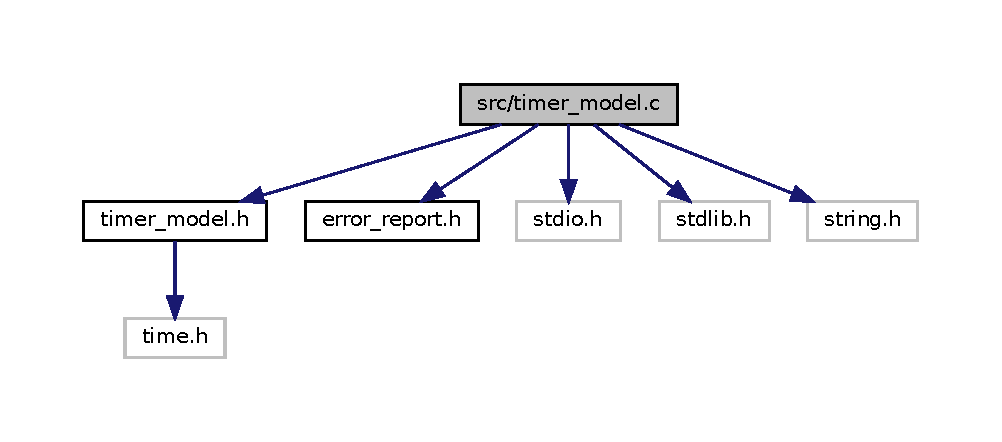
\includegraphics[width=350pt]{timer__model_8c__incl}
\end{center}
\end{figure}
\subsection*{Макросы}
\begin{DoxyCompactItemize}
\item 
\#define \hyperlink{timer__model_8c_ab117546549783a058d0321a287699579}{F\+I\+L\+E\+\_\+\+N\+A\+ME}~\char`\"{}timer\+\_\+model.\+c\char`\"{}
\begin{DoxyCompactList}\small\item\em Имя текущего файла. \end{DoxyCompactList}\item 
\#define \hyperlink{timer__model_8c_a8231167941273d13f41c18f93e945669}{D\+E\+F\+A\+U\+L\+T\+\_\+\+T\+O\+P\+\_\+\+R\+E\+S\+U\+LT}~\char`\"{}Record\+: ??\+:??\char`\"{}
\begin{DoxyCompactList}\small\item\em Строка по умолчанию для рекордного таймера. \end{DoxyCompactList}\item 
\#define \hyperlink{timer__model_8c_a2bbbb638e384ee3b15e3403852d9a220}{S\+E\+C\+\_\+\+I\+N\+\_\+\+MN}~60
\begin{DoxyCompactList}\small\item\em Количество секунд в минуте. \end{DoxyCompactList}\item 
\#define \hyperlink{timer__model_8c_aba64ab31ac50908f7aa4125955fcf2ed}{F\+U\+N\+\_\+\+N\+A\+ME}~\char`\"{}timer\+\_\+model\+\_\+create\char`\"{}
\begin{DoxyCompactList}\small\item\em Имя текущей функции. \end{DoxyCompactList}\item 
\#define \hyperlink{timer__model_8c_aba64ab31ac50908f7aa4125955fcf2ed}{F\+U\+N\+\_\+\+N\+A\+ME}~\char`\"{}timer\+\_\+model\+\_\+start\char`\"{}
\begin{DoxyCompactList}\small\item\em Имя текущей функции. \end{DoxyCompactList}\item 
\#define \hyperlink{timer__model_8c_aba64ab31ac50908f7aa4125955fcf2ed}{F\+U\+N\+\_\+\+N\+A\+ME}~\char`\"{}timer\+\_\+model\+\_\+update\char`\"{}
\begin{DoxyCompactList}\small\item\em Имя текущей функции. \end{DoxyCompactList}\item 
\#define \hyperlink{timer__model_8c_aba64ab31ac50908f7aa4125955fcf2ed}{F\+U\+N\+\_\+\+N\+A\+ME}~\char`\"{}timer\+\_\+model\+\_\+save\+\_\+result\char`\"{}
\begin{DoxyCompactList}\small\item\em Имя текущей функции. \end{DoxyCompactList}\item 
\#define \hyperlink{timer__model_8c_aba64ab31ac50908f7aa4125955fcf2ed}{F\+U\+N\+\_\+\+N\+A\+ME}~\char`\"{}timer\+\_\+model\+\_\+destroy\char`\"{}
\begin{DoxyCompactList}\small\item\em Имя текущей функции. \end{DoxyCompactList}\item 
\#define \hyperlink{timer__model_8c_aba64ab31ac50908f7aa4125955fcf2ed}{F\+U\+N\+\_\+\+N\+A\+ME}~\char`\"{}timer\+\_\+model\+\_\+is\+\_\+start\char`\"{}
\begin{DoxyCompactList}\small\item\em Имя текущей функции. \end{DoxyCompactList}\end{DoxyCompactItemize}
\subsection*{Функции}
\begin{DoxyCompactItemize}
\item 
\hyperlink{structtimer__model}{timer\+\_\+model} $\ast$ \hyperlink{timer__model_8c_a3d025ec0b9a6057b56f8af4f37380bf2}{timer\+\_\+model\+\_\+create} ()
\item 
int \hyperlink{timer__model_8c_a11e6e8d7423a7bb69e61624ec9da4644}{timer\+\_\+model\+\_\+start} (\hyperlink{structtimer__model}{timer\+\_\+model} $\ast$t\+\_\+model)
\item 
int \hyperlink{timer__model_8c_a4e215e6292339c97f3cbfe56a2f1c966}{timer\+\_\+model\+\_\+update} (\hyperlink{structtimer__model}{timer\+\_\+model} $\ast$t\+\_\+model, time\+\_\+t update\+\_\+time)
\item 
int \hyperlink{timer__model_8c_a7c58a0b1d8326901d6cc4e6757bb3639}{timer\+\_\+model\+\_\+save\+\_\+result} (\hyperlink{structtimer__model}{timer\+\_\+model} $\ast$t\+\_\+model)
\item 
int \hyperlink{timer__model_8c_acb3edeec6620f2ed7904d2f8f85d2df8}{timer\+\_\+model\+\_\+destroy} (\hyperlink{structtimer__model}{timer\+\_\+model} $\ast$t\+\_\+model)
\item 
int \hyperlink{timer__model_8c_ad8426e424509fc31990ab0b56202bc2c}{timer\+\_\+model\+\_\+is\+\_\+start} (\hyperlink{structtimer__model}{timer\+\_\+model} $\ast$t\+\_\+model)
\end{DoxyCompactItemize}


\subsection{Макросы}
\mbox{\Hypertarget{timer__model_8c_a8231167941273d13f41c18f93e945669}\label{timer__model_8c_a8231167941273d13f41c18f93e945669}} 
\index{timer\+\_\+model.\+c@{timer\+\_\+model.\+c}!D\+E\+F\+A\+U\+L\+T\+\_\+\+T\+O\+P\+\_\+\+R\+E\+S\+U\+LT@{D\+E\+F\+A\+U\+L\+T\+\_\+\+T\+O\+P\+\_\+\+R\+E\+S\+U\+LT}}
\index{D\+E\+F\+A\+U\+L\+T\+\_\+\+T\+O\+P\+\_\+\+R\+E\+S\+U\+LT@{D\+E\+F\+A\+U\+L\+T\+\_\+\+T\+O\+P\+\_\+\+R\+E\+S\+U\+LT}!timer\+\_\+model.\+c@{timer\+\_\+model.\+c}}
\subsubsection{\texorpdfstring{D\+E\+F\+A\+U\+L\+T\+\_\+\+T\+O\+P\+\_\+\+R\+E\+S\+U\+LT}{DEFAULT\_TOP\_RESULT}}
{\footnotesize\ttfamily \#define D\+E\+F\+A\+U\+L\+T\+\_\+\+T\+O\+P\+\_\+\+R\+E\+S\+U\+LT~\char`\"{}Record\+: ??\+:??\char`\"{}}



Строка по умолчанию для рекордного таймера. 

\mbox{\Hypertarget{timer__model_8c_ab117546549783a058d0321a287699579}\label{timer__model_8c_ab117546549783a058d0321a287699579}} 
\index{timer\+\_\+model.\+c@{timer\+\_\+model.\+c}!F\+I\+L\+E\+\_\+\+N\+A\+ME@{F\+I\+L\+E\+\_\+\+N\+A\+ME}}
\index{F\+I\+L\+E\+\_\+\+N\+A\+ME@{F\+I\+L\+E\+\_\+\+N\+A\+ME}!timer\+\_\+model.\+c@{timer\+\_\+model.\+c}}
\subsubsection{\texorpdfstring{F\+I\+L\+E\+\_\+\+N\+A\+ME}{FILE\_NAME}}
{\footnotesize\ttfamily \#define F\+I\+L\+E\+\_\+\+N\+A\+ME~\char`\"{}timer\+\_\+model.\+c\char`\"{}}



Имя текущего файла. 

\mbox{\Hypertarget{timer__model_8c_aba64ab31ac50908f7aa4125955fcf2ed}\label{timer__model_8c_aba64ab31ac50908f7aa4125955fcf2ed}} 
\index{timer\+\_\+model.\+c@{timer\+\_\+model.\+c}!F\+U\+N\+\_\+\+N\+A\+ME@{F\+U\+N\+\_\+\+N\+A\+ME}}
\index{F\+U\+N\+\_\+\+N\+A\+ME@{F\+U\+N\+\_\+\+N\+A\+ME}!timer\+\_\+model.\+c@{timer\+\_\+model.\+c}}
\subsubsection{\texorpdfstring{F\+U\+N\+\_\+\+N\+A\+ME}{FUN\_NAME}\hspace{0.1cm}{\footnotesize\ttfamily [1/6]}}
{\footnotesize\ttfamily \#define F\+U\+N\+\_\+\+N\+A\+ME~\char`\"{}timer\+\_\+model\+\_\+create\char`\"{}}



Имя текущей функции. 

\mbox{\Hypertarget{timer__model_8c_aba64ab31ac50908f7aa4125955fcf2ed}\label{timer__model_8c_aba64ab31ac50908f7aa4125955fcf2ed}} 
\index{timer\+\_\+model.\+c@{timer\+\_\+model.\+c}!F\+U\+N\+\_\+\+N\+A\+ME@{F\+U\+N\+\_\+\+N\+A\+ME}}
\index{F\+U\+N\+\_\+\+N\+A\+ME@{F\+U\+N\+\_\+\+N\+A\+ME}!timer\+\_\+model.\+c@{timer\+\_\+model.\+c}}
\subsubsection{\texorpdfstring{F\+U\+N\+\_\+\+N\+A\+ME}{FUN\_NAME}\hspace{0.1cm}{\footnotesize\ttfamily [2/6]}}
{\footnotesize\ttfamily \#define F\+U\+N\+\_\+\+N\+A\+ME~\char`\"{}timer\+\_\+model\+\_\+start\char`\"{}}



Имя текущей функции. 

\mbox{\Hypertarget{timer__model_8c_aba64ab31ac50908f7aa4125955fcf2ed}\label{timer__model_8c_aba64ab31ac50908f7aa4125955fcf2ed}} 
\index{timer\+\_\+model.\+c@{timer\+\_\+model.\+c}!F\+U\+N\+\_\+\+N\+A\+ME@{F\+U\+N\+\_\+\+N\+A\+ME}}
\index{F\+U\+N\+\_\+\+N\+A\+ME@{F\+U\+N\+\_\+\+N\+A\+ME}!timer\+\_\+model.\+c@{timer\+\_\+model.\+c}}
\subsubsection{\texorpdfstring{F\+U\+N\+\_\+\+N\+A\+ME}{FUN\_NAME}\hspace{0.1cm}{\footnotesize\ttfamily [3/6]}}
{\footnotesize\ttfamily \#define F\+U\+N\+\_\+\+N\+A\+ME~\char`\"{}timer\+\_\+model\+\_\+update\char`\"{}}



Имя текущей функции. 

\mbox{\Hypertarget{timer__model_8c_aba64ab31ac50908f7aa4125955fcf2ed}\label{timer__model_8c_aba64ab31ac50908f7aa4125955fcf2ed}} 
\index{timer\+\_\+model.\+c@{timer\+\_\+model.\+c}!F\+U\+N\+\_\+\+N\+A\+ME@{F\+U\+N\+\_\+\+N\+A\+ME}}
\index{F\+U\+N\+\_\+\+N\+A\+ME@{F\+U\+N\+\_\+\+N\+A\+ME}!timer\+\_\+model.\+c@{timer\+\_\+model.\+c}}
\subsubsection{\texorpdfstring{F\+U\+N\+\_\+\+N\+A\+ME}{FUN\_NAME}\hspace{0.1cm}{\footnotesize\ttfamily [4/6]}}
{\footnotesize\ttfamily \#define F\+U\+N\+\_\+\+N\+A\+ME~\char`\"{}timer\+\_\+model\+\_\+save\+\_\+result\char`\"{}}



Имя текущей функции. 

\mbox{\Hypertarget{timer__model_8c_aba64ab31ac50908f7aa4125955fcf2ed}\label{timer__model_8c_aba64ab31ac50908f7aa4125955fcf2ed}} 
\index{timer\+\_\+model.\+c@{timer\+\_\+model.\+c}!F\+U\+N\+\_\+\+N\+A\+ME@{F\+U\+N\+\_\+\+N\+A\+ME}}
\index{F\+U\+N\+\_\+\+N\+A\+ME@{F\+U\+N\+\_\+\+N\+A\+ME}!timer\+\_\+model.\+c@{timer\+\_\+model.\+c}}
\subsubsection{\texorpdfstring{F\+U\+N\+\_\+\+N\+A\+ME}{FUN\_NAME}\hspace{0.1cm}{\footnotesize\ttfamily [5/6]}}
{\footnotesize\ttfamily \#define F\+U\+N\+\_\+\+N\+A\+ME~\char`\"{}timer\+\_\+model\+\_\+destroy\char`\"{}}



Имя текущей функции. 

\mbox{\Hypertarget{timer__model_8c_aba64ab31ac50908f7aa4125955fcf2ed}\label{timer__model_8c_aba64ab31ac50908f7aa4125955fcf2ed}} 
\index{timer\+\_\+model.\+c@{timer\+\_\+model.\+c}!F\+U\+N\+\_\+\+N\+A\+ME@{F\+U\+N\+\_\+\+N\+A\+ME}}
\index{F\+U\+N\+\_\+\+N\+A\+ME@{F\+U\+N\+\_\+\+N\+A\+ME}!timer\+\_\+model.\+c@{timer\+\_\+model.\+c}}
\subsubsection{\texorpdfstring{F\+U\+N\+\_\+\+N\+A\+ME}{FUN\_NAME}\hspace{0.1cm}{\footnotesize\ttfamily [6/6]}}
{\footnotesize\ttfamily \#define F\+U\+N\+\_\+\+N\+A\+ME~\char`\"{}timer\+\_\+model\+\_\+is\+\_\+start\char`\"{}}



Имя текущей функции. 

\mbox{\Hypertarget{timer__model_8c_a2bbbb638e384ee3b15e3403852d9a220}\label{timer__model_8c_a2bbbb638e384ee3b15e3403852d9a220}} 
\index{timer\+\_\+model.\+c@{timer\+\_\+model.\+c}!S\+E\+C\+\_\+\+I\+N\+\_\+\+MN@{S\+E\+C\+\_\+\+I\+N\+\_\+\+MN}}
\index{S\+E\+C\+\_\+\+I\+N\+\_\+\+MN@{S\+E\+C\+\_\+\+I\+N\+\_\+\+MN}!timer\+\_\+model.\+c@{timer\+\_\+model.\+c}}
\subsubsection{\texorpdfstring{S\+E\+C\+\_\+\+I\+N\+\_\+\+MN}{SEC\_IN\_MN}}
{\footnotesize\ttfamily \#define S\+E\+C\+\_\+\+I\+N\+\_\+\+MN~60}



Количество секунд в минуте. 



\subsection{Функции}
\mbox{\Hypertarget{timer__model_8c_a3d025ec0b9a6057b56f8af4f37380bf2}\label{timer__model_8c_a3d025ec0b9a6057b56f8af4f37380bf2}} 
\index{timer\+\_\+model.\+c@{timer\+\_\+model.\+c}!timer\+\_\+model\+\_\+create@{timer\+\_\+model\+\_\+create}}
\index{timer\+\_\+model\+\_\+create@{timer\+\_\+model\+\_\+create}!timer\+\_\+model.\+c@{timer\+\_\+model.\+c}}
\subsubsection{\texorpdfstring{timer\+\_\+model\+\_\+create()}{timer\_model\_create()}}
{\footnotesize\ttfamily \hyperlink{structtimer__model}{timer\+\_\+model}$\ast$ timer\+\_\+model\+\_\+create (\begin{DoxyParamCaption}{ }\end{DoxyParamCaption})}

Создание модели таймера. \begin{DoxyReturn}{Возвращает}
Адрес, созданной модели. ~\newline
 N\+U\+LL, если во время создания модели произошла ошибка. 
\end{DoxyReturn}
\mbox{\Hypertarget{timer__model_8c_acb3edeec6620f2ed7904d2f8f85d2df8}\label{timer__model_8c_acb3edeec6620f2ed7904d2f8f85d2df8}} 
\index{timer\+\_\+model.\+c@{timer\+\_\+model.\+c}!timer\+\_\+model\+\_\+destroy@{timer\+\_\+model\+\_\+destroy}}
\index{timer\+\_\+model\+\_\+destroy@{timer\+\_\+model\+\_\+destroy}!timer\+\_\+model.\+c@{timer\+\_\+model.\+c}}
\subsubsection{\texorpdfstring{timer\+\_\+model\+\_\+destroy()}{timer\_model\_destroy()}}
{\footnotesize\ttfamily int timer\+\_\+model\+\_\+destroy (\begin{DoxyParamCaption}\item[{\hyperlink{structtimer__model}{timer\+\_\+model} $\ast$}]{t\+\_\+model }\end{DoxyParamCaption})}

Удаление модели таймера. 
\begin{DoxyParams}[1]{Аргументы}
\mbox{\tt in}  & {\em t\+\_\+model} & -\/ адрес модели таймера, которую нужно удалить. \\
\hline
\end{DoxyParams}
\begin{DoxyReturn}{Возвращает}
Ноль, если удаление прошло успешно. ~\newline
 Ненулевое число, если во время удаления произошла ошибка. 
\end{DoxyReturn}
\mbox{\Hypertarget{timer__model_8c_ad8426e424509fc31990ab0b56202bc2c}\label{timer__model_8c_ad8426e424509fc31990ab0b56202bc2c}} 
\index{timer\+\_\+model.\+c@{timer\+\_\+model.\+c}!timer\+\_\+model\+\_\+is\+\_\+start@{timer\+\_\+model\+\_\+is\+\_\+start}}
\index{timer\+\_\+model\+\_\+is\+\_\+start@{timer\+\_\+model\+\_\+is\+\_\+start}!timer\+\_\+model.\+c@{timer\+\_\+model.\+c}}
\subsubsection{\texorpdfstring{timer\+\_\+model\+\_\+is\+\_\+start()}{timer\_model\_is\_start()}}
{\footnotesize\ttfamily int timer\+\_\+model\+\_\+is\+\_\+start (\begin{DoxyParamCaption}\item[{\hyperlink{structtimer__model}{timer\+\_\+model} $\ast$}]{t\+\_\+model }\end{DoxyParamCaption})}

Проверка запуска таймера. 
\begin{DoxyParams}[1]{Аргументы}
\mbox{\tt in}  & {\em t\+\_\+model} & -\/ адрес модели таймера, которую нужно проверить. \\
\hline
\end{DoxyParams}
\begin{DoxyReturn}{Возвращает}
Отрицательное число, если во время проверки произошла ошибка. ~\newline
 Ноль, если таймер не запущен. ~\newline
 Положительное число, если таймер запущен. 
\end{DoxyReturn}
\mbox{\Hypertarget{timer__model_8c_a7c58a0b1d8326901d6cc4e6757bb3639}\label{timer__model_8c_a7c58a0b1d8326901d6cc4e6757bb3639}} 
\index{timer\+\_\+model.\+c@{timer\+\_\+model.\+c}!timer\+\_\+model\+\_\+save\+\_\+result@{timer\+\_\+model\+\_\+save\+\_\+result}}
\index{timer\+\_\+model\+\_\+save\+\_\+result@{timer\+\_\+model\+\_\+save\+\_\+result}!timer\+\_\+model.\+c@{timer\+\_\+model.\+c}}
\subsubsection{\texorpdfstring{timer\+\_\+model\+\_\+save\+\_\+result()}{timer\_model\_save\_result()}}
{\footnotesize\ttfamily int timer\+\_\+model\+\_\+save\+\_\+result (\begin{DoxyParamCaption}\item[{\hyperlink{structtimer__model}{timer\+\_\+model} $\ast$}]{t\+\_\+model }\end{DoxyParamCaption})}

Сохранение рекорда. 
\begin{DoxyParams}[1]{Аргументы}
\mbox{\tt in}  & {\em t\+\_\+model} & -\/ адрес модели таймера, рекорд которой нужно сохранить. \\
\hline
\end{DoxyParams}
\begin{DoxyReturn}{Возвращает}
Ноль, если сохранение прошло успешно. ~\newline
 Ненулевое число, если во время сохранения произошла ошибка. 
\end{DoxyReturn}
\mbox{\Hypertarget{timer__model_8c_a11e6e8d7423a7bb69e61624ec9da4644}\label{timer__model_8c_a11e6e8d7423a7bb69e61624ec9da4644}} 
\index{timer\+\_\+model.\+c@{timer\+\_\+model.\+c}!timer\+\_\+model\+\_\+start@{timer\+\_\+model\+\_\+start}}
\index{timer\+\_\+model\+\_\+start@{timer\+\_\+model\+\_\+start}!timer\+\_\+model.\+c@{timer\+\_\+model.\+c}}
\subsubsection{\texorpdfstring{timer\+\_\+model\+\_\+start()}{timer\_model\_start()}}
{\footnotesize\ttfamily int timer\+\_\+model\+\_\+start (\begin{DoxyParamCaption}\item[{\hyperlink{structtimer__model}{timer\+\_\+model} $\ast$}]{t\+\_\+model }\end{DoxyParamCaption})}

Пуск таймера. 
\begin{DoxyParams}[1]{Аргументы}
\mbox{\tt in,out}  & {\em t\+\_\+model} & -\/ адрес модели таймера, который нужно запустить. \\
\hline
\end{DoxyParams}
\begin{DoxyReturn}{Возвращает}
Ноль, если запуск прошёл успешно. ~\newline
 Ненулевое число, если во время запуска произошла ошибка. 
\end{DoxyReturn}
\mbox{\Hypertarget{timer__model_8c_a4e215e6292339c97f3cbfe56a2f1c966}\label{timer__model_8c_a4e215e6292339c97f3cbfe56a2f1c966}} 
\index{timer\+\_\+model.\+c@{timer\+\_\+model.\+c}!timer\+\_\+model\+\_\+update@{timer\+\_\+model\+\_\+update}}
\index{timer\+\_\+model\+\_\+update@{timer\+\_\+model\+\_\+update}!timer\+\_\+model.\+c@{timer\+\_\+model.\+c}}
\subsubsection{\texorpdfstring{timer\+\_\+model\+\_\+update()}{timer\_model\_update()}}
{\footnotesize\ttfamily int timer\+\_\+model\+\_\+update (\begin{DoxyParamCaption}\item[{\hyperlink{structtimer__model}{timer\+\_\+model} $\ast$}]{t\+\_\+model,  }\item[{time\+\_\+t}]{update\+\_\+time }\end{DoxyParamCaption})}

Обновление данных модели таймера. 
\begin{DoxyParams}[1]{Аргументы}
\mbox{\tt in,out}  & {\em t\+\_\+model} & -\/ адрес модели таймера, которую необходимо обновить. \\
\hline
\mbox{\tt in}  & {\em update\+\_\+time} & -\/ время, в которое происходит обновление. \\
\hline
\end{DoxyParams}
\begin{DoxyReturn}{Возвращает}
Ноль, если обновление прошло успешно. ~\newline
 Ненулевое число, если во время обновления произошла ошибка. 
\end{DoxyReturn}

\hypertarget{timer__model_8h}{}\section{Файл src/timer\+\_\+model.h}
\label{timer__model_8h}\index{src/timer\+\_\+model.\+h@{src/timer\+\_\+model.\+h}}


Файл, в котором опеределены функции для работы с моделью таймеров.  


{\ttfamily \#include $<$time.\+h$>$}\newline
Граф включаемых заголовочных файлов для timer\+\_\+model.\+h\+:\nopagebreak
\begin{figure}[H]
\begin{center}
\leavevmode
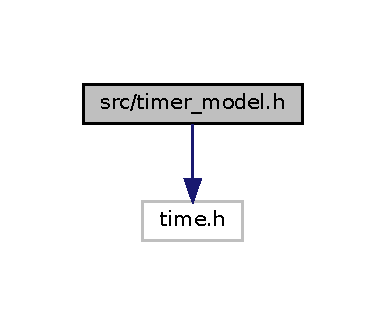
\includegraphics[width=185pt]{timer__model_8h__incl}
\end{center}
\end{figure}
Граф файлов, в которые включается этот файл\+:\nopagebreak
\begin{figure}[H]
\begin{center}
\leavevmode
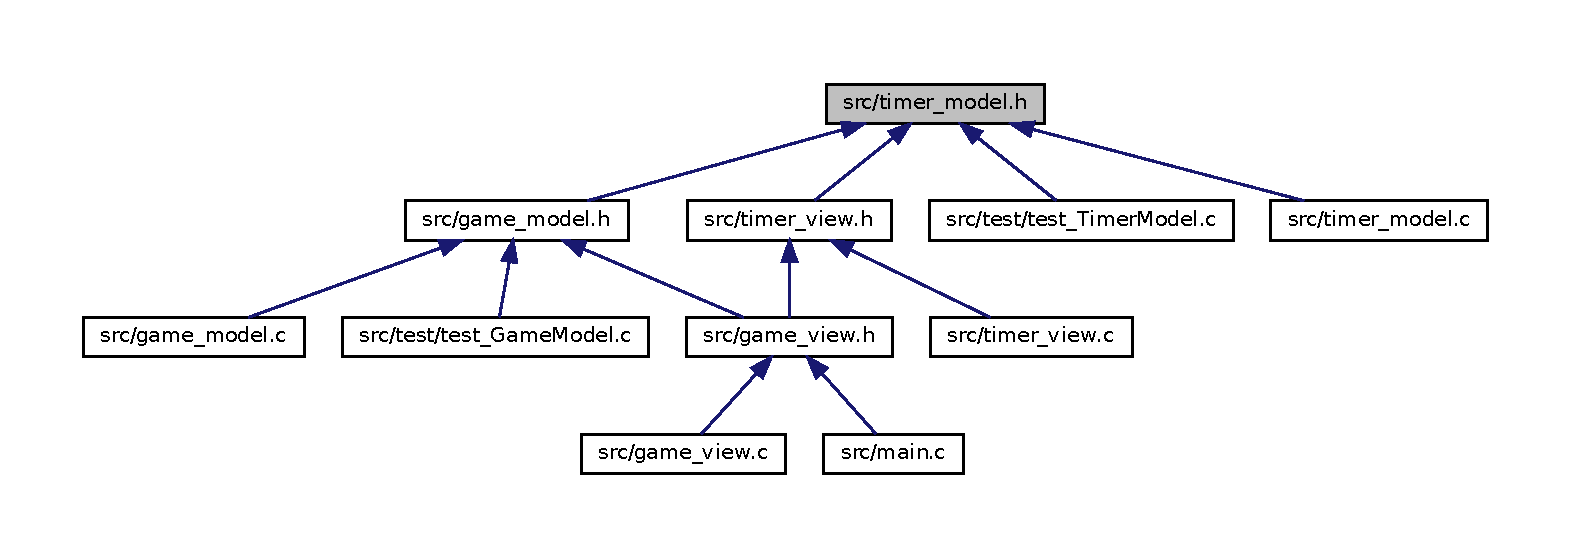
\includegraphics[width=350pt]{timer__model_8h__dep__incl}
\end{center}
\end{figure}
\subsection*{Структуры данных}
\begin{DoxyCompactItemize}
\item 
struct \hyperlink{structtimer__model}{timer\+\_\+model}
\begin{DoxyCompactList}\small\item\em Структура, которая описывает модель таймеров. \end{DoxyCompactList}\end{DoxyCompactItemize}
\subsection*{Макросы}
\begin{DoxyCompactItemize}
\item 
\#define \hyperlink{timer__model_8h_a48a3a050ba862a07c3df89c738dcaa3b}{P\+A\+T\+H\+\_\+\+D\+A\+TA}~\char`\"{}res/record\+\_\+time.\+txt\char`\"{}
\begin{DoxyCompactList}\small\item\em Путь к файлу с лучшим рекордным временем. \end{DoxyCompactList}\item 
\#define \hyperlink{timer__model_8h_afb8e0513b4926ca94b38be5d60aaf125}{S\+I\+Z\+E\+\_\+\+T\+I\+M\+E\+\_\+\+S\+T\+R\+I\+NG}~20
\begin{DoxyCompactList}\small\item\em Максимальный размер строки, в которой хранятся данные таймеров. \end{DoxyCompactList}\item 
\#define \hyperlink{timer__model_8h_a5ff1ef7bd6c1df2a650162766a2ddb76}{M\+A\+X\+\_\+\+MN}~60
\begin{DoxyCompactList}\small\item\em Максимальное количество минут измеряемое таймером. \end{DoxyCompactList}\item 
\#define \hyperlink{timer__model_8h_ab96c94c7d4f72592fb0bd579675c89f2}{M\+A\+X\+\_\+\+S\+EC}~59
\begin{DoxyCompactList}\small\item\em Максимальное количество секунд измеряемое таймером. \end{DoxyCompactList}\end{DoxyCompactItemize}
\subsection*{Определения типов}
\begin{DoxyCompactItemize}
\item 
typedef struct \hyperlink{structtimer__model}{timer\+\_\+model} \hyperlink{timer__model_8h_a3d7afc678136b4c2a7a91c795bec954f}{timer\+\_\+model}
\end{DoxyCompactItemize}
\subsection*{Функции}
\begin{DoxyCompactItemize}
\item 
\hyperlink{structtimer__model}{timer\+\_\+model} $\ast$ \hyperlink{timer__model_8h_a3d025ec0b9a6057b56f8af4f37380bf2}{timer\+\_\+model\+\_\+create} ()
\item 
int \hyperlink{timer__model_8h_a11e6e8d7423a7bb69e61624ec9da4644}{timer\+\_\+model\+\_\+start} (\hyperlink{structtimer__model}{timer\+\_\+model} $\ast$t\+\_\+model)
\item 
int \hyperlink{timer__model_8h_a4e215e6292339c97f3cbfe56a2f1c966}{timer\+\_\+model\+\_\+update} (\hyperlink{structtimer__model}{timer\+\_\+model} $\ast$t\+\_\+model, time\+\_\+t update\+\_\+time)
\item 
int \hyperlink{timer__model_8h_a7c58a0b1d8326901d6cc4e6757bb3639}{timer\+\_\+model\+\_\+save\+\_\+result} (\hyperlink{structtimer__model}{timer\+\_\+model} $\ast$t\+\_\+model)
\item 
int \hyperlink{timer__model_8h_acb3edeec6620f2ed7904d2f8f85d2df8}{timer\+\_\+model\+\_\+destroy} (\hyperlink{structtimer__model}{timer\+\_\+model} $\ast$t\+\_\+model)
\item 
int \hyperlink{timer__model_8h_ad8426e424509fc31990ab0b56202bc2c}{timer\+\_\+model\+\_\+is\+\_\+start} (\hyperlink{structtimer__model}{timer\+\_\+model} $\ast$t\+\_\+model)
\end{DoxyCompactItemize}


\subsection{Подробное описание}
Файл, в котором опеределены функции для работы с моделью таймеров. 



\subsection{Макросы}
\mbox{\Hypertarget{timer__model_8h_a5ff1ef7bd6c1df2a650162766a2ddb76}\label{timer__model_8h_a5ff1ef7bd6c1df2a650162766a2ddb76}} 
\index{timer\+\_\+model.\+h@{timer\+\_\+model.\+h}!M\+A\+X\+\_\+\+MN@{M\+A\+X\+\_\+\+MN}}
\index{M\+A\+X\+\_\+\+MN@{M\+A\+X\+\_\+\+MN}!timer\+\_\+model.\+h@{timer\+\_\+model.\+h}}
\subsubsection{\texorpdfstring{M\+A\+X\+\_\+\+MN}{MAX\_MN}}
{\footnotesize\ttfamily \#define M\+A\+X\+\_\+\+MN~60}



Максимальное количество минут измеряемое таймером. 

\mbox{\Hypertarget{timer__model_8h_ab96c94c7d4f72592fb0bd579675c89f2}\label{timer__model_8h_ab96c94c7d4f72592fb0bd579675c89f2}} 
\index{timer\+\_\+model.\+h@{timer\+\_\+model.\+h}!M\+A\+X\+\_\+\+S\+EC@{M\+A\+X\+\_\+\+S\+EC}}
\index{M\+A\+X\+\_\+\+S\+EC@{M\+A\+X\+\_\+\+S\+EC}!timer\+\_\+model.\+h@{timer\+\_\+model.\+h}}
\subsubsection{\texorpdfstring{M\+A\+X\+\_\+\+S\+EC}{MAX\_SEC}}
{\footnotesize\ttfamily \#define M\+A\+X\+\_\+\+S\+EC~59}



Максимальное количество секунд измеряемое таймером. 

\mbox{\Hypertarget{timer__model_8h_a48a3a050ba862a07c3df89c738dcaa3b}\label{timer__model_8h_a48a3a050ba862a07c3df89c738dcaa3b}} 
\index{timer\+\_\+model.\+h@{timer\+\_\+model.\+h}!P\+A\+T\+H\+\_\+\+D\+A\+TA@{P\+A\+T\+H\+\_\+\+D\+A\+TA}}
\index{P\+A\+T\+H\+\_\+\+D\+A\+TA@{P\+A\+T\+H\+\_\+\+D\+A\+TA}!timer\+\_\+model.\+h@{timer\+\_\+model.\+h}}
\subsubsection{\texorpdfstring{P\+A\+T\+H\+\_\+\+D\+A\+TA}{PATH\_DATA}}
{\footnotesize\ttfamily \#define P\+A\+T\+H\+\_\+\+D\+A\+TA~\char`\"{}res/record\+\_\+time.\+txt\char`\"{}}



Путь к файлу с лучшим рекордным временем. 

\mbox{\Hypertarget{timer__model_8h_afb8e0513b4926ca94b38be5d60aaf125}\label{timer__model_8h_afb8e0513b4926ca94b38be5d60aaf125}} 
\index{timer\+\_\+model.\+h@{timer\+\_\+model.\+h}!S\+I\+Z\+E\+\_\+\+T\+I\+M\+E\+\_\+\+S\+T\+R\+I\+NG@{S\+I\+Z\+E\+\_\+\+T\+I\+M\+E\+\_\+\+S\+T\+R\+I\+NG}}
\index{S\+I\+Z\+E\+\_\+\+T\+I\+M\+E\+\_\+\+S\+T\+R\+I\+NG@{S\+I\+Z\+E\+\_\+\+T\+I\+M\+E\+\_\+\+S\+T\+R\+I\+NG}!timer\+\_\+model.\+h@{timer\+\_\+model.\+h}}
\subsubsection{\texorpdfstring{S\+I\+Z\+E\+\_\+\+T\+I\+M\+E\+\_\+\+S\+T\+R\+I\+NG}{SIZE\_TIME\_STRING}}
{\footnotesize\ttfamily \#define S\+I\+Z\+E\+\_\+\+T\+I\+M\+E\+\_\+\+S\+T\+R\+I\+NG~20}



Максимальный размер строки, в которой хранятся данные таймеров. 



\subsection{Типы}
\mbox{\Hypertarget{timer__model_8h_a3d7afc678136b4c2a7a91c795bec954f}\label{timer__model_8h_a3d7afc678136b4c2a7a91c795bec954f}} 
\index{timer\+\_\+model.\+h@{timer\+\_\+model.\+h}!timer\+\_\+model@{timer\+\_\+model}}
\index{timer\+\_\+model@{timer\+\_\+model}!timer\+\_\+model.\+h@{timer\+\_\+model.\+h}}
\subsubsection{\texorpdfstring{timer\+\_\+model}{timer\_model}}
{\footnotesize\ttfamily typedef struct \hyperlink{structtimer__model}{timer\+\_\+model} \hyperlink{structtimer__model}{timer\+\_\+model}}



\subsection{Функции}
\mbox{\Hypertarget{timer__model_8h_a3d025ec0b9a6057b56f8af4f37380bf2}\label{timer__model_8h_a3d025ec0b9a6057b56f8af4f37380bf2}} 
\index{timer\+\_\+model.\+h@{timer\+\_\+model.\+h}!timer\+\_\+model\+\_\+create@{timer\+\_\+model\+\_\+create}}
\index{timer\+\_\+model\+\_\+create@{timer\+\_\+model\+\_\+create}!timer\+\_\+model.\+h@{timer\+\_\+model.\+h}}
\subsubsection{\texorpdfstring{timer\+\_\+model\+\_\+create()}{timer\_model\_create()}}
{\footnotesize\ttfamily \hyperlink{structtimer__model}{timer\+\_\+model}$\ast$ timer\+\_\+model\+\_\+create (\begin{DoxyParamCaption}{ }\end{DoxyParamCaption})}

Создание модели таймера. \begin{DoxyReturn}{Возвращает}
Адрес, созданной модели. ~\newline
 N\+U\+LL, если во время создания модели произошла ошибка. 
\end{DoxyReturn}
\mbox{\Hypertarget{timer__model_8h_acb3edeec6620f2ed7904d2f8f85d2df8}\label{timer__model_8h_acb3edeec6620f2ed7904d2f8f85d2df8}} 
\index{timer\+\_\+model.\+h@{timer\+\_\+model.\+h}!timer\+\_\+model\+\_\+destroy@{timer\+\_\+model\+\_\+destroy}}
\index{timer\+\_\+model\+\_\+destroy@{timer\+\_\+model\+\_\+destroy}!timer\+\_\+model.\+h@{timer\+\_\+model.\+h}}
\subsubsection{\texorpdfstring{timer\+\_\+model\+\_\+destroy()}{timer\_model\_destroy()}}
{\footnotesize\ttfamily int timer\+\_\+model\+\_\+destroy (\begin{DoxyParamCaption}\item[{\hyperlink{structtimer__model}{timer\+\_\+model} $\ast$}]{t\+\_\+model }\end{DoxyParamCaption})}

Удаление модели таймера. 
\begin{DoxyParams}[1]{Аргументы}
\mbox{\tt in}  & {\em t\+\_\+model} & -\/ адрес модели таймера, которую нужно удалить. \\
\hline
\end{DoxyParams}
\begin{DoxyReturn}{Возвращает}
Ноль, если удаление прошло успешно. ~\newline
 Ненулевое число, если во время удаления произошла ошибка. 
\end{DoxyReturn}
\mbox{\Hypertarget{timer__model_8h_ad8426e424509fc31990ab0b56202bc2c}\label{timer__model_8h_ad8426e424509fc31990ab0b56202bc2c}} 
\index{timer\+\_\+model.\+h@{timer\+\_\+model.\+h}!timer\+\_\+model\+\_\+is\+\_\+start@{timer\+\_\+model\+\_\+is\+\_\+start}}
\index{timer\+\_\+model\+\_\+is\+\_\+start@{timer\+\_\+model\+\_\+is\+\_\+start}!timer\+\_\+model.\+h@{timer\+\_\+model.\+h}}
\subsubsection{\texorpdfstring{timer\+\_\+model\+\_\+is\+\_\+start()}{timer\_model\_is\_start()}}
{\footnotesize\ttfamily int timer\+\_\+model\+\_\+is\+\_\+start (\begin{DoxyParamCaption}\item[{\hyperlink{structtimer__model}{timer\+\_\+model} $\ast$}]{t\+\_\+model }\end{DoxyParamCaption})}

Проверка запуска таймера. 
\begin{DoxyParams}[1]{Аргументы}
\mbox{\tt in}  & {\em t\+\_\+model} & -\/ адрес модели таймера, которую нужно проверить. \\
\hline
\end{DoxyParams}
\begin{DoxyReturn}{Возвращает}
Отрицательное число, если во время проверки произошла ошибка. ~\newline
 Ноль, если таймер не запущен. ~\newline
 Положительное число, если таймер запущен. 
\end{DoxyReturn}
\mbox{\Hypertarget{timer__model_8h_a7c58a0b1d8326901d6cc4e6757bb3639}\label{timer__model_8h_a7c58a0b1d8326901d6cc4e6757bb3639}} 
\index{timer\+\_\+model.\+h@{timer\+\_\+model.\+h}!timer\+\_\+model\+\_\+save\+\_\+result@{timer\+\_\+model\+\_\+save\+\_\+result}}
\index{timer\+\_\+model\+\_\+save\+\_\+result@{timer\+\_\+model\+\_\+save\+\_\+result}!timer\+\_\+model.\+h@{timer\+\_\+model.\+h}}
\subsubsection{\texorpdfstring{timer\+\_\+model\+\_\+save\+\_\+result()}{timer\_model\_save\_result()}}
{\footnotesize\ttfamily int timer\+\_\+model\+\_\+save\+\_\+result (\begin{DoxyParamCaption}\item[{\hyperlink{structtimer__model}{timer\+\_\+model} $\ast$}]{t\+\_\+model }\end{DoxyParamCaption})}

Сохранение рекорда. 
\begin{DoxyParams}[1]{Аргументы}
\mbox{\tt in}  & {\em t\+\_\+model} & -\/ адрес модели таймера, рекорд которой нужно сохранить. \\
\hline
\end{DoxyParams}
\begin{DoxyReturn}{Возвращает}
Ноль, если сохранение прошло успешно. ~\newline
 Ненулевое число, если во время сохранения произошла ошибка. 
\end{DoxyReturn}
\mbox{\Hypertarget{timer__model_8h_a11e6e8d7423a7bb69e61624ec9da4644}\label{timer__model_8h_a11e6e8d7423a7bb69e61624ec9da4644}} 
\index{timer\+\_\+model.\+h@{timer\+\_\+model.\+h}!timer\+\_\+model\+\_\+start@{timer\+\_\+model\+\_\+start}}
\index{timer\+\_\+model\+\_\+start@{timer\+\_\+model\+\_\+start}!timer\+\_\+model.\+h@{timer\+\_\+model.\+h}}
\subsubsection{\texorpdfstring{timer\+\_\+model\+\_\+start()}{timer\_model\_start()}}
{\footnotesize\ttfamily int timer\+\_\+model\+\_\+start (\begin{DoxyParamCaption}\item[{\hyperlink{structtimer__model}{timer\+\_\+model} $\ast$}]{t\+\_\+model }\end{DoxyParamCaption})}

Пуск таймера. 
\begin{DoxyParams}[1]{Аргументы}
\mbox{\tt in,out}  & {\em t\+\_\+model} & -\/ адрес модели таймера, который нужно запустить. \\
\hline
\end{DoxyParams}
\begin{DoxyReturn}{Возвращает}
Ноль, если запуск прошёл успешно. ~\newline
 Ненулевое число, если во время запуска произошла ошибка. 
\end{DoxyReturn}
\mbox{\Hypertarget{timer__model_8h_a4e215e6292339c97f3cbfe56a2f1c966}\label{timer__model_8h_a4e215e6292339c97f3cbfe56a2f1c966}} 
\index{timer\+\_\+model.\+h@{timer\+\_\+model.\+h}!timer\+\_\+model\+\_\+update@{timer\+\_\+model\+\_\+update}}
\index{timer\+\_\+model\+\_\+update@{timer\+\_\+model\+\_\+update}!timer\+\_\+model.\+h@{timer\+\_\+model.\+h}}
\subsubsection{\texorpdfstring{timer\+\_\+model\+\_\+update()}{timer\_model\_update()}}
{\footnotesize\ttfamily int timer\+\_\+model\+\_\+update (\begin{DoxyParamCaption}\item[{\hyperlink{structtimer__model}{timer\+\_\+model} $\ast$}]{t\+\_\+model,  }\item[{time\+\_\+t}]{update\+\_\+time }\end{DoxyParamCaption})}

Обновление данных модели таймера. 
\begin{DoxyParams}[1]{Аргументы}
\mbox{\tt in,out}  & {\em t\+\_\+model} & -\/ адрес модели таймера, которую необходимо обновить. \\
\hline
\mbox{\tt in}  & {\em update\+\_\+time} & -\/ время, в которое происходит обновление. \\
\hline
\end{DoxyParams}
\begin{DoxyReturn}{Возвращает}
Ноль, если обновление прошло успешно. ~\newline
 Ненулевое число, если во время обновления произошла ошибка. 
\end{DoxyReturn}

\hypertarget{timer__view_8c}{}\section{Файл src/timer\+\_\+view.c}
\label{timer__view_8c}\index{src/timer\+\_\+view.\+c@{src/timer\+\_\+view.\+c}}


Файл, в котором реализованы функции для работы с отображением таймеров.  


{\ttfamily \#include \char`\"{}timer\+\_\+view.\+h\char`\"{}}\newline
{\ttfamily \#include \char`\"{}error\+\_\+report.\+h\char`\"{}}\newline
{\ttfamily \#include $<$stdlib.\+h$>$}\newline
Граф включаемых заголовочных файлов для timer\+\_\+view.\+c\+:\nopagebreak
\begin{figure}[H]
\begin{center}
\leavevmode
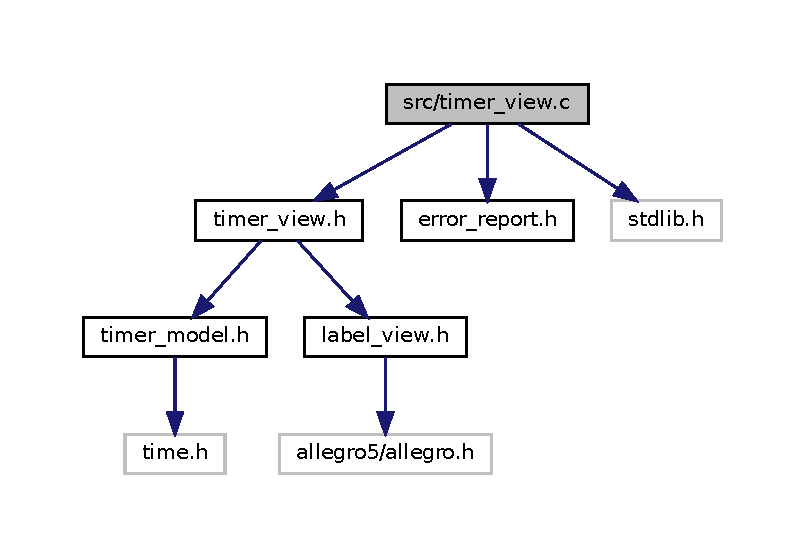
\includegraphics[width=350pt]{timer__view_8c__incl}
\end{center}
\end{figure}
\subsection*{Макросы}
\begin{DoxyCompactItemize}
\item 
\#define \hyperlink{timer__view_8c_ab117546549783a058d0321a287699579}{F\+I\+L\+E\+\_\+\+N\+A\+ME}~\char`\"{}timer\+\_\+view.\+c\char`\"{}
\begin{DoxyCompactList}\small\item\em Текущие имя файла. \end{DoxyCompactList}\item 
\#define \hyperlink{timer__view_8c_aba64ab31ac50908f7aa4125955fcf2ed}{F\+U\+N\+\_\+\+N\+A\+ME}~\char`\"{}timer\+\_\+view\+\_\+create\char`\"{}
\begin{DoxyCompactList}\small\item\em Имя текущей функции. \end{DoxyCompactList}\item 
\#define \hyperlink{timer__view_8c_aba64ab31ac50908f7aa4125955fcf2ed}{F\+U\+N\+\_\+\+N\+A\+ME}~\char`\"{}timer\+\_\+view\+\_\+draw\char`\"{}
\begin{DoxyCompactList}\small\item\em Имя текущей функции. \end{DoxyCompactList}\item 
\#define \hyperlink{timer__view_8c_aba64ab31ac50908f7aa4125955fcf2ed}{F\+U\+N\+\_\+\+N\+A\+ME}~\char`\"{}timer\+\_\+view\+\_\+destroy\char`\"{}
\begin{DoxyCompactList}\small\item\em Имя текущей функции. \end{DoxyCompactList}\end{DoxyCompactItemize}
\subsection*{Функции}
\begin{DoxyCompactItemize}
\item 
\hyperlink{structtimer__view}{timer\+\_\+view} $\ast$ \hyperlink{timer__view_8c_ab60c31593d649a049480639234e40c3b}{timer\+\_\+view\+\_\+create} (\hyperlink{structtimer__model}{timer\+\_\+model} $\ast$t\+\_\+model, unsigned int width, unsigned int height, int shift\+\_\+x)
\item 
int \hyperlink{timer__view_8c_aa4c3cd871027bad94318899af57eca41}{timer\+\_\+view\+\_\+draw} (\hyperlink{structtimer__view}{timer\+\_\+view} $\ast$t\+\_\+view)
\item 
int \hyperlink{timer__view_8c_ae2233bb32211b932e7e3608ed0079407}{timer\+\_\+view\+\_\+destroy} (\hyperlink{structtimer__view}{timer\+\_\+view} $\ast$t\+\_\+view)
\end{DoxyCompactItemize}


\subsection{Подробное описание}
Файл, в котором реализованы функции для работы с отображением таймеров. 



\subsection{Макросы}
\mbox{\Hypertarget{timer__view_8c_ab117546549783a058d0321a287699579}\label{timer__view_8c_ab117546549783a058d0321a287699579}} 
\index{timer\+\_\+view.\+c@{timer\+\_\+view.\+c}!F\+I\+L\+E\+\_\+\+N\+A\+ME@{F\+I\+L\+E\+\_\+\+N\+A\+ME}}
\index{F\+I\+L\+E\+\_\+\+N\+A\+ME@{F\+I\+L\+E\+\_\+\+N\+A\+ME}!timer\+\_\+view.\+c@{timer\+\_\+view.\+c}}
\subsubsection{\texorpdfstring{F\+I\+L\+E\+\_\+\+N\+A\+ME}{FILE\_NAME}}
{\footnotesize\ttfamily \#define F\+I\+L\+E\+\_\+\+N\+A\+ME~\char`\"{}timer\+\_\+view.\+c\char`\"{}}



Текущие имя файла. 

\mbox{\Hypertarget{timer__view_8c_aba64ab31ac50908f7aa4125955fcf2ed}\label{timer__view_8c_aba64ab31ac50908f7aa4125955fcf2ed}} 
\index{timer\+\_\+view.\+c@{timer\+\_\+view.\+c}!F\+U\+N\+\_\+\+N\+A\+ME@{F\+U\+N\+\_\+\+N\+A\+ME}}
\index{F\+U\+N\+\_\+\+N\+A\+ME@{F\+U\+N\+\_\+\+N\+A\+ME}!timer\+\_\+view.\+c@{timer\+\_\+view.\+c}}
\subsubsection{\texorpdfstring{F\+U\+N\+\_\+\+N\+A\+ME}{FUN\_NAME}\hspace{0.1cm}{\footnotesize\ttfamily [1/3]}}
{\footnotesize\ttfamily \#define F\+U\+N\+\_\+\+N\+A\+ME~\char`\"{}timer\+\_\+view\+\_\+create\char`\"{}}



Имя текущей функции. 

\mbox{\Hypertarget{timer__view_8c_aba64ab31ac50908f7aa4125955fcf2ed}\label{timer__view_8c_aba64ab31ac50908f7aa4125955fcf2ed}} 
\index{timer\+\_\+view.\+c@{timer\+\_\+view.\+c}!F\+U\+N\+\_\+\+N\+A\+ME@{F\+U\+N\+\_\+\+N\+A\+ME}}
\index{F\+U\+N\+\_\+\+N\+A\+ME@{F\+U\+N\+\_\+\+N\+A\+ME}!timer\+\_\+view.\+c@{timer\+\_\+view.\+c}}
\subsubsection{\texorpdfstring{F\+U\+N\+\_\+\+N\+A\+ME}{FUN\_NAME}\hspace{0.1cm}{\footnotesize\ttfamily [2/3]}}
{\footnotesize\ttfamily \#define F\+U\+N\+\_\+\+N\+A\+ME~\char`\"{}timer\+\_\+view\+\_\+draw\char`\"{}}



Имя текущей функции. 

\mbox{\Hypertarget{timer__view_8c_aba64ab31ac50908f7aa4125955fcf2ed}\label{timer__view_8c_aba64ab31ac50908f7aa4125955fcf2ed}} 
\index{timer\+\_\+view.\+c@{timer\+\_\+view.\+c}!F\+U\+N\+\_\+\+N\+A\+ME@{F\+U\+N\+\_\+\+N\+A\+ME}}
\index{F\+U\+N\+\_\+\+N\+A\+ME@{F\+U\+N\+\_\+\+N\+A\+ME}!timer\+\_\+view.\+c@{timer\+\_\+view.\+c}}
\subsubsection{\texorpdfstring{F\+U\+N\+\_\+\+N\+A\+ME}{FUN\_NAME}\hspace{0.1cm}{\footnotesize\ttfamily [3/3]}}
{\footnotesize\ttfamily \#define F\+U\+N\+\_\+\+N\+A\+ME~\char`\"{}timer\+\_\+view\+\_\+destroy\char`\"{}}



Имя текущей функции. 



\subsection{Функции}
\mbox{\Hypertarget{timer__view_8c_ab60c31593d649a049480639234e40c3b}\label{timer__view_8c_ab60c31593d649a049480639234e40c3b}} 
\index{timer\+\_\+view.\+c@{timer\+\_\+view.\+c}!timer\+\_\+view\+\_\+create@{timer\+\_\+view\+\_\+create}}
\index{timer\+\_\+view\+\_\+create@{timer\+\_\+view\+\_\+create}!timer\+\_\+view.\+c@{timer\+\_\+view.\+c}}
\subsubsection{\texorpdfstring{timer\+\_\+view\+\_\+create()}{timer\_view\_create()}}
{\footnotesize\ttfamily \hyperlink{structtimer__view}{timer\+\_\+view}$\ast$ timer\+\_\+view\+\_\+create (\begin{DoxyParamCaption}\item[{\hyperlink{structtimer__model}{timer\+\_\+model} $\ast$}]{t\+\_\+model,  }\item[{unsigned int}]{width,  }\item[{unsigned int}]{height,  }\item[{int}]{shift\+\_\+x }\end{DoxyParamCaption})}

Создание отображения таймеров. 
\begin{DoxyParams}[1]{Аргументы}
\mbox{\tt in}  & {\em t\+\_\+model} & -\/ адрес модели таймеров. \\
\hline
\mbox{\tt in}  & {\em width} & -\/ ширина области рисования. \\
\hline
\mbox{\tt in}  & {\em height} & -\/ высота области рисования. \\
\hline
\mbox{\tt in}  & {\em shift\+\_\+x} & -\/ смещение позиций рисования таймеров по оси OX. \\
\hline
\end{DoxyParams}
\begin{DoxyReturn}{Возвращает}
Адрес, созданного отображения таймеров. ~\newline
 N\+U\+LL, если во время создания отображения таймеров произошла ошибка. 
\end{DoxyReturn}
\mbox{\Hypertarget{timer__view_8c_ae2233bb32211b932e7e3608ed0079407}\label{timer__view_8c_ae2233bb32211b932e7e3608ed0079407}} 
\index{timer\+\_\+view.\+c@{timer\+\_\+view.\+c}!timer\+\_\+view\+\_\+destroy@{timer\+\_\+view\+\_\+destroy}}
\index{timer\+\_\+view\+\_\+destroy@{timer\+\_\+view\+\_\+destroy}!timer\+\_\+view.\+c@{timer\+\_\+view.\+c}}
\subsubsection{\texorpdfstring{timer\+\_\+view\+\_\+destroy()}{timer\_view\_destroy()}}
{\footnotesize\ttfamily int timer\+\_\+view\+\_\+destroy (\begin{DoxyParamCaption}\item[{\hyperlink{structtimer__view}{timer\+\_\+view} $\ast$}]{t\+\_\+view }\end{DoxyParamCaption})}

Удаление отображения таймеров. 
\begin{DoxyParams}[1]{Аргументы}
\mbox{\tt in}  & {\em t\+\_\+view} & -\/ адрес отображения таймеров, которое нужно удалить. \\
\hline
\end{DoxyParams}
\begin{DoxyReturn}{Возвращает}
Ноль, если удаление прошло успешно. ~\newline
 Ненулевое число, если во время удаления произошла ошибка. 
\end{DoxyReturn}
\mbox{\Hypertarget{timer__view_8c_aa4c3cd871027bad94318899af57eca41}\label{timer__view_8c_aa4c3cd871027bad94318899af57eca41}} 
\index{timer\+\_\+view.\+c@{timer\+\_\+view.\+c}!timer\+\_\+view\+\_\+draw@{timer\+\_\+view\+\_\+draw}}
\index{timer\+\_\+view\+\_\+draw@{timer\+\_\+view\+\_\+draw}!timer\+\_\+view.\+c@{timer\+\_\+view.\+c}}
\subsubsection{\texorpdfstring{timer\+\_\+view\+\_\+draw()}{timer\_view\_draw()}}
{\footnotesize\ttfamily int timer\+\_\+view\+\_\+draw (\begin{DoxyParamCaption}\item[{\hyperlink{structtimer__view}{timer\+\_\+view} $\ast$}]{t\+\_\+view }\end{DoxyParamCaption})}

Рисование отображения таймеров. 
\begin{DoxyParams}[1]{Аргументы}
\mbox{\tt in}  & {\em t\+\_\+view} & -\/ адрес отображения таймеров, которое нужно нарисовать. \\
\hline
\end{DoxyParams}
\begin{DoxyReturn}{Возвращает}
Ноль, если отображение было успешно отрисовано. ~\newline
 Ненулевое число, если во время рисования произошла ошибка. 
\end{DoxyReturn}

\hypertarget{timer__view_8h}{}\section{Файл src/timer\+\_\+view.h}
\label{timer__view_8h}\index{src/timer\+\_\+view.\+h@{src/timer\+\_\+view.\+h}}


Файл, в котором опеределены функции для работы с отображением таймеров.  


{\ttfamily \#include \char`\"{}timer\+\_\+model.\+h\char`\"{}}\newline
{\ttfamily \#include \char`\"{}label\+\_\+view.\+h\char`\"{}}\newline
Граф включаемых заголовочных файлов для timer\+\_\+view.\+h\+:\nopagebreak
\begin{figure}[H]
\begin{center}
\leavevmode
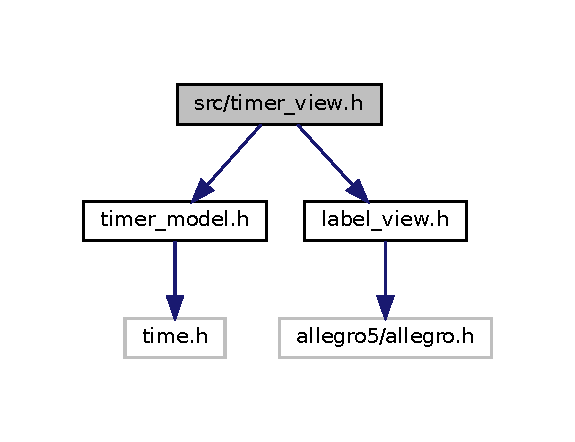
\includegraphics[width=276pt]{timer__view_8h__incl}
\end{center}
\end{figure}
Граф файлов, в которые включается этот файл\+:\nopagebreak
\begin{figure}[H]
\begin{center}
\leavevmode
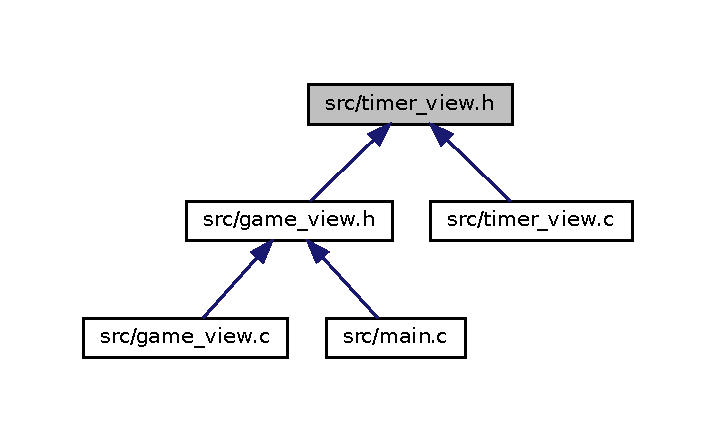
\includegraphics[width=344pt]{timer__view_8h__dep__incl}
\end{center}
\end{figure}
\subsection*{Структуры данных}
\begin{DoxyCompactItemize}
\item 
struct \hyperlink{structtimer__view}{timer\+\_\+view}
\begin{DoxyCompactList}\small\item\em Структура, которая описывает отображение таймеров. \end{DoxyCompactList}\end{DoxyCompactItemize}
\subsection*{Макросы}
\begin{DoxyCompactItemize}
\item 
\#define \hyperlink{timer__view_8h_aeb2e3603974f8cfe281b154e8e18a81b}{T\+I\+M\+E\+R\+\_\+\+B\+A\+C\+K\+G\+R\+O\+U\+N\+D\+\_\+\+C\+O\+L\+OR}~al\+\_\+map\+\_\+rgb(255, 255, 255)
\begin{DoxyCompactList}\small\item\em Цвет фона. \end{DoxyCompactList}\item 
\#define \hyperlink{timer__view_8h_a623c5765ad86a844b59daf12208dc0fe}{T\+I\+M\+E\+R\+\_\+\+B\+O\+R\+D\+E\+R\+\_\+\+C\+O\+L\+OR}~al\+\_\+map\+\_\+rgb(0, 0, 0)
\begin{DoxyCompactList}\small\item\em Цвет рамки. \end{DoxyCompactList}\item 
\#define \hyperlink{timer__view_8h_aa07a94b74fe29f66f358728e75c92120}{T\+I\+M\+E\+R\+\_\+\+T\+E\+X\+T\+\_\+\+C\+O\+L\+OR}~al\+\_\+map\+\_\+rgb(255, 99, 71)
\begin{DoxyCompactList}\small\item\em Цвет текста. \end{DoxyCompactList}\item 
\#define \hyperlink{timer__view_8h_a5d8bc42022f09d9f6183d24625eca939}{T\+I\+M\+E\+R\+\_\+\+W\+I\+D\+T\+H\+\_\+\+L\+T\+OP}~300
\begin{DoxyCompactList}\small\item\em Ширина таймера с рекордным времен. \end{DoxyCompactList}\item 
\#define \hyperlink{timer__view_8h_a1f0100f03a0debe0e6eb51f11ba0e54f}{T\+I\+M\+E\+R\+\_\+\+W\+I\+D\+T\+H\+\_\+\+L\+C\+U\+R\+R\+E\+NT}~200
\begin{DoxyCompactList}\small\item\em Ширина таймера с текущим времен. \end{DoxyCompactList}\item 
\#define \hyperlink{timer__view_8h_a6a0b0dd18b72fdb8ef9f7e438c057261}{T\+I\+M\+E\+R\+\_\+\+H\+E\+I\+G\+HT}~70
\begin{DoxyCompactList}\small\item\em Высота таймеров. \end{DoxyCompactList}\end{DoxyCompactItemize}
\subsection*{Определения типов}
\begin{DoxyCompactItemize}
\item 
typedef struct \hyperlink{structtimer__view}{timer\+\_\+view} \hyperlink{timer__view_8h_a834d6df554a53914ac021168c8e1e01d}{timer\+\_\+view}
\end{DoxyCompactItemize}
\subsection*{Функции}
\begin{DoxyCompactItemize}
\item 
\hyperlink{structtimer__view}{timer\+\_\+view} $\ast$ \hyperlink{timer__view_8h_ab60c31593d649a049480639234e40c3b}{timer\+\_\+view\+\_\+create} (\hyperlink{structtimer__model}{timer\+\_\+model} $\ast$t\+\_\+model, unsigned int width, unsigned int height, int shift\+\_\+x)
\item 
int \hyperlink{timer__view_8h_aa4c3cd871027bad94318899af57eca41}{timer\+\_\+view\+\_\+draw} (\hyperlink{structtimer__view}{timer\+\_\+view} $\ast$t\+\_\+view)
\item 
int \hyperlink{timer__view_8h_ae2233bb32211b932e7e3608ed0079407}{timer\+\_\+view\+\_\+destroy} (\hyperlink{structtimer__view}{timer\+\_\+view} $\ast$t\+\_\+view)
\end{DoxyCompactItemize}


\subsection{Подробное описание}
Файл, в котором опеределены функции для работы с отображением таймеров. 



\subsection{Макросы}
\mbox{\Hypertarget{timer__view_8h_aeb2e3603974f8cfe281b154e8e18a81b}\label{timer__view_8h_aeb2e3603974f8cfe281b154e8e18a81b}} 
\index{timer\+\_\+view.\+h@{timer\+\_\+view.\+h}!T\+I\+M\+E\+R\+\_\+\+B\+A\+C\+K\+G\+R\+O\+U\+N\+D\+\_\+\+C\+O\+L\+OR@{T\+I\+M\+E\+R\+\_\+\+B\+A\+C\+K\+G\+R\+O\+U\+N\+D\+\_\+\+C\+O\+L\+OR}}
\index{T\+I\+M\+E\+R\+\_\+\+B\+A\+C\+K\+G\+R\+O\+U\+N\+D\+\_\+\+C\+O\+L\+OR@{T\+I\+M\+E\+R\+\_\+\+B\+A\+C\+K\+G\+R\+O\+U\+N\+D\+\_\+\+C\+O\+L\+OR}!timer\+\_\+view.\+h@{timer\+\_\+view.\+h}}
\subsubsection{\texorpdfstring{T\+I\+M\+E\+R\+\_\+\+B\+A\+C\+K\+G\+R\+O\+U\+N\+D\+\_\+\+C\+O\+L\+OR}{TIMER\_BACKGROUND\_COLOR}}
{\footnotesize\ttfamily \#define T\+I\+M\+E\+R\+\_\+\+B\+A\+C\+K\+G\+R\+O\+U\+N\+D\+\_\+\+C\+O\+L\+OR~al\+\_\+map\+\_\+rgb(255, 255, 255)}



Цвет фона. 

\mbox{\Hypertarget{timer__view_8h_a623c5765ad86a844b59daf12208dc0fe}\label{timer__view_8h_a623c5765ad86a844b59daf12208dc0fe}} 
\index{timer\+\_\+view.\+h@{timer\+\_\+view.\+h}!T\+I\+M\+E\+R\+\_\+\+B\+O\+R\+D\+E\+R\+\_\+\+C\+O\+L\+OR@{T\+I\+M\+E\+R\+\_\+\+B\+O\+R\+D\+E\+R\+\_\+\+C\+O\+L\+OR}}
\index{T\+I\+M\+E\+R\+\_\+\+B\+O\+R\+D\+E\+R\+\_\+\+C\+O\+L\+OR@{T\+I\+M\+E\+R\+\_\+\+B\+O\+R\+D\+E\+R\+\_\+\+C\+O\+L\+OR}!timer\+\_\+view.\+h@{timer\+\_\+view.\+h}}
\subsubsection{\texorpdfstring{T\+I\+M\+E\+R\+\_\+\+B\+O\+R\+D\+E\+R\+\_\+\+C\+O\+L\+OR}{TIMER\_BORDER\_COLOR}}
{\footnotesize\ttfamily \#define T\+I\+M\+E\+R\+\_\+\+B\+O\+R\+D\+E\+R\+\_\+\+C\+O\+L\+OR~al\+\_\+map\+\_\+rgb(0, 0, 0)}



Цвет рамки. 

\mbox{\Hypertarget{timer__view_8h_a6a0b0dd18b72fdb8ef9f7e438c057261}\label{timer__view_8h_a6a0b0dd18b72fdb8ef9f7e438c057261}} 
\index{timer\+\_\+view.\+h@{timer\+\_\+view.\+h}!T\+I\+M\+E\+R\+\_\+\+H\+E\+I\+G\+HT@{T\+I\+M\+E\+R\+\_\+\+H\+E\+I\+G\+HT}}
\index{T\+I\+M\+E\+R\+\_\+\+H\+E\+I\+G\+HT@{T\+I\+M\+E\+R\+\_\+\+H\+E\+I\+G\+HT}!timer\+\_\+view.\+h@{timer\+\_\+view.\+h}}
\subsubsection{\texorpdfstring{T\+I\+M\+E\+R\+\_\+\+H\+E\+I\+G\+HT}{TIMER\_HEIGHT}}
{\footnotesize\ttfamily \#define T\+I\+M\+E\+R\+\_\+\+H\+E\+I\+G\+HT~70}



Высота таймеров. 

\mbox{\Hypertarget{timer__view_8h_aa07a94b74fe29f66f358728e75c92120}\label{timer__view_8h_aa07a94b74fe29f66f358728e75c92120}} 
\index{timer\+\_\+view.\+h@{timer\+\_\+view.\+h}!T\+I\+M\+E\+R\+\_\+\+T\+E\+X\+T\+\_\+\+C\+O\+L\+OR@{T\+I\+M\+E\+R\+\_\+\+T\+E\+X\+T\+\_\+\+C\+O\+L\+OR}}
\index{T\+I\+M\+E\+R\+\_\+\+T\+E\+X\+T\+\_\+\+C\+O\+L\+OR@{T\+I\+M\+E\+R\+\_\+\+T\+E\+X\+T\+\_\+\+C\+O\+L\+OR}!timer\+\_\+view.\+h@{timer\+\_\+view.\+h}}
\subsubsection{\texorpdfstring{T\+I\+M\+E\+R\+\_\+\+T\+E\+X\+T\+\_\+\+C\+O\+L\+OR}{TIMER\_TEXT\_COLOR}}
{\footnotesize\ttfamily \#define T\+I\+M\+E\+R\+\_\+\+T\+E\+X\+T\+\_\+\+C\+O\+L\+OR~al\+\_\+map\+\_\+rgb(255, 99, 71)}



Цвет текста. 

\mbox{\Hypertarget{timer__view_8h_a1f0100f03a0debe0e6eb51f11ba0e54f}\label{timer__view_8h_a1f0100f03a0debe0e6eb51f11ba0e54f}} 
\index{timer\+\_\+view.\+h@{timer\+\_\+view.\+h}!T\+I\+M\+E\+R\+\_\+\+W\+I\+D\+T\+H\+\_\+\+L\+C\+U\+R\+R\+E\+NT@{T\+I\+M\+E\+R\+\_\+\+W\+I\+D\+T\+H\+\_\+\+L\+C\+U\+R\+R\+E\+NT}}
\index{T\+I\+M\+E\+R\+\_\+\+W\+I\+D\+T\+H\+\_\+\+L\+C\+U\+R\+R\+E\+NT@{T\+I\+M\+E\+R\+\_\+\+W\+I\+D\+T\+H\+\_\+\+L\+C\+U\+R\+R\+E\+NT}!timer\+\_\+view.\+h@{timer\+\_\+view.\+h}}
\subsubsection{\texorpdfstring{T\+I\+M\+E\+R\+\_\+\+W\+I\+D\+T\+H\+\_\+\+L\+C\+U\+R\+R\+E\+NT}{TIMER\_WIDTH\_LCURRENT}}
{\footnotesize\ttfamily \#define T\+I\+M\+E\+R\+\_\+\+W\+I\+D\+T\+H\+\_\+\+L\+C\+U\+R\+R\+E\+NT~200}



Ширина таймера с текущим времен. 

\mbox{\Hypertarget{timer__view_8h_a5d8bc42022f09d9f6183d24625eca939}\label{timer__view_8h_a5d8bc42022f09d9f6183d24625eca939}} 
\index{timer\+\_\+view.\+h@{timer\+\_\+view.\+h}!T\+I\+M\+E\+R\+\_\+\+W\+I\+D\+T\+H\+\_\+\+L\+T\+OP@{T\+I\+M\+E\+R\+\_\+\+W\+I\+D\+T\+H\+\_\+\+L\+T\+OP}}
\index{T\+I\+M\+E\+R\+\_\+\+W\+I\+D\+T\+H\+\_\+\+L\+T\+OP@{T\+I\+M\+E\+R\+\_\+\+W\+I\+D\+T\+H\+\_\+\+L\+T\+OP}!timer\+\_\+view.\+h@{timer\+\_\+view.\+h}}
\subsubsection{\texorpdfstring{T\+I\+M\+E\+R\+\_\+\+W\+I\+D\+T\+H\+\_\+\+L\+T\+OP}{TIMER\_WIDTH\_LTOP}}
{\footnotesize\ttfamily \#define T\+I\+M\+E\+R\+\_\+\+W\+I\+D\+T\+H\+\_\+\+L\+T\+OP~300}



Ширина таймера с рекордным времен. 



\subsection{Типы}
\mbox{\Hypertarget{timer__view_8h_a834d6df554a53914ac021168c8e1e01d}\label{timer__view_8h_a834d6df554a53914ac021168c8e1e01d}} 
\index{timer\+\_\+view.\+h@{timer\+\_\+view.\+h}!timer\+\_\+view@{timer\+\_\+view}}
\index{timer\+\_\+view@{timer\+\_\+view}!timer\+\_\+view.\+h@{timer\+\_\+view.\+h}}
\subsubsection{\texorpdfstring{timer\+\_\+view}{timer\_view}}
{\footnotesize\ttfamily typedef struct \hyperlink{structtimer__view}{timer\+\_\+view} \hyperlink{structtimer__view}{timer\+\_\+view}}



\subsection{Функции}
\mbox{\Hypertarget{timer__view_8h_ab60c31593d649a049480639234e40c3b}\label{timer__view_8h_ab60c31593d649a049480639234e40c3b}} 
\index{timer\+\_\+view.\+h@{timer\+\_\+view.\+h}!timer\+\_\+view\+\_\+create@{timer\+\_\+view\+\_\+create}}
\index{timer\+\_\+view\+\_\+create@{timer\+\_\+view\+\_\+create}!timer\+\_\+view.\+h@{timer\+\_\+view.\+h}}
\subsubsection{\texorpdfstring{timer\+\_\+view\+\_\+create()}{timer\_view\_create()}}
{\footnotesize\ttfamily \hyperlink{structtimer__view}{timer\+\_\+view}$\ast$ timer\+\_\+view\+\_\+create (\begin{DoxyParamCaption}\item[{\hyperlink{structtimer__model}{timer\+\_\+model} $\ast$}]{t\+\_\+model,  }\item[{unsigned int}]{width,  }\item[{unsigned int}]{height,  }\item[{int}]{shift\+\_\+x }\end{DoxyParamCaption})}

Создание отображения таймеров. 
\begin{DoxyParams}[1]{Аргументы}
\mbox{\tt in}  & {\em t\+\_\+model} & -\/ адрес модели таймеров. \\
\hline
\mbox{\tt in}  & {\em width} & -\/ ширина области рисования. \\
\hline
\mbox{\tt in}  & {\em height} & -\/ высота области рисования. \\
\hline
\mbox{\tt in}  & {\em shift\+\_\+x} & -\/ смещение позиций рисования таймеров по оси OX. \\
\hline
\end{DoxyParams}
\begin{DoxyReturn}{Возвращает}
Адрес, созданного отображения таймеров. ~\newline
 N\+U\+LL, если во время создания отображения таймеров произошла ошибка. 
\end{DoxyReturn}
\mbox{\Hypertarget{timer__view_8h_ae2233bb32211b932e7e3608ed0079407}\label{timer__view_8h_ae2233bb32211b932e7e3608ed0079407}} 
\index{timer\+\_\+view.\+h@{timer\+\_\+view.\+h}!timer\+\_\+view\+\_\+destroy@{timer\+\_\+view\+\_\+destroy}}
\index{timer\+\_\+view\+\_\+destroy@{timer\+\_\+view\+\_\+destroy}!timer\+\_\+view.\+h@{timer\+\_\+view.\+h}}
\subsubsection{\texorpdfstring{timer\+\_\+view\+\_\+destroy()}{timer\_view\_destroy()}}
{\footnotesize\ttfamily int timer\+\_\+view\+\_\+destroy (\begin{DoxyParamCaption}\item[{\hyperlink{structtimer__view}{timer\+\_\+view} $\ast$}]{t\+\_\+view }\end{DoxyParamCaption})}

Удаление отображения таймеров. 
\begin{DoxyParams}[1]{Аргументы}
\mbox{\tt in}  & {\em t\+\_\+view} & -\/ адрес отображения таймеров, которое нужно удалить. \\
\hline
\end{DoxyParams}
\begin{DoxyReturn}{Возвращает}
Ноль, если удаление прошло успешно. ~\newline
 Ненулевое число, если во время удаления произошла ошибка. 
\end{DoxyReturn}
\mbox{\Hypertarget{timer__view_8h_aa4c3cd871027bad94318899af57eca41}\label{timer__view_8h_aa4c3cd871027bad94318899af57eca41}} 
\index{timer\+\_\+view.\+h@{timer\+\_\+view.\+h}!timer\+\_\+view\+\_\+draw@{timer\+\_\+view\+\_\+draw}}
\index{timer\+\_\+view\+\_\+draw@{timer\+\_\+view\+\_\+draw}!timer\+\_\+view.\+h@{timer\+\_\+view.\+h}}
\subsubsection{\texorpdfstring{timer\+\_\+view\+\_\+draw()}{timer\_view\_draw()}}
{\footnotesize\ttfamily int timer\+\_\+view\+\_\+draw (\begin{DoxyParamCaption}\item[{\hyperlink{structtimer__view}{timer\+\_\+view} $\ast$}]{t\+\_\+view }\end{DoxyParamCaption})}

Рисование отображения таймеров. 
\begin{DoxyParams}[1]{Аргументы}
\mbox{\tt in}  & {\em t\+\_\+view} & -\/ адрес отображения таймеров, которое нужно нарисовать. \\
\hline
\end{DoxyParams}
\begin{DoxyReturn}{Возвращает}
Ноль, если отображение было успешно отрисовано. ~\newline
 Ненулевое число, если во время рисования произошла ошибка. 
\end{DoxyReturn}

%--- End generated contents ---

% Index
\backmatter
\newpage
\phantomsection
\clearemptydoublepage
\addcontentsline{toc}{chapter}{Алфавитный указатель}
\printindex

\end{document}
